%=====================================================================
% Análisis de funcionalidades CRUD
%=====================================================================
\section*{Análisis de funcionalidades CRUD}
\addcontentsline{toc}{section}{Análisis de funcionalidades CRUD}

Esta sección identifica las funcionalidades del sistema que crean, consultan, actualizan o eliminan información, y describe cada una en un prototipo de análisis: quién la ejecuta, qué datos recibe, qué datos lee y escribe, qué reglas debe respetar y qué resultado produce. Es el insumo directo del modelo de datos: todo atributo que aparece aquí debe existir en alguna tabla, y toda tabla debe estar justificada por al menos una funcionalidad.

Cada funcionalidad remite al caso de uso donde se describe su comportamiento completo. Las entidades se escriben en cursiva y los atributos en tipografía de código; los nombres de ambos no llevan acentos ni eñes porque son identificadores de la base de datos. Las reglas de negocio se citan con el número que tienen en su caso de uso, por ejemplo \textit{\mbox{CU-03} \mbox{RN-07}}, y las decisiones de diseño con su identificador, por ejemplo \textit{\mbox{D-01}}.

Las 53 funcionalidades cubren los 49 casos de uso del sistema salvo uno: enviar un emote (\mbox{CU-29}) no lee ni escribe en la base de datos (\mbox{D-10}), así que no tiene prototipo de análisis.

Cada prototipo de análisis va acompañado de las pantallas del prototipo de interfaz que lo ilustran. De las 125 pantallas diseñadas se usan 57; la sección \textit{Trazabilidad de prototipos}, al final de este apartado, indica a qué funcionalidad corresponde cada una y por qué se descartaron las demás.

\subsection*{Resumen de operaciones por objeto de información}
\addcontentsline{toc}{subsection}{Resumen de operaciones por objeto de información}

La tabla indica qué funcionalidad realiza cada operación sobre cada objeto de información. Una celda vacía significa que la operación no existe desde la aplicación, y la sección siguiente explica por qué.

\begin{center}\small
\begin{longtable}{|L{0.22\textwidth}|L{0.18\textwidth}|L{0.13\textwidth}|L{0.22\textwidth}|L{0.13\textwidth}|}
\hline
\textbf{Objeto de información} & \textbf{Crear} & \textbf{Consultar} & \textbf{Actualizar} & \textbf{Eliminar} \\ \hline
\endfirsthead
\hline
\textbf{Objeto de información} & \textbf{Crear} & \textbf{Consultar} & \textbf{Actualizar} & \textbf{Eliminar} \\ \hline
\endhead
Cuenta de usuario & \mbox{F-01}, \mbox{F-02} & \mbox{F-06} & \mbox{F-03}, \mbox{F-04}, \mbox{F-05}, \mbox{F-07}, \mbox{F-08}, \mbox{F-09}, \mbox{F-10}, \mbox{F-11}, \mbox{F-13} & \mbox{F-12} (lógica) \\ \hline
Tokens y códigos de acceso & \mbox{F-01}, \mbox{F-03}, \mbox{F-09}, \mbox{F-11}, \mbox{F-14} & \mbox{F-04} & \mbox{F-04}, \mbox{F-09}, \mbox{F-11} &  \\ \hline
Sesión & \mbox{F-02}, \mbox{F-14} & \mbox{F-15} &  & \mbox{F-16} (lógica) \\ \hline
Cola de emparejamiento & \mbox{F-17} &  &  & \mbox{F-17}, \mbox{F-18} \\ \hline
Salas e invitaciones & \mbox{F-19}, \mbox{F-20}, \mbox{F-21} & \mbox{F-20} & \mbox{F-19}, \mbox{F-20}, \mbox{F-21} & \mbox{F-19}, \mbox{F-20}, \mbox{F-43} \\ \hline
Partida y participaciones & \mbox{F-17}, \mbox{F-19}, \mbox{F-27} & \mbox{F-26}, \mbox{F-29} & \mbox{F-24}, \mbox{F-25}, \mbox{F-26}, \mbox{F-28} &  \\ \hline
Jugadas & \mbox{F-22}, \mbox{F-27} & \mbox{F-30}, \mbox{F-31} & \mbox{F-27} &  \\ \hline
Ofertas de tablas & \mbox{F-23} &  & \mbox{F-22}, \mbox{F-23} &  \\ \hline
Enlaces de espectador & \mbox{F-31} & \mbox{F-31} & \mbox{F-28} &  \\ \hline
Estadísticas y divisiones & \mbox{F-01}, \mbox{F-02}, \mbox{F-28} & \mbox{F-06}, \mbox{F-32} & \mbox{F-25}, \mbox{F-28} &  \\ \hline
Avatar y enlaces del perfil & \mbox{F-07} & \mbox{F-06} & \mbox{F-07} & \mbox{F-07} \\ \hline
Objetos y equipamiento & \mbox{F-01}, \mbox{F-34}, \mbox{F-35} & \mbox{F-37} & \mbox{F-05}, \mbox{F-07}, \mbox{F-36} &  \\ \hline
Monedas y cajas & \mbox{F-28}, \mbox{F-34}, \mbox{F-35} & \mbox{F-37}, \mbox{F-38} & \mbox{F-35} &  \\ \hline
Progreso del tutorial & \mbox{F-33} & \mbox{F-33} & \mbox{F-33} &  \\ \hline
Solicitudes y amistades & \mbox{F-39}, \mbox{F-40} & \mbox{F-41} &  & \mbox{F-40}, \mbox{F-42}, \mbox{F-43} \\ \hline
Silencios y bloqueos & \mbox{F-43} & \mbox{F-44}, \mbox{F-45} &  & \mbox{F-43} \\ \hline
Mensajes & \mbox{F-19}, \mbox{F-31}, \mbox{F-44} & \mbox{F-45} &  &  \\ \hline
Reportes & \mbox{F-46} & \mbox{F-47} & \mbox{F-47}, \mbox{F-48} &  \\ \hline
Sanciones y apelaciones & \mbox{F-48}, \mbox{F-49} & \mbox{F-47} & \mbox{F-48}, \mbox{F-50} &  \\ \hline
Roles de moderación &  &  & \mbox{F-51}, \mbox{F-52} &  \\ \hline
Bitácoras & varias & \mbox{F-53} &  &  \\ \hline
\end{longtable}
\end{center}

\subsection*{Criterio de eliminación}
\addcontentsline{toc}{subsection}{Criterio de eliminación}

El sistema distingue dos formas de eliminar, y la elección no es indiferente para el modelo de datos.

\begin{reglas}
  \item \textbf{Eliminación lógica.} La fila se conserva y cambia de estado. Se aplica a lo que otros registros necesitan seguir referenciando o a lo que tiene valor como evidencia: la cuenta pasa a \texttt{ELIMINADA} y después se anonimiza (\mbox{F-12}), la sesión recibe \texttt{fecha\_\allowbreak{}fin} (\mbox{F-16}), la sala pasa a \texttt{CERRADA} (\mbox{F-19}), la sanción retirada pasa a \texttt{activa} = 0 (\mbox{F-48}, \mbox{F-50}) y el avatar sustituido pasa a \texttt{vigente} = 0 (\mbox{F-07}). Borrar una cuenta físicamente arrastraría por clave foránea las partidas, las jugadas y los mensajes de los demás jugadores que participaron en ellas.
  \item \textbf{Eliminación física.} La fila desaparece. Se aplica a lo que describe un estado presente y no un hecho pasado: la entrada en la cola de emparejamiento (\mbox{F-17}, \mbox{F-18}), la plaza en una sala (\mbox{F-19}, \mbox{F-20}), una solicitud ya respondida (\mbox{F-40}), una amistad terminada (\mbox{F-42}), un silencio o un bloqueo retirados (\mbox{F-43}) y un enlace quitado del perfil (\mbox{F-07}). Conservar esas filas no aporta información y obligaría a filtrarlas en cada consulta.
  \item \textbf{Sin eliminación.} Jugadas, ofertas de tablas, invitaciones, movimientos de monedas, reportes, apelaciones y bitácoras nunca se eliminan ni se modifican desde la aplicación más allá de su estado. Una jugada deshecha contra la IA se marca, no se borra (\mbox{F-27}), y una corrección de monedas es un movimiento nuevo (\mbox{F-38}).
\end{reglas}

\subsection*{Cuenta de usuario}
\addcontentsline{toc}{subsection}{Cuenta de usuario}

La cuenta es el objeto de información central: casi todas las demás estructuras dependen de ella. Se crea por dos vías —registro e invitado—, se modifica por nueve funcionalidades distintas y nunca se elimina físicamente: la baja es lógica y, pasado el plazo de recuperación, la cuenta se anonimiza.

%--- F-01 Registrar cuenta
\begin{prototipocrud}{F-01}{Registrar cuenta}
  \crudFila{Operación}{Creación (C)}
  \crudFila{Caso de uso}{\mbox{CU-02}}
  \crudFila{Actor}{Jugador sin cuenta}
  \crudFila{Prototipos}{Sin prototipo. La pantalla 6c solo ofrece la opción ``crear cuenta''; el formulario de registro no está prototipado.}
  \crudFila{Datos de entrada}{\begin{crudlista}
    \item \texttt{nickname}: texto de 3 a 30 caracteres, sin espacios.
    \item \texttt{correo}: texto de hasta 254 caracteres con formato de correo.
    \item Contraseña y su confirmación: texto de al menos 8 caracteres. No se almacena.
    \item \texttt{fecha\_\allowbreak{}nacimiento}: fecha.
    \item \texttt{idioma\_\allowbreak{}preferido}: código de cultura, por ejemplo \texttt{es-MX}.
    \item Versión de los términos de uso aceptada.
    \item Huella del dispositivo y \texttt{version\_\allowbreak{}cliente}, que envía el cliente sin intervención del jugador.
  \end{crudlista}}
  \crudFila{Datos que se consultan}{\begin{crudlista}
    \item \textit{Usuario}: \texttt{nickname} y \texttt{correo} de las cuentas existentes, para comprobar unicidad.
    \item \textit{PalabraProhibida}: \texttt{termino}, \texttt{idioma}, \texttt{ambito} y \texttt{activo}, para filtrar el \texttt{nickname}.
    \item \textit{ObjetoCosmetico}: los marcados con \texttt{es\_\allowbreak{}inicial} y el marcado con \texttt{es\_\allowbreak{}predeterminado} en cada \textit{Ranura}.
    \item \textit{Modo}: los modos activos.
  \end{crudlista}}
  \crudFila{Datos que se crean}{\begin{crudlista}
    \item \textit{Usuario}: \texttt{tipo\_\allowbreak{}cuenta} = \texttt{REGISTRADA}, \texttt{estado\_\allowbreak{}cuenta} = \texttt{PENDIENTE}, \texttt{rol} = \texttt{JUGADOR}, \texttt{nickname}, \texttt{correo}, \texttt{contrasena\_\allowbreak{}hash}, \texttt{contrasena\_\allowbreak{}sal}, \texttt{fecha\_\allowbreak{}nacimiento}, \texttt{idioma\_\allowbreak{}preferido}, \texttt{codigo\_\allowbreak{}amigo}, \texttt{fecha\_\allowbreak{}registro}; \texttt{intentos\_\allowbreak{}fallidos}, \texttt{experiencia} y \texttt{saldo\_\allowbreak{}monedas} en cero; \texttt{nivel} en 1; \texttt{fecha\_\allowbreak{}configuracion\_\allowbreak{}inicial} y \texttt{bloqueada\_\allowbreak{}hasta} en nulo; \texttt{doble\_\allowbreak{}factor\_\allowbreak{}habilitado} en falso.
    \item \textit{EstadisticaModo}: una por cada \textit{Modo}, con los contadores en cero y el elo inicial.
    \item \textit{UsuarioObjeto}: uno por cada objeto inicial, con \texttt{origen} = \texttt{INICIAL}.
    \item \textit{Equipamiento}: una fila por cada una de las seis \textit{Ranura}, apuntando al objeto predeterminado.
    \item \textit{AceptacionTerminos}: \texttt{version\_\allowbreak{}terminos}, \texttt{fecha\_\allowbreak{}aceptacion}, \texttt{direccion\_\allowbreak{}ip}.
    \item \textit{TokenVerificacionCorreo}: \texttt{token\_\allowbreak{}hash}, \texttt{proposito} = \texttt{ALTA}, \texttt{fecha\_\allowbreak{}expiracion}, \texttt{usado} = 0.
    \item \textit{BitacoraAcceso}: \texttt{REGISTRO\_\allowbreak{}EXITOSO}, \texttt{REGISTRO\_\allowbreak{}RECHAZADO} o \texttt{REGISTRO\_\allowbreak{}SIN\_\allowbreak{}CORREO}.
  \end{crudlista}}
  \crudFila{Datos que se modifican}{\begin{crudlista}
    \item \textit{Usuario}: \texttt{fecha\_\allowbreak{}ultimo\_\allowbreak{}envio\_\allowbreak{}verificacion}, una vez enviado el correo.
  \end{crudlista}}
  \crudFila{Datos que se eliminan}{Ninguno.}
  \crudFila{Reglas de negocio}{\begin{crudlista}
    \item El \texttt{nickname} es único y se compara sin distinguir mayúsculas ni acentos (\mbox{CU-02} \mbox{RN-01}).
    \item El \texttt{correo} es único y se normaliza a minúsculas (\mbox{CU-02} \mbox{RN-02}).
    \item La contraseña combina al menos tres de cuatro grupos de caracteres y nunca se guarda en claro (\mbox{CU-02} \mbox{RN-03}).
    \item La edad mínima es de ocho años, calculada desde \texttt{fecha\_\allowbreak{}nacimiento} (\mbox{CU-02} \mbox{RN-05}).
    \item Toda cuenta nace en \texttt{PENDIENTE} (\mbox{CU-02} \mbox{RN-04}).
    \item El alta completa ocurre en una sola transacción (\mbox{CU-02} \mbox{RN-06}).
    \item No se piden apellidos ni región (\mbox{D-06}).
  \end{crudlista}}
  \crudFila{Resultado esperado}{Existe una cuenta en \texttt{PENDIENTE} con sus estadísticas en cero, sus objetos iniciales, uno equipado en cada ranura y los términos aceptados. Se envió el correo de verificación. El jugador no puede iniciar sesión hasta verificarlo.}
\end{prototipocrud}

%--- F-02 Crear cuenta de invitado
\begin{prototipocrud}{F-02}{Crear cuenta de invitado}
  \crudFila{Operación}{Creación (C)}
  \crudFila{Caso de uso}{\mbox{CU-06}}
  \crudFila{Actor}{Invitado}
  \crudFila{Prototipos}{6c, la opción ``jugar como invitado'' (\mbox{F-14}).}
  \crudFila{Datos de entrada}{\begin{crudlista}
    \item Ninguna captura del jugador: basta con elegir la opción.
    \item Huella del dispositivo y \texttt{version\_\allowbreak{}cliente}.
  \end{crudlista}}
  \crudFila{Datos que se consultan}{\begin{crudlista}
    \item \textit{Usuario}: \texttt{nickname}, para comprobar que el provisional esté libre.
    \item \textit{BitacoraAcceso}: altas de invitado desde la misma \texttt{direccion\_\allowbreak{}ip} en la última hora.
    \item \textit{Modo}, \textit{Ranura} y \textit{ObjetoCosmetico} iniciales y predeterminados.
  \end{crudlista}}
  \crudFila{Datos que se crean}{\begin{crudlista}
    \item \textit{Usuario}: \texttt{tipo\_\allowbreak{}cuenta} = \texttt{INVITADO}, \texttt{estado\_\allowbreak{}cuenta} = \texttt{ACTIVA}, \texttt{rol} = \texttt{JUGADOR}, \texttt{nickname} provisional, \texttt{fecha\_\allowbreak{}registro}; \texttt{correo}, \texttt{contrasena\_\allowbreak{}hash} y \texttt{contrasena\_\allowbreak{}sal} en nulo.
    \item \textit{EstadisticaModo}, \textit{UsuarioObjeto} y \textit{Equipamiento}, igual que al registrar una cuenta.
    \item \textit{Sesion}: \texttt{token\_\allowbreak{}hash}, \texttt{fecha\_\allowbreak{}inicio}, \texttt{fecha\_\allowbreak{}expiracion}, \texttt{direccion\_\allowbreak{}ip}, \texttt{huella\_\allowbreak{}dispositivo}, \texttt{version\_\allowbreak{}cliente}.
    \item \textit{BitacoraAcceso}: \texttt{resultado} = \texttt{ALTA\_\allowbreak{}INVITADO}.
  \end{crudlista}}
  \crudFila{Datos que se modifican}{Ninguno.}
  \crudFila{Datos que se eliminan}{Ninguno.}
  \crudFila{Reglas de negocio}{\begin{crudlista}
    \item El invitado no tiene correo ni contraseña; su cuenta vive atada al token guardado en el dispositivo (\mbox{CU-06} \mbox{RN-03}, \mbox{RN-04}).
    \item Acumula elo, monedas, objetos y partidas igual que una cuenta registrada (\mbox{CU-06} \mbox{RN-05}).
    \item Las altas de invitado por dirección de red están acotadas por hora (\mbox{CU-06} \mbox{RN-07}).
    \item El \texttt{nickname} provisional usa un formato reservado (\mbox{CU-06} \mbox{RN-02}).
  \end{crudlista}}
  \crudFila{Resultado esperado}{El invitado juega de inmediato, con sesión abierta y un aviso permanente de que perderá el progreso si no vincula la cuenta.}
\end{prototipocrud}

%--- F-03 Vincular cuenta de invitado
\begin{prototipocrud}{F-03}{Vincular cuenta de invitado}
  \crudFila{Operación}{Actualización (U)}
  \crudFila{Caso de uso}{\mbox{CU-07}}
  \crudFila{Actor}{Invitado}
  \crudFila{Prototipos}{9e, Invitado · vincular cuenta.}
  \crudFila{Datos de entrada}{\begin{crudlista}
    \item \texttt{nickname} definitivo, \texttt{correo}, contraseña y confirmación, \texttt{fecha\_\allowbreak{}nacimiento}: mismos formatos que al registrar.
    \item Versión de los términos aceptada.
    \item Token de la sesión de invitado.
  \end{crudlista}}
  \crudFila{Datos que se consultan}{\begin{crudlista}
    \item \textit{Sesion}: la del token, que debe pertenecer a un \textit{Usuario} con \texttt{tipo\_\allowbreak{}cuenta} = \texttt{INVITADO}.
    \item \textit{Usuario}: \texttt{nickname} y \texttt{correo} de las demás cuentas.
    \item \textit{PalabraProhibida}.
  \end{crudlista}}
  \crudFila{Datos que se crean}{\begin{crudlista}
    \item \textit{AceptacionTerminos}.
    \item \textit{TokenVerificacionCorreo} con \texttt{proposito} = \texttt{ALTA}.
    \item \textit{BitacoraAcceso}: \texttt{resultado} = \texttt{VINCULACION\_\allowbreak{}EXITOSA}.
  \end{crudlista}}
  \crudFila{Datos que se modifican}{\begin{crudlista}
    \item \textit{Usuario}: \texttt{tipo\_\allowbreak{}cuenta} pasa a \texttt{REGISTRADA} y \texttt{estado\_\allowbreak{}cuenta} a \texttt{PENDIENTE}; se escriben \texttt{nickname}, \texttt{correo}, \texttt{contrasena\_\allowbreak{}hash}, \texttt{contrasena\_\allowbreak{}sal}, \texttt{fecha\_\allowbreak{}nacimiento} y \texttt{fecha\_\allowbreak{}ultimo\_\allowbreak{}envio\_\allowbreak{}verificacion}.
    \item \textit{Sesion} de invitado: \texttt{fecha\_\allowbreak{}fin} y \texttt{motivo\_\allowbreak{}cierre} = \texttt{CAMBIO\_\allowbreak{}CREDENCIALES}.
  \end{crudlista}}
  \crudFila{Datos que se eliminan}{Ninguno.}
  \crudFila{Reglas de negocio}{\begin{crudlista}
    \item Se actualiza el mismo \textit{Usuario} conservando su \texttt{id\_\allowbreak{}usuario}; no se copia ni se mueve ninguna fila (\mbox{CU-07} \mbox{RN-01}).
    \item No puede vincularse a un correo ya registrado (\mbox{CU-07} \mbox{RN-05}).
    \item La cuenta vinculada nace en \texttt{PENDIENTE} (\mbox{CU-07} \mbox{RN-04}).
    \item Vincular cierra la sesión de invitado (\mbox{CU-07} \mbox{RN-08}).
  \end{crudlista}}
  \crudFila{Resultado esperado}{La cuenta conserva íntegros su elo, sus monedas, sus objetos y su historial, queda registrada y pendiente de verificación.}
\end{prototipocrud}
\par\nopagebreak\smallskip
\begin{center}
\begin{minipage}[t]{0.50\textwidth}\centering
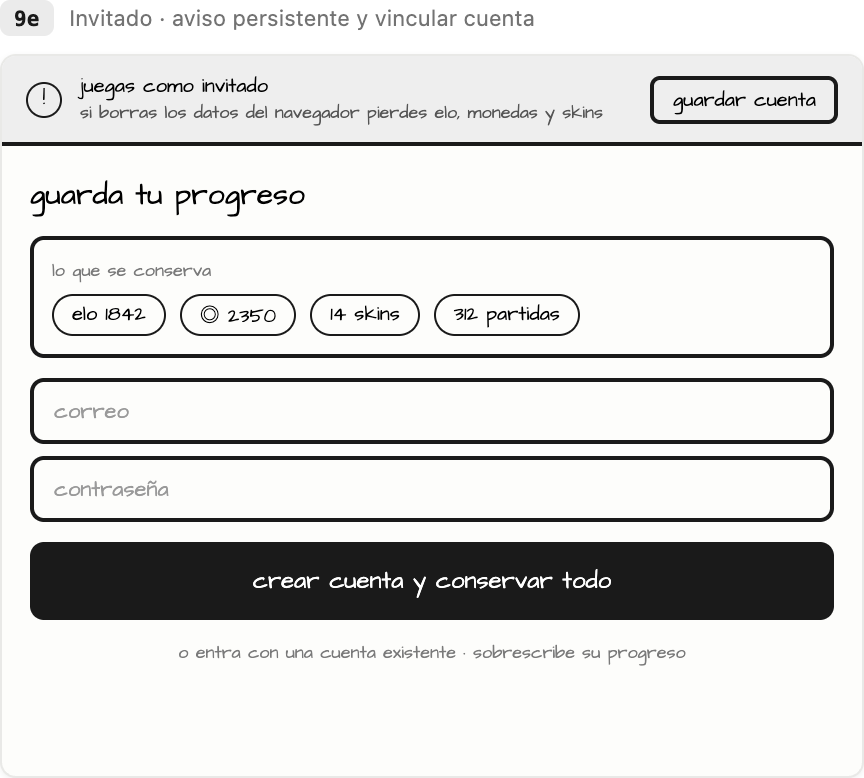
\includegraphics[width=\linewidth]{Prototipos/9e}\par\smallskip
{\footnotesize\textit{Prototipo 9e: Invitado · vincular cuenta}}
\end{minipage}
\par\medskip
\end{center}

%--- F-04 Verificar correo
\begin{prototipocrud}{F-04}{Verificar correo}
  \crudFila{Operación}{Actualización (U)}
  \crudFila{Caso de uso}{\mbox{CU-04}}
  \crudFila{Actor}{Jugador}
  \crudFila{Prototipos}{Sin prototipo: ocurre fuera del juego, en la página que abre el enlace del correo.}
  \crudFila{Datos de entrada}{\begin{crudlista}
    \item Token incluido en el enlace del correo.
  \end{crudlista}}
  \crudFila{Datos que se consultan}{\begin{crudlista}
    \item \textit{TokenVerificacionCorreo}: \texttt{token\_\allowbreak{}hash}, \texttt{proposito}, \texttt{correo\_\allowbreak{}destino}, \texttt{usado}, \texttt{fecha\_\allowbreak{}expiracion}.
    \item \textit{Usuario}: \texttt{estado\_\allowbreak{}cuenta}, \texttt{idioma\_\allowbreak{}preferido}.
    \item \textit{Sancion}: activas con \texttt{ambito} = \texttt{CUENTA}.
  \end{crudlista}}
  \crudFila{Datos que se crean}{\begin{crudlista}
    \item \textit{BitacoraAcceso}: \texttt{resultado} = \texttt{CUENTA\_\allowbreak{}VERIFICADA}.
  \end{crudlista}}
  \crudFila{Datos que se modifican}{\begin{crudlista}
    \item \textit{Usuario}: \texttt{estado\_\allowbreak{}cuenta} pasa de \texttt{PENDIENTE} a \texttt{ACTIVA}; se escribe \texttt{fecha\_\allowbreak{}verificacion}.
    \item \textit{TokenVerificacionCorreo}: \texttt{usado} = 1, y los demás pendientes del usuario quedan invalidados.
  \end{crudlista}}
  \crudFila{Datos que se eliminan}{Ninguno.}
  \crudFila{Reglas de negocio}{\begin{crudlista}
    \item El token es de un solo uso y vale veinticuatro horas (\mbox{CU-04} \mbox{RN-01}, \mbox{RN-02}).
    \item Es el único flujo que lleva una cuenta a \texttt{ACTIVA} (\mbox{CU-04} \mbox{RN-07}).
    \item Verificar no levanta sanciones ni abre sesión (\mbox{CU-04} \mbox{RN-05}).
    \item Un enlace inválido, caducado o de una cuenta eliminada produce la misma respuesta (\mbox{CU-04} \mbox{RN-04}).
  \end{crudlista}}
  \crudFila{Resultado esperado}{La cuenta queda \texttt{ACTIVA} y el jugador puede iniciar sesión.}
\end{prototipocrud}

%--- F-05 Configurar la cuenta la primera vez
\begin{prototipocrud}{F-05}{Configurar la cuenta la primera vez}
  \crudFila{Operación}{Actualización (U)}
  \crudFila{Caso de uso}{\mbox{CU-08}}
  \crudFila{Actor}{Jugador o invitado}
  \crudFila{Prototipos}{6d, Primera vez · nombre, peón e icono.}
  \crudFila{Datos de entrada}{\begin{crudlista}
    \item \texttt{id\_\allowbreak{}objeto} del peón elegido, opcional.
    \item \texttt{id\_\allowbreak{}icono}: entero de 1 a 32, opcional.
    \item Token de sesión.
  \end{crudlista}}
  \crudFila{Datos que se consultan}{\begin{crudlista}
    \item \textit{Usuario}: \texttt{fecha\_\allowbreak{}configuracion\_\allowbreak{}inicial}, que debe ser nula.
    \item \textit{UsuarioObjeto} y \textit{ObjetoCosmetico}: los peones iniciales que posee el usuario.
  \end{crudlista}}
  \crudFila{Datos que se crean}{Ninguno.}
  \crudFila{Datos que se modifican}{\begin{crudlista}
    \item \textit{Equipamiento}: la fila de la ranura de peón apunta al peón elegido.
    \item \textit{Usuario}: \texttt{id\_\allowbreak{}icono} y \texttt{fecha\_\allowbreak{}configuracion\_\allowbreak{}inicial}.
  \end{crudlista}}
  \crudFila{Datos que se eliminan}{Ninguno.}
  \crudFila{Reglas de negocio}{\begin{crudlista}
    \item La configuración inicial se ofrece una sola vez por cuenta (\mbox{CU-08} \mbox{RN-01}).
    \item El peón debe ser un objeto inicial ya poseído; esta funcionalidad no otorga objetos (\mbox{CU-08} \mbox{RN-02}).
    \item Omitirla es válido y conserva los predeterminados (\mbox{CU-08} \mbox{RN-04}).
    \item El \texttt{nickname} no se elige aquí (\mbox{D-13}).
  \end{crudlista}}
  \crudFila{Resultado esperado}{El jugador entra al menú con el peón y el icono elegidos, y la pantalla de primera vez no vuelve a aparecer en ningún dispositivo.}
\end{prototipocrud}
\par\nopagebreak\smallskip
\begin{center}
\begin{minipage}[t]{0.50\textwidth}\centering
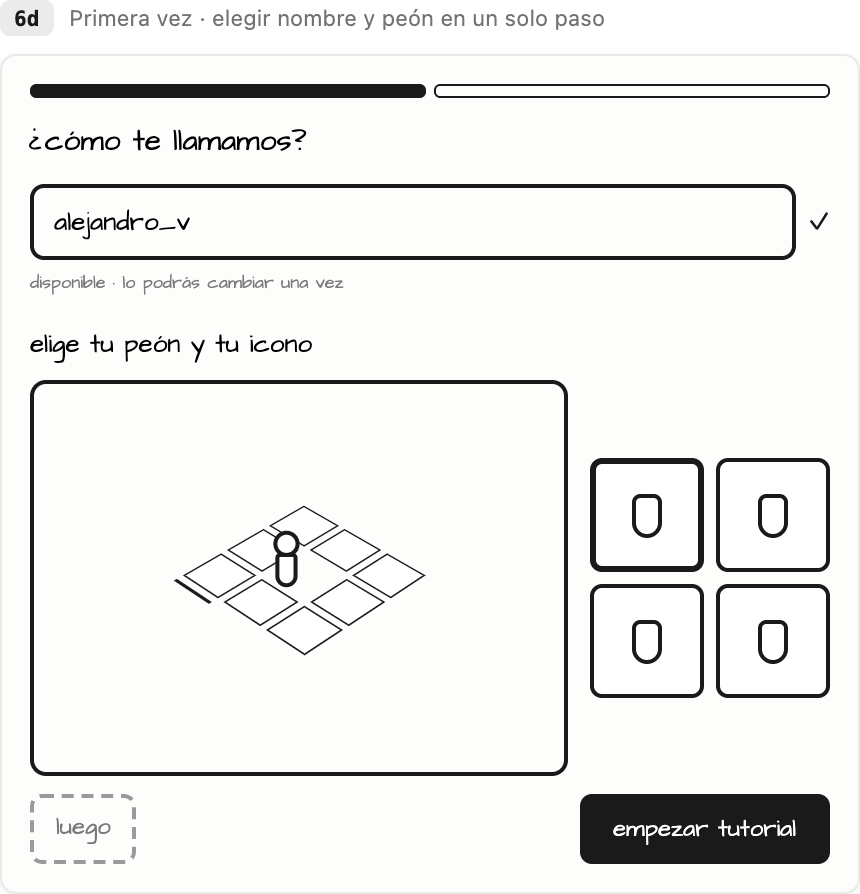
\includegraphics[width=\linewidth]{Prototipos/6d}\par\smallskip
{\footnotesize\textit{Prototipo 6d: Primera vez · nombre, peón e icono}}
\end{minipage}
\par\medskip
\end{center}

%--- F-06 Consultar perfil de un jugador
\begin{prototipocrud}{F-06}{Consultar perfil de un jugador}
  \crudFila{Operación}{Consulta (R)}
  \crudFila{Caso de uso}{\mbox{CU-15}, \mbox{CU-16}}
  \crudFila{Actor}{Jugador o invitado}
  \crudFila{Prototipos}{5a, Perfil propio · estadísticas y títulos; 5b, Perfil de otro jugador · historial común; 16c, Evolución del elo.}
  \crudFila{Datos de entrada}{\begin{crudlista}
    \item \texttt{id\_\allowbreak{}usuario} del jugador consultado, o ninguno para el perfil propio.
    \item Modo de la gráfica de elo, opcional.
    \item Token de sesión.
  \end{crudlista}}
  \crudFila{Datos que se consultan}{\begin{crudlista}
    \item \textit{Usuario}: \texttt{nickname}, \texttt{nivel}, \texttt{experiencia}, \texttt{id\_\allowbreak{}icono}, \texttt{fecha\_\allowbreak{}registro}, \texttt{tipo\_\allowbreak{}cuenta}, \texttt{estado\_\allowbreak{}cuenta}.
    \item \textit{Avatar} vigente, \textit{EnlaceRed} y, de \textit{Equipamiento}, el título y el marco.
    \item \textit{EstadisticaModo}, por modo: \texttt{partidas\_\allowbreak{}jugadas}, \texttt{partidas\_\allowbreak{}ganadas}, \texttt{partidas\_\allowbreak{}perdidas}, \texttt{puntos\_\allowbreak{}elo}, \texttt{elo\_\allowbreak{}maximo}, \texttt{racha\_\allowbreak{}actual}, \texttt{mejor\_\allowbreak{}racha}, \texttt{division}.
    \item \textit{Division}: \texttt{elo\_\allowbreak{}minimo} y \texttt{elo\_\allowbreak{}descenso}, para el umbral de la gráfica.
    \item \textit{Participacion} y \textit{Partida}: \texttt{elo\_\allowbreak{}final} y \texttt{fecha\_\allowbreak{}fin} de las clasificatorias; en el perfil de otro jugador, además, las partidas en común para el marcador.
    \item \textit{HistorialDivision}: los cambios de división del modo.
    \item \textit{Bloqueo}, \textit{Amistad}, \textit{Solicitud} y \textit{Silencio}: la relación entre ambos jugadores.
  \end{crudlista}}
  \crudFila{Datos que se crean}{Ninguno.}
  \crudFila{Datos que se modifican}{Ninguno.}
  \crudFila{Datos que se eliminan}{Ninguno.}
  \crudFila{Reglas de negocio}{\begin{crudlista}
    \item El porcentaje de victorias, el marcador entre dos jugadores y la experiencia para el siguiente nivel se calculan; no se almacenan (\mbox{CU-15} \mbox{RN-01}, \mbox{CU-16}).
    \item El elo del encabezado es el del modo clásico 9×9 (\mbox{D-04}).
    \item El perfil de otro jugador muestra solo datos públicos (\mbox{CU-16} \mbox{RN-01}).
    \item Un bloqueo o una cuenta eliminada producen la misma respuesta de jugador no encontrado (\mbox{CU-16} \mbox{RN-02}).
  \end{crudlista}}
  \crudFila{Resultado esperado}{Se muestra el perfil con nivel, estadísticas por modo y evolución del elo; si es otro jugador, además el marcador entre ambos, sus últimas partidas juntos y las acciones disponibles.}
\end{prototipocrud}
\par\nopagebreak\smallskip
\begin{center}
\begin{minipage}[t]{0.48\textwidth}\centering
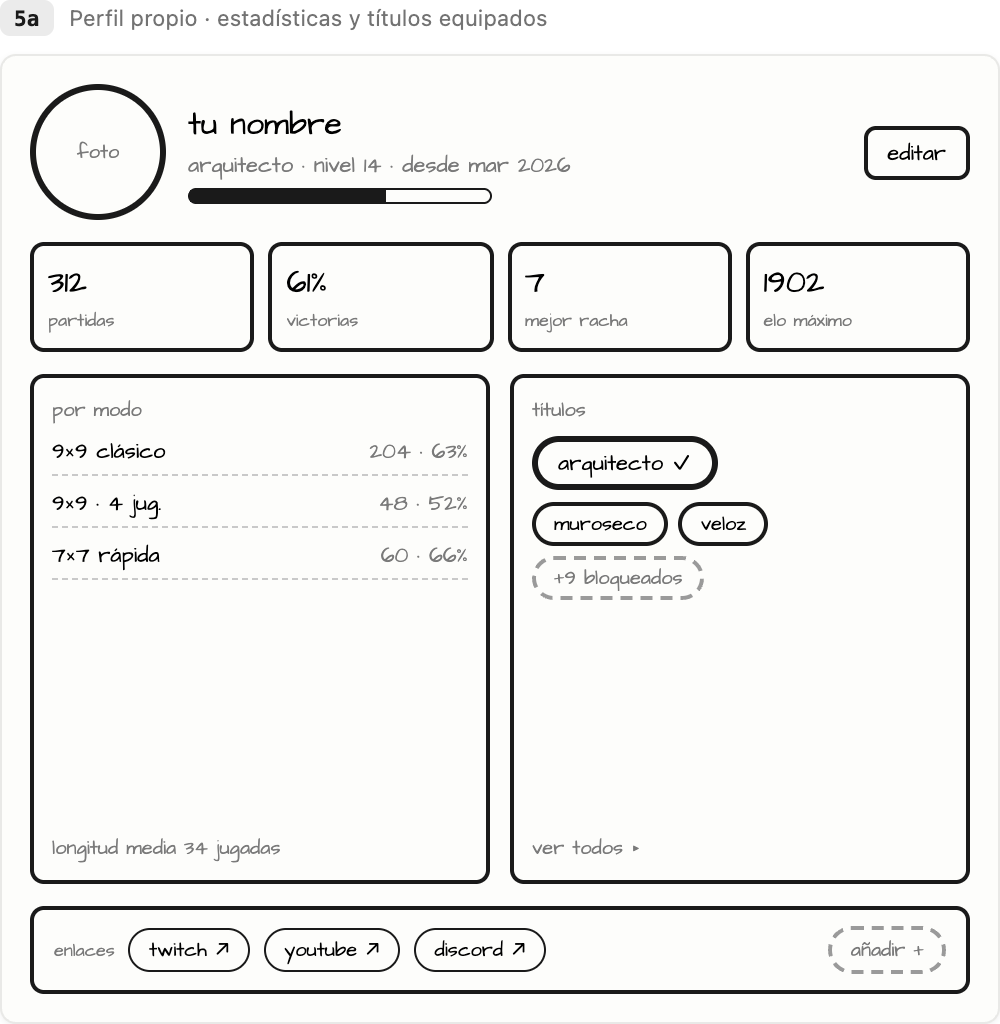
\includegraphics[width=\linewidth]{Prototipos/5a}\par\smallskip
{\footnotesize\textit{Prototipo 5a: Perfil propio · estadísticas y títulos}}
\end{minipage}\hfill
\begin{minipage}[t]{0.48\textwidth}\centering
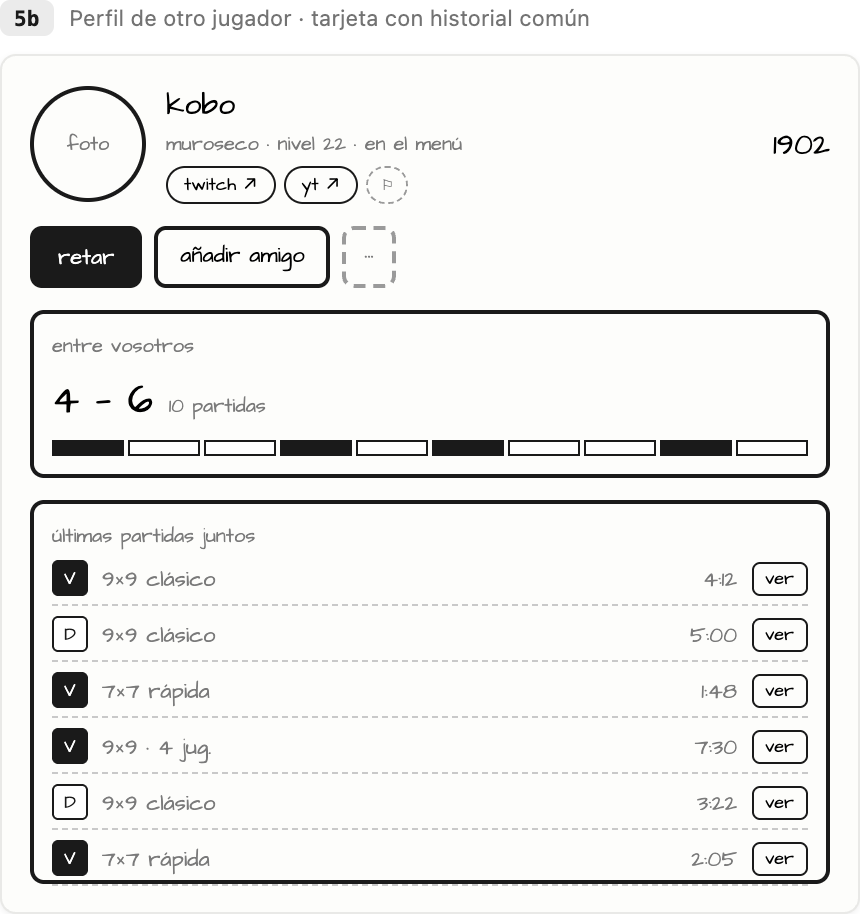
\includegraphics[width=\linewidth]{Prototipos/5b}\par\smallskip
{\footnotesize\textit{Prototipo 5b: Perfil de otro jugador · historial común}}
\end{minipage}
\par\medskip
\begin{minipage}[t]{0.50\textwidth}\centering
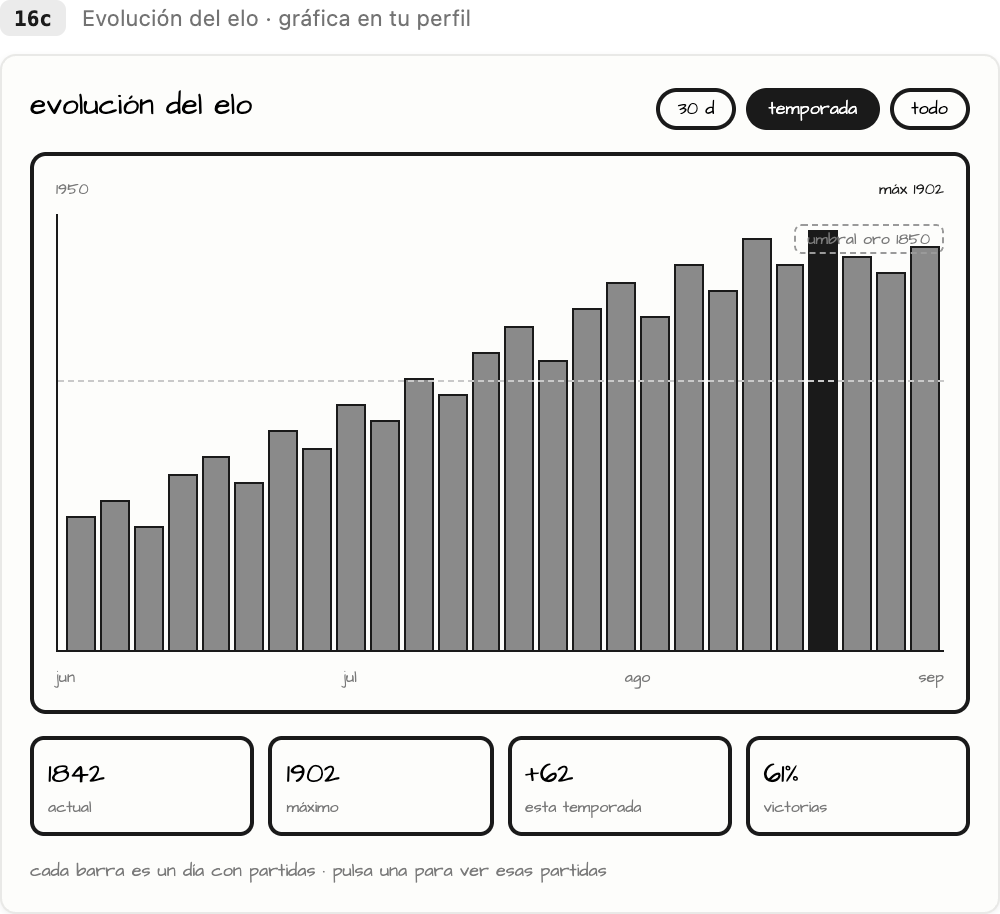
\includegraphics[width=\linewidth]{Prototipos/16c}\par\smallskip
{\footnotesize\textit{Prototipo 16c: Evolución del elo}}
\end{minipage}
\par\medskip
\end{center}

%--- F-07 Editar perfil
\begin{prototipocrud}{F-07}{Editar perfil}
  \crudFila{Operación}{Actualización (U), Creación (C), Eliminación (D)}
  \crudFila{Caso de uso}{\mbox{CU-12}}
  \crudFila{Actor}{Jugador}
  \crudFila{Prototipos}{9c, Editar perfil · foto, nombre y título; 12c, Ajustes · idioma.}
  \crudFila{Datos de entrada}{\begin{crudlista}
    \item \texttt{id\_\allowbreak{}icono}: entero de 1 a 32, o bien una imagen jpg o png de hasta 2 MB.
    \item \texttt{id\_\allowbreak{}objeto} del título a equipar.
    \item Hasta cuatro direcciones web de redes sociales.
    \item \texttt{idioma\_\allowbreak{}preferido}.
    \item Token de sesión.
  \end{crudlista}}
  \crudFila{Datos que se consultan}{\begin{crudlista}
    \item \textit{UsuarioObjeto}: que el título elegido lo posea el usuario.
    \item Catálogo de idiomas admitidos.
  \end{crudlista}}
  \crudFila{Datos que se crean}{\begin{crudlista}
    \item \textit{EnlaceRed}: \texttt{url} y \texttt{orden} de cada enlace nuevo.
    \item \textit{Avatar}: \texttt{ruta\_\allowbreak{}imagen}, \texttt{formato}, \texttt{tamano\_\allowbreak{}bytes}, \texttt{fecha\_\allowbreak{}subida}, \texttt{vigente} = 1, si se subió imagen.
  \end{crudlista}}
  \crudFila{Datos que se modifican}{\begin{crudlista}
    \item \textit{Usuario}: \texttt{id\_\allowbreak{}icono}, \texttt{idioma\_\allowbreak{}preferido}.
    \item \textit{Equipamiento}: la fila de la ranura de título.
    \item \textit{Avatar} anterior: \texttt{vigente} = 0.
  \end{crudlista}}
  \crudFila{Datos que se eliminan}{\begin{crudlista}
    \item \textit{EnlaceRed}: los que el jugador quitó. Borrado físico.
  \end{crudlista}}
  \crudFila{Reglas de negocio}{\begin{crudlista}
    \item El \texttt{nickname} no se modifica aquí (\mbox{CU-12} \mbox{RN-01}).
    \item Máximo cuatro enlaces y ninguno de un acortador (\mbox{CU-12} \mbox{RN-03}, \mbox{RN-04}).
    \item Un solo avatar vigente por usuario (\mbox{CU-12} \mbox{RN-06}).
    \item El título debe poseerse (\mbox{CU-14} \mbox{RN-02}).
    \item Avatar y enlaces se publican sin revisión (\mbox{D-08}).
  \end{crudlista}}
  \crudFila{Resultado esperado}{El perfil muestra el icono o avatar, el título, los enlaces y el idioma elegidos. La identidad de acceso no cambió.}
\end{prototipocrud}
\par\nopagebreak\smallskip
\begin{center}
\begin{minipage}[t]{0.48\textwidth}\centering
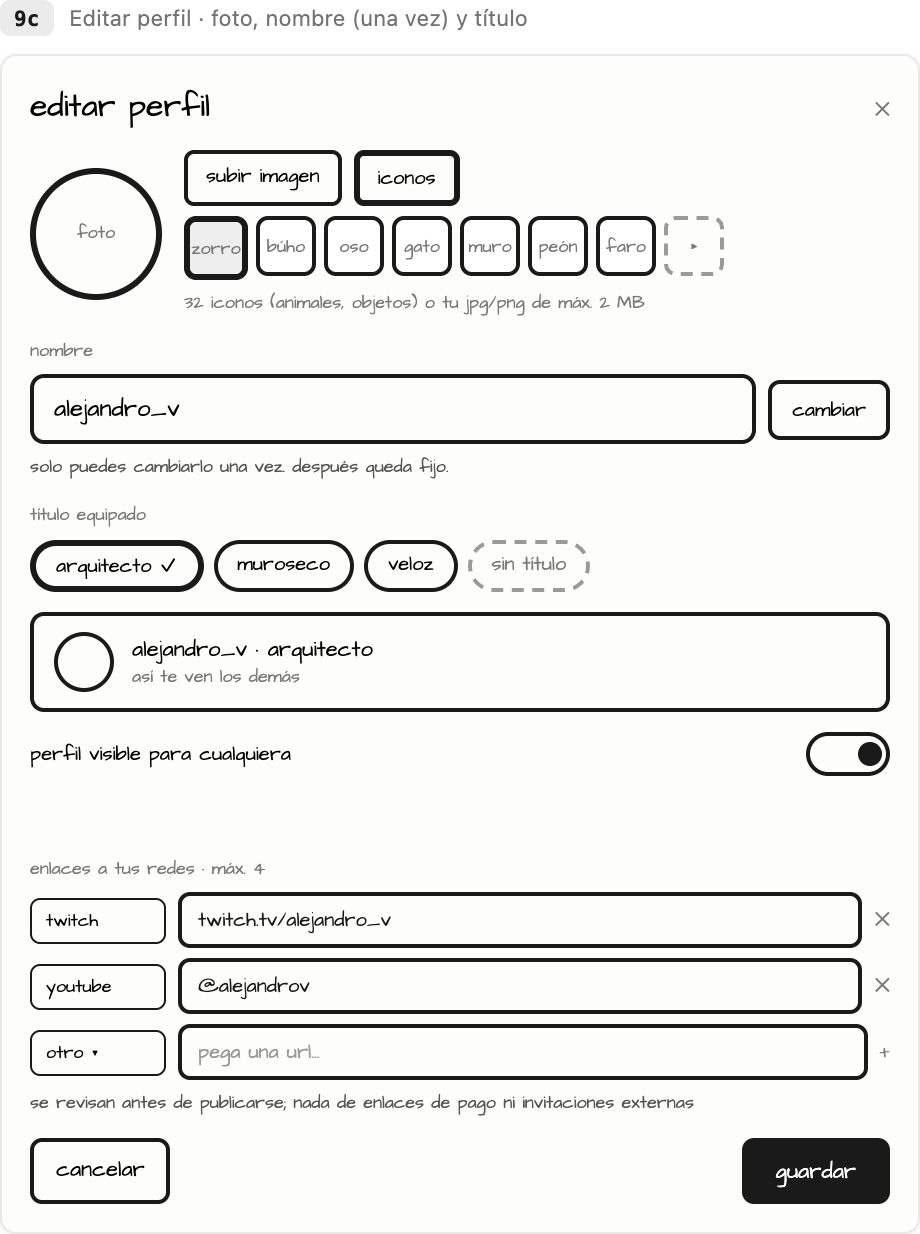
\includegraphics[width=\linewidth]{Prototipos/9c}\par\smallskip
{\footnotesize\textit{Prototipo 9c: Editar perfil · foto, nombre y título}}
\end{minipage}\hfill
\begin{minipage}[t]{0.48\textwidth}\centering
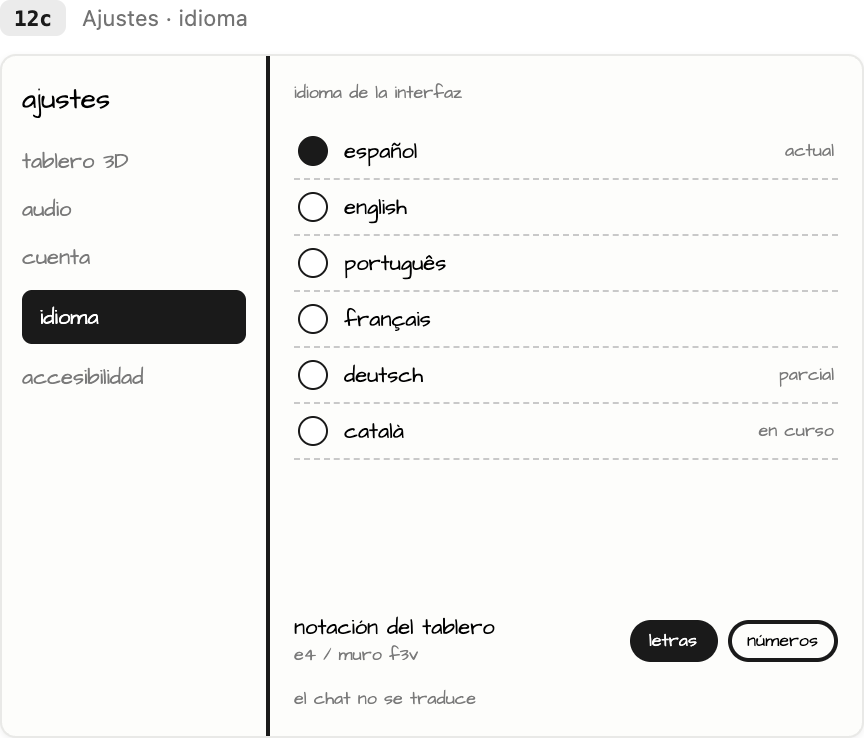
\includegraphics[width=\linewidth]{Prototipos/12c}\par\smallskip
{\footnotesize\textit{Prototipo 12c: Ajustes · idioma}}
\end{minipage}
\par\medskip
\end{center}

%--- F-08 Cambiar nickname
\begin{prototipocrud}{F-08}{Cambiar nickname}
  \crudFila{Operación}{Actualización (U)}
  \crudFila{Caso de uso}{\mbox{CU-13}}
  \crudFila{Actor}{Jugador con cuenta registrada}
  \crudFila{Prototipos}{9d, Cambio de nombre · confirmación.}
  \crudFila{Datos de entrada}{\begin{crudlista}
    \item \texttt{nickname} nuevo: texto de 3 a 30 caracteres.
    \item Confirmación explícita del cambio.
    \item Token de sesión.
  \end{crudlista}}
  \crudFila{Datos que se consultan}{\begin{crudlista}
    \item \textit{HistorialNickname}: si el usuario ya cambió su nombre.
    \item \textit{Usuario}: \texttt{nickname} de las demás cuentas.
    \item \textit{PalabraProhibida}.
  \end{crudlista}}
  \crudFila{Datos que se crean}{\begin{crudlista}
    \item \textit{HistorialNickname}: \texttt{nickname\_\allowbreak{}anterior}, \texttt{nickname\_\allowbreak{}nuevo}, \texttt{fecha\_\allowbreak{}cambio}.
  \end{crudlista}}
  \crudFila{Datos que se modifican}{\begin{crudlista}
    \item \textit{Usuario}: \texttt{nickname}.
  \end{crudlista}}
  \crudFila{Datos que se eliminan}{Ninguno.}
  \crudFila{Reglas de negocio}{\begin{crudlista}
    \item El nombre se cambia una sola vez por cuenta (\mbox{CU-13} \mbox{RN-01}).
    \item Las cuentas de invitado no pueden hacerlo (\mbox{CU-13} \mbox{RN-06}).
    \item El historial y el cambio se escriben en la misma transacción (\mbox{CU-13} \mbox{RN-04}).
    \item Un intento fallido no gasta el cambio (\mbox{CU-13} \mbox{RN-05}).
  \end{crudlista}}
  \crudFila{Resultado esperado}{El jugador tiene su nombre nuevo, el cambio queda registrado y la opción aparece deshabilitada.}
\end{prototipocrud}
\par\nopagebreak\smallskip
\begin{center}
\begin{minipage}[t]{0.50\textwidth}\centering
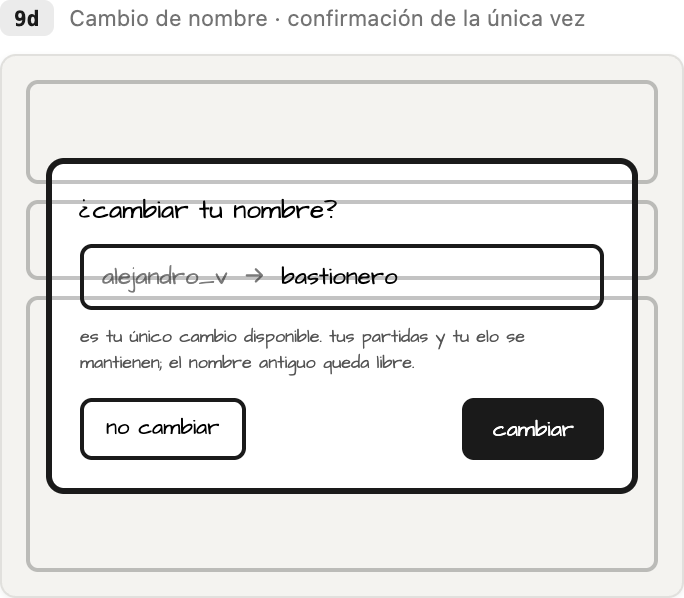
\includegraphics[width=\linewidth]{Prototipos/9d}\par\smallskip
{\footnotesize\textit{Prototipo 9d: Cambio de nombre · confirmación}}
\end{minipage}
\par\medskip
\end{center}

%--- F-09 Recuperar contraseña
\begin{prototipocrud}{F-09}{Recuperar contraseña}
  \crudFila{Operación}{Actualización (U)}
  \crudFila{Caso de uso}{\mbox{CU-03}}
  \crudFila{Actor}{Jugador}
  \crudFila{Prototipos}{9a, Recuperar contraseña · pedir el correo; 9b, Recuperar contraseña · nueva contraseña.}
  \crudFila{Datos de entrada}{\begin{crudlista}
    \item \texttt{correo} de la cuenta.
    \item Código recibido por correo.
    \item Contraseña nueva y su confirmación.
  \end{crudlista}}
  \crudFila{Datos que se consultan}{\begin{crudlista}
    \item \textit{Usuario}: \texttt{correo}, \texttt{estado\_\allowbreak{}cuenta}, \texttt{contrasena\_\allowbreak{}hash}, \texttt{fecha\_\allowbreak{}ultimo\_\allowbreak{}envio\_\allowbreak{}recuperacion}, \texttt{idioma\_\allowbreak{}preferido}.
    \item \textit{TokenRecuperacion}: \texttt{token\_\allowbreak{}hash}, \texttt{usado}, \texttt{intentos}, \texttt{fecha\_\allowbreak{}expiracion}.
  \end{crudlista}}
  \crudFila{Datos que se crean}{\begin{crudlista}
    \item \textit{TokenRecuperacion}: \texttt{token\_\allowbreak{}hash}, \texttt{fecha\_\allowbreak{}expiracion}, \texttt{intentos} = 0, \texttt{usado} = 0.
    \item \textit{BitacoraAcceso}: \texttt{RECUPERACION\_\allowbreak{}SOLICITADA} y \texttt{RECUPERACION\_\allowbreak{}EXITOSA}.
  \end{crudlista}}
  \crudFila{Datos que se modifican}{\begin{crudlista}
    \item \textit{Usuario}: \texttt{contrasena\_\allowbreak{}hash}, \texttt{contrasena\_\allowbreak{}sal}, \texttt{fecha\_\allowbreak{}ultimo\_\allowbreak{}envio\_\allowbreak{}recuperacion}; \texttt{intentos\_\allowbreak{}fallidos} = 0 y \texttt{bloqueada\_\allowbreak{}hasta} en nulo.
    \item \textit{TokenRecuperacion}: \texttt{intentos}, \texttt{usado}.
    \item \textit{Sesion}: todas las abiertas reciben \texttt{fecha\_\allowbreak{}fin} y \texttt{motivo\_\allowbreak{}cierre} = \texttt{CAMBIO\_\allowbreak{}CREDENCIALES}.
  \end{crudlista}}
  \crudFila{Datos que se eliminan}{Ninguno.}
  \crudFila{Reglas de negocio}{\begin{crudlista}
    \item La respuesta es idéntica exista o no la cuenta (\mbox{CU-03} \mbox{RN-01}).
    \item El código vale treinta minutos, es de un solo uso y admite tres intentos (\mbox{CU-03} \mbox{RN-04}, \mbox{RN-09}).
    \item El correo puede pedirse a lo sumo cada cinco minutos (\mbox{CU-03} \mbox{RN-06}).
    \item Recuperar la contraseña cierra todas las sesiones (\mbox{CU-03} \mbox{RN-07}).
  \end{crudlista}}
  \crudFila{Resultado esperado}{La cuenta tiene una contraseña nueva, cualquier bloqueo temporal quedó levantado y ningún dispositivo conserva sesión abierta.}
\end{prototipocrud}
\par\nopagebreak\smallskip
\begin{center}
\begin{minipage}[t]{0.48\textwidth}\centering
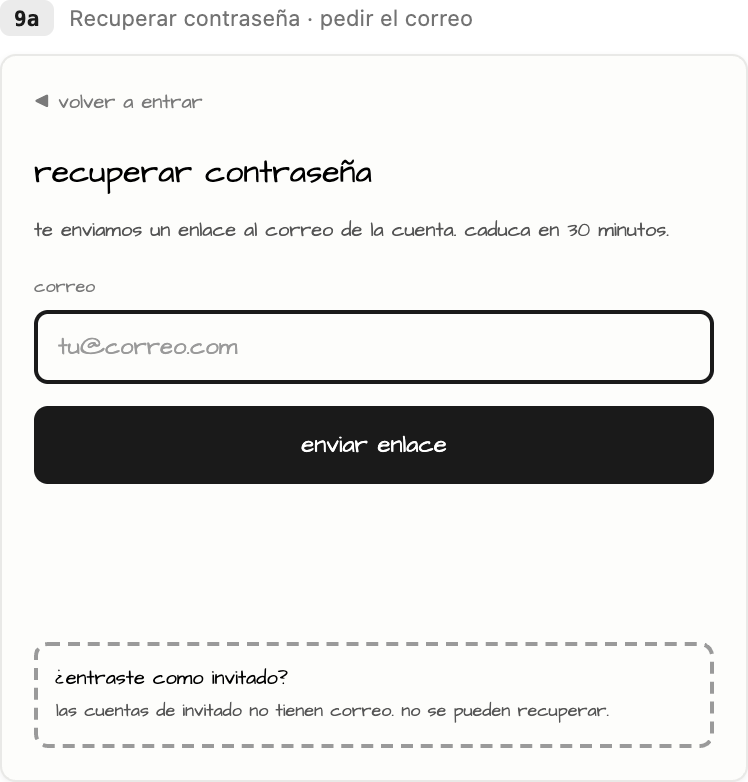
\includegraphics[width=\linewidth]{Prototipos/9a}\par\smallskip
{\footnotesize\textit{Prototipo 9a: Recuperar contraseña · pedir el correo}}
\end{minipage}\hfill
\begin{minipage}[t]{0.48\textwidth}\centering
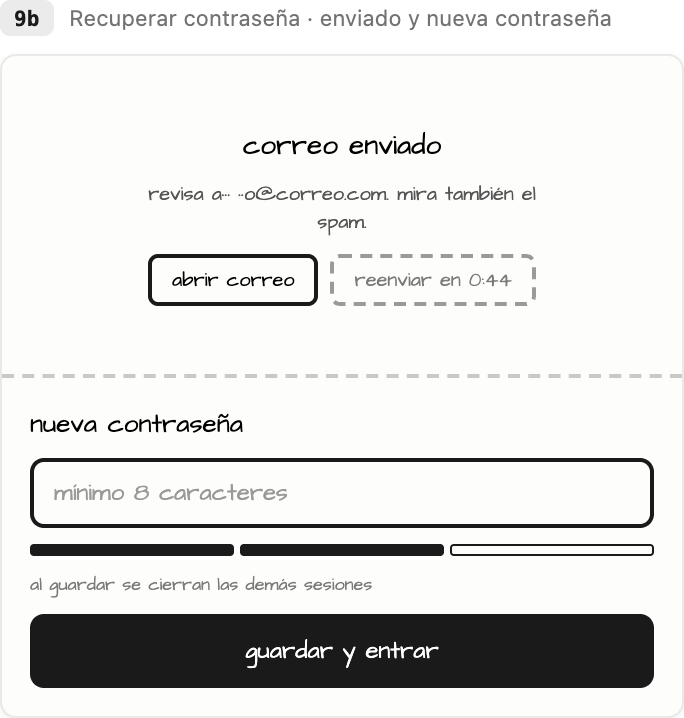
\includegraphics[width=\linewidth]{Prototipos/9b}\par\smallskip
{\footnotesize\textit{Prototipo 9b: Recuperar contraseña · nueva contraseña}}
\end{minipage}
\par\medskip
\end{center}

%--- F-10 Cambiar contraseña
\begin{prototipocrud}{F-10}{Cambiar contraseña}
  \crudFila{Operación}{Actualización (U)}
  \crudFila{Caso de uso}{\mbox{CU-09}}
  \crudFila{Actor}{Jugador con cuenta registrada}
  \crudFila{Prototipos}{9f, Ajustes de cuenta · sesión y baja.}
  \crudFila{Datos de entrada}{\begin{crudlista}
    \item Contraseña actual.
    \item Contraseña nueva y su confirmación: al menos 8 caracteres.
    \item Token de sesión.
  \end{crudlista}}
  \crudFila{Datos que se consultan}{\begin{crudlista}
    \item \textit{Usuario}: \texttt{contrasena\_\allowbreak{}hash}, \texttt{contrasena\_\allowbreak{}sal}, \texttt{correo}.
  \end{crudlista}}
  \crudFila{Datos que se crean}{\begin{crudlista}
    \item \textit{BitacoraAcceso}: \texttt{CAMBIO\_\allowbreak{}CONTRASENA}, o \texttt{CONTRASENA\_\allowbreak{}INCORRECTA} si la actual no coincide.
  \end{crudlista}}
  \crudFila{Datos que se modifican}{\begin{crudlista}
    \item \textit{Usuario}: \texttt{contrasena\_\allowbreak{}hash} y \texttt{contrasena\_\allowbreak{}sal}; si la actual es incorrecta, \texttt{intentos\_\allowbreak{}fallidos}, \texttt{fecha\_\allowbreak{}ultimo\_\allowbreak{}intento\_\allowbreak{}fallido} y \texttt{bloqueada\_\allowbreak{}hasta}.
    \item \textit{Sesion}: todas las abiertas salvo la que hace el cambio reciben \texttt{fecha\_\allowbreak{}fin} y \texttt{motivo\_\allowbreak{}cierre} = \texttt{CAMBIO\_\allowbreak{}CREDENCIALES}.
    \item \textit{TokenRecuperacion}: los pendientes quedan invalidados.
  \end{crudlista}}
  \crudFila{Datos que se eliminan}{Ninguno.}
  \crudFila{Reglas de negocio}{\begin{crudlista}
    \item Exige la contraseña actual aunque haya sesión abierta (\mbox{CU-09} \mbox{RN-01}).
    \item Cierra las demás sesiones pero conserva la actual (\mbox{CU-09} \mbox{RN-04}).
    \item Una contraseña actual incorrecta cuenta para el bloqueo escalonado (\mbox{CU-09} \mbox{RN-09}).
    \item El cambio se avisa al correo de la cuenta, fuera de la transacción (\mbox{CU-09} \mbox{RN-05}).
  \end{crudlista}}
  \crudFila{Resultado esperado}{La cuenta tiene una contraseña nueva y solo sigue abierta la sesión desde la que se cambió.}
\end{prototipocrud}
\par\nopagebreak\smallskip
\begin{center}
\begin{minipage}[t]{0.50\textwidth}\centering
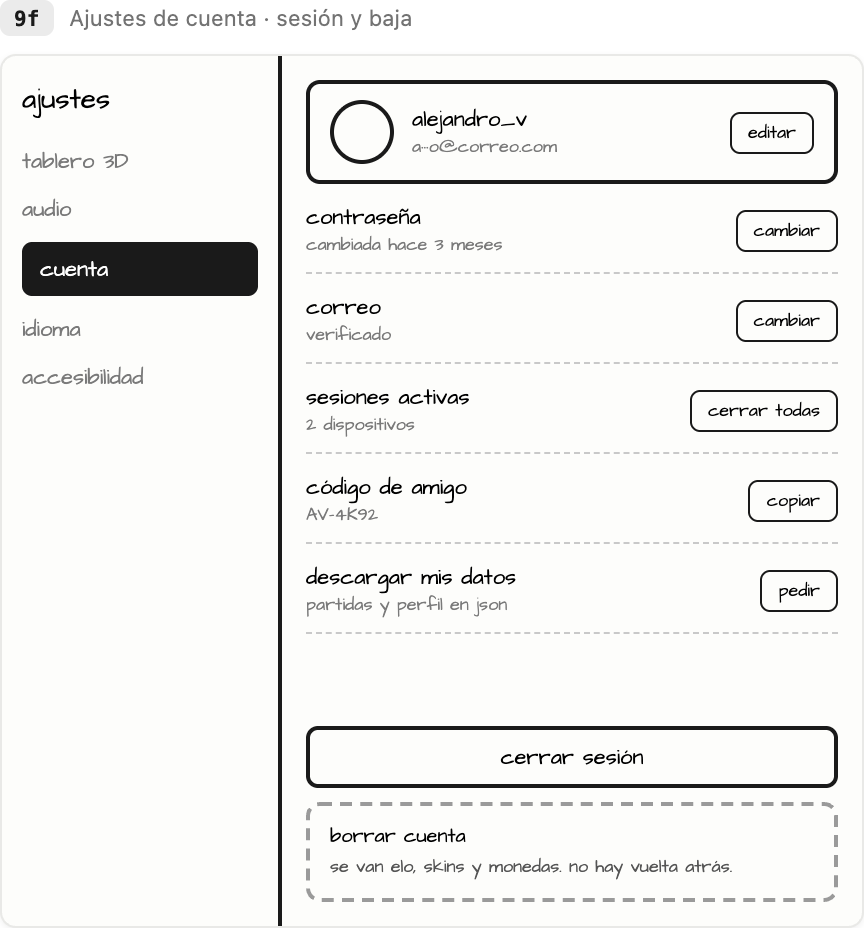
\includegraphics[width=\linewidth]{Prototipos/9f}\par\smallskip
{\footnotesize\textit{Prototipo 9f: Ajustes de cuenta · sesión y baja}}
\end{minipage}
\par\medskip
\end{center}

%--- F-11 Cambiar correo
\begin{prototipocrud}{F-11}{Cambiar correo}
  \crudFila{Operación}{Actualización (U)}
  \crudFila{Caso de uso}{\mbox{CU-09}, \mbox{CU-04}}
  \crudFila{Actor}{Jugador con cuenta registrada}
  \crudFila{Prototipos}{9f, la fila de correo (\mbox{F-10}).}
  \crudFila{Datos de entrada}{\begin{crudlista}
    \item Correo nuevo: hasta 254 caracteres con formato de correo.
    \item Contraseña actual.
    \item Token de sesión; después, el token del enlace enviado al correo nuevo.
  \end{crudlista}}
  \crudFila{Datos que se consultan}{\begin{crudlista}
    \item \textit{Usuario}: \texttt{contrasena\_\allowbreak{}hash}, \texttt{correo} de todas las cuentas, \texttt{fecha\_\allowbreak{}ultimo\_\allowbreak{}envio\_\allowbreak{}verificacion}.
    \item \textit{TokenVerificacionCorreo}: el de \texttt{proposito} = \texttt{CAMBIO\_\allowbreak{}CORREO}, al confirmar.
  \end{crudlista}}
  \crudFila{Datos que se crean}{\begin{crudlista}
    \item \textit{TokenVerificacionCorreo}: \texttt{proposito} = \texttt{CAMBIO\_\allowbreak{}CORREO}, \texttt{correo\_\allowbreak{}destino}, \texttt{token\_\allowbreak{}hash}, \texttt{fecha\_\allowbreak{}expiracion}.
    \item \textit{BitacoraAcceso}: \texttt{CAMBIO\_\allowbreak{}CORREO\_\allowbreak{}SOLICITADO} y \texttt{CAMBIO\_\allowbreak{}CORREO\_\allowbreak{}CONFIRMADO}.
  \end{crudlista}}
  \crudFila{Datos que se modifican}{\begin{crudlista}
    \item \textit{Usuario}: \texttt{fecha\_\allowbreak{}ultimo\_\allowbreak{}envio\_\allowbreak{}verificacion} al solicitar; \texttt{correo} al confirmar.
    \item \textit{TokenVerificacionCorreo}: los pendientes quedan invalidados al solicitar; el usado se marca al confirmar.
  \end{crudlista}}
  \crudFila{Datos que se eliminan}{Ninguno.}
  \crudFila{Reglas de negocio}{\begin{crudlista}
    \item El correo vigente no se sustituye hasta confirmar el nuevo (\mbox{CU-09} \mbox{RN-07}).
    \item Se avisa al correo actual y se confirma desde el nuevo (\mbox{CU-09} \mbox{RN-06}).
    \item El correo pendiente vive en el token, no en \textit{Usuario} (\mbox{D-20}).
    \item Cambiar el correo no devuelve la cuenta a \texttt{PENDIENTE} (\mbox{CU-09} \mbox{POST-04}).
  \end{crudlista}}
  \crudFila{Resultado esperado}{Tras abrir el enlace, la cuenta tiene el correo nuevo; hasta entonces, el anterior sigue vigente y el nuevo aparece como pendiente.}
\end{prototipocrud}

%--- F-12 Eliminar cuenta
\begin{prototipocrud}{F-12}{Eliminar cuenta}
  \crudFila{Operación}{Eliminación (D)}
  \crudFila{Caso de uso}{\mbox{CU-11}}
  \crudFila{Actor}{Jugador con cuenta registrada}
  \crudFila{Prototipos}{9g, Borrar cuenta · confirmación en dos pasos.}
  \crudFila{Datos de entrada}{\begin{crudlista}
    \item Contraseña actual, como primer paso de confirmación.
    \item La palabra de confirmación escrita, como segundo paso.
    \item Token de sesión.
  \end{crudlista}}
  \crudFila{Datos que se consultan}{\begin{crudlista}
    \item \textit{Usuario}: \texttt{contrasena\_\allowbreak{}hash}, \texttt{contrasena\_\allowbreak{}sal}, \texttt{rol}.
    \item \textit{Participacion}: que no haya ninguna sin terminar en una partida en línea.
  \end{crudlista}}
  \crudFila{Datos que se crean}{\begin{crudlista}
    \item \textit{BitacoraAcceso}: \texttt{CUENTA\_\allowbreak{}ELIMINADA} y, a los catorce días, \texttt{CUENTA\_\allowbreak{}ANONIMIZADA}.
  \end{crudlista}}
  \crudFila{Datos que se modifican}{\begin{crudlista}
    \item \textit{Usuario}: \texttt{estado\_\allowbreak{}cuenta} = \texttt{ELIMINADA} y \texttt{fecha\_\allowbreak{}baja}; a los catorce días, \texttt{nickname} y \texttt{correo} anónimos y contraseña en nulo.
    \item \textit{Sesion}: todas las abiertas reciben \texttt{fecha\_\allowbreak{}fin} y \texttt{motivo\_\allowbreak{}cierre} = \texttt{BAJA\_\allowbreak{}CUENTA}.
    \item \textit{Invitacion}: las pendientes pasan a \texttt{EXPIRADA}.
    \item \textit{Reporte}: los que tuviera en revisión como moderador vuelven a \texttt{PENDIENTE}.
    \item \textit{Avatar}: \texttt{vigente} = 0 al anonimizar.
  \end{crudlista}}
  \crudFila{Datos que se eliminan}{\begin{crudlista}
    \item Al darse de baja: su fila de \textit{ColaEmparejamiento} y de \textit{SalaParticipante}, y sus \textit{Solicitud} pendientes.
    \item Al anonimizar: sus \textit{EnlaceRed}, \textit{Amistad}, \textit{Silencio} y \textit{Bloqueo}.
    \item La fila de \textit{Usuario} nunca se elimina (\mbox{D-07}).
  \end{crudlista}}
  \crudFila{Reglas de negocio}{\begin{crudlista}
    \item La baja exige confirmación en dos pasos (\mbox{CU-11} \mbox{RN-01}).
    \item Es recuperable durante catorce días desde \texttt{fecha\_\allowbreak{}baja} (\mbox{CU-11} \mbox{RN-02}, \mbox{D-17}).
    \item Pasado el plazo se anonimiza en lugar de eliminarse (\mbox{CU-11} \mbox{RN-03}).
    \item No puede darse de baja una cuenta con partida en curso ni una de administración (\mbox{CU-11} \mbox{RN-04}, \mbox{RN-06}).
    \item Partidas, jugadas, mensajes, reportes y sanciones se conservan (\mbox{CU-11} \mbox{RN-05}).
  \end{crudlista}}
  \crudFila{Resultado esperado}{La cuenta queda \texttt{ELIMINADA}, sin sesiones abiertas y fuera del ranking, y puede recuperarse durante catorce días; después se anonimiza.}
\end{prototipocrud}
\par\nopagebreak\smallskip
\begin{center}
\begin{minipage}[t]{0.50\textwidth}\centering
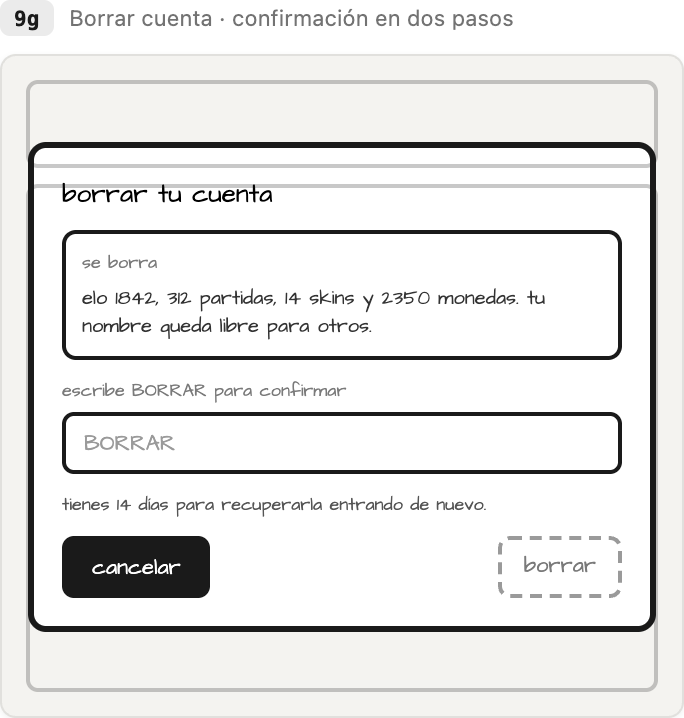
\includegraphics[width=\linewidth]{Prototipos/9g}\par\smallskip
{\footnotesize\textit{Prototipo 9g: Borrar cuenta · confirmación en dos pasos}}
\end{minipage}
\par\medskip
\end{center}

%--- F-13 Recuperar una cuenta eliminada
\begin{prototipocrud}{F-13}{Recuperar una cuenta eliminada}
  \crudFila{Operación}{Actualización (U)}
  \crudFila{Caso de uso}{\mbox{CU-01} (\mbox{FA-17})}
  \crudFila{Actor}{Jugador}
  \crudFila{Prototipos}{Sin prototipo.}
  \crudFila{Datos de entrada}{\begin{crudlista}
    \item Identificador y contraseña, como en el inicio de sesión.
    \item Confirmación de que desea recuperar la cuenta.
  \end{crudlista}}
  \crudFila{Datos que se consultan}{\begin{crudlista}
    \item \textit{Usuario}: \texttt{estado\_\allowbreak{}cuenta}, \texttt{fecha\_\allowbreak{}baja}, \texttt{contrasena\_\allowbreak{}hash}, \texttt{contrasena\_\allowbreak{}sal}.
  \end{crudlista}}
  \crudFila{Datos que se crean}{\begin{crudlista}
    \item \textit{BitacoraAcceso}: \texttt{resultado} = \texttt{CUENTA\_\allowbreak{}RECUPERADA}.
    \item \textit{Sesion}: la que se abre al continuar el inicio de sesión.
  \end{crudlista}}
  \crudFila{Datos que se modifican}{\begin{crudlista}
    \item \textit{Usuario}: \texttt{estado\_\allowbreak{}cuenta} vuelve a \texttt{ACTIVA} y \texttt{fecha\_\allowbreak{}baja} queda en nulo.
  \end{crudlista}}
  \crudFila{Datos que se eliminan}{Ninguno.}
  \crudFila{Reglas de negocio}{\begin{crudlista}
    \item Solo es posible dentro de los catorce días siguientes a \texttt{fecha\_\allowbreak{}baja} (\mbox{CU-01} \mbox{RN-15}).
    \item Pasado el plazo, la cuenta se trata como inexistente (\mbox{CU-01} \mbox{FA-17}).
    \item La recuperación no restaura las solicitudes ni la cola que se eliminaron al darse de baja.
  \end{crudlista}}
  \crudFila{Resultado esperado}{La cuenta vuelve a estar activa, con su progreso intacto, y el jugador entra al menú principal.}
\end{prototipocrud}

\subsection*{Sesión}
\addcontentsline{toc}{subsection}{Sesión}

Una cuenta puede tener varias sesiones abiertas, una por dispositivo (\mbox{D-01}). La sesión no se borra al cerrarse: queda registrada con su fecha y su motivo de cierre.

%--- F-14 Iniciar sesión
\begin{prototipocrud}{F-14}{Iniciar sesión}
  \crudFila{Operación}{Creación (C)}
  \crudFila{Caso de uso}{\mbox{CU-01}}
  \crudFila{Actor}{Jugador}
  \crudFila{Prototipos}{6c, Inicio de sesión; 3b, Menú principal · tablero 3D de fondo.}
  \crudFila{Datos de entrada}{\begin{crudlista}
    \item Identificador: \texttt{nickname} o \texttt{correo}.
    \item Contraseña.
    \item Código del segundo factor, si la cuenta lo tiene habilitado.
    \item Huella del dispositivo y \texttt{version\_\allowbreak{}cliente}.
  \end{crudlista}}
  \crudFila{Datos que se consultan}{\begin{crudlista}
    \item \textit{Usuario}: \texttt{nickname}, \texttt{correo}, \texttt{tipo\_\allowbreak{}cuenta}, \texttt{contrasena\_\allowbreak{}hash}, \texttt{contrasena\_\allowbreak{}sal}, \texttt{estado\_\allowbreak{}cuenta}, \texttt{fecha\_\allowbreak{}baja}, \texttt{bloqueada\_\allowbreak{}hasta}, \texttt{intentos\_\allowbreak{}fallidos}, \texttt{doble\_\allowbreak{}factor\_\allowbreak{}habilitado}, \texttt{idioma\_\allowbreak{}preferido}, \texttt{id\_\allowbreak{}icono}, \texttt{fecha\_\allowbreak{}configuracion\_\allowbreak{}inicial}.
    \item \textit{Sancion}: activas con \texttt{ambito} = \texttt{CUENTA}.
    \item \textit{EstadisticaModo}, \textit{Equipamiento} y la \textit{Participacion} sin terminar, para cargar el menú.
  \end{crudlista}}
  \crudFila{Datos que se crean}{\begin{crudlista}
    \item \textit{Sesion}: \texttt{token\_\allowbreak{}hash}, \texttt{fecha\_\allowbreak{}inicio}, \texttt{fecha\_\allowbreak{}expiracion}, \texttt{direccion\_\allowbreak{}ip}, \texttt{huella\_\allowbreak{}dispositivo}, \texttt{nombre\_\allowbreak{}dispositivo}, \texttt{version\_\allowbreak{}cliente}.
    \item \textit{CodigoSegundoFactor}: \texttt{codigo\_\allowbreak{}hash}, \texttt{fecha\_\allowbreak{}generacion}, \texttt{fecha\_\allowbreak{}expiracion}, \texttt{intentos}, \texttt{consumido}, \texttt{canal}, si aplica.
    \item \textit{TokenVerificacionCorreo}, si una cuenta pendiente pide reenviar el correo.
    \item \textit{BitacoraAcceso}: con el resultado del intento, sea exitoso o no.
  \end{crudlista}}
  \crudFila{Datos que se modifican}{\begin{crudlista}
    \item \textit{Usuario}: \texttt{intentos\_\allowbreak{}fallidos}, \texttt{fecha\_\allowbreak{}ultimo\_\allowbreak{}intento\_\allowbreak{}fallido}, \texttt{bloqueada\_\allowbreak{}hasta}, \texttt{fecha\_\allowbreak{}ultimo\_\allowbreak{}acceso} y, en el reenvío, \texttt{fecha\_\allowbreak{}ultimo\_\allowbreak{}envio\_\allowbreak{}verificacion}.
  \end{crudlista}}
  \crudFila{Datos que se eliminan}{Ninguno.}
  \crudFila{Reglas de negocio}{\begin{crudlista}
    \item Ante credenciales inválidas el mensaje es genérico (\mbox{CU-01} \mbox{RN-01}).
    \item El bloqueo por intentos fallidos es escalonado: 5, 30 y 60 minutos (\mbox{CU-01} \mbox{RN-03}).
    \item Solo inicia sesión una cuenta \texttt{ACTIVA} y sin sanción de cuenta vigente (\mbox{CU-01} \mbox{RN-04}, \mbox{RN-05}).
    \item El token vale veinticuatro horas (\mbox{CU-01} \mbox{RN-07}).
    \item Se permiten varias sesiones simultáneas (\mbox{CU-01} \mbox{RN-06}, \mbox{D-01}).
    \item Los invitados no inician sesión por esta vía (\mbox{CU-01} \mbox{RN-16}).
  \end{crudlista}}
  \crudFila{Resultado esperado}{Existe una sesión abierta para ese dispositivo y el cliente muestra el menú principal, la configuración inicial o la partida en curso, según corresponda.}
\end{prototipocrud}
\par\nopagebreak\smallskip
\begin{center}
\begin{minipage}[t]{0.48\textwidth}\centering
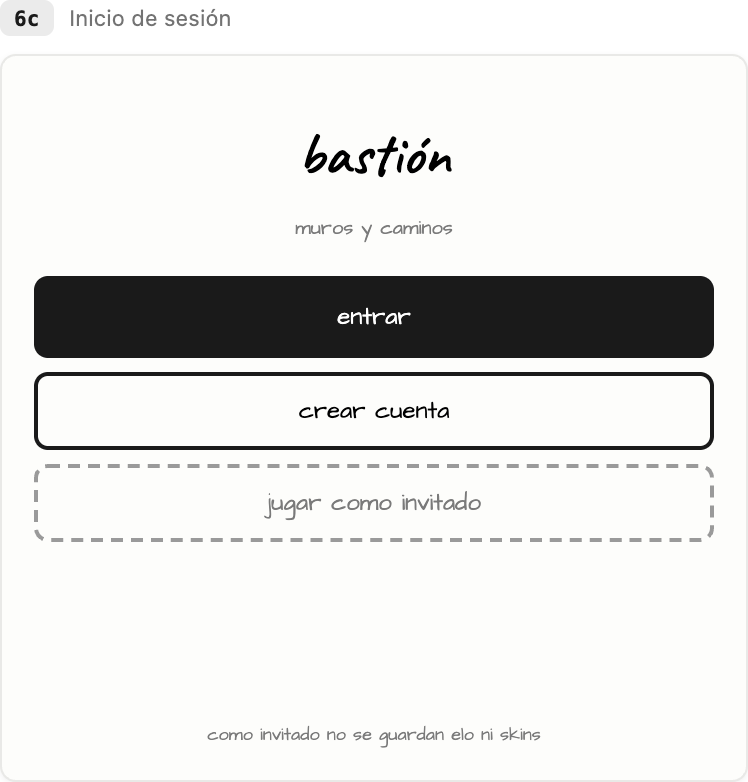
\includegraphics[width=\linewidth]{Prototipos/6c}\par\smallskip
{\footnotesize\textit{Prototipo 6c: Inicio de sesión}}
\end{minipage}\hfill
\begin{minipage}[t]{0.48\textwidth}\centering
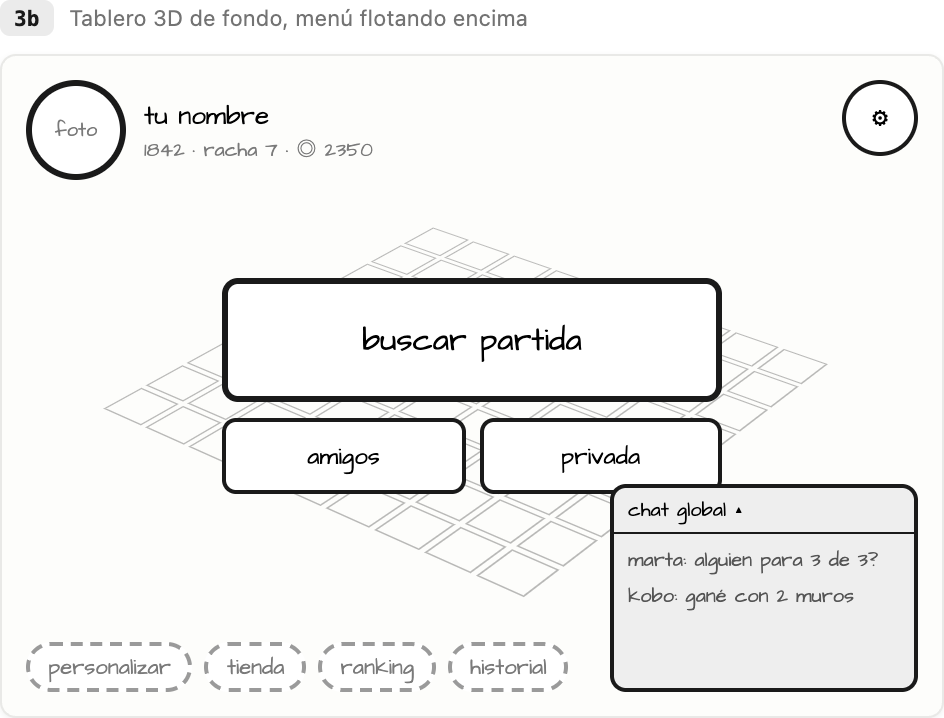
\includegraphics[width=\linewidth]{Prototipos/3b}\par\smallskip
{\footnotesize\textit{Prototipo 3b: Menú principal · tablero 3D de fondo}}
\end{minipage}
\par\medskip
\end{center}

%--- F-15 Consultar sesiones activas
\begin{prototipocrud}{F-15}{Consultar sesiones activas}
  \crudFila{Operación}{Consulta (R)}
  \crudFila{Caso de uso}{\mbox{CU-10}}
  \crudFila{Actor}{Jugador}
  \crudFila{Prototipos}{9f, la fila de sesiones activas (\mbox{F-10}).}
  \crudFila{Datos de entrada}{\begin{crudlista}
    \item Token de sesión.
  \end{crudlista}}
  \crudFila{Datos que se consultan}{\begin{crudlista}
    \item \textit{Sesion}: las del usuario con \texttt{fecha\_\allowbreak{}fin} nula y \texttt{fecha\_\allowbreak{}expiracion} futura; de cada una, \texttt{nombre\_\allowbreak{}dispositivo}, \texttt{direccion\_\allowbreak{}ip}, \texttt{fecha\_\allowbreak{}inicio} y \texttt{fecha\_\allowbreak{}ultimo\_\allowbreak{}uso}.
  \end{crudlista}}
  \crudFila{Datos que se crean}{Ninguno.}
  \crudFila{Datos que se modifican}{Ninguno.}
  \crudFila{Datos que se eliminan}{Ninguno.}
  \crudFila{Reglas de negocio}{\begin{crudlista}
    \item Solo se listan las sesiones propias (\mbox{CU-10} \mbox{RN-01}).
    \item Una sesión expirada no se lista aunque su \texttt{fecha\_\allowbreak{}fin} siga nula (\mbox{CU-10} \mbox{RN-02}).
    \item La dirección de red se muestra parcialmente oculta (\mbox{CU-10} \mbox{RN-03}).
  \end{crudlista}}
  \crudFila{Resultado esperado}{El jugador ve en qué dispositivos tiene sesión abierta, desde cuándo y cuándo se usó por última vez.}
\end{prototipocrud}

%--- F-16 Cerrar sesión
\begin{prototipocrud}{F-16}{Cerrar sesión}
  \crudFila{Operación}{Eliminación (D)}
  \crudFila{Caso de uso}{\mbox{CU-05}, \mbox{CU-10}}
  \crudFila{Actor}{Jugador}
  \crudFila{Prototipos}{9f, las opciones ``cerrar todas'' y ``cerrar sesión'' (\mbox{F-10}).}
  \crudFila{Datos de entrada}{\begin{crudlista}
    \item Token de sesión.
    \item Opcionalmente, \texttt{id\_\allowbreak{}sesion} de otra sesión propia, o la orden de cerrar todas las demás.
  \end{crudlista}}
  \crudFila{Datos que se consultan}{\begin{crudlista}
    \item \textit{Sesion}: la del token y, si aplica, las demás del usuario.
    \item \textit{Participacion}: si hay una partida sin terminar, para advertirlo.
  \end{crudlista}}
  \crudFila{Datos que se crean}{\begin{crudlista}
    \item \textit{BitacoraAcceso}: \texttt{CIERRE\_\allowbreak{}VOLUNTARIO} o \texttt{CIERRE\_\allowbreak{}REMOTO}.
  \end{crudlista}}
  \crudFila{Datos que se modifican}{\begin{crudlista}
    \item \textit{Sesion}: \texttt{fecha\_\allowbreak{}fin} y \texttt{motivo\_\allowbreak{}cierre} = \texttt{CIERRE\_\allowbreak{}VOLUNTARIO} para la propia, o \texttt{CIERRE\_\allowbreak{}REMOTO} para las cerradas desde otro dispositivo.
  \end{crudlista}}
  \crudFila{Datos que se eliminan}{Ninguna fila. La sesión se cierra, no se borra.}
  \crudFila{Reglas de negocio}{\begin{crudlista}
    \item El token se invalida en el servidor, no solo en el cliente (\mbox{CU-05} \mbox{RN-02}).
    \item Cerrar sesión no retira al jugador de una partida en curso (\mbox{CU-05} \mbox{RN-04}, \mbox{CU-10} \mbox{RN-06}).
    \item Cerrar todas las demás conserva la sesión desde la que se ordena (\mbox{CU-10} \mbox{POST-03}).
  \end{crudlista}}
  \crudFila{Resultado esperado}{Las sesiones indicadas quedan cerradas y sus tokens dejan de ser válidos.}
\end{prototipocrud}

\subsection*{Emparejamiento y salas}
\addcontentsline{toc}{subsection}{Emparejamiento y salas}

Hay tres formas de reunir a los jugadores de una partida en línea: la cola clasificatoria, la sala privada con código y la invitación directa, que usa una sala. Todas respetan la regla de una sola participación sin terminar por jugador (\mbox{D-11}).

%--- F-17 Buscar partida clasificatoria
\begin{prototipocrud}{F-17}{Buscar partida clasificatoria}
  \crudFila{Operación}{Creación (C), Eliminación (D)}
  \crudFila{Caso de uso}{\mbox{CU-17}}
  \crudFila{Actor}{Jugador}
  \crudFila{Prototipos}{16a, Elegir modo · pantalla propia; 1g, Emparejamiento · rival encontrado (VS).}
  \crudFila{Datos de entrada}{\begin{crudlista}
    \item \texttt{id\_\allowbreak{}modo}: clásico 9×9, cuatro jugadores o rápida 7×7.
    \item \texttt{minutos\_\allowbreak{}reloj}: 3, 5 o 10.
    \item Token de sesión.
  \end{crudlista}}
  \crudFila{Datos que se consultan}{\begin{crudlista}
    \item \textit{Participacion}: que el jugador no tenga ninguna sin terminar en una partida en línea.
    \item \textit{Sancion}: activas con \texttt{ambito} = \texttt{CUENTA}.
    \item \textit{EstadisticaModo}: \texttt{puntos\_\allowbreak{}elo} del modo elegido.
    \item \textit{ColaEmparejamiento}: candidatos del mismo modo y reloj.
    \item \textit{Bloqueo}: entre los candidatos.
    \item \textit{Modo}: \texttt{tamano\_\allowbreak{}tablero}, \texttt{num\_\allowbreak{}jugadores}, \texttt{muros\_\allowbreak{}por\_\allowbreak{}jugador}.
    \item \textit{Equipamiento} de cada participante.
  \end{crudlista}}
  \crudFila{Datos que se crean}{\begin{crudlista}
    \item \textit{ColaEmparejamiento}: \texttt{id\_\allowbreak{}usuario}, \texttt{id\_\allowbreak{}modo}, \texttt{minutos\_\allowbreak{}reloj}, \texttt{elo}, \texttt{fecha\_\allowbreak{}entrada}.
    \item \textit{Partida}: \texttt{id\_\allowbreak{}modo}, \texttt{minutos\_\allowbreak{}reloj}, \texttt{tipo} = \texttt{CLASIFICATORIA}, \texttt{estado} = \texttt{EN\_\allowbreak{}CURSO}, \texttt{fecha\_\allowbreak{}inicio}, \texttt{turno\_\allowbreak{}actual}.
    \item \textit{Participacion}: una por jugador, con \texttt{orden\_\allowbreak{}turno}, \texttt{simbolo\_\allowbreak{}peon}, \texttt{casilla\_\allowbreak{}actual}, \texttt{muros\_\allowbreak{}restantes}, \texttt{reloj\_\allowbreak{}restante}, \texttt{elo\_\allowbreak{}inicial} y \texttt{conectado} = 1.
    \item \textit{ParticipacionObjeto}: el objeto equipado en cada ranura al empezar.
  \end{crudlista}}
  \crudFila{Datos que se modifican}{\begin{crudlista}
    \item \textit{Partida} contra la IA sin terminar, si la hay: se cierra con \texttt{forma\_\allowbreak{}termino} = \texttt{ABANDONO} (\mbox{D-11}).
  \end{crudlista}}
  \crudFila{Datos que se eliminan}{\begin{crudlista}
    \item \textit{ColaEmparejamiento}: las filas de los jugadores emparejados. Borrado físico.
  \end{crudlista}}
  \crudFila{Reglas de negocio}{\begin{crudlista}
    \item Un jugador no puede tener más de una participación sin terminar (\mbox{CU-17} \mbox{RN-01}, \mbox{D-11}).
    \item El modo fija tablero, jugadores y muros (\mbox{CU-17} \mbox{RN-02}).
    \item La ventana de elo se amplía con la espera (\mbox{CU-17} \mbox{RN-03}).
    \item El elo inicial y el aspecto se fijan en la participación (\mbox{CU-17} \mbox{RN-04}, \mbox{RN-06}).
    \item Dos jugadores con bloqueo no se emparejan (\mbox{CU-17} \mbox{RN-05}).
    \item Partida, participaciones y salida de la cola se escriben en una transacción (\mbox{CU-17} \mbox{RN-10}).
  \end{crudlista}}
  \crudFila{Resultado esperado}{Existe una partida en curso con todos sus participantes y sus aspectos fijados, y los jugadores ya no están en la cola.}
\end{prototipocrud}
\par\nopagebreak\smallskip
\begin{center}
\begin{minipage}[t]{0.48\textwidth}\centering
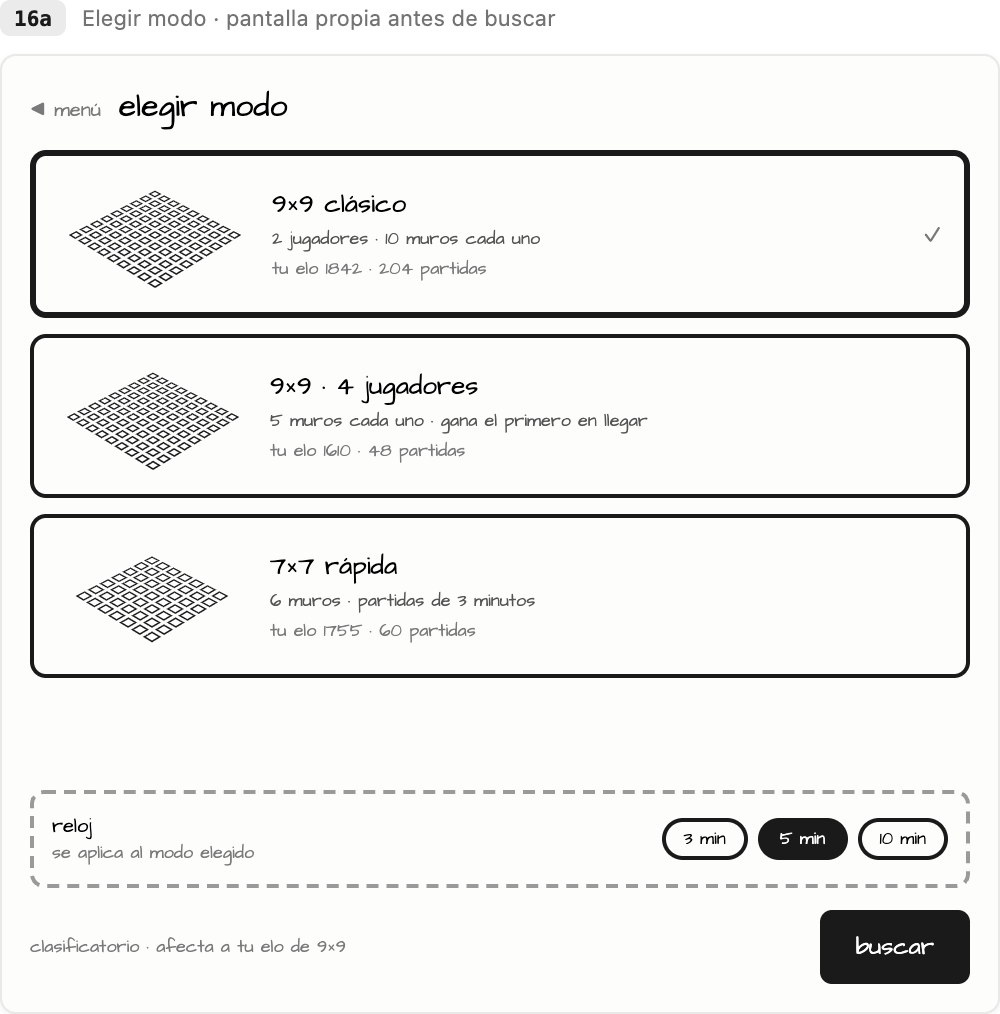
\includegraphics[width=\linewidth]{Prototipos/16a}\par\smallskip
{\footnotesize\textit{Prototipo 16a: Elegir modo · pantalla propia}}
\end{minipage}\hfill
\begin{minipage}[t]{0.48\textwidth}\centering
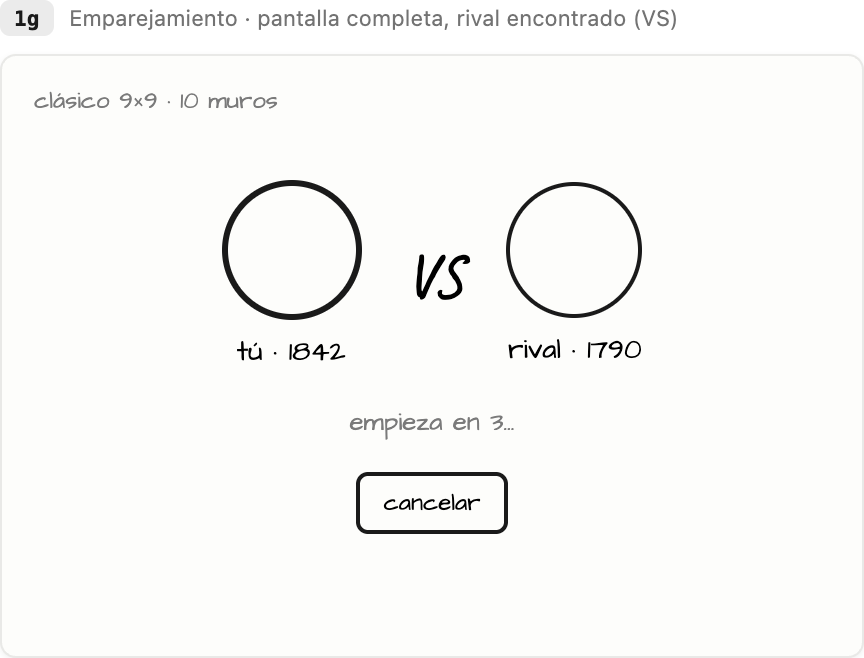
\includegraphics[width=\linewidth]{Prototipos/1g}\par\smallskip
{\footnotesize\textit{Prototipo 1g: Emparejamiento · rival encontrado (VS)}}
\end{minipage}
\par\medskip
\end{center}

%--- F-18 Cancelar búsqueda de partida
\begin{prototipocrud}{F-18}{Cancelar búsqueda de partida}
  \crudFila{Operación}{Eliminación (D)}
  \crudFila{Caso de uso}{\mbox{CU-17} (\mbox{FA-03})}
  \crudFila{Actor}{Jugador}
  \crudFila{Prototipos}{1f, Emparejamiento · modal sobre el menú.}
  \crudFila{Datos de entrada}{\begin{crudlista}
    \item Token de sesión.
  \end{crudlista}}
  \crudFila{Datos que se consultan}{\begin{crudlista}
    \item \textit{ColaEmparejamiento}: la fila del jugador.
  \end{crudlista}}
  \crudFila{Datos que se crean}{Ninguno.}
  \crudFila{Datos que se modifican}{Ninguno.}
  \crudFila{Datos que se eliminan}{\begin{crudlista}
    \item \textit{ColaEmparejamiento}: la fila del jugador. Borrado físico.
  \end{crudlista}}
  \crudFila{Reglas de negocio}{\begin{crudlista}
    \item La cola es transitoria y no conserva historial.
    \item La fila también se elimina si el jugador pierde la conexión (\mbox{CU-17} \mbox{EX-04}).
  \end{crudlista}}
  \crudFila{Resultado esperado}{El jugador sale de la cola sin que se haya creado ninguna partida.}
\end{prototipocrud}
\par\nopagebreak\smallskip
\begin{center}
\begin{minipage}[t]{0.50\textwidth}\centering
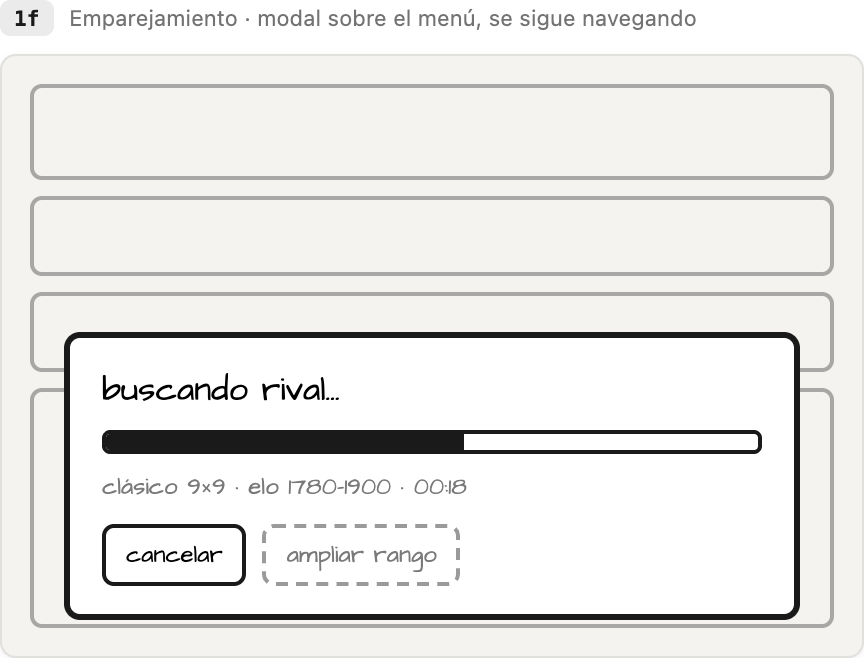
\includegraphics[width=\linewidth]{Prototipos/1f}\par\smallskip
{\footnotesize\textit{Prototipo 1f: Emparejamiento · modal sobre el menú}}
\end{minipage}
\par\medskip
\end{center}

%--- F-19 Crear sala privada e iniciar su partida
\begin{prototipocrud}{F-19}{Crear sala privada e iniciar su partida}
  \crudFila{Operación}{Creación (C), Actualización (U), Eliminación (D)}
  \crudFila{Caso de uso}{\mbox{CU-18}}
  \crudFila{Actor}{Jugador o invitado, como anfitrión}
  \crudFila{Prototipos}{1h, Privada · crear o unirse, con ajustes de sala; 5d, Sala de espera · 2 jugadores.}
  \crudFila{Datos de entrada}{\begin{crudlista}
    \item \texttt{id\_\allowbreak{}modo}.
    \item \texttt{muros\_\allowbreak{}por\_\allowbreak{}jugador}: entero de 1 a 20.
    \item \texttt{minutos\_\allowbreak{}reloj}: 3, 5 o 10.
    \item \texttt{permite\_\allowbreak{}espectadores}: sí o no.
    \item Token de sesión.
  \end{crudlista}}
  \crudFila{Datos que se consultan}{\begin{crudlista}
    \item \textit{Participacion}, \textit{ColaEmparejamiento} y \textit{SalaParticipante}: que el anfitrión no esté en partida, cola ni otra sala.
    \item \textit{Sancion}: activas con \texttt{ambito} = \texttt{CUENTA}.
    \item \textit{Modo}: número de plazas.
    \item \textit{Sala}: códigos en uso entre las abiertas.
    \item \textit{EstadisticaModo} y \textit{Equipamiento} de cada miembro, al iniciar.
  \end{crudlista}}
  \crudFila{Datos que se crean}{\begin{crudlista}
    \item \textit{Sala}: \texttt{codigo}, \texttt{id\_\allowbreak{}anfitrion}, \texttt{id\_\allowbreak{}modo}, \texttt{muros\_\allowbreak{}por\_\allowbreak{}jugador}, \texttt{minutos\_\allowbreak{}reloj}, \texttt{permite\_\allowbreak{}espectadores}, \texttt{estado} = \texttt{ABIERTA}, \texttt{fecha\_\allowbreak{}creacion}.
    \item \textit{SalaParticipante}: la del anfitrión, con \texttt{plaza}, \texttt{listo} = 1 y \texttt{fecha\_\allowbreak{}union}.
    \item \textit{Mensaje}: los del chat de sala, con \texttt{canal} = \texttt{SALA}.
    \item Al iniciar: \textit{Partida} con \texttt{tipo} = \texttt{PRIVADA}, una \textit{Participacion} y su \textit{ParticipacionObjeto} por miembro.
  \end{crudlista}}
  \crudFila{Datos que se modifican}{\begin{crudlista}
    \item \textit{Sala}: ajustes; \texttt{estado} = \texttt{EN\_\allowbreak{}PARTIDA} e \texttt{id\_\allowbreak{}partida} al iniciar; \texttt{estado} = \texttt{CERRADA} si el anfitrión sale o por inactividad.
    \item \textit{SalaParticipante}: \texttt{listo} = 0 de los demás miembros al cambiar los ajustes.
  \end{crudlista}}
  \crudFila{Datos que se eliminan}{\begin{crudlista}
    \item \textit{SalaParticipante}: la de cada miembro que sale y todas al cerrar la sala. Borrado físico.
  \end{crudlista}}
  \crudFila{Reglas de negocio}{\begin{crudlista}
    \item El código tiene seis caracteres sin ambiguos y es único entre las salas abiertas (\mbox{CU-18} \mbox{RN-01}).
    \item Un jugador está en una sola sala abierta, y nunca a la vez en sala y en cola o partida (\mbox{CU-18} \mbox{RN-02}).
    \item Las partidas privadas no otorgan elo ni monedas (\mbox{CU-18} \mbox{RN-03}, \mbox{D-16}).
    \item Solo se inicia con todas las plazas ocupadas y todos listos (\mbox{CU-18} \mbox{RN-05}).
    \item Si el anfitrión sale, la sala se cierra; no se transfiere (\mbox{CU-18} \mbox{RN-07}).
    \item Una sala inactiva treinta minutos se cierra sola (\mbox{CU-18} \mbox{RN-08}).
  \end{crudlista}}
  \crudFila{Resultado esperado}{Existe una partida privada en curso con todos los miembros de la sala, que queda asociada a ella.}
\end{prototipocrud}
\par\nopagebreak\smallskip
\begin{center}
\begin{minipage}[t]{0.48\textwidth}\centering
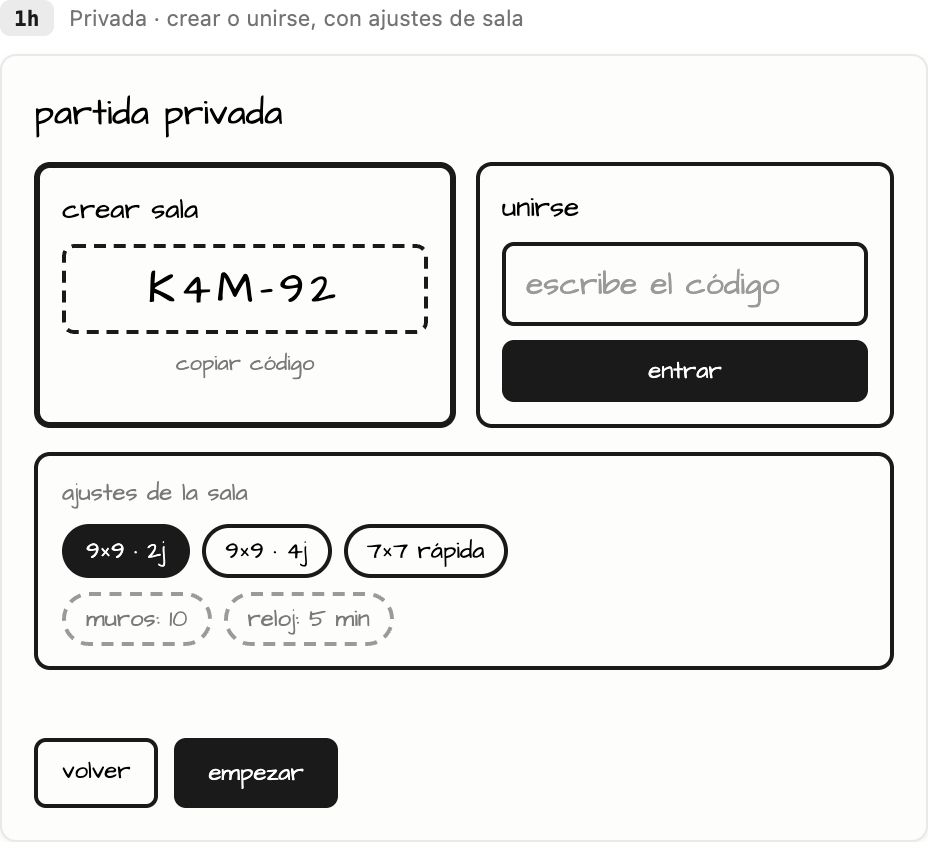
\includegraphics[width=\linewidth]{Prototipos/1h}\par\smallskip
{\footnotesize\textit{Prototipo 1h: Privada · crear o unirse, con ajustes de sala}}
\end{minipage}\hfill
\begin{minipage}[t]{0.48\textwidth}\centering
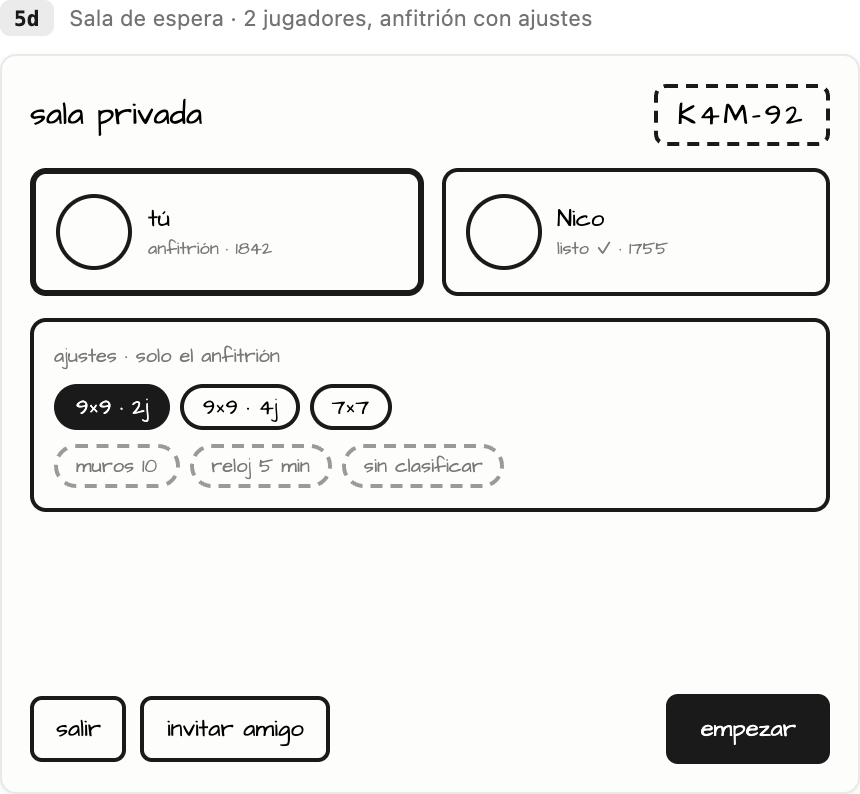
\includegraphics[width=\linewidth]{Prototipos/5d}\par\smallskip
{\footnotesize\textit{Prototipo 5d: Sala de espera · 2 jugadores}}
\end{minipage}
\par\medskip
\end{center}

%--- F-20 Unirse a una sala con código
\begin{prototipocrud}{F-20}{Unirse a una sala con código}
  \crudFila{Operación}{Creación (C), Actualización (U), Eliminación (D)}
  \crudFila{Caso de uso}{\mbox{CU-19}}
  \crudFila{Actor}{Jugador o invitado}
  \crudFila{Prototipos}{5e, Sala de espera · 4 plazas y chat de sala.}
  \crudFila{Datos de entrada}{\begin{crudlista}
    \item \texttt{codigo}: seis caracteres.
    \item Marca de listo.
    \item Token de sesión.
  \end{crudlista}}
  \crudFila{Datos que se consultan}{\begin{crudlista}
    \item \textit{Participacion}, \textit{ColaEmparejamiento}, \textit{SalaParticipante} y \textit{Sancion}: las mismas exclusiones que al crear una sala.
    \item \textit{Sala}: por \texttt{codigo} y \texttt{estado} = \texttt{ABIERTA}.
    \item \textit{Bloqueo}: entre el jugador y los miembros.
    \item \textit{Modo}: plazas.
    \item \textit{Mensaje}: los recientes del chat de sala.
  \end{crudlista}}
  \crudFila{Datos que se crean}{\begin{crudlista}
    \item \textit{SalaParticipante}: \texttt{id\_\allowbreak{}sala}, \texttt{id\_\allowbreak{}usuario}, \texttt{plaza}, \texttt{listo} = 0, \texttt{fecha\_\allowbreak{}union}.
  \end{crudlista}}
  \crudFila{Datos que se modifican}{\begin{crudlista}
    \item \textit{SalaParticipante}: \texttt{listo}.
  \end{crudlista}}
  \crudFila{Datos que se eliminan}{\begin{crudlista}
    \item \textit{SalaParticipante}: al salir de la sala, o si el jugador no reconecta en sesenta segundos. Borrado físico.
  \end{crudlista}}
  \crudFila{Reglas de negocio}{\begin{crudlista}
    \item Solo se entra a salas \texttt{ABIERTA} (\mbox{CU-19} \mbox{RN-01}).
    \item La última plaza se ocupa dentro de una transacción que vuelve a contar las libres (\mbox{CU-19} \mbox{RN-02}).
    \item Nadie está listo hasta que lo declara (\mbox{CU-19} \mbox{RN-03}).
    \item Los códigos fallidos por jugador están acotados (\mbox{CU-19} \mbox{RN-04}).
    \item Un bloqueo impide compartir sala y responde como un código inexistente (\mbox{CU-19} \mbox{RN-05}).
  \end{crudlista}}
  \crudFila{Resultado esperado}{El jugador ocupa una plaza en la sala, ve los ajustes y queda listo para que el anfitrión inicie.}
\end{prototipocrud}
\par\nopagebreak\smallskip
\begin{center}
\begin{minipage}[t]{0.50\textwidth}\centering
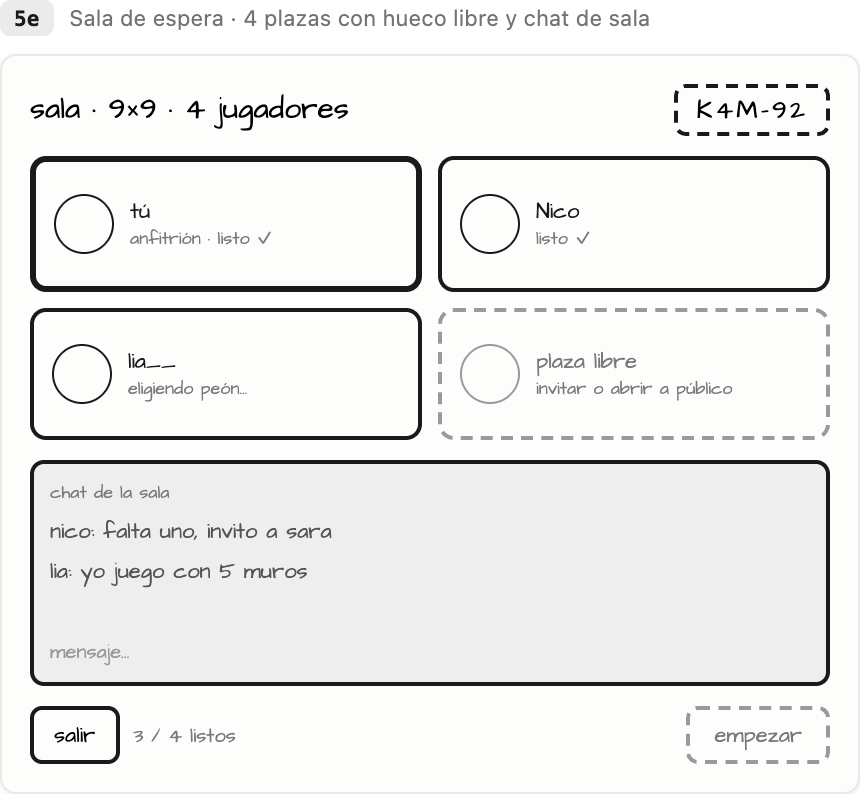
\includegraphics[width=\linewidth]{Prototipos/5e}\par\smallskip
{\footnotesize\textit{Prototipo 5e: Sala de espera · 4 plazas y chat de sala}}
\end{minipage}
\par\medskip
\end{center}

%--- F-21 Invitar a un jugador a una partida
\begin{prototipocrud}{F-21}{Invitar a un jugador a una partida}
  \crudFila{Operación}{Creación (C), Actualización (U)}
  \crudFila{Caso de uso}{\mbox{CU-32}}
  \crudFila{Actor}{Jugador}
  \crudFila{Prototipos}{2b, el botón ``invitar'' (\mbox{F-41}), y 10a, la opción ``retar'' (\mbox{F-39}).}
  \crudFila{Datos de entrada}{\begin{crudlista}
    \item \texttt{id\_\allowbreak{}usuario} del invitado.
    \item Ajustes de la sala, si no existe.
    \item Respuesta del invitado: aceptar o rechazar.
    \item Token de sesión.
  \end{crudlista}}
  \crudFila{Datos que se consultan}{\begin{crudlista}
    \item \textit{Participacion} y \textit{ColaEmparejamiento}: del emisor y del invitado.
    \item \textit{Bloqueo} y \textit{Usuario}: disponibilidad del invitado.
    \item \textit{Sesion}: que el invitado esté conectado.
    \item \textit{Invitacion}: pendientes del mismo emisor al mismo invitado.
  \end{crudlista}}
  \crudFila{Datos que se crean}{\begin{crudlista}
    \item \textit{Sala} y \textit{SalaParticipante} del emisor, si no estaba en una.
    \item \textit{Invitacion}: \texttt{id\_\allowbreak{}sala}, \texttt{id\_\allowbreak{}emisor}, \texttt{id\_\allowbreak{}destinatario}, \texttt{fecha\_\allowbreak{}invitacion}, \texttt{fecha\_\allowbreak{}expiracion}, \texttt{estado} = \texttt{PENDIENTE}.
    \item \textit{SalaParticipante} del invitado, al aceptar.
  \end{crudlista}}
  \crudFila{Datos que se modifican}{\begin{crudlista}
    \item \textit{Invitacion}: \texttt{estado} = \texttt{ACEPTADA}, \texttt{RECHAZADA} o \texttt{EXPIRADA}.
  \end{crudlista}}
  \crudFila{Datos que se eliminan}{Ninguno.}
  \crudFila{Reglas de negocio}{\begin{crudlista}
    \item Se puede retar a cualquier jugador, sea o no amigo, si no hay bloqueo (\mbox{CU-32} \mbox{RN-02}, \mbox{RN-03}).
    \item Una invitación expira a los sesenta segundos y no se duplica (\mbox{CU-32} \mbox{RN-04}).
    \item Aceptar da acceso a la sala sin conocer su código (\mbox{CU-32} \mbox{RN-05}).
    \item Solo se invita a jugadores conectados que no estén en una partida en línea (\mbox{CU-32} \mbox{RN-06}).
  \end{crudlista}}
  \crudFila{Resultado esperado}{Emisor e invitado están en la misma sala privada, o la invitación quedó rechazada o expirada.}
\end{prototipocrud}

\subsection*{Partida}
\addcontentsline{toc}{subsection}{Partida}

La partida concentra el mayor volumen de escrituras del sistema. Se registra jugada por jugada porque de ello dependen la repetición, la reconexión y las pruebas de los reportes, y se cierra en una sola operación que aplica todas sus consecuencias a la vez.

%--- F-22 Registrar jugada
\begin{prototipocrud}{F-22}{Registrar jugada}
  \crudFila{Operación}{Creación (C)}
  \crudFila{Caso de uso}{\mbox{CU-20}, \mbox{CU-21}}
  \crudFila{Actor}{Jugador}
  \crudFila{Prototipos}{20a, Partida · peón seleccionado; 21a, Partida · muro cogido con cartel flotante.}
  \crudFila{Datos de entrada}{\begin{crudlista}
    \item \texttt{tipo}: \texttt{MOVIMIENTO} o \texttt{MURO}.
    \item Para un movimiento: \texttt{casilla\_\allowbreak{}destino}.
    \item Para un muro: \texttt{surco} y \texttt{orientacion} (horizontal o vertical).
    \item \texttt{numero\_\allowbreak{}jugada} esperado.
    \item Token de sesión.
  \end{crudlista}}
  \crudFila{Datos que se consultan}{\begin{crudlista}
    \item \textit{Partida}: \texttt{estado}, \texttt{turno\_\allowbreak{}actual}.
    \item \textit{Participacion} de todos los jugadores: \texttt{casilla\_\allowbreak{}actual}, \texttt{muros\_\allowbreak{}restantes}, \texttt{reloj\_\allowbreak{}restante}, \texttt{posicion}.
    \item \textit{Jugada}: todas las de la partida, para reconstruir el tablero.
  \end{crudlista}}
  \crudFila{Datos que se crean}{\begin{crudlista}
    \item \textit{Jugada}: \texttt{id\_\allowbreak{}partida}, \texttt{numero\_\allowbreak{}jugada}, \texttt{id\_\allowbreak{}usuario}, \texttt{tipo}, \texttt{casilla\_\allowbreak{}origen}, \texttt{casilla\_\allowbreak{}destino}, \texttt{surco}, \texttt{orientacion}, \texttt{tiempo\_\allowbreak{}consumido}, \texttt{fecha\_\allowbreak{}jugada}, \texttt{deshecha} = 0.
  \end{crudlista}}
  \crudFila{Datos que se modifican}{\begin{crudlista}
    \item \textit{Participacion}: \texttt{casilla\_\allowbreak{}actual} o \texttt{muros\_\allowbreak{}restantes}, \texttt{reloj\_\allowbreak{}restante} y, si llega a meta, \texttt{posicion}.
    \item \textit{Partida}: \texttt{turno\_\allowbreak{}actual}.
    \item \textit{OfertaTablas} pendiente del rival: \texttt{estado} = \texttt{CADUCADA} (\mbox{CU-22} \mbox{RN-05}).
  \end{crudlista}}
  \crudFila{Datos que se eliminan}{Ninguna. Las jugadas no se borran y los muros no se retiran.}
  \crudFila{Reglas de negocio}{\begin{crudlista}
    \item El servidor es la única autoridad sobre el estado del tablero (\mbox{CU-20} \mbox{RN-01}).
    \item El peón se mueve una casilla en ortogonal o salta al rival adyacente (\mbox{CU-20} \mbox{RN-02}, \mbox{RN-03}).
    \item El muro mide dos casillas, no se solapa ni se cruza y nunca deja a un jugador sin camino (\mbox{CU-21} \mbox{RN-03}, \mbox{RN-04}, \mbox{RN-05}).
    \item Las jugadas llevan número consecutivo; una fuera de orden se rechaza (\mbox{CU-20} \mbox{RN-06}).
    \item En cada turno se hace exactamente una acción (\mbox{CU-20} \mbox{RN-05}).
    \item Jugada, participación y turno se escriben en una transacción (\mbox{CU-20} \mbox{RN-12}).
  \end{crudlista}}
  \crudFila{Resultado esperado}{La jugada queda registrada, el tablero y el reloj reflejan su efecto y el turno pasa al siguiente jugador activo.}
\end{prototipocrud}
\par\nopagebreak\smallskip
\begin{center}
\begin{minipage}[t]{0.48\textwidth}\centering
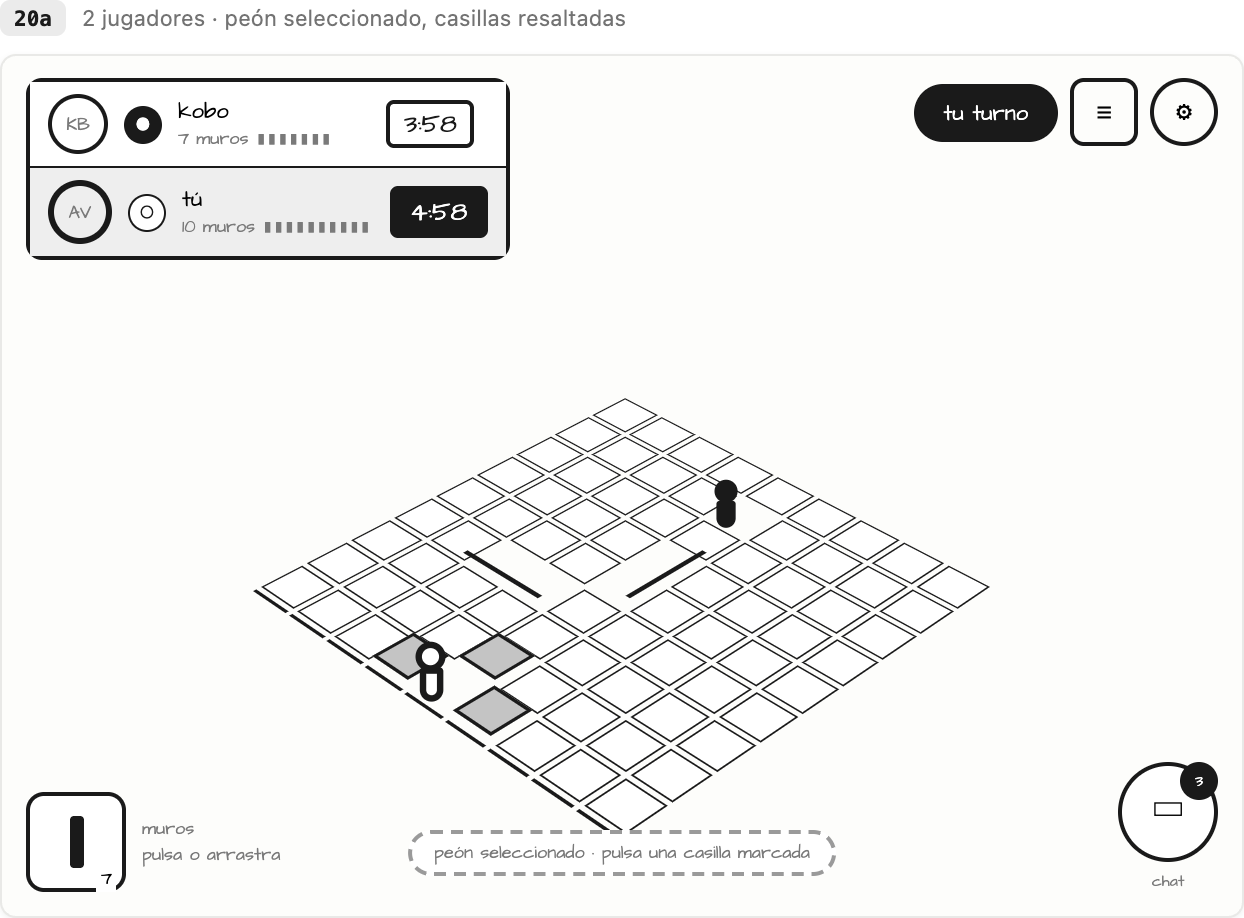
\includegraphics[width=\linewidth]{Prototipos/20a}\par\smallskip
{\footnotesize\textit{Prototipo 20a: Partida · peón seleccionado}}
\end{minipage}\hfill
\begin{minipage}[t]{0.48\textwidth}\centering
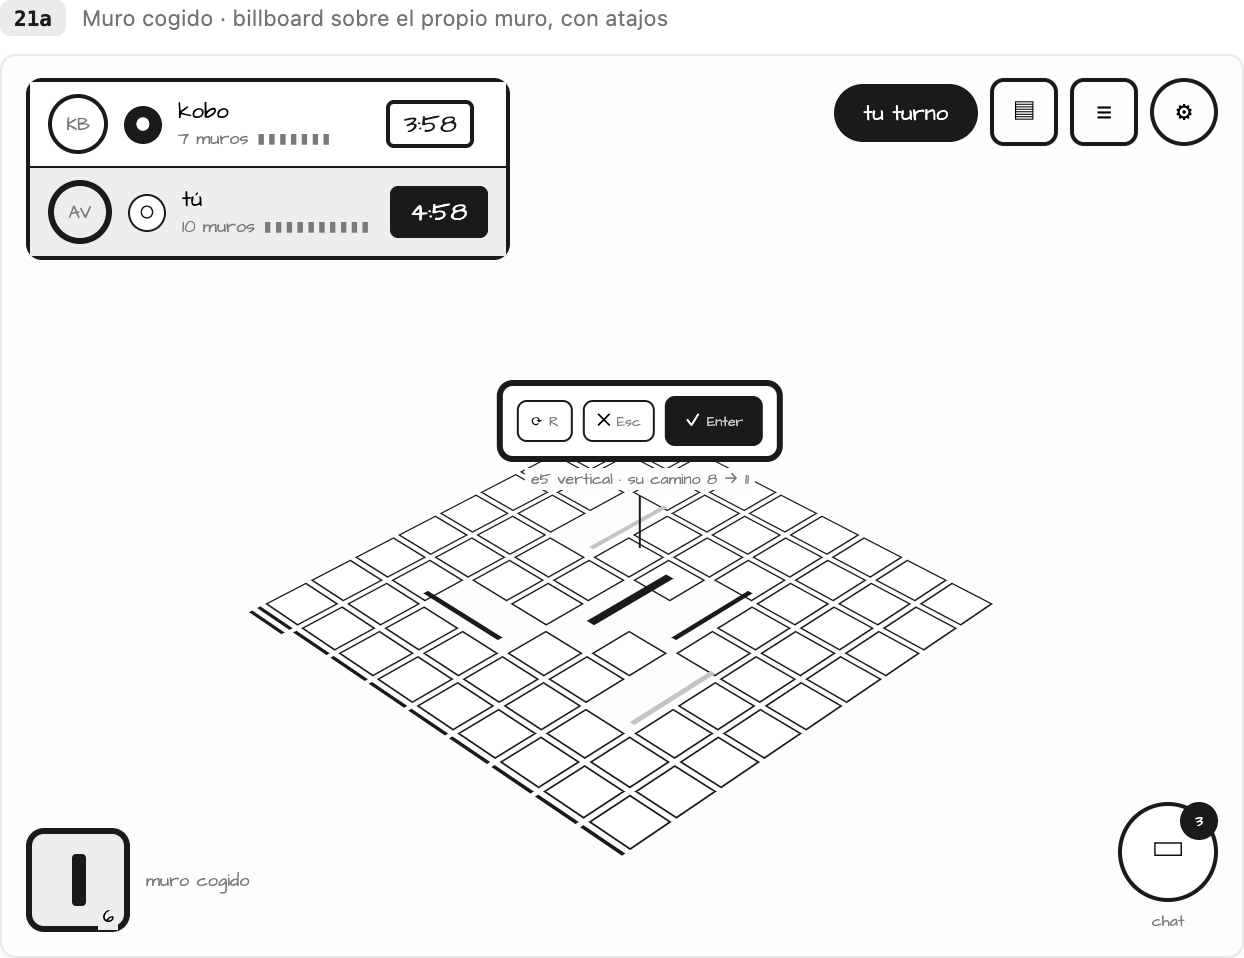
\includegraphics[width=\linewidth]{Prototipos/21a}\par\smallskip
{\footnotesize\textit{Prototipo 21a: Partida · muro cogido con cartel flotante}}
\end{minipage}
\par\medskip
\end{center}

%--- F-23 Ofrecer y responder tablas
\begin{prototipocrud}{F-23}{Ofrecer y responder tablas}
  \crudFila{Operación}{Creación (C), Actualización (U)}
  \crudFila{Caso de uso}{\mbox{CU-22}}
  \crudFila{Actor}{Jugador, y su rival al responder}
  \crudFila{Prototipos}{19d, Menú de partida · rendirse y tablas.}
  \crudFila{Datos de entrada}{\begin{crudlista}
    \item Oferta: token de sesión.
    \item Respuesta: aceptar o rechazar.
  \end{crudlista}}
  \crudFila{Datos que se consultan}{\begin{crudlista}
    \item \textit{Partida} y \textit{Modo}: \texttt{estado}, \texttt{tipo} y número de jugadores.
    \item \textit{OfertaTablas}: pendientes de la partida y ofertas recientes del jugador.
  \end{crudlista}}
  \crudFila{Datos que se crean}{\begin{crudlista}
    \item \textit{OfertaTablas}: \texttt{id\_\allowbreak{}partida}, \texttt{id\_\allowbreak{}ofertante}, \texttt{numero\_\allowbreak{}jugada}, \texttt{fecha\_\allowbreak{}oferta}, \texttt{estado} = \texttt{PENDIENTE}.
  \end{crudlista}}
  \crudFila{Datos que se modifican}{\begin{crudlista}
    \item \textit{OfertaTablas}: \texttt{estado} = \texttt{ACEPTADA}, \texttt{RECHAZADA} o \texttt{CADUCADA}, y \texttt{fecha\_\allowbreak{}respuesta}.
  \end{crudlista}}
  \crudFila{Datos que se eliminan}{Ninguno.}
  \crudFila{Reglas de negocio}{\begin{crudlista}
    \item Solo en partidas de dos jugadores y no contra la IA (\mbox{CU-22} \mbox{RN-01}, \mbox{D-14}).
    \item Ofrecer no detiene la partida ni el reloj (\mbox{CU-22} \mbox{RN-02}).
    \item Una oferta cada cinco jugadas propias como máximo (\mbox{CU-22} \mbox{RN-03}).
    \item Dos ofertas cruzadas son un acuerdo (\mbox{CU-22} \mbox{RN-04}).
    \item La oferta caduca en cuanto el rival juega (\mbox{CU-22} \mbox{RN-05}).
  \end{crudlista}}
  \crudFila{Resultado esperado}{Si se acepta, la partida continúa en su cierre con \texttt{forma\_\allowbreak{}termino} = \texttt{TABLAS}; si no, la oferta queda rechazada o caducada y la partida sigue.}
\end{prototipocrud}
\par\nopagebreak\smallskip
\begin{center}
\begin{minipage}[t]{0.50\textwidth}\centering
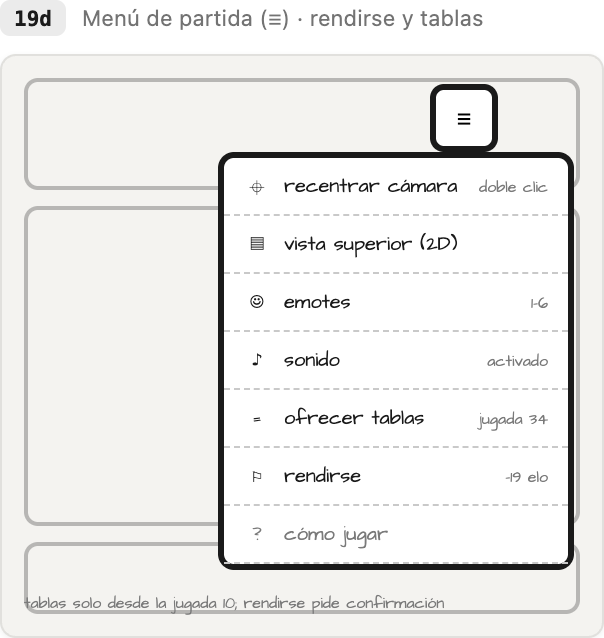
\includegraphics[width=\linewidth]{Prototipos/19d}\par\smallskip
{\footnotesize\textit{Prototipo 19d: Menú de partida · rendirse y tablas}}
\end{minipage}
\par\medskip
\end{center}

%--- F-24 Rendirse
\begin{prototipocrud}{F-24}{Rendirse}
  \crudFila{Operación}{Actualización (U)}
  \crudFila{Caso de uso}{\mbox{CU-23}}
  \crudFila{Actor}{Jugador}
  \crudFila{Prototipos}{19d, la opción ``rendirse'' (\mbox{F-23}).}
  \crudFila{Datos de entrada}{\begin{crudlista}
    \item Confirmación tras ver el elo que se perdería.
    \item Token de sesión.
  \end{crudlista}}
  \crudFila{Datos que se consultan}{\begin{crudlista}
    \item \textit{Participacion}: \texttt{elo\_\allowbreak{}inicial} del jugador y de sus rivales, para la vista previa.
    \item \textit{Partida} y \textit{Modo}: \texttt{estado}, \texttt{tipo} y número de jugadores.
  \end{crudlista}}
  \crudFila{Datos que se crean}{Ninguno.}
  \crudFila{Datos que se modifican}{\begin{crudlista}
    \item \textit{OfertaTablas} pendiente: \texttt{estado} = \texttt{CADUCADA}.
    \item En cuatro jugadores: la \textit{Participacion} del jugador recibe \texttt{resultado}, \texttt{posicion}, \texttt{forma\_\allowbreak{}termino} = \texttt{RENDICION} y \texttt{terminada} = 1.
    \item En dos jugadores: el cierre de la partida con \texttt{forma\_\allowbreak{}termino} = \texttt{RENDICION}.
  \end{crudlista}}
  \crudFila{Datos que se eliminan}{Ninguno.}
  \crudFila{Reglas de negocio}{\begin{crudlista}
    \item Se puede rendir en cualquier momento, sea o no su turno (\mbox{CU-23} \mbox{RN-01}).
    \item La confirmación muestra el elo que se perderá, calculado igual que en el cierre (\mbox{CU-23} \mbox{RN-02}).
    \item En cuatro jugadores retira al jugador; sus muros se quedan (\mbox{CU-23} \mbox{RN-04}).
    \item Cuenta como derrota y rompe la racha (\mbox{CU-23} \mbox{RN-05}).
  \end{crudlista}}
  \crudFila{Resultado esperado}{El jugador pierde la partida; en cuatro jugadores la partida sigue para los demás.}
\end{prototipocrud}

%--- F-25 Abandonar la partida o reclamar la victoria
\begin{prototipocrud}{F-25}{Abandonar la partida o reclamar la victoria}
  \crudFila{Operación}{Actualización (U)}
  \crudFila{Caso de uso}{\mbox{CU-24}}
  \crudFila{Actor}{Jugador, o el rival de un jugador desconectado}
  \crudFila{Prototipos}{8e, 4 jugadores · eliminado y abandono; 6f, Rival desconectado · esperando.}
  \crudFila{Datos de entrada}{\begin{crudlista}
    \item Abandonar: la palabra de confirmación escrita.
    \item Reclamar la victoria: la orden, tras sesenta segundos de desconexión del rival.
    \item Token de sesión.
  \end{crudlista}}
  \crudFila{Datos que se consultan}{\begin{crudlista}
    \item \textit{Participacion}: la propia y, al reclamar, \texttt{conectado} y \texttt{fecha\_\allowbreak{}desconexion} del rival.
    \item \textit{Partida} y \textit{Modo}: \texttt{estado}, \texttt{tipo} y número de jugadores.
  \end{crudlista}}
  \crudFila{Datos que se crean}{Ninguno.}
  \crudFila{Datos que se modifican}{\begin{crudlista}
    \item \textit{EstadisticaModo} del que abandona: \texttt{abandonos}, en partidas en línea.
    \item \textit{OfertaTablas} pendiente: \texttt{estado} = \texttt{CADUCADA}.
    \item \textit{Participacion} del que abandona en cuatro jugadores: \texttt{resultado}, \texttt{posicion}, \texttt{forma\_\allowbreak{}termino} = \texttt{ABANDONO}, \texttt{terminada} = 1.
    \item En dos jugadores: el cierre de la partida con \texttt{forma\_\allowbreak{}termino} = \texttt{ABANDONO}.
  \end{crudlista}}
  \crudFila{Datos que se eliminan}{Ninguno.}
  \crudFila{Reglas de negocio}{\begin{crudlista}
    \item Abandonar cuenta como derrota a todos los efectos (\mbox{CU-24} \mbox{RN-01}, \mbox{D-15}).
    \item Exige escribir la palabra de confirmación (\mbox{CU-24} \mbox{RN-02}).
    \item Cerrar el juego o perder la conexión no es abandonar (\mbox{CU-24} \mbox{RN-03}).
    \item El rival puede reclamar la victoria a los sesenta segundos de desconexión (\mbox{CU-24} \mbox{RN-06}).
    \item Los abandonos se cuentan por modo para la moderación (\mbox{CU-24} \mbox{RN-05}).
  \end{crudlista}}
  \crudFila{Resultado esperado}{El que abandona pierde la partida, su contador de abandonos aumenta y su peón sale del tablero; sus muros permanecen.}
\end{prototipocrud}
\par\nopagebreak\smallskip
\begin{center}
\begin{minipage}[t]{0.48\textwidth}\centering
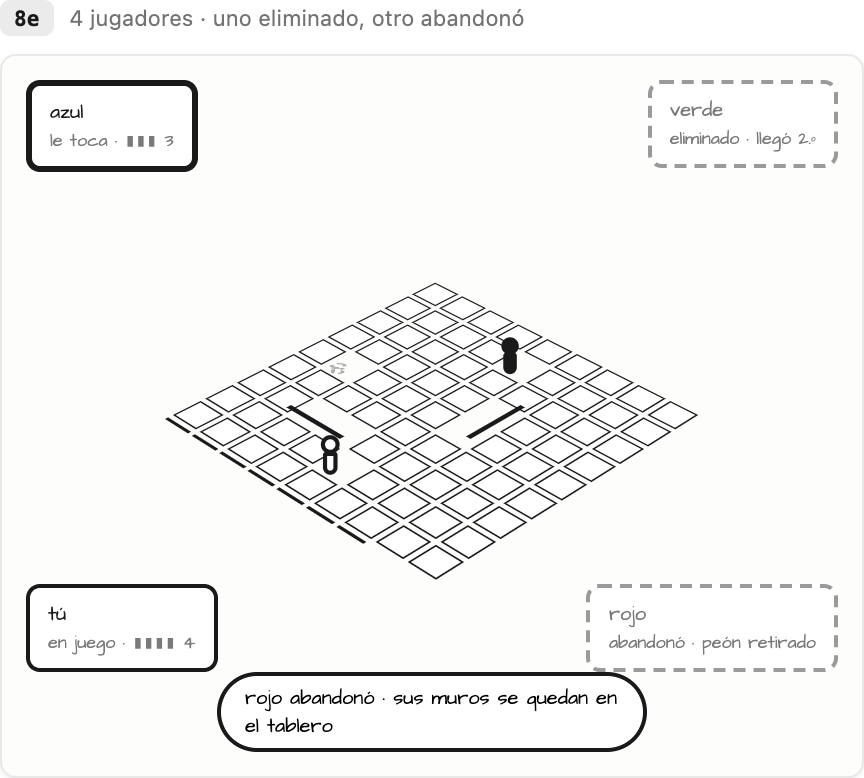
\includegraphics[width=\linewidth]{Prototipos/8e}\par\smallskip
{\footnotesize\textit{Prototipo 8e: 4 jugadores · eliminado y abandono}}
\end{minipage}\hfill
\begin{minipage}[t]{0.48\textwidth}\centering
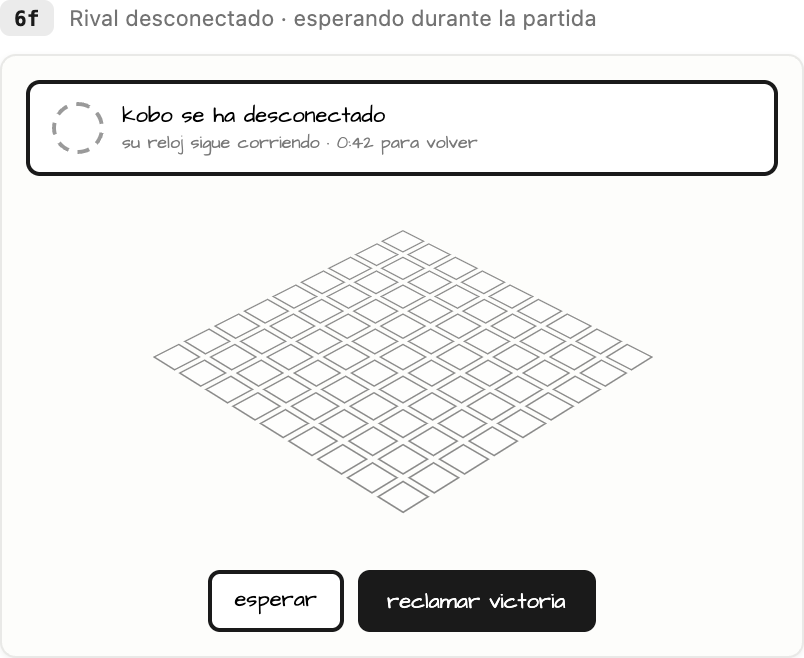
\includegraphics[width=\linewidth]{Prototipos/6f}\par\smallskip
{\footnotesize\textit{Prototipo 6f: Rival desconectado · esperando}}
\end{minipage}
\par\medskip
\end{center}

%--- F-26 Reconectar a una partida en curso
\begin{prototipocrud}{F-26}{Reconectar a una partida en curso}
  \crudFila{Operación}{Actualización (U)}
  \crudFila{Caso de uso}{\mbox{CU-26}}
  \crudFila{Actor}{Jugador}
  \crudFila{Prototipos}{6e, Reconexión · la partida sigue viva.}
  \crudFila{Datos de entrada}{\begin{crudlista}
    \item Token de sesión, desde el mismo u otro dispositivo.
  \end{crudlista}}
  \crudFila{Datos que se consultan}{\begin{crudlista}
    \item \textit{Participacion} sin terminar del jugador y las de todos los participantes.
    \item \textit{Partida}: \texttt{estado}, \texttt{turno\_\allowbreak{}actual}.
    \item \textit{Jugada}: todas en orden.
    \item \textit{ParticipacionObjeto} y \textit{OfertaTablas} pendiente.
  \end{crudlista}}
  \crudFila{Datos que se crean}{Ninguno.}
  \crudFila{Datos que se modifican}{\begin{crudlista}
    \item \textit{Participacion}: \texttt{conectado} = 0 y \texttt{fecha\_\allowbreak{}desconexion} al perder la conexión; \texttt{conectado} = 1 al volver.
  \end{crudlista}}
  \crudFila{Datos que se eliminan}{Ninguno.}
  \crudFila{Reglas de negocio}{\begin{crudlista}
    \item La desconexión no detiene el reloj (\mbox{CU-26} \mbox{RN-01}).
    \item Una partida admite una conexión por participante: reconectar desde otro dispositivo toma el control sin cerrar la otra sesión (\mbox{CU-26} \mbox{RN-04}).
    \item Si el que se cae es el servidor, ese tiempo no se descuenta de ningún reloj (\mbox{CU-26} \mbox{RN-05}).
    \item El cliente nunca reconstruye el tablero con un estado parcial (\mbox{CU-26} \mbox{RN-06}).
  \end{crudlista}}
  \crudFila{Resultado esperado}{El jugador vuelve a la partida en el mismo estado que tiene el servidor, o ve el resultado si terminó mientras estaba fuera.}
\end{prototipocrud}
\par\nopagebreak\smallskip
\begin{center}
\begin{minipage}[t]{0.50\textwidth}\centering
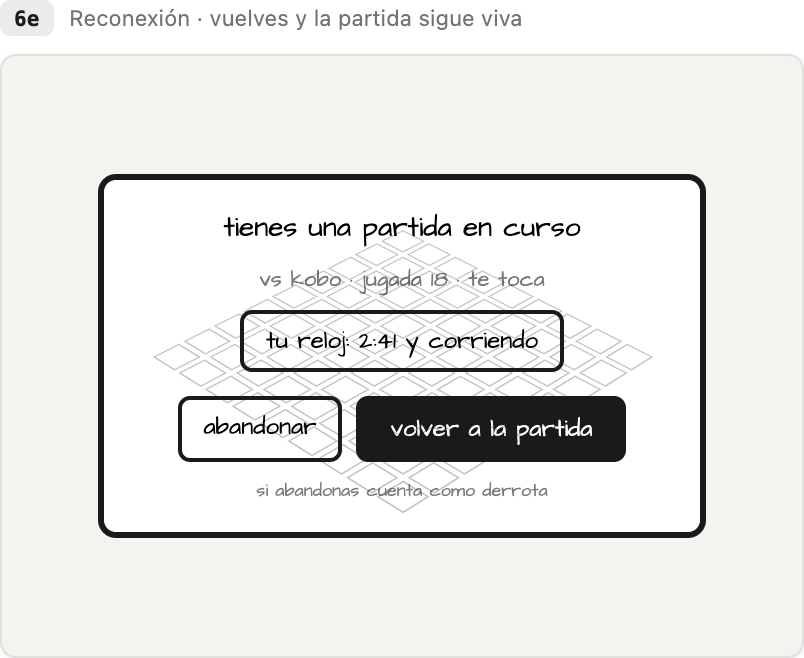
\includegraphics[width=\linewidth]{Prototipos/6e}\par\smallskip
{\footnotesize\textit{Prototipo 6e: Reconexión · la partida sigue viva}}
\end{minipage}
\par\medskip
\end{center}

%--- F-27 Jugar contra la IA
\begin{prototipocrud}{F-27}{Jugar contra la IA}
  \crudFila{Operación}{Creación (C), Actualización (U)}
  \crudFila{Caso de uso}{\mbox{CU-27}}
  \crudFila{Actor}{Jugador o invitado}
  \crudFila{Prototipos}{8f, Contra la IA · elegir dificultad; 12f, Contra la IA · deshacer y sugerencia.}
  \crudFila{Datos de entrada}{\begin{crudlista}
    \item \texttt{id\_\allowbreak{}nivel\_\allowbreak{}ia}: aprendiz, constructor, arquitecto o bastión.
    \item \texttt{id\_\allowbreak{}modo}: 9×9 o 7×7.
    \item \texttt{minutos\_\allowbreak{}reloj}, o sin reloj.
    \item \texttt{permite\_\allowbreak{}deshacer} y \texttt{permite\_\allowbreak{}sugerencias}.
    \item Durante la partida: órdenes de deshacer y de sugerencia.
    \item Token de sesión.
  \end{crudlista}}
  \crudFila{Datos que se consultan}{\begin{crudlista}
    \item \textit{NivelIA} y \textit{Modo}.
    \item \textit{ColaEmparejamiento}, \textit{SalaParticipante} y \textit{Participacion}: exclusiones.
    \item \textit{Jugada}: para calcular la jugada de la IA, las sugerencias y el repaso.
  \end{crudlista}}
  \crudFila{Datos que se crean}{\begin{crudlista}
    \item \textit{Partida}: \texttt{tipo} = \texttt{IA}, \texttt{id\_\allowbreak{}nivel\_\allowbreak{}ia}, \texttt{id\_\allowbreak{}modo}, \texttt{minutos\_\allowbreak{}reloj}, \texttt{permite\_\allowbreak{}deshacer}, \texttt{permite\_\allowbreak{}sugerencias}, \texttt{estado} = \texttt{EN\_\allowbreak{}CURSO}, \texttt{fecha\_\allowbreak{}inicio}.
    \item \textit{Participacion} y \textit{ParticipacionObjeto} del jugador; la IA no tiene participación.
    \item \textit{Jugada} de la IA, con \texttt{id\_\allowbreak{}usuario} nulo.
  \end{crudlista}}
  \crudFila{Datos que se modifican}{\begin{crudlista}
    \item \textit{Partida}: \texttt{deshacer\_\allowbreak{}usados}, \texttt{sugerencias\_\allowbreak{}usadas}; se cierra con \texttt{ABANDONO} la partida contra la IA anterior sin terminar.
    \item \textit{Jugada}: \texttt{deshecha} = 1 al deshacer.
    \item \textit{Participacion}: se restablece al estado anterior al deshacer.
  \end{crudlista}}
  \crudFila{Datos que se eliminan}{Ninguno.}
  \crudFila{Reglas de negocio}{\begin{crudlista}
    \item No otorga elo ni monedas, sí experiencia (\mbox{CU-27} \mbox{RN-01}).
    \item La IA no es un \textit{Usuario} y sus jugadas se validan con las mismas reglas (\mbox{CU-27} \mbox{RN-03}, \mbox{RN-04}).
    \item Deshacer marca las jugadas, no las borra (\mbox{CU-27} \mbox{RN-05}).
    \item Una partida contra la IA pendiente se cierra sola al entrar a otra partida (\mbox{CU-27} \mbox{RN-07}, \mbox{D-11}).
    \item Se guarda en el servidor para el historial, la repetición y el repaso (\mbox{D-12}).
  \end{crudlista}}
  \crudFila{Resultado esperado}{Existe una partida contra la IA registrada con sus jugadas; al terminar, el jugador recibe experiencia y un repaso de tres errores.}
\end{prototipocrud}
\par\nopagebreak\smallskip
\begin{center}
\begin{minipage}[t]{0.48\textwidth}\centering
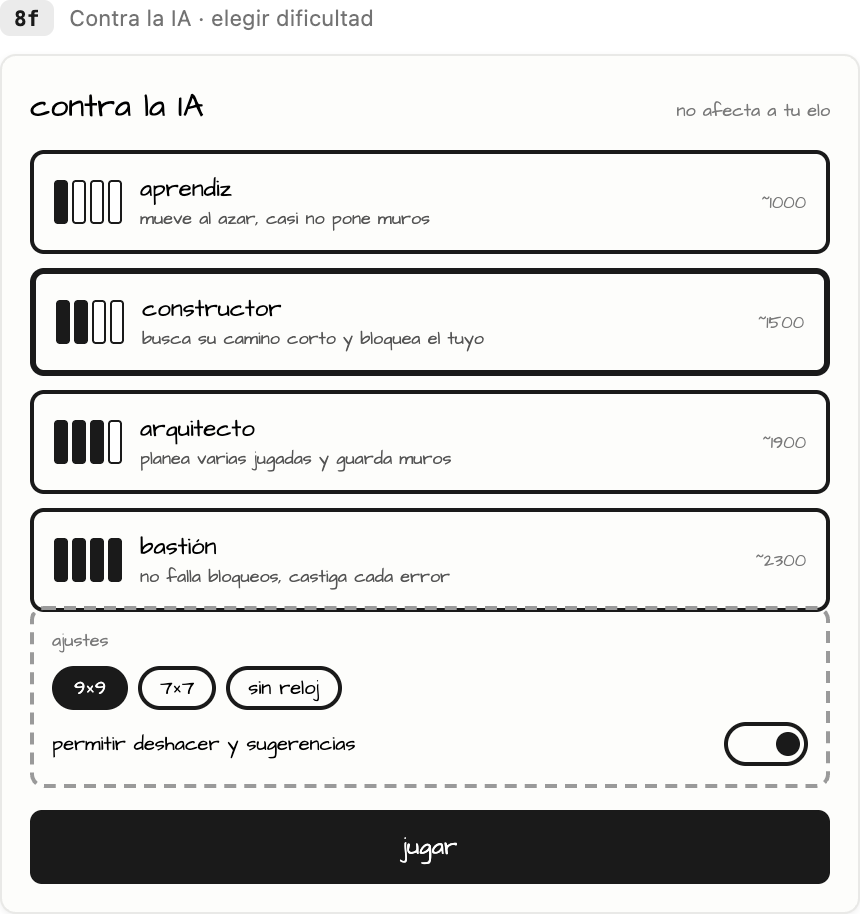
\includegraphics[width=\linewidth]{Prototipos/8f}\par\smallskip
{\footnotesize\textit{Prototipo 8f: Contra la IA · elegir dificultad}}
\end{minipage}\hfill
\begin{minipage}[t]{0.48\textwidth}\centering
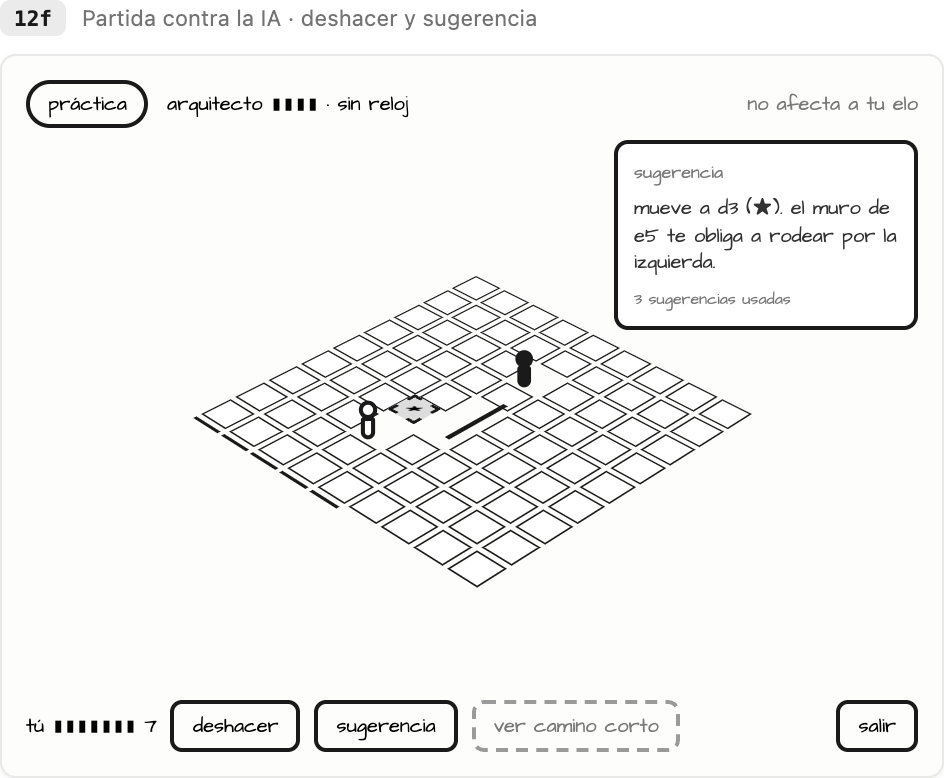
\includegraphics[width=\linewidth]{Prototipos/12f}\par\smallskip
{\footnotesize\textit{Prototipo 12f: Contra la IA · deshacer y sugerencia}}
\end{minipage}
\par\medskip
\end{center}

%--- F-28 Finalizar partida
\begin{prototipocrud}{F-28}{Finalizar partida}
  \crudFila{Operación}{Actualización (U), Creación (C)}
  \crudFila{Caso de uso}{\mbox{CU-25}}
  \crudFila{Actor}{Servidor de partidas}
  \crudFila{Prototipos}{2g, Fin de partida · tarjeta sobre el tablero; 11a, Subida de nivel; 11b, Subida de división.}
  \crudFila{Datos de entrada}{\begin{crudlista}
    \item \texttt{id\_\allowbreak{}partida}.
    \item \texttt{forma\_\allowbreak{}termino}: \texttt{META}, \texttt{TIEMPO\_\allowbreak{}AGOTADO}, \texttt{RENDICION}, \texttt{TABLAS} o \texttt{ABANDONO}.
    \item Jugador que provocó el término, si aplica.
  \end{crudlista}}
  \crudFila{Datos que se consultan}{\begin{crudlista}
    \item \textit{Partida}: \texttt{tipo}, \texttt{id\_\allowbreak{}modo}.
    \item \textit{Participacion}: \texttt{elo\_\allowbreak{}inicial} de cada jugador.
    \item \textit{Jugada}: las de tipo \texttt{MURO} de cada jugador y, contra la IA, todas para el repaso.
    \item \textit{Modo}, \textit{Division}, \textit{EstadisticaModo} y \textit{Usuario}: \texttt{nivel}, \texttt{experiencia}.
  \end{crudlista}}
  \crudFila{Datos que se crean}{\begin{crudlista}
    \item \textit{MovimientoMoneda}: \texttt{tipo} = \texttt{PARTIDA} por participante y, si sube de nivel, \texttt{NIVEL}.
    \item \textit{HistorialDivision}: por cada cambio de división.
    \item \textit{UsuarioObjeto} y \textit{Caja} con \texttt{origen} = \texttt{PARTIDA}: recompensas de nivel.
  \end{crudlista}}
  \crudFila{Datos que se modifican}{\begin{crudlista}
    \item \textit{Partida}: \texttt{estado} = \texttt{FINALIZADA}, \texttt{fecha\_\allowbreak{}fin}, \texttt{forma\_\allowbreak{}termino}, \texttt{id\_\allowbreak{}ganador}.
    \item \textit{Participacion}: \texttt{resultado}, \texttt{posicion}, \texttt{elo\_\allowbreak{}final}, \texttt{diferencia\_\allowbreak{}elo}, \texttt{reloj\_\allowbreak{}restante}, \texttt{terminada} = 1.
    \item \textit{EstadisticaModo}: \texttt{partidas\_\allowbreak{}jugadas}, \texttt{partidas\_\allowbreak{}ganadas} o \texttt{partidas\_\allowbreak{}perdidas}, \texttt{puntos\_\allowbreak{}elo}, \texttt{elo\_\allowbreak{}maximo}, \texttt{racha\_\allowbreak{}actual}, \texttt{mejor\_\allowbreak{}racha}, \texttt{tiempo\_\allowbreak{}total\_\allowbreak{}jugado}, \texttt{barreras\_\allowbreak{}colocadas}, \texttt{division}.
    \item \textit{Usuario}: \texttt{experiencia}, \texttt{nivel}, \texttt{saldo\_\allowbreak{}monedas}.
    \item \textit{EnlaceEspectador}: \texttt{activo} = 0.
    \item \textit{Sala} de origen: \texttt{estado} = \texttt{CERRADA}.
  \end{crudlista}}
  \crudFila{Datos que se eliminan}{\begin{crudlista}
    \item \textit{SalaParticipante}: los miembros de la sala de origen.
  \end{crudlista}}
  \crudFila{Reglas de negocio}{\begin{crudlista}
    \item Solo las partidas clasificatorias otorgan elo y monedas (\mbox{CU-25} \mbox{RN-03}).
    \item El elo se calcula desde \texttt{elo\_\allowbreak{}inicial} (\mbox{CU-25} \mbox{RN-04}).
    \item Una victoria por reloj no cuenta para la racha limpia (\mbox{CU-25} \mbox{RN-11}).
    \item Los cambios de división respetan unas partidas de margen (\mbox{CU-25} \mbox{RN-07}).
    \item Todo el cierre ocurre en una sola transacción; si falla, la partida queda \texttt{PENDIENTE\_\allowbreak{}DE\_\allowbreak{}CIERRE} y se reintenta (\mbox{CU-25} \mbox{RN-12}, \mbox{RN-13}).
  \end{crudlista}}
  \crudFila{Resultado esperado}{La partida queda finalizada, cada jugador tiene su resultado y su cambio de elo, y las estadísticas, el nivel, la división y las monedas reflejan la partida.}
\end{prototipocrud}
\par\nopagebreak\smallskip
\begin{center}
\begin{minipage}[t]{0.48\textwidth}\centering
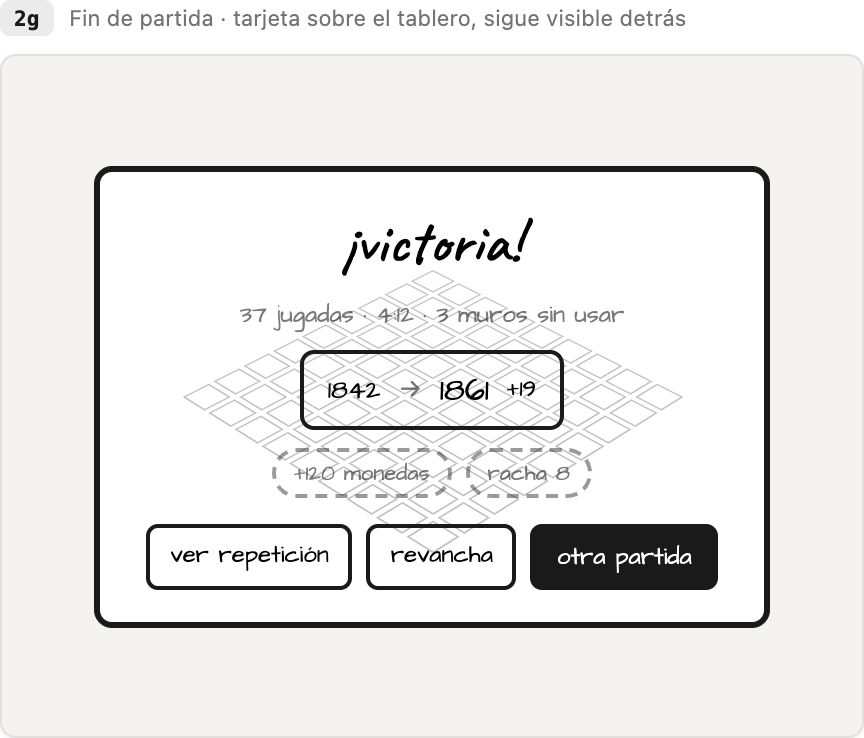
\includegraphics[width=\linewidth]{Prototipos/2g}\par\smallskip
{\footnotesize\textit{Prototipo 2g: Fin de partida · tarjeta sobre el tablero}}
\end{minipage}\hfill
\begin{minipage}[t]{0.48\textwidth}\centering
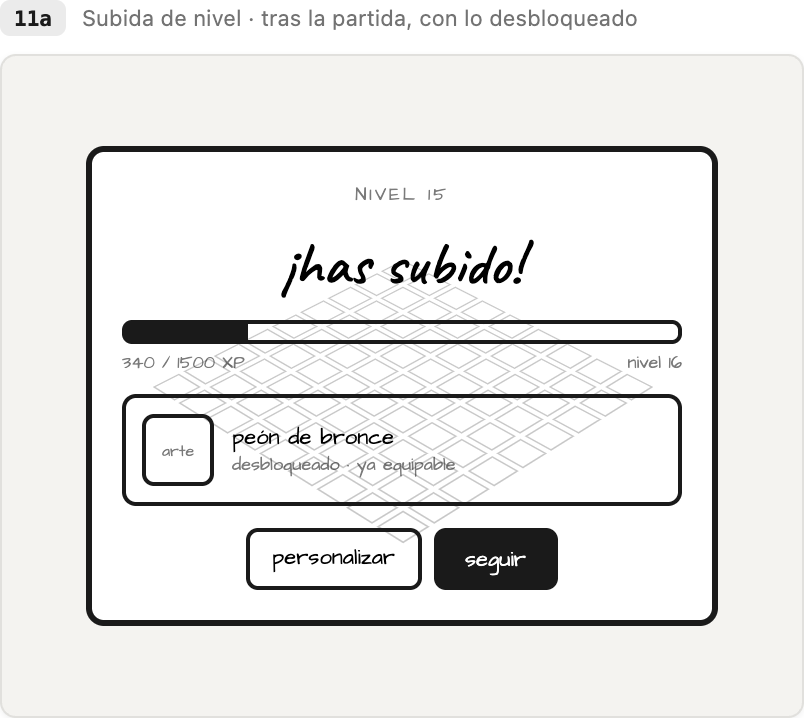
\includegraphics[width=\linewidth]{Prototipos/11a}\par\smallskip
{\footnotesize\textit{Prototipo 11a: Subida de nivel}}
\end{minipage}
\par\medskip
\begin{minipage}[t]{0.50\textwidth}\centering
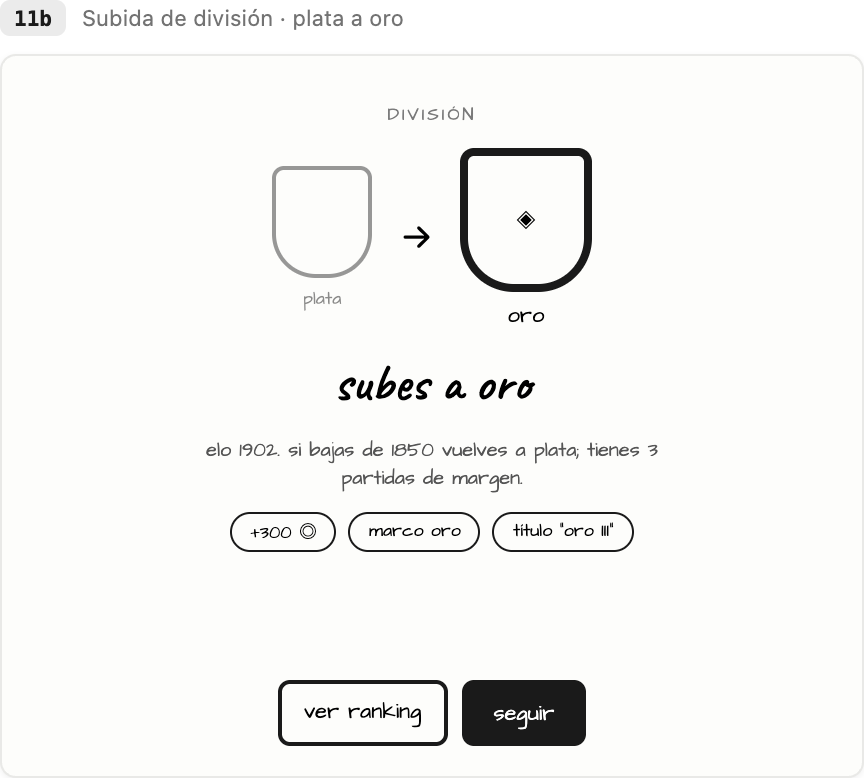
\includegraphics[width=\linewidth]{Prototipos/11b}\par\smallskip
{\footnotesize\textit{Prototipo 11b: Subida de división}}
\end{minipage}
\par\medskip
\end{center}

%--- F-29 Consultar historial de partidas
\begin{prototipocrud}{F-29}{Consultar historial de partidas}
  \crudFila{Operación}{Consulta (R)}
  \crudFila{Caso de uso}{\mbox{CU-36}}
  \crudFila{Actor}{Jugador o invitado}
  \crudFila{Prototipos}{17f, Historial · filtros por modo y final.}
  \crudFila{Datos de entrada}{\begin{crudlista}
    \item Filtros opcionales: \texttt{id\_\allowbreak{}modo} y \texttt{forma\_\allowbreak{}termino}.
    \item Página solicitada.
    \item Token de sesión.
  \end{crudlista}}
  \crudFila{Datos que se consultan}{\begin{crudlista}
    \item \textit{Participacion} del jugador: \texttt{resultado}, \texttt{posicion}, \texttt{diferencia\_\allowbreak{}elo}.
    \item \textit{Partida}: \texttt{id\_\allowbreak{}modo}, \texttt{tipo}, \texttt{estado}, \texttt{forma\_\allowbreak{}termino}, \texttt{fecha\_\allowbreak{}inicio}, \texttt{fecha\_\allowbreak{}fin}.
    \item \textit{Modo} y \textit{NivelIA}: nombres.
    \item \textit{Participacion} de los rivales y su \textit{Usuario}: \texttt{nickname}.
  \end{crudlista}}
  \crudFila{Datos que se crean}{Ninguno.}
  \crudFila{Datos que se modifican}{Ninguno.}
  \crudFila{Datos que se eliminan}{Ninguno.}
  \crudFila{Reglas de negocio}{\begin{crudlista}
    \item La duración se calcula; no se almacena (\mbox{CU-36} \mbox{RN-02}).
    \item El cambio de elo es el guardado en la participación (\mbox{CU-36} \mbox{RN-03}).
    \item Las partidas privadas y contra la IA aparecen marcadas como sin elo (\mbox{CU-36} \mbox{RN-01}).
  \end{crudlista}}
  \crudFila{Resultado esperado}{Lista paginada de partidas con resultado, forma de término, duración y cambio de elo.}
\end{prototipocrud}
\par\nopagebreak\smallskip
\begin{center}
\begin{minipage}[t]{0.50\textwidth}\centering
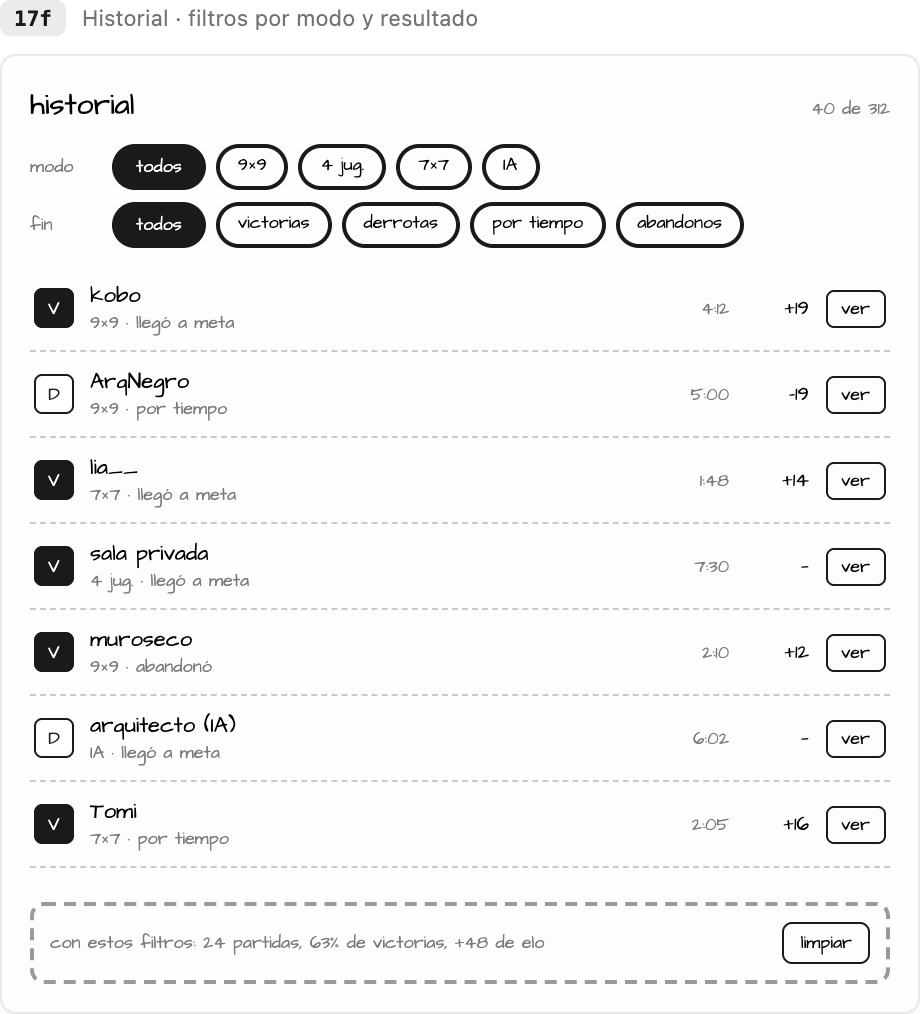
\includegraphics[width=\linewidth]{Prototipos/17f}\par\smallskip
{\footnotesize\textit{Prototipo 17f: Historial · filtros por modo y final}}
\end{minipage}
\par\medskip
\end{center}

%--- F-30 Consultar repetición de una partida
\begin{prototipocrud}{F-30}{Consultar repetición de una partida}
  \crudFila{Operación}{Consulta (R)}
  \crudFila{Caso de uso}{\mbox{CU-37}}
  \crudFila{Actor}{Jugador o moderador}
  \crudFila{Prototipos}{2f, Repetición · tablero con línea de tiempo.}
  \crudFila{Datos de entrada}{\begin{crudlista}
    \item \texttt{id\_\allowbreak{}partida}.
    \item Token de sesión.
  \end{crudlista}}
  \crudFila{Datos que se consultan}{\begin{crudlista}
    \item \textit{Partida} y \textit{Modo}: \texttt{estado}, tamaño del tablero.
    \item \textit{Participacion} y \textit{Usuario}: \texttt{orden\_\allowbreak{}turno}, \texttt{simbolo\_\allowbreak{}peon}, \texttt{nickname}, y si el jugador participó.
    \item \textit{Reporte}: para el acceso de un moderador.
    \item \textit{ParticipacionObjeto}: el aspecto de cada jugador en esa partida.
    \item \textit{Jugada}: todas, ordenadas por \texttt{numero\_\allowbreak{}jugada}, con \texttt{deshecha}.
  \end{crudlista}}
  \crudFila{Datos que se crean}{Ninguno.}
  \crudFila{Datos que se modifican}{Ninguno.}
  \crudFila{Datos que se eliminan}{Ninguno.}
  \crudFila{Reglas de negocio}{\begin{crudlista}
    \item Solo la ven sus participantes, y los moderadores si la partida está en un reporte (\mbox{CU-37} \mbox{RN-01}).
    \item El tablero se reconstruye aplicando las jugadas en orden (\mbox{CU-37} \mbox{RN-02}).
    \item La notación exportable se genera en el cliente y no se almacena (\mbox{CU-37} \mbox{RN-04}).
  \end{crudlista}}
  \crudFila{Resultado esperado}{Repetición jugada a jugada sobre el tablero, con línea de tiempo y notación exportable.}
\end{prototipocrud}
\par\nopagebreak\smallskip
\begin{center}
\begin{minipage}[t]{0.50\textwidth}\centering
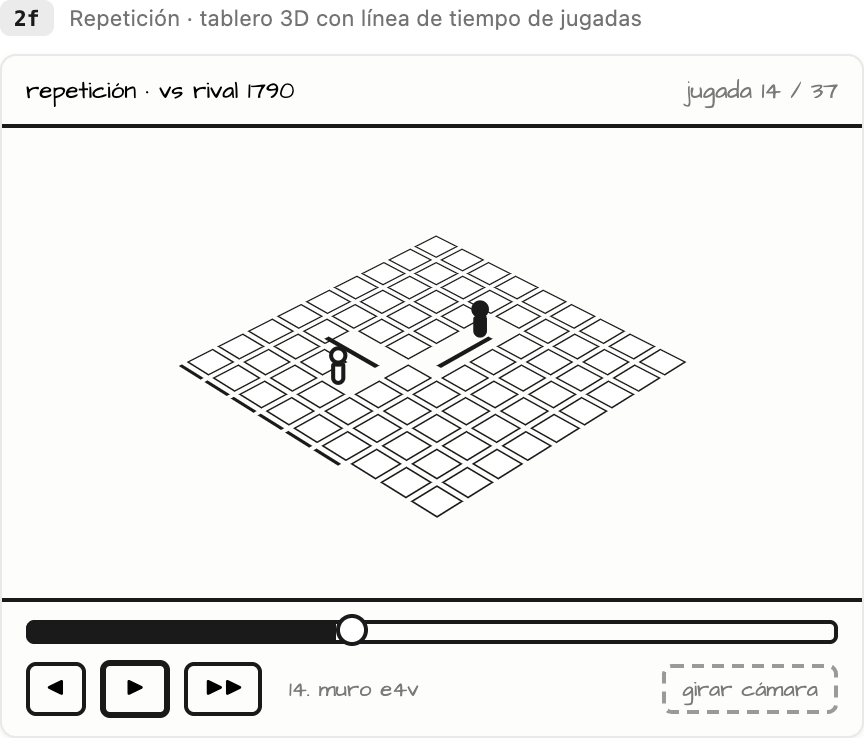
\includegraphics[width=\linewidth]{Prototipos/2f}\par\smallskip
{\footnotesize\textit{Prototipo 2f: Repetición · tablero con línea de tiempo}}
\end{minipage}
\par\medskip
\end{center}

%--- F-31 Ver una partida como espectador
\begin{prototipocrud}{F-31}{Ver una partida como espectador}
  \crudFila{Operación}{Consulta (R), Creación (C)}
  \crudFila{Caso de uso}{\mbox{CU-34}}
  \crudFila{Actor}{Jugador, invitado o anónimo}
  \crudFila{Prototipos}{10g, Espectador · con chat de espectadores; 13e, Compartir tu partida.}
  \crudFila{Datos de entrada}{\begin{crudlista}
    \item \texttt{id\_\allowbreak{}partida}, o el token de un enlace compartido.
    \item Para compartir: la orden del participante.
    \item Token de sesión, si lo hay.
  \end{crudlista}}
  \crudFila{Datos que se consultan}{\begin{crudlista}
    \item \textit{Partida}: \texttt{estado}, \texttt{tipo}.
    \item \textit{Participacion} y \textit{Usuario}: participantes y su \texttt{permite\_\allowbreak{}espectadores}.
    \item \textit{Sala}: \texttt{permite\_\allowbreak{}espectadores}, si la partida viene de una sala.
    \item \textit{Bloqueo}: entre el espectador y los participantes.
    \item \textit{Jugada} y \textit{ParticipacionObjeto}.
    \item \textit{EnlaceEspectador}: por \texttt{token\_\allowbreak{}hash}.
  \end{crudlista}}
  \crudFila{Datos que se crean}{\begin{crudlista}
    \item \textit{EnlaceEspectador}: \texttt{id\_\allowbreak{}partida}, \texttt{id\_\allowbreak{}creador}, \texttt{token\_\allowbreak{}hash}, \texttt{fecha\_\allowbreak{}creacion}, \texttt{activo} = 1, al compartir.
    \item \textit{Mensaje} con \texttt{canal} = \texttt{ESPECTADORES}, si el espectador escribe.
  \end{crudlista}}
  \crudFila{Datos que se modifican}{Ninguno.}
  \crudFila{Datos que se eliminan}{Ninguno.}
  \crudFila{Reglas de negocio}{\begin{crudlista}
    \item Los espectadores ven la partida con ocho segundos de retraso (\mbox{CU-34} \mbox{RN-01}, \mbox{D-19}).
    \item Solo si todos los participantes lo permiten (\mbox{CU-34} \mbox{RN-02}).
    \item Aforo de doscientos por partida, llevado en memoria (\mbox{CU-34} \mbox{RN-03}).
    \item Un espectador sin cuenta lee pero no escribe (\mbox{CU-34} \mbox{RN-05}).
    \item El enlace caduca al terminar la partida (\mbox{CU-34} \mbox{RN-06}).
  \end{crudlista}}
  \crudFila{Resultado esperado}{El espectador ve la partida en directo con retraso y, al terminar, puede abrir su repetición.}
\end{prototipocrud}
\par\nopagebreak\smallskip
\begin{center}
\begin{minipage}[t]{0.48\textwidth}\centering
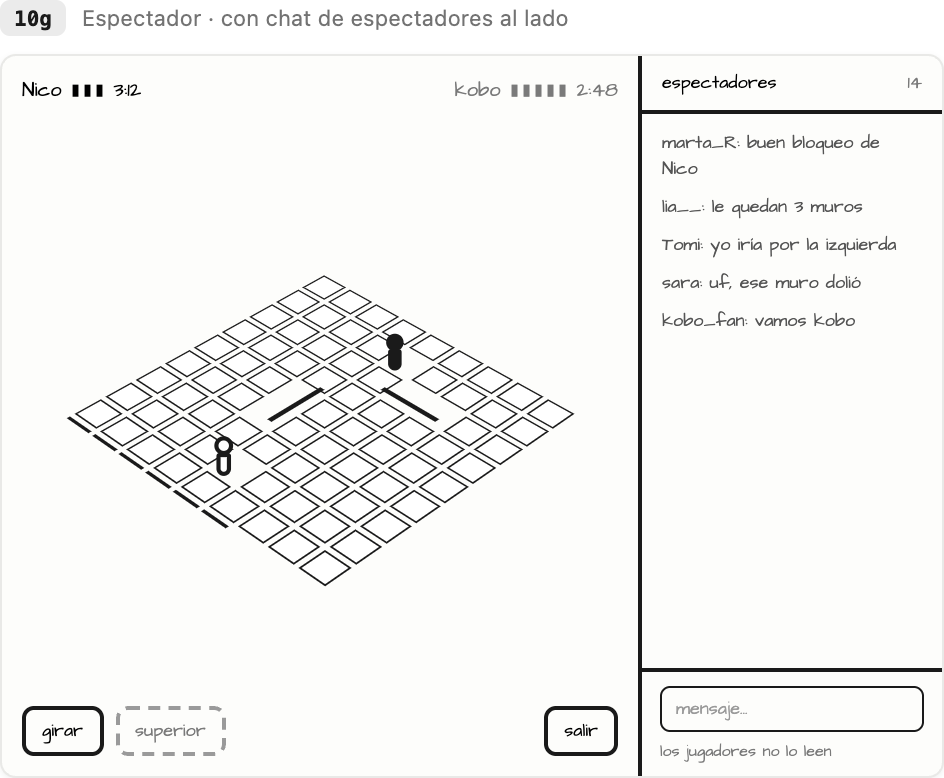
\includegraphics[width=\linewidth]{Prototipos/10g}\par\smallskip
{\footnotesize\textit{Prototipo 10g: Espectador · con chat de espectadores}}
\end{minipage}\hfill
\begin{minipage}[t]{0.48\textwidth}\centering
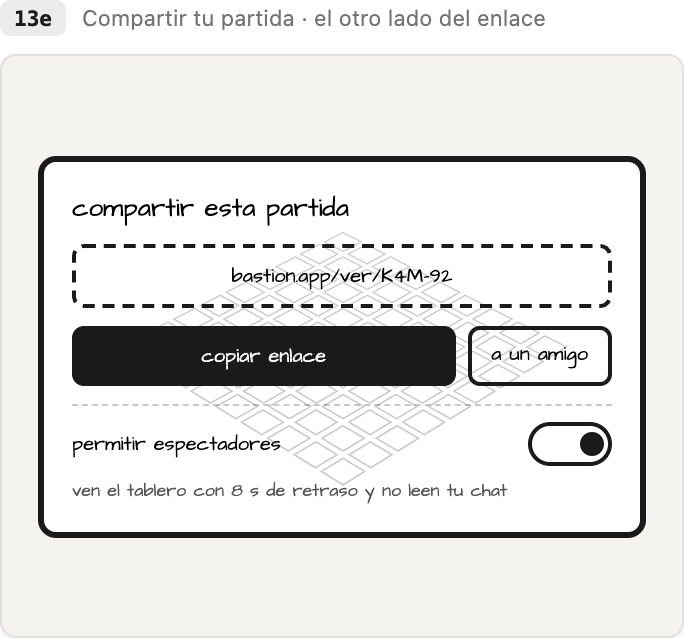
\includegraphics[width=\linewidth]{Prototipos/13e}\par\smallskip
{\footnotesize\textit{Prototipo 13e: Compartir tu partida}}
\end{minipage}
\par\medskip
\end{center}

%--- F-32 Consultar ranking
\begin{prototipocrud}{F-32}{Consultar ranking}
  \crudFila{Operación}{Consulta (R)}
  \crudFila{Caso de uso}{\mbox{CU-35}}
  \crudFila{Actor}{Jugador o invitado}
  \crudFila{Prototipos}{2c, Ranking · tabla con tu fila fijada; 2d, Ranking · divisiones con top 3.}
  \crudFila{Datos de entrada}{\begin{crudlista}
    \item Alcance: global o entre amigos.
    \item \texttt{id\_\allowbreak{}modo}.
    \item Búsqueda opcional por \texttt{nickname} o \texttt{codigo\_\allowbreak{}amigo}.
    \item Vista: tabla o divisiones.
    \item Página solicitada.
  \end{crudlista}}
  \crudFila{Datos que se consultan}{\begin{crudlista}
    \item \textit{EstadisticaModo}: \texttt{puntos\_\allowbreak{}elo}, \texttt{division}, \texttt{partidas\_\allowbreak{}jugadas}.
    \item \textit{Usuario}: \texttt{nickname}, \texttt{id\_\allowbreak{}icono}, \texttt{codigo\_\allowbreak{}amigo}, \texttt{estado\_\allowbreak{}cuenta}.
    \item \textit{Division}: para la vista por divisiones.
    \item \textit{Amistad}: para el alcance entre amigos.
    \item \textit{Bloqueo}: para la búsqueda.
  \end{crudlista}}
  \crudFila{Datos que se crean}{Ninguno.}
  \crudFila{Datos que se modifican}{Ninguno.}
  \crudFila{Datos que se eliminan}{Ninguno.}
  \crudFila{Reglas de negocio}{\begin{crudlista}
    \item Hacen falta cinco partidas en un modo para clasificar (\mbox{CU-35} \mbox{RN-01}).
    \item Solo aparecen cuentas \texttt{ACTIVA} (\mbox{CU-35} \mbox{RN-02}).
    \item La búsqueda no devuelve a jugadores con bloqueo (\mbox{CU-35} \mbox{RN-04}).
    \item No hay temporadas (\mbox{CU-35} \mbox{RN-07}).
  \end{crudlista}}
  \crudFila{Resultado esperado}{Clasificación ordenada por elo con la posición del jugador fijada, o los resultados de la búsqueda.}
\end{prototipocrud}
\par\nopagebreak\smallskip
\begin{center}
\begin{minipage}[t]{0.48\textwidth}\centering
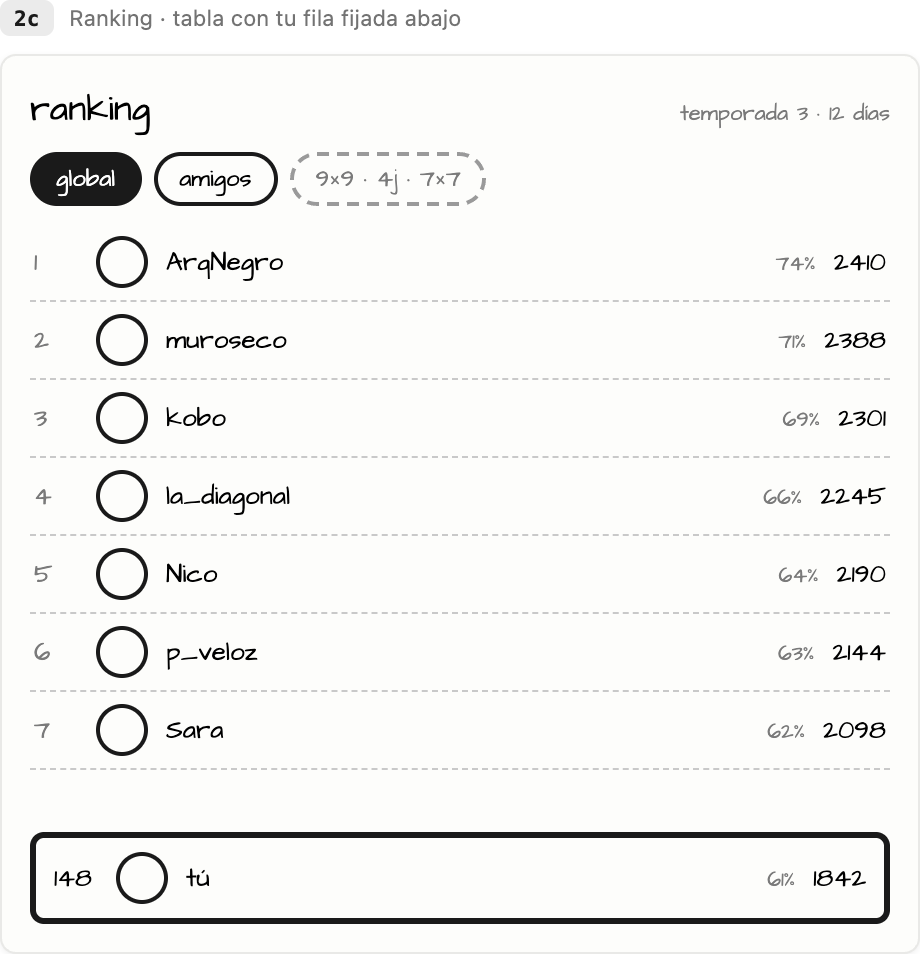
\includegraphics[width=\linewidth]{Prototipos/2c}\par\smallskip
{\footnotesize\textit{Prototipo 2c: Ranking · tabla con tu fila fijada}}
\end{minipage}\hfill
\begin{minipage}[t]{0.48\textwidth}\centering
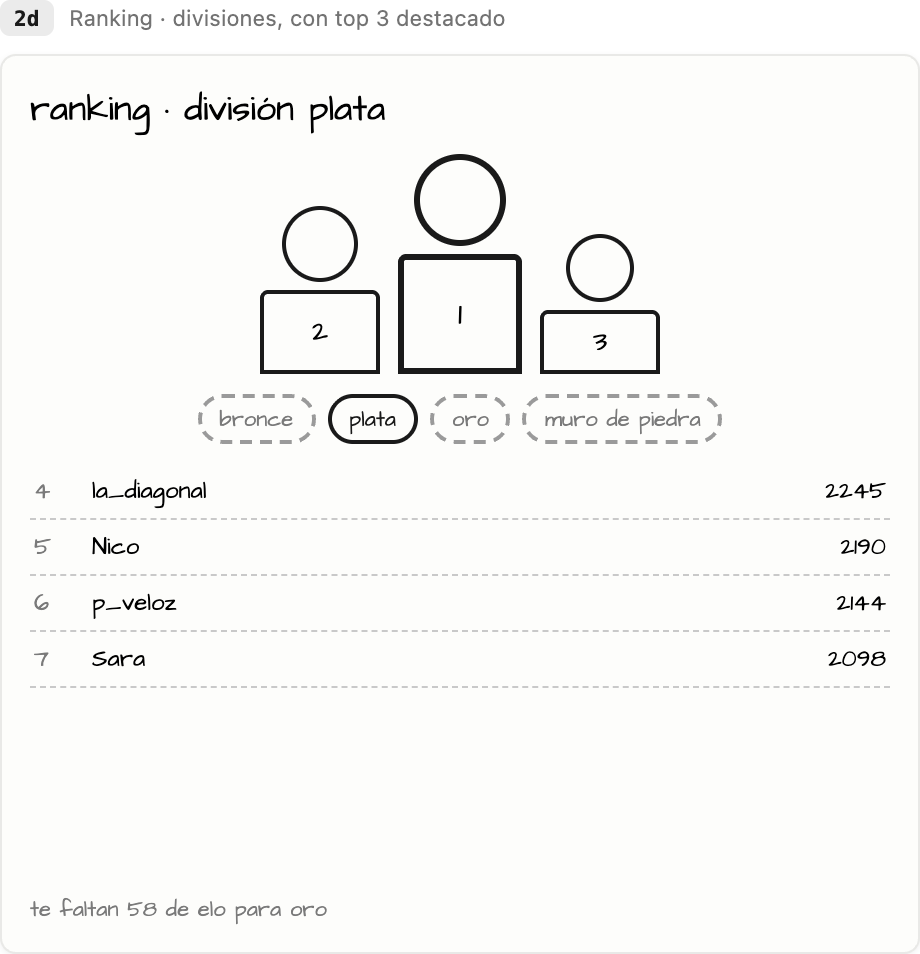
\includegraphics[width=\linewidth]{Prototipos/2d}\par\smallskip
{\footnotesize\textit{Prototipo 2d: Ranking · divisiones con top 3}}
\end{minipage}
\par\medskip
\end{center}

\subsection*{Aprendizaje}
\addcontentsline{toc}{subsection}{Aprendizaje}

El tutorial es la única funcionalidad del sistema en la que el servidor no valida lo que ocurre en el tablero, porque no hay nada en juego (\mbox{D-18}).

%--- F-33 Avanzar en el tutorial
\begin{prototipocrud}{F-33}{Avanzar en el tutorial}
  \crudFila{Operación}{Creación (C), Actualización (U)}
  \crudFila{Caso de uso}{\mbox{CU-41}}
  \crudFila{Actor}{Jugador o invitado}
  \crudFila{Prototipos}{6b, Tutorial · índice de lecciones; 6a, Tutorial · pasos sobre el tablero.}
  \crudFila{Datos de entrada}{\begin{crudlista}
    \item \texttt{id\_\allowbreak{}leccion}.
    \item Número de paso completado.
    \item Token de sesión.
  \end{crudlista}}
  \crudFila{Datos que se consultan}{\begin{crudlista}
    \item \textit{Leccion}: \texttt{orden}, \texttt{nombre}, \texttt{num\_\allowbreak{}pasos}.
    \item \textit{ProgresoTutorial}: el del jugador en cada lección.
  \end{crudlista}}
  \crudFila{Datos que se crean}{\begin{crudlista}
    \item \textit{ProgresoTutorial}: \texttt{id\_\allowbreak{}usuario}, \texttt{id\_\allowbreak{}leccion}, \texttt{paso\_\allowbreak{}actual}, \texttt{completada} = 0, \texttt{fecha\_\allowbreak{}actualizacion}, al completar el primer paso de una lección.
  \end{crudlista}}
  \crudFila{Datos que se modifican}{\begin{crudlista}
    \item \textit{ProgresoTutorial}: \texttt{paso\_\allowbreak{}actual} y \texttt{fecha\_\allowbreak{}actualizacion} en cada paso; \texttt{completada} = 1 y \texttt{fecha\_\allowbreak{}completada} al terminar.
  \end{crudlista}}
  \crudFila{Datos que se eliminan}{Ninguno.}
  \crudFila{Reglas de negocio}{\begin{crudlista}
    \item Siete lecciones sobre el tablero real (\mbox{CU-41} \mbox{RN-01}).
    \item La acción se valida en el cliente y el tutorial funciona sin conexión (\mbox{CU-41} \mbox{RN-02}).
    \item El progreso se guarda en la cuenta, paso a paso (\mbox{CU-41} \mbox{RN-03}).
    \item Repetir una lección completada no cambia su progreso (\mbox{CU-41} \mbox{RN-04}).
    \item No otorga experiencia, monedas ni objetos (\mbox{CU-41} \mbox{RN-05}).
  \end{crudlista}}
  \crudFila{Resultado esperado}{El avance del jugador queda guardado y puede continuar la lección en cualquier dispositivo.}
\end{prototipocrud}
\par\nopagebreak\smallskip
\begin{center}
\begin{minipage}[t]{0.48\textwidth}\centering
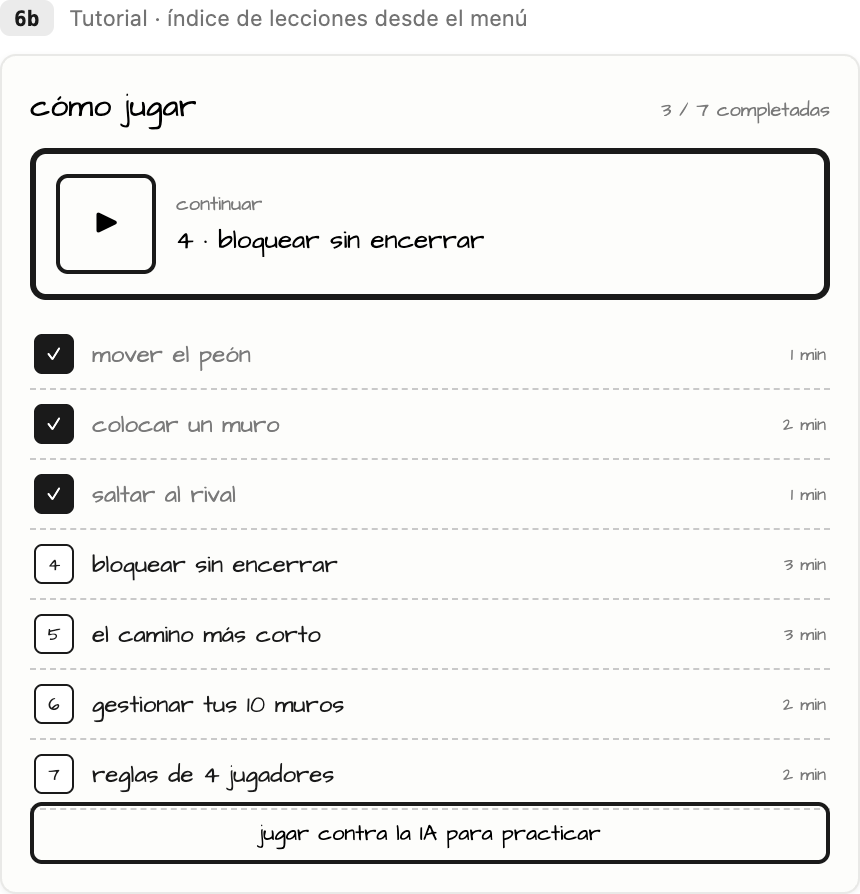
\includegraphics[width=\linewidth]{Prototipos/6b}\par\smallskip
{\footnotesize\textit{Prototipo 6b: Tutorial · índice de lecciones}}
\end{minipage}\hfill
\begin{minipage}[t]{0.48\textwidth}\centering
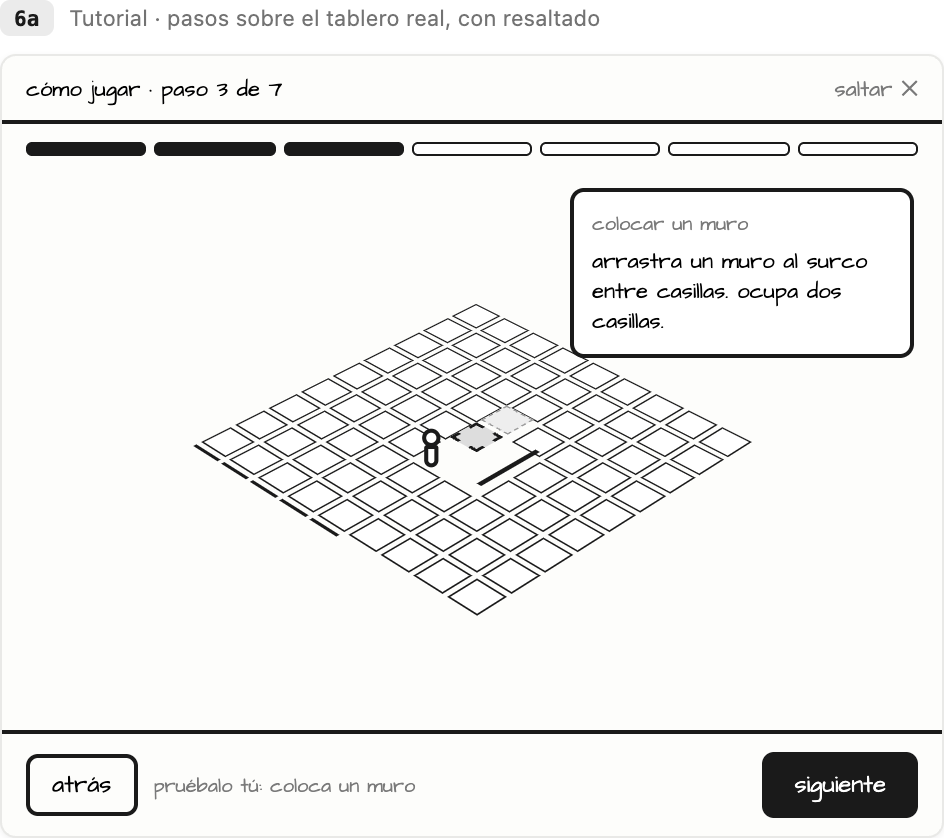
\includegraphics[width=\linewidth]{Prototipos/6a}\par\smallskip
{\footnotesize\textit{Prototipo 6a: Tutorial · pasos sobre el tablero}}
\end{minipage}
\par\medskip
\end{center}

\subsection*{Personalización y economía}
\addcontentsline{toc}{subsection}{Personalización y economía}

Todo lo que se compra es cosmético y se paga solo con monedas del juego. La posesión y el equipamiento son estructuras distintas: poseer un objeto no lo equipa, y equiparlo no lo otorga.

%--- F-34 Comprar un objeto
\begin{prototipocrud}{F-34}{Comprar un objeto}
  \crudFila{Operación}{Creación (C)}
  \crudFila{Caso de uso}{\mbox{CU-38}}
  \crudFila{Actor}{Jugador o invitado}
  \crudFila{Prototipos}{4d, Tienda · destacado y rejilla; 4f, Tienda · confirmación de compra.}
  \crudFila{Datos de entrada}{\begin{crudlista}
    \item \texttt{id\_\allowbreak{}objeto}.
    \item Precio mostrado por el cliente.
    \item Token de sesión.
  \end{crudlista}}
  \crudFila{Datos que se consultan}{\begin{crudlista}
    \item \textit{ObjetoCosmetico}: \texttt{precio}, \texttt{a\_\allowbreak{}la\_\allowbreak{}venta}, \texttt{activo}, \texttt{nivel\_\allowbreak{}requerido}.
    \item \textit{UsuarioObjeto}: que el usuario no lo posea ya.
    \item \textit{Usuario}: \texttt{saldo\_\allowbreak{}monedas}, \texttt{nivel}.
  \end{crudlista}}
  \crudFila{Datos que se crean}{\begin{crudlista}
    \item \textit{UsuarioObjeto}: \texttt{fecha\_\allowbreak{}obtencion}, \texttt{origen} = \texttt{COMPRA}.
    \item \textit{MovimientoMoneda}: \texttt{tipo} = \texttt{COMPRA}, \texttt{importe} negativo, \texttt{id\_\allowbreak{}objeto}, \texttt{fecha\_\allowbreak{}movimiento}.
  \end{crudlista}}
  \crudFila{Datos que se modifican}{\begin{crudlista}
    \item \textit{Usuario}: \texttt{saldo\_\allowbreak{}monedas}.
  \end{crudlista}}
  \crudFila{Datos que se eliminan}{Ninguno.}
  \crudFila{Reglas de negocio}{\begin{crudlista}
    \item Solo se paga con monedas del juego; no existe dinero real (\mbox{CU-38} \mbox{RN-01}).
    \item Un objeto no puede poseerse dos veces (\mbox{CU-38} \mbox{RN-02}).
    \item El precio válido es el del servidor (\mbox{CU-38} \mbox{RN-03}).
    \item Un objeto bloqueado por nivel no se vende aunque haya saldo (\mbox{CU-38} \mbox{RN-04}).
    \item El saldo debe coincidir con la suma de los movimientos (\mbox{CU-38} \mbox{RN-05}).
  \end{crudlista}}
  \crudFila{Resultado esperado}{El jugador posee el objeto, su saldo disminuyó en el precio y el movimiento quedó registrado.}
\end{prototipocrud}
\par\nopagebreak\smallskip
\begin{center}
\begin{minipage}[t]{0.48\textwidth}\centering
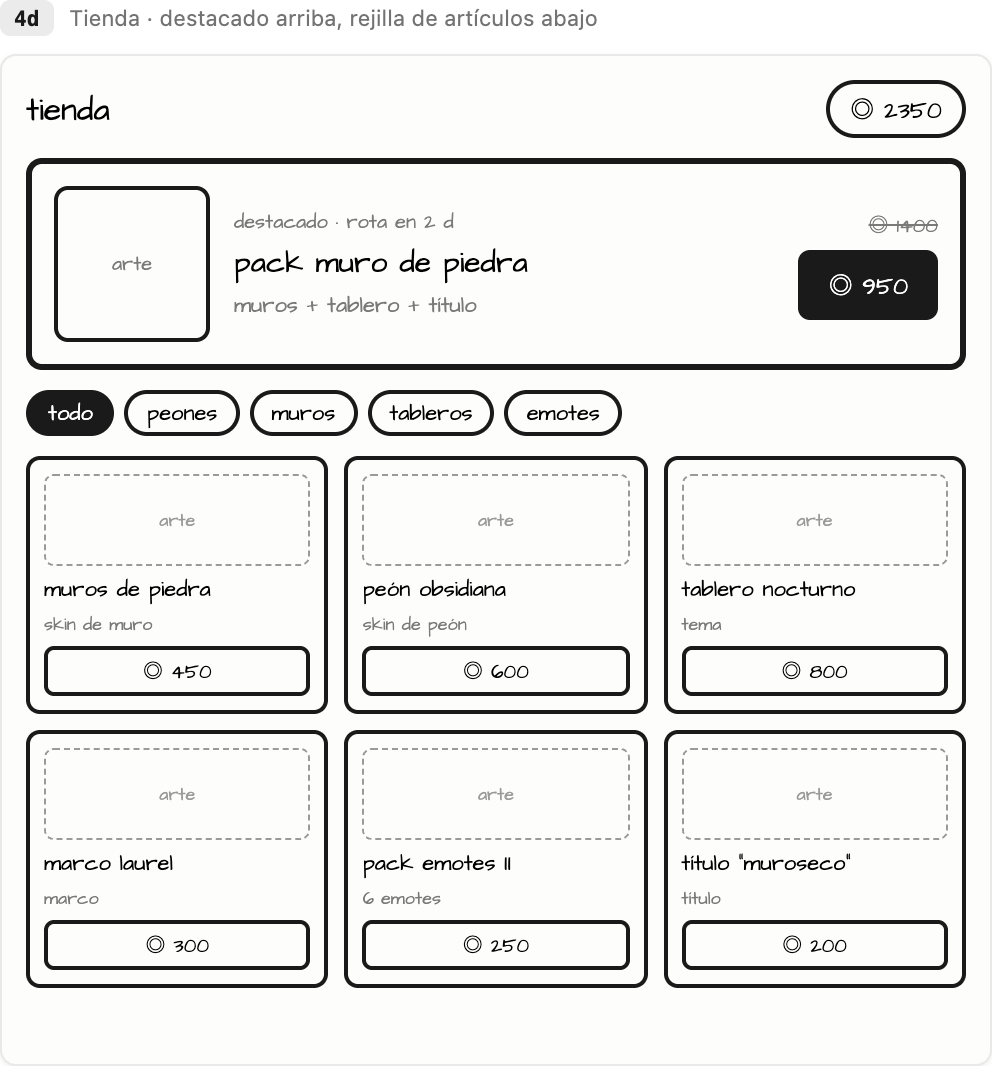
\includegraphics[width=\linewidth]{Prototipos/4d}\par\smallskip
{\footnotesize\textit{Prototipo 4d: Tienda · destacado y rejilla}}
\end{minipage}\hfill
\begin{minipage}[t]{0.48\textwidth}\centering
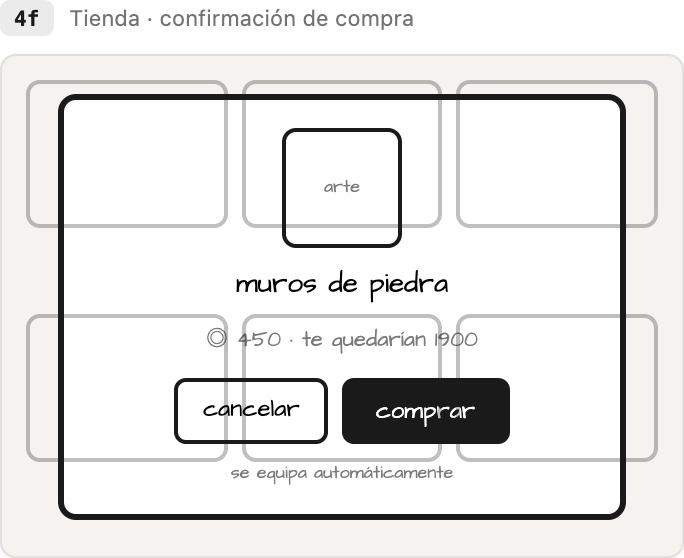
\includegraphics[width=\linewidth]{Prototipos/4f}\par\smallskip
{\footnotesize\textit{Prototipo 4f: Tienda · confirmación de compra}}
\end{minipage}
\par\medskip
\end{center}

%--- F-35 Comprar y abrir una caja
\begin{prototipocrud}{F-35}{Comprar y abrir una caja}
  \crudFila{Operación}{Creación (C), Actualización (U)}
  \crudFila{Caso de uso}{\mbox{CU-39}}
  \crudFila{Actor}{Jugador o invitado}
  \crudFila{Prototipos}{14d, Contenido y probabilidades; 14e, Confirmar compra de caja; 14c, Resultado de la caja.}
  \crudFila{Datos de entrada}{\begin{crudlista}
    \item Para comprar: \texttt{id\_\allowbreak{}tipo\_\allowbreak{}caja} y el precio mostrado.
    \item Para abrir: \texttt{id\_\allowbreak{}caja}.
    \item Token de sesión.
  \end{crudlista}}
  \crudFila{Datos que se consultan}{\begin{crudlista}
    \item \textit{TipoCaja}: \texttt{precio}, \texttt{activo}.
    \item \textit{TipoCajaObjeto}: \texttt{id\_\allowbreak{}objeto} y \texttt{probabilidad} de cada objeto posible.
    \item \textit{UsuarioObjeto}: para detectar repetidos.
    \item \textit{Usuario}: \texttt{saldo\_\allowbreak{}monedas}, \texttt{cajas\_\allowbreak{}sin\_\allowbreak{}raro}.
    \item \textit{Caja}: \texttt{estado}, \texttt{origen}, \texttt{fecha\_\allowbreak{}caducidad}.
  \end{crudlista}}
  \crudFila{Datos que se crean}{\begin{crudlista}
    \item \textit{Caja}: \texttt{id\_\allowbreak{}tipo\_\allowbreak{}caja}, \texttt{origen} = \texttt{COMPRA}, \texttt{estado} = \texttt{SIN\_\allowbreak{}ABRIR}, \texttt{fecha\_\allowbreak{}obtencion}.
    \item \textit{MovimientoMoneda}: \texttt{COMPRA\_\allowbreak{}CAJA} al comprar, \texttt{CONVERSION} por cada repetido y \texttt{DEVOLUCION} si la caja cobrada no llega a crearse.
    \item \textit{UsuarioObjeto}: los objetos nuevos, con \texttt{origen} = \texttt{CAJA}.
    \item \textit{CajaContenido}: tres filas con \texttt{id\_\allowbreak{}objeto}, \texttt{convertido} y \texttt{monedas\_\allowbreak{}conversion}.
  \end{crudlista}}
  \crudFila{Datos que se modifican}{\begin{crudlista}
    \item \textit{Usuario}: \texttt{saldo\_\allowbreak{}monedas}, \texttt{cajas\_\allowbreak{}sin\_\allowbreak{}raro}.
    \item \textit{Caja}: \texttt{estado} = \texttt{ABIERTA} y \texttt{fecha\_\allowbreak{}apertura}, o \texttt{CADUCADA}.
  \end{crudlista}}
  \crudFila{Datos que se eliminan}{Ninguno.}
  \crudFila{Reglas de negocio}{\begin{crudlista}
    \item Las probabilidades se muestran antes de comprar (\mbox{CU-39} \mbox{RN-01}).
    \item Los repetidos se convierten en monedas automáticamente (\mbox{CU-39} \mbox{RN-03}).
    \item A las diez cajas sin objeto raro, la siguiente lo garantiza (\mbox{CU-39} \mbox{RN-05}).
    \item Las cajas ganadas jugando caducan a los catorce días; las compradas no (\mbox{CU-39} \mbox{RN-06}).
    \item El sorteo lo hace el servidor (\mbox{CU-39} \mbox{RN-08}).
  \end{crudlista}}
  \crudFila{Resultado esperado}{El jugador obtuvo tres objetos o su equivalente en monedas, con el contenido de la caja registrado y el contador de garantía actualizado.}
\end{prototipocrud}
\par\nopagebreak\smallskip
\begin{center}
\begin{minipage}[t]{0.48\textwidth}\centering
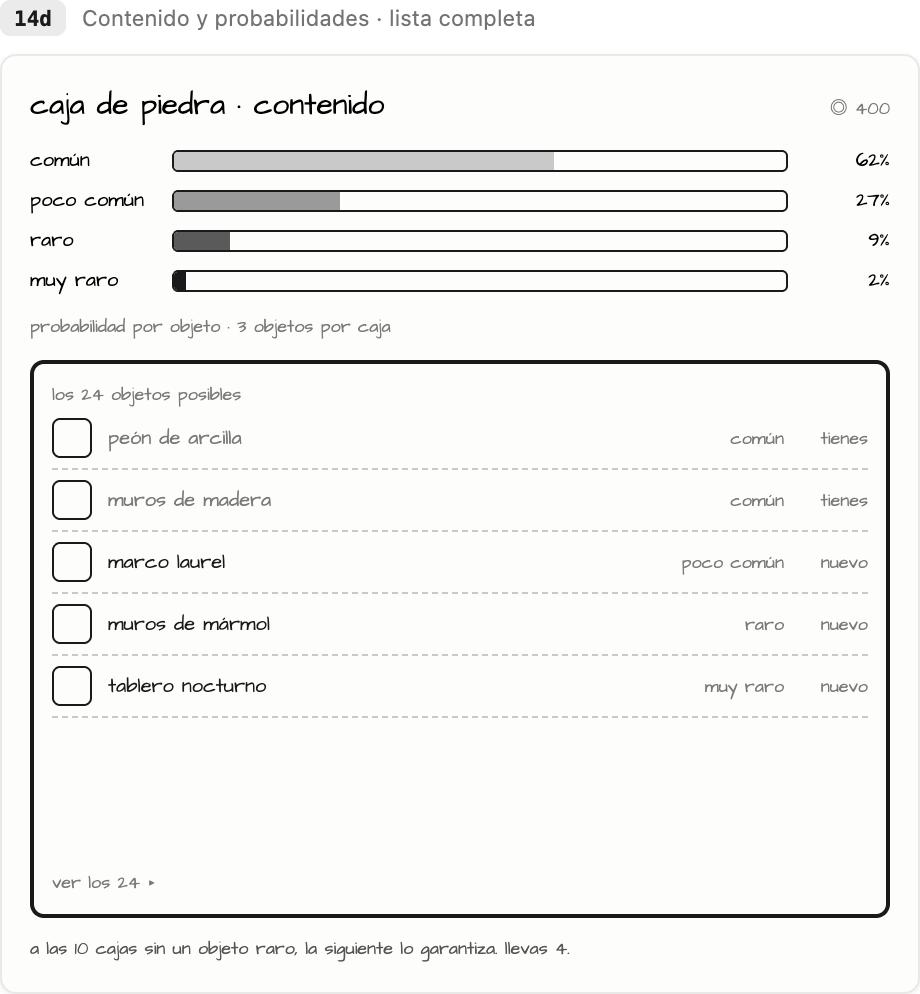
\includegraphics[width=\linewidth]{Prototipos/14d}\par\smallskip
{\footnotesize\textit{Prototipo 14d: Contenido y probabilidades}}
\end{minipage}\hfill
\begin{minipage}[t]{0.48\textwidth}\centering
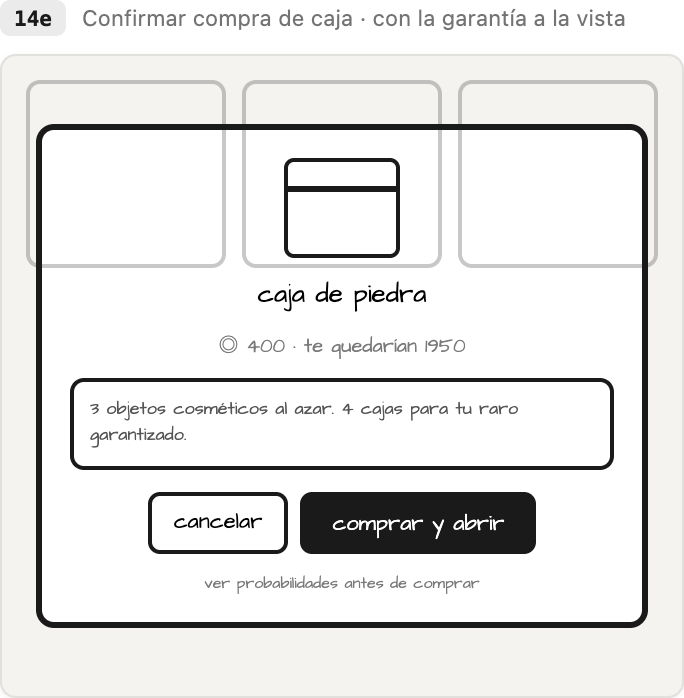
\includegraphics[width=\linewidth]{Prototipos/14e}\par\smallskip
{\footnotesize\textit{Prototipo 14e: Confirmar compra de caja}}
\end{minipage}
\par\medskip
\begin{minipage}[t]{0.50\textwidth}\centering
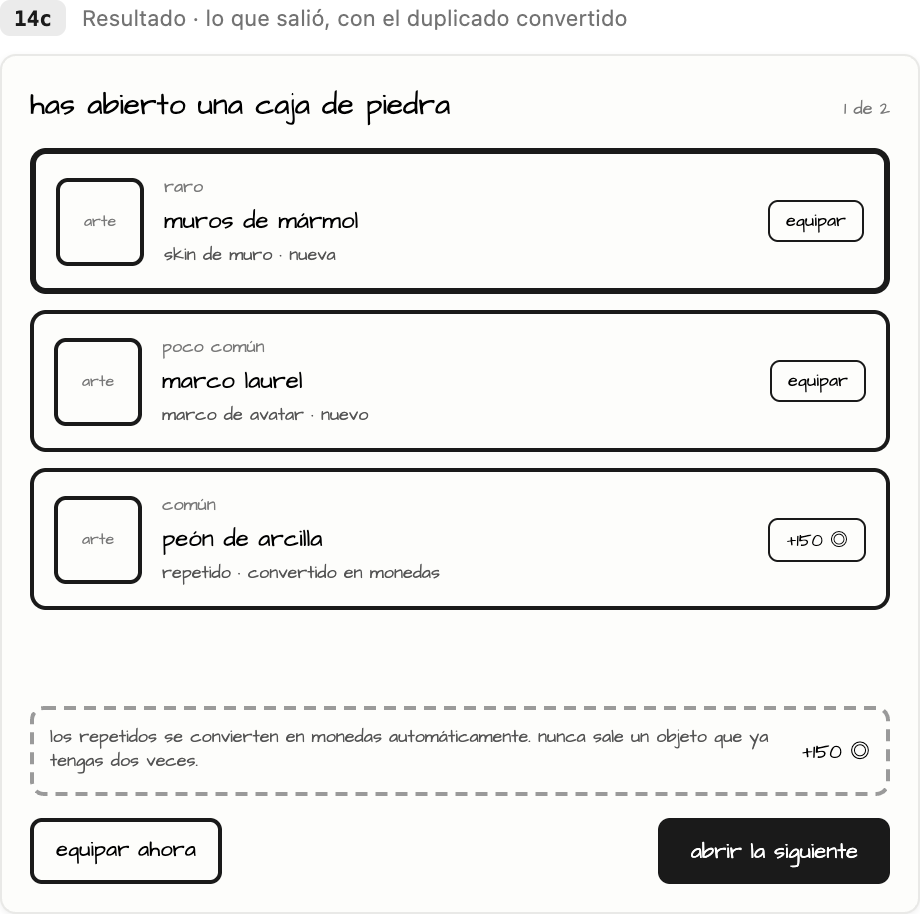
\includegraphics[width=\linewidth]{Prototipos/14c}\par\smallskip
{\footnotesize\textit{Prototipo 14c: Resultado de la caja}}
\end{minipage}
\par\medskip
\end{center}

%--- F-36 Equipar un objeto
\begin{prototipocrud}{F-36}{Equipar un objeto}
  \crudFila{Operación}{Actualización (U)}
  \crudFila{Caso de uso}{\mbox{CU-14}}
  \crudFila{Actor}{Jugador o invitado}
  \crudFila{Prototipos}{4a, Personalizar · vista previa 3D y rejilla.}
  \crudFila{Datos de entrada}{\begin{crudlista}
    \item \texttt{id\_\allowbreak{}objeto}.
    \item Token de sesión.
  \end{crudlista}}
  \crudFila{Datos que se consultan}{\begin{crudlista}
    \item \textit{ObjetoCosmetico}: \texttt{id\_\allowbreak{}ranura}, \texttt{activo}.
    \item \textit{UsuarioObjeto}: que el usuario lo posea.
  \end{crudlista}}
  \crudFila{Datos que se crean}{Ninguno.}
  \crudFila{Datos que se modifican}{\begin{crudlista}
    \item \textit{Equipamiento}: la fila (\texttt{id\_\allowbreak{}usuario}, \texttt{id\_\allowbreak{}ranura}) pasa a apuntar al \texttt{id\_\allowbreak{}objeto} elegido.
  \end{crudlista}}
  \crudFila{Datos que se eliminan}{Ninguno.}
  \crudFila{Reglas de negocio}{\begin{crudlista}
    \item Cada usuario tiene exactamente un objeto equipado por ranura, siempre (\mbox{CU-14} \mbox{RN-01}).
    \item Solo se equipa lo que se posee (\mbox{CU-14} \mbox{RN-02}).
    \item El cambio no afecta a una partida en curso (\mbox{CU-14} \mbox{RN-03}).
    \item Un objeto retirado del catálogo se conserva equipado hasta que el jugador lo cambie (\mbox{CU-14} \mbox{RN-04}).
  \end{crudlista}}
  \crudFila{Resultado esperado}{El objeto queda equipado en su ranura; las otras cinco no cambian.}
\end{prototipocrud}
\par\nopagebreak\smallskip
\begin{center}
\begin{minipage}[t]{0.50\textwidth}\centering
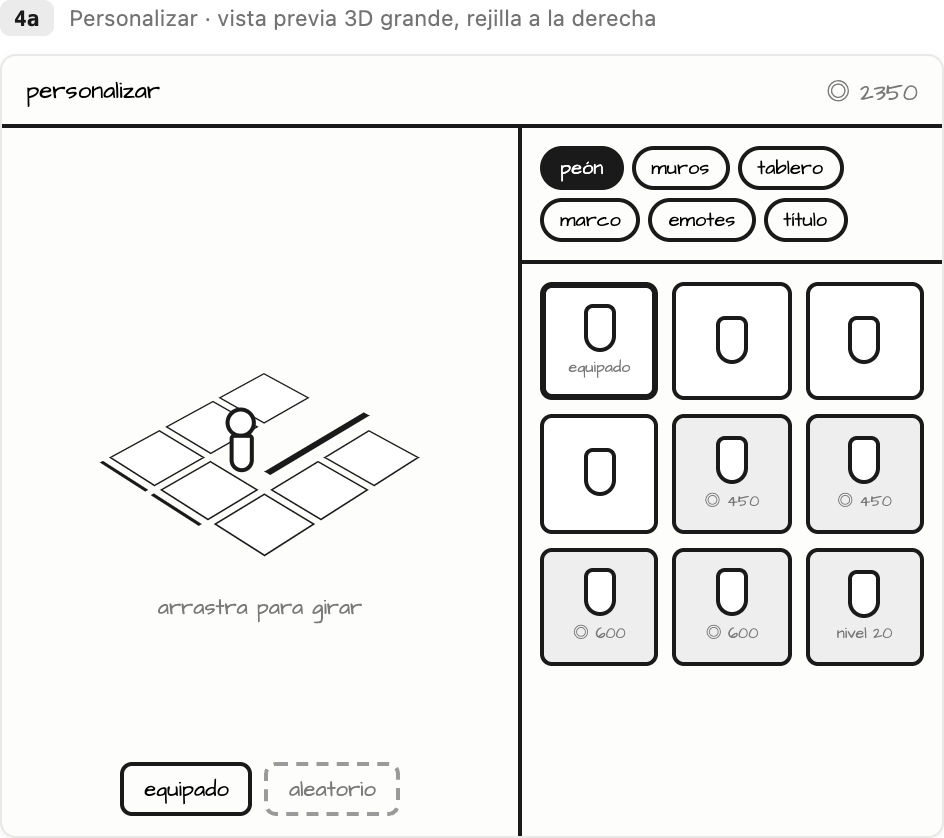
\includegraphics[width=\linewidth]{Prototipos/4a}\par\smallskip
{\footnotesize\textit{Prototipo 4a: Personalizar · vista previa 3D y rejilla}}
\end{minipage}
\par\medskip
\end{center}

%--- F-37 Consultar inventario y tienda
\begin{prototipocrud}{F-37}{Consultar inventario y tienda}
  \crudFila{Operación}{Consulta (R)}
  \crudFila{Caso de uso}{\mbox{CU-14}, \mbox{CU-38}}
  \crudFila{Actor}{Jugador o invitado}
  \crudFila{Prototipos}{4c, Personalizar · lista de ranuras equipadas.}
  \crudFila{Datos de entrada}{\begin{crudlista}
    \item \texttt{id\_\allowbreak{}ranura}, como filtro opcional.
    \item Token de sesión.
  \end{crudlista}}
  \crudFila{Datos que se consultan}{\begin{crudlista}
    \item \textit{Ranura}: las seis.
    \item \textit{ObjetoCosmetico}: \texttt{nombre}, \texttt{rareza}, \texttt{precio}, \texttt{nivel\_\allowbreak{}requerido}, \texttt{a\_\allowbreak{}la\_\allowbreak{}venta}, \texttt{activo}.
    \item \textit{UsuarioObjeto}: lo que posee el usuario.
    \item \textit{Equipamiento}: lo que tiene equipado.
    \item \textit{TipoCaja} y \textit{Caja}: las cajas a la venta y las que el usuario tiene sin abrir.
    \item \textit{Usuario}: \texttt{saldo\_\allowbreak{}monedas}, \texttt{nivel}, \texttt{cajas\_\allowbreak{}sin\_\allowbreak{}raro}.
  \end{crudlista}}
  \crudFila{Datos que se crean}{Ninguno.}
  \crudFila{Datos que se modifican}{Ninguno.}
  \crudFila{Datos que se eliminan}{Ninguno.}
  \crudFila{Reglas de negocio}{\begin{crudlista}
    \item Se muestran también los objetos no poseídos, con su precio o su nivel requerido (\mbox{CU-14} \mbox{RN-06}).
    \item Todo el contenido es cosmético (\mbox{CU-14} \mbox{RN-05}).
  \end{crudlista}}
  \crudFila{Resultado esperado}{Rejilla de objetos por ranura que distingue lo equipado, lo poseído, lo comprable y lo bloqueado, junto con las cajas disponibles.}
\end{prototipocrud}
\par\nopagebreak\smallskip
\begin{center}
\begin{minipage}[t]{0.50\textwidth}\centering
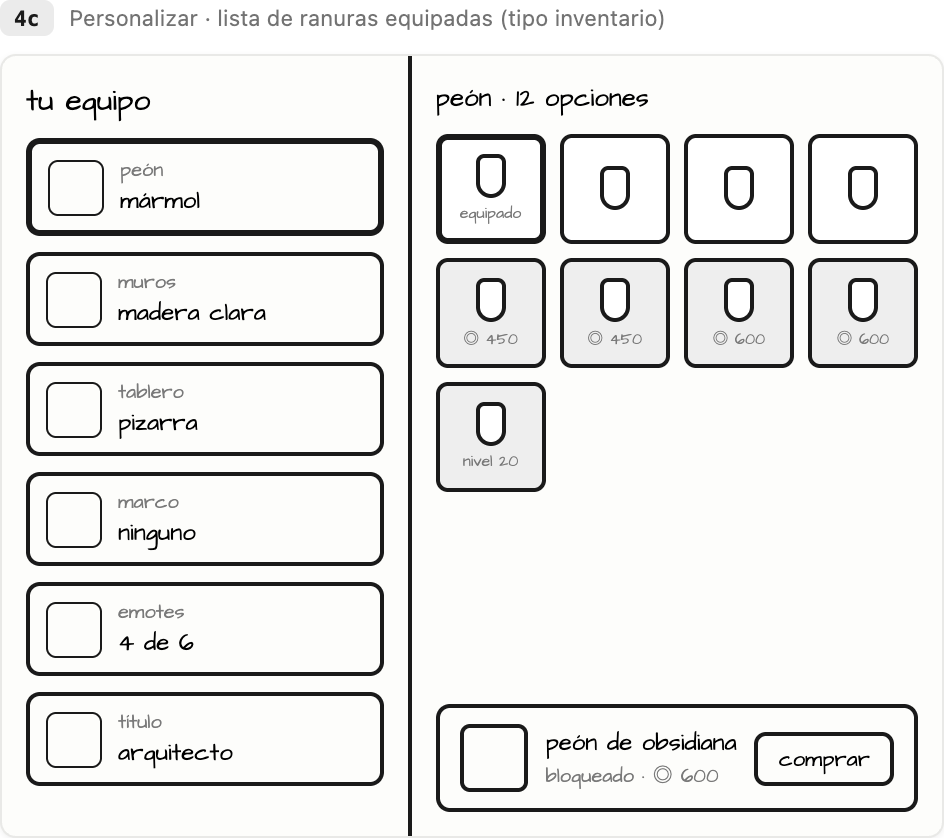
\includegraphics[width=\linewidth]{Prototipos/4c}\par\smallskip
{\footnotesize\textit{Prototipo 4c: Personalizar · lista de ranuras equipadas}}
\end{minipage}
\par\medskip
\end{center}

%--- F-38 Consultar historial de monedas
\begin{prototipocrud}{F-38}{Consultar historial de monedas}
  \crudFila{Operación}{Consulta (R)}
  \crudFila{Caso de uso}{\mbox{CU-40}}
  \crudFila{Actor}{Jugador o invitado}
  \crudFila{Prototipos}{16e, Historial de monedas.}
  \crudFila{Datos de entrada}{\begin{crudlista}
    \item Filtro opcional: ingresos, gastos o conversiones.
    \item Página solicitada.
    \item Token de sesión.
  \end{crudlista}}
  \crudFila{Datos que se consultan}{\begin{crudlista}
    \item \textit{MovimientoMoneda}: \texttt{tipo}, \texttt{importe}, \texttt{fecha\_\allowbreak{}movimiento}, \texttt{id\_\allowbreak{}objeto}, \texttt{id\_\allowbreak{}partida}, \texttt{id\_\allowbreak{}caja}, y la suma de todos los del usuario.
    \item \textit{ObjetoCosmetico}, \textit{Caja}, \textit{TipoCaja}, \textit{CajaContenido}, \textit{Partida} y \textit{Modo}: para describir cada movimiento.
    \item \textit{Usuario}: \texttt{saldo\_\allowbreak{}monedas}, para comprobar que coincide con la suma.
  \end{crudlista}}
  \crudFila{Datos que se crean}{Ninguno.}
  \crudFila{Datos que se modifican}{Ninguno.}
  \crudFila{Datos que se eliminan}{Ninguno.}
  \crudFila{Reglas de negocio}{\begin{crudlista}
    \item Los movimientos nunca se modifican ni se eliminan: una corrección es un movimiento nuevo (\mbox{CU-40} \mbox{RN-01}).
    \item El saldo verdadero es la suma de los movimientos; si \texttt{saldo\_\allowbreak{}monedas} discrepa, se muestra la suma y se registra la incidencia (\mbox{CU-40} \mbox{RN-02}, \mbox{RN-03}).
  \end{crudlista}}
  \crudFila{Resultado esperado}{Lista de ingresos, gastos y conversiones con su origen, y un saldo que coincide con ellos.}
\end{prototipocrud}
\par\nopagebreak\smallskip
\begin{center}
\begin{minipage}[t]{0.50\textwidth}\centering
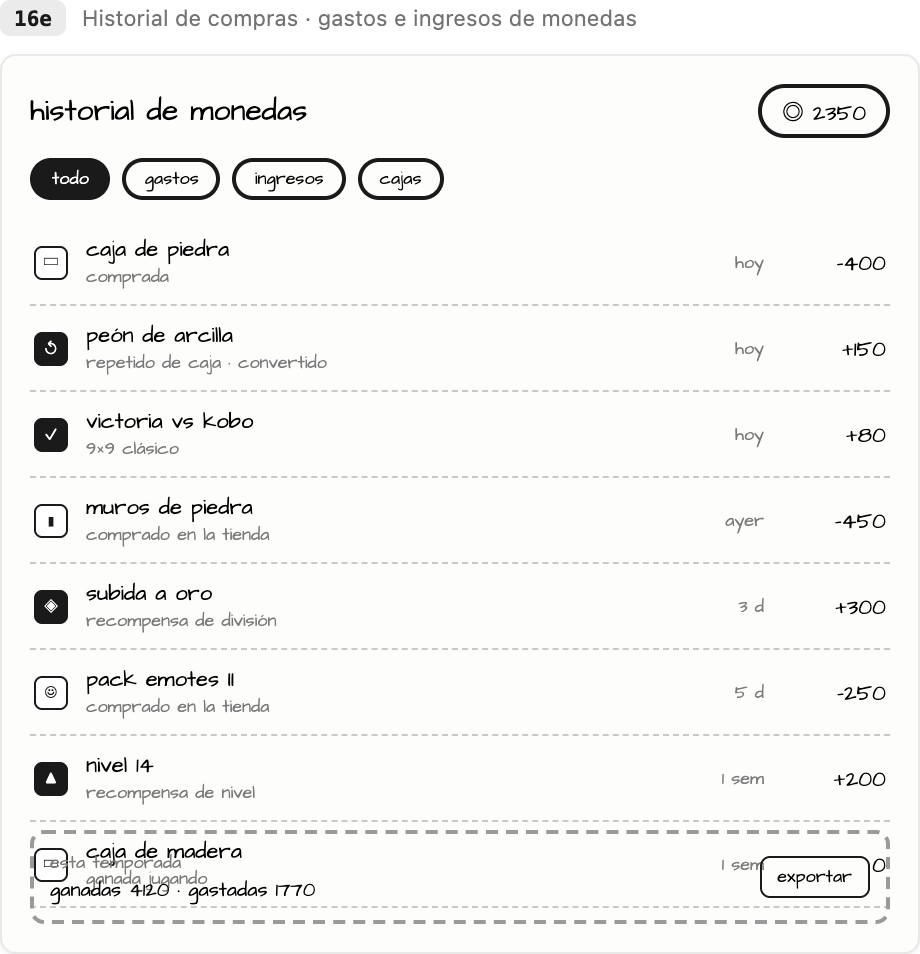
\includegraphics[width=\linewidth]{Prototipos/16e}\par\smallskip
{\footnotesize\textit{Prototipo 16e: Historial de monedas}}
\end{minipage}
\par\medskip
\end{center}

\subsection*{Relaciones entre jugadores}
\addcontentsline{toc}{subsection}{Relaciones entre jugadores}

Amistades, solicitudes, silencios y bloqueos son las únicas estructuras del sistema que se eliminan físicamente desde la aplicación: representan un estado presente de la relación y no un hecho histórico que deba conservarse.

%--- F-39 Enviar solicitud de amistad
\begin{prototipocrud}{F-39}{Enviar solicitud de amistad}
  \crudFila{Operación}{Creación (C)}
  \crudFila{Caso de uso}{\mbox{CU-30}}
  \crudFila{Actor}{Jugador con cuenta registrada}
  \crudFila{Prototipos}{10a, Menú de un jugador.}
  \crudFila{Datos de entrada}{\begin{crudlista}
    \item \texttt{nickname} o \texttt{codigo\_\allowbreak{}amigo} para buscar.
    \item \texttt{id\_\allowbreak{}usuario} del destinatario.
    \item Token de sesión.
  \end{crudlista}}
  \crudFila{Datos que se consultan}{\begin{crudlista}
    \item \textit{Usuario}: \texttt{nickname}, \texttt{codigo\_\allowbreak{}amigo}, \texttt{estado\_\allowbreak{}cuenta}.
    \item \textit{Bloqueo}: entre ambos.
    \item \textit{Amistad}: si ya son amigos, y cuántos amigos tiene cada uno.
    \item \textit{Solicitud}: pendientes en cualquier sentido.
    \item \textit{Participacion}: rivales recientes, para las sugerencias.
  \end{crudlista}}
  \crudFila{Datos que se crean}{\begin{crudlista}
    \item \textit{Solicitud}: \texttt{id\_\allowbreak{}solicitante}, \texttt{id\_\allowbreak{}destinatario}, \texttt{fecha\_\allowbreak{}solicitud}.
  \end{crudlista}}
  \crudFila{Datos que se modifican}{Ninguno.}
  \crudFila{Datos que se eliminan}{Ninguno.}
  \crudFila{Reglas de negocio}{\begin{crudlista}
    \item Máximo cien amigos, comprobado en los dos jugadores (\mbox{CU-30} \mbox{RN-02}).
    \item No puede haber solicitudes duplicadas entre el mismo par (\mbox{CU-30} \mbox{RN-03}).
    \item Una solicitud cruzada se resuelve como aceptación (\mbox{CU-30} \mbox{RN-04}).
    \item El bloqueo es invisible para el bloqueado (\mbox{CU-30} \mbox{RN-05}).
    \item Los invitados no tienen amigos (\mbox{CU-30} \mbox{RN-08}).
  \end{crudlista}}
  \crudFila{Resultado esperado}{Existe una solicitud pendiente que el destinatario ve en su pestaña de entrantes.}
\end{prototipocrud}
\par\nopagebreak\smallskip
\begin{center}
\begin{minipage}[t]{0.50\textwidth}\centering
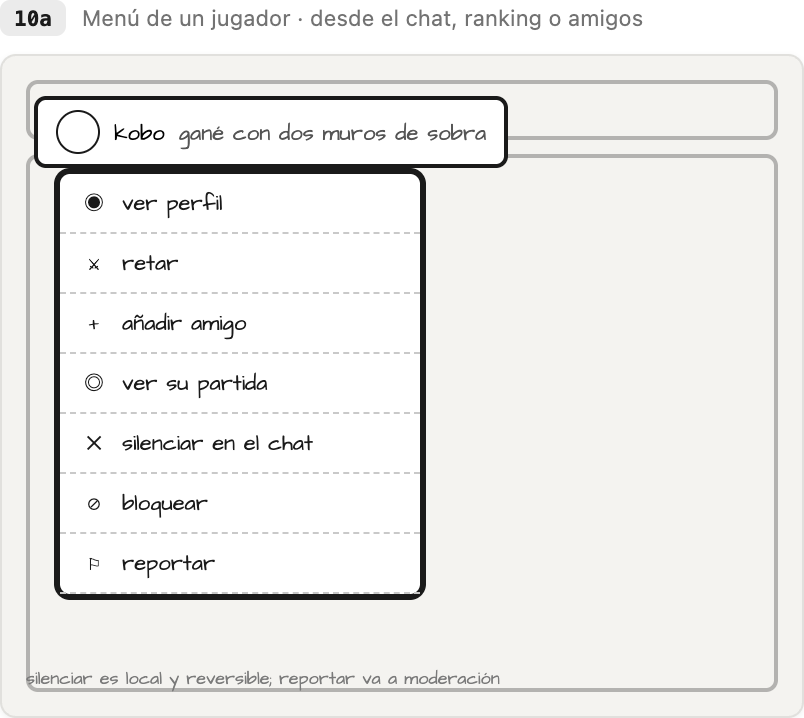
\includegraphics[width=\linewidth]{Prototipos/10a}\par\smallskip
{\footnotesize\textit{Prototipo 10a: Menú de un jugador}}
\end{minipage}
\par\medskip
\end{center}

%--- F-40 Responder o cancelar una solicitud de amistad
\begin{prototipocrud}{F-40}{Responder o cancelar una solicitud de amistad}
  \crudFila{Operación}{Creación (C), Eliminación (D)}
  \crudFila{Caso de uso}{\mbox{CU-31}}
  \crudFila{Actor}{Jugador con cuenta registrada}
  \crudFila{Prototipos}{5c, Solicitudes · entrantes y enviadas.}
  \crudFila{Datos de entrada}{\begin{crudlista}
    \item \texttt{id\_\allowbreak{}solicitud}.
    \item Acción: aceptar o rechazar, si es destinatario; cancelar, si es solicitante.
    \item Token de sesión.
  \end{crudlista}}
  \crudFila{Datos que se consultan}{\begin{crudlista}
    \item \textit{Solicitud}: que el usuario sea su destinatario o su solicitante.
    \item \textit{Amistad}: cuántos amigos tiene cada uno.
    \item \textit{Bloqueo}: si surgió uno desde que se envió.
  \end{crudlista}}
  \crudFila{Datos que se crean}{\begin{crudlista}
    \item \textit{Amistad}: \texttt{id\_\allowbreak{}usuario\_\allowbreak{}a} con el identificador menor, \texttt{id\_\allowbreak{}usuario\_\allowbreak{}b} con el mayor y \texttt{fecha\_\allowbreak{}amistad}, solo si acepta.
  \end{crudlista}}
  \crudFila{Datos que se modifican}{Ninguno.}
  \crudFila{Datos que se eliminan}{\begin{crudlista}
    \item \textit{Solicitud}: se elimina al aceptar, rechazar o cancelar. Borrado físico.
  \end{crudlista}}
  \crudFila{Reglas de negocio}{\begin{crudlista}
    \item Solo el destinatario acepta o rechaza, y solo el solicitante cancela (\mbox{CU-31} \mbox{RN-01}).
    \item El límite de cien amigos se vuelve a comprobar al aceptar (\mbox{CU-31} \mbox{RN-02}).
    \item Cada amistad se guarda una sola vez por par ordenado, con una restricción en la tabla (\mbox{CU-31} \mbox{RN-03}).
    \item Rechazar no notifica al solicitante (\mbox{CU-31} \mbox{RN-04}).
    \item Una solicitud sin responder caduca a los treinta días (\mbox{CU-31} \mbox{RN-05}).
  \end{crudlista}}
  \crudFila{Resultado esperado}{Si se aceptó, ambos jugadores se ven en su lista de amigos; en cualquier caso, la solicitud desaparece.}
\end{prototipocrud}
\par\nopagebreak\smallskip
\begin{center}
\begin{minipage}[t]{0.50\textwidth}\centering
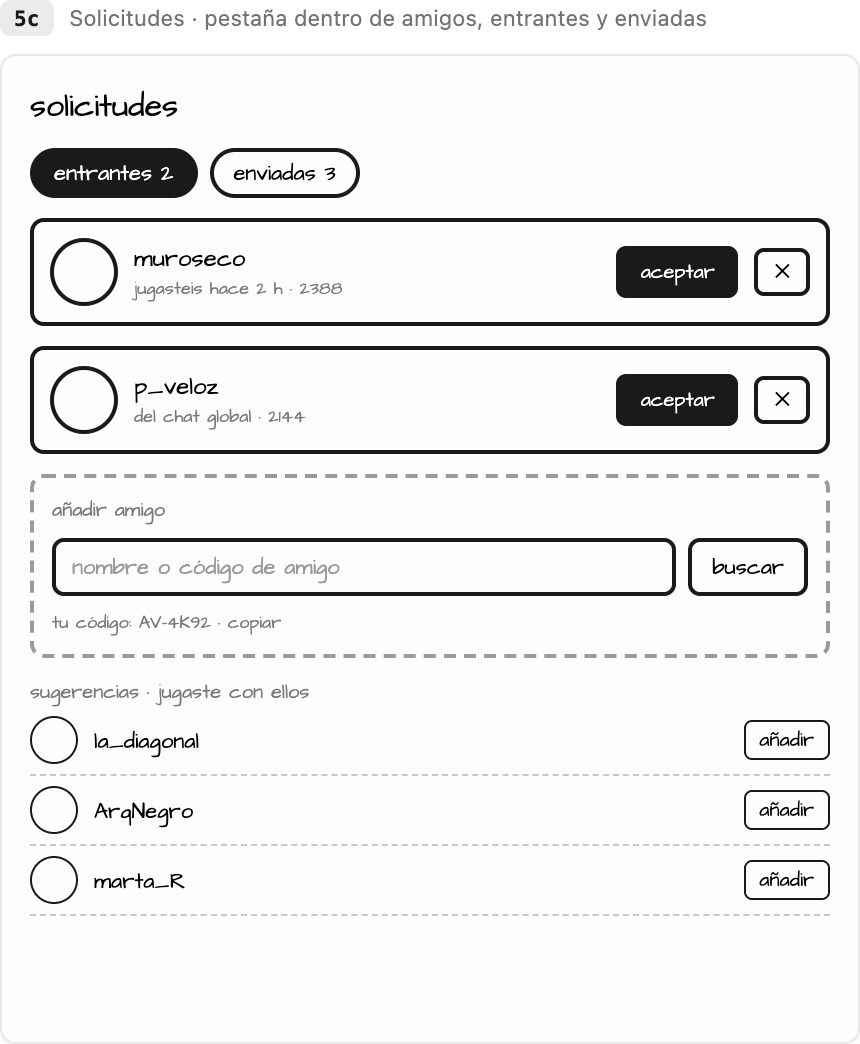
\includegraphics[width=\linewidth]{Prototipos/5c}\par\smallskip
{\footnotesize\textit{Prototipo 5c: Solicitudes · entrantes y enviadas}}
\end{minipage}
\par\medskip
\end{center}

%--- F-41 Consultar lista de amigos
\begin{prototipocrud}{F-41}{Consultar lista de amigos}
  \crudFila{Operación}{Consulta (R)}
  \crudFila{Caso de uso}{\mbox{CU-30}, \mbox{CU-31}}
  \crudFila{Actor}{Jugador con cuenta registrada}
  \crudFila{Prototipos}{2b, Amigos · pantalla completa con pestañas; 13a, Desde amigos · quién está jugando.}
  \crudFila{Datos de entrada}{\begin{crudlista}
    \item Token de sesión.
  \end{crudlista}}
  \crudFila{Datos que se consultan}{\begin{crudlista}
    \item \textit{Amistad}: las del usuario, en cualquiera de las dos columnas.
    \item \textit{Usuario}: \texttt{nickname}, \texttt{id\_\allowbreak{}icono}, \texttt{estado\_\allowbreak{}cuenta} de cada amigo.
    \item \textit{Sesion}: si el amigo tiene alguna abierta, para su estado de conexión.
    \item \textit{Participacion} y \textit{Partida}: si el amigo está jugando y si la partida admite espectadores.
    \item \textit{Solicitud}: entrantes y enviadas.
  \end{crudlista}}
  \crudFila{Datos que se crean}{Ninguno.}
  \crudFila{Datos que se modifican}{Ninguno.}
  \crudFila{Datos que se eliminan}{Ninguno.}
  \crudFila{Reglas de negocio}{\begin{crudlista}
    \item Un amigo está jugando si tiene una participación sin terminar (\mbox{D-11}).
    \item Las cuentas \texttt{ELIMINADA} no aparecen en la lista.
  \end{crudlista}}
  \crudFila{Resultado esperado}{Lista de amigos con su estado, un bloque de quién está jugando ahora con acceso a ver su partida, y las solicitudes pendientes.}
\end{prototipocrud}
\par\nopagebreak\smallskip
\begin{center}
\begin{minipage}[t]{0.48\textwidth}\centering
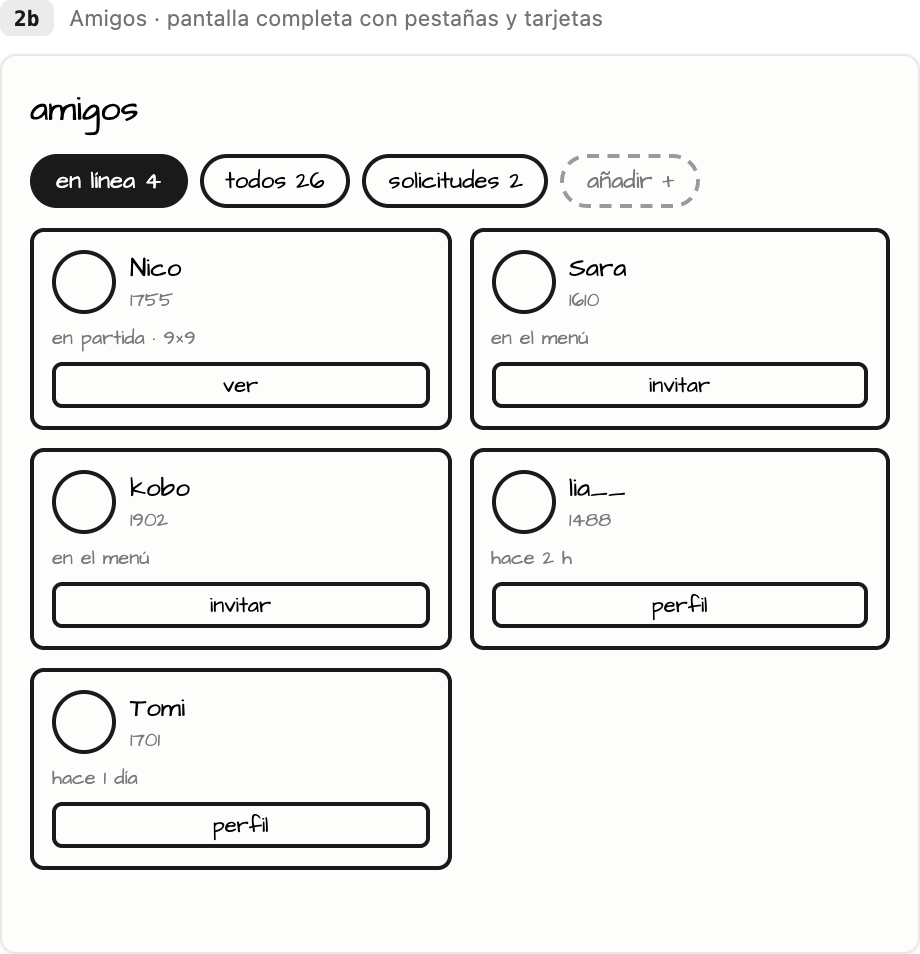
\includegraphics[width=\linewidth]{Prototipos/2b}\par\smallskip
{\footnotesize\textit{Prototipo 2b: Amigos · pantalla completa con pestañas}}
\end{minipage}\hfill
\begin{minipage}[t]{0.48\textwidth}\centering
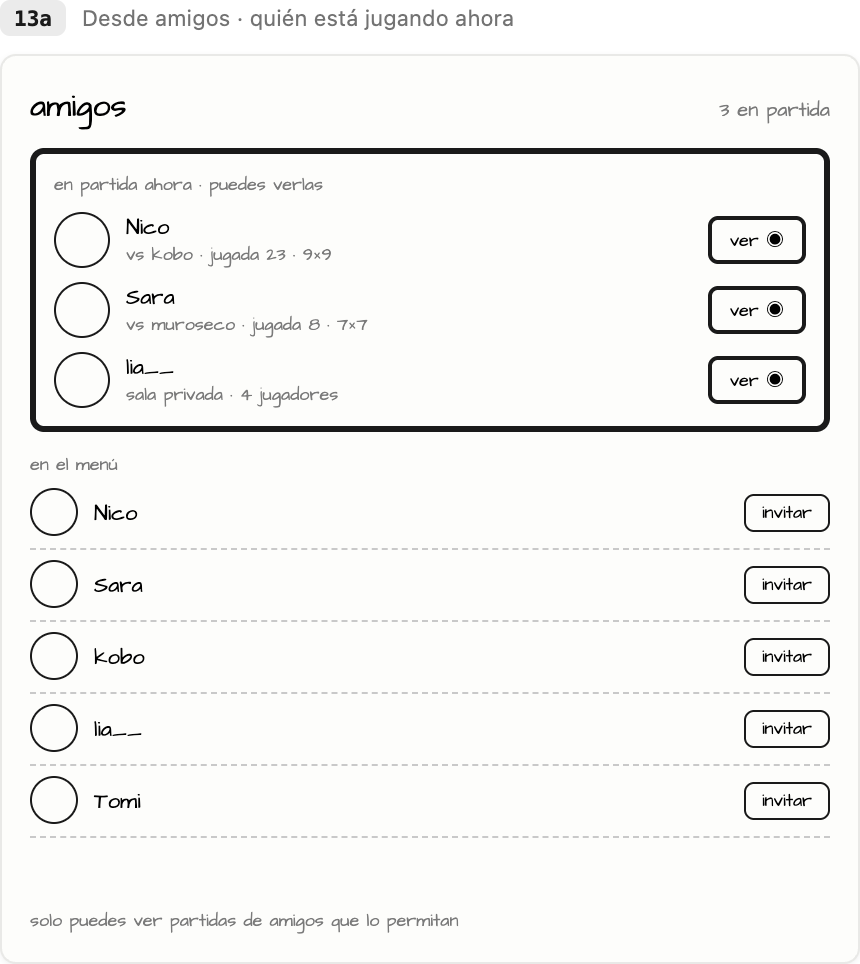
\includegraphics[width=\linewidth]{Prototipos/13a}\par\smallskip
{\footnotesize\textit{Prototipo 13a: Desde amigos · quién está jugando}}
\end{minipage}
\par\medskip
\end{center}

%--- F-42 Eliminar a un amigo
\begin{prototipocrud}{F-42}{Eliminar a un amigo}
  \crudFila{Operación}{Eliminación (D)}
  \crudFila{Caso de uso}{\mbox{CU-49}}
  \crudFila{Actor}{Jugador con cuenta registrada}
  \crudFila{Prototipos}{Sin prototipo. El menú de un jugador (10a, \mbox{F-39}) no incluye la opción de eliminar amigo.}
  \crudFila{Datos de entrada}{\begin{crudlista}
    \item \texttt{id\_\allowbreak{}usuario} del amigo.
    \item Confirmación.
    \item Token de sesión.
  \end{crudlista}}
  \crudFila{Datos que se consultan}{\begin{crudlista}
    \item \textit{Amistad}: la del par ordenado.
  \end{crudlista}}
  \crudFila{Datos que se crean}{Ninguno.}
  \crudFila{Datos que se modifican}{Ninguno.}
  \crudFila{Datos que se eliminan}{\begin{crudlista}
    \item \textit{Amistad}: la fila del par. Borrado físico.
  \end{crudlista}}
  \crudFila{Reglas de negocio}{\begin{crudlista}
    \item La eliminación es recíproca (\mbox{CU-49} \mbox{RN-01}).
    \item No se notifica al otro jugador (\mbox{CU-49} \mbox{RN-03}).
    \item No afecta a salas, partidas ni invitaciones en curso (\mbox{CU-49} \mbox{RN-04}).
    \item No bloquea: pueden volver a enviarse solicitud (\mbox{CU-49} \mbox{RN-05}).
  \end{crudlista}}
  \crudFila{Resultado esperado}{Ninguno de los dos ve al otro en su lista de amigos, y su historial de partidas juntos se conserva.}
\end{prototipocrud}

%--- F-43 Silenciar, bloquear y deshacerlo
\begin{prototipocrud}{F-43}{Silenciar, bloquear y deshacerlo}
  \crudFila{Operación}{Creación (C), Eliminación (D)}
  \crudFila{Caso de uso}{\mbox{CU-33}}
  \crudFila{Actor}{Jugador}
  \crudFila{Prototipos}{10c, Silenciados y bloqueados. También 10a, las opciones ``silenciar'' y ``bloquear'' (\mbox{F-39}).}
  \crudFila{Datos de entrada}{\begin{crudlista}
    \item \texttt{id\_\allowbreak{}usuario} del otro jugador.
    \item Acción: silenciar, dejar de silenciar, bloquear o desbloquear.
    \item Token de sesión.
  \end{crudlista}}
  \crudFila{Datos que se consultan}{\begin{crudlista}
    \item \textit{Silencio} y \textit{Bloqueo}: si ya existen.
    \item \textit{Amistad}, \textit{Solicitud} e \textit{Invitacion}: entre ambos.
    \item \textit{ColaEmparejamiento} y \textit{SalaParticipante}: si coinciden.
  \end{crudlista}}
  \crudFila{Datos que se crean}{\begin{crudlista}
    \item \textit{Silencio}: \texttt{id\_\allowbreak{}usuario}, \texttt{id\_\allowbreak{}silenciado}, \texttt{fecha\_\allowbreak{}silencio}.
    \item \textit{Bloqueo}: \texttt{id\_\allowbreak{}bloqueador}, \texttt{id\_\allowbreak{}bloqueado}, \texttt{fecha\_\allowbreak{}bloqueo}.
  \end{crudlista}}
  \crudFila{Datos que se modifican}{\begin{crudlista}
    \item \textit{Invitacion}: las pendientes entre ambos pasan a \texttt{EXPIRADA}, al bloquear.
  \end{crudlista}}
  \crudFila{Datos que se eliminan}{\begin{crudlista}
    \item Al bloquear: la \textit{Amistad}, las \textit{Solicitud} pendientes entre ambos y, si comparten sala, la \textit{SalaParticipante} del que debe salir. Borrado físico.
    \item Al dejar de silenciar o desbloquear: la fila de \textit{Silencio} o de \textit{Bloqueo}. Borrado físico.
  \end{crudlista}}
  \crudFila{Reglas de negocio}{\begin{crudlista}
    \item Silenciar oculta mensajes y emotes, es reversible y no pide confirmación (\mbox{CU-33} \mbox{RN-01}).
    \item Ni el silencio ni el bloqueo se notifican (\mbox{CU-33} \mbox{RN-02}).
    \item Un bloqueo no interrumpe una partida en curso (\mbox{CU-33} \mbox{RN-04}).
    \item Desbloquear no restaura la amistad eliminada (\mbox{CU-33} \mbox{RN-06}).
    \item El bloqueo no afecta a la moderación (\mbox{CU-33} \mbox{RN-07}).
    \item Los invitados pueden silenciar, pero no bloquear.
  \end{crudlista}}
  \crudFila{Resultado esperado}{Queda aplicado o retirado el silencio o el bloqueo, con efecto inmediato en el chat, las salas y el emparejamiento.}
\end{prototipocrud}
\par\nopagebreak\smallskip
\begin{center}
\begin{minipage}[t]{0.50\textwidth}\centering
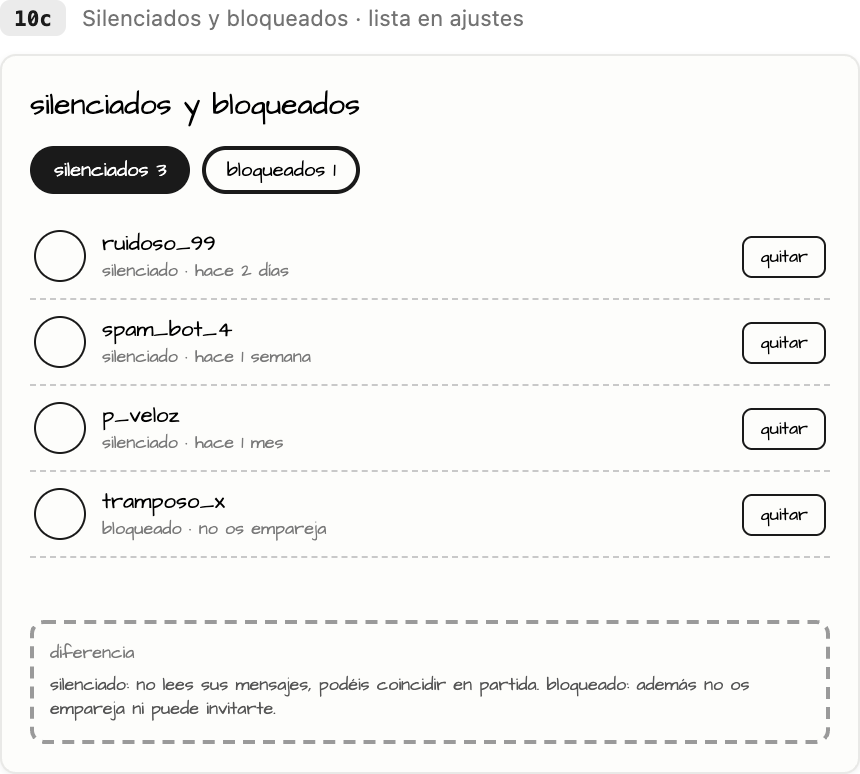
\includegraphics[width=\linewidth]{Prototipos/10c}\par\smallskip
{\footnotesize\textit{Prototipo 10c: Silenciados y bloqueados}}
\end{minipage}
\par\medskip
\end{center}

%--- F-44 Enviar mensaje de chat
\begin{prototipocrud}{F-44}{Enviar mensaje de chat}
  \crudFila{Operación}{Creación (C)}
  \crudFila{Caso de uso}{\mbox{CU-28}}
  \crudFila{Actor}{Jugador o espectador con sesión}
  \crudFila{Prototipos}{20c, Chat desplegado desde el icono.}
  \crudFila{Datos de entrada}{\begin{crudlista}
    \item \texttt{canal}: \texttt{PARTIDA}, \texttt{GLOBAL}, \texttt{AMIGOS}, \texttt{SALA} o \texttt{ESPECTADORES}.
    \item \texttt{texto}: hasta el largo máximo, no vacío.
    \item Token de sesión.
  \end{crudlista}}
  \crudFila{Datos que se consultan}{\begin{crudlista}
    \item \textit{Sancion}: activas con \texttt{ambito} = \texttt{CHAT}.
    \item \textit{Participacion}, \textit{Amistad} o \textit{SalaParticipante}: acceso al canal.
    \item \textit{PalabraProhibida}: con \texttt{ambito} de chat.
    \item \textit{Mensaje}: los recientes del autor, para el ritmo de envío.
    \item \textit{Bloqueo} y \textit{Silencio}: para decidir a quién se entrega.
  \end{crudlista}}
  \crudFila{Datos que se crean}{\begin{crudlista}
    \item \textit{Mensaje}: \texttt{canal}, \texttt{id\_\allowbreak{}autor}, \texttt{texto}, \texttt{fecha\_\allowbreak{}envio}, e \texttt{id\_\allowbreak{}partida} o \texttt{id\_\allowbreak{}sala} según el canal.
  \end{crudlista}}
  \crudFila{Datos que se modifican}{Ninguno.}
  \crudFila{Datos que se eliminan}{Ninguno.}
  \crudFila{Reglas de negocio}{\begin{crudlista}
    \item Todo mensaje se filtra en el servidor y el rechazo no dice qué término saltó (\mbox{CU-28} \mbox{RN-01}, \mbox{RN-02}).
    \item El ritmo de envío está acotado por canal (\mbox{CU-28} \mbox{RN-04}).
    \item Una sanción de chat impide escribir pero no leer ni jugar (\mbox{CU-28} \mbox{RN-05}, \mbox{D-05}).
    \item Si el filtro no puede aplicarse, el mensaje se rechaza (\mbox{CU-28} \mbox{RN-11}).
    \item Un mensaje rechazado no se guarda.
    \item Los emotes no son mensajes y no se guardan (\mbox{CU-29}, \mbox{D-10}).
  \end{crudlista}}
  \crudFila{Resultado esperado}{El mensaje queda guardado y llega a los destinatarios del canal que no hayan bloqueado ni silenciado al autor.}
\end{prototipocrud}
\par\nopagebreak\smallskip
\begin{center}
\begin{minipage}[t]{0.50\textwidth}\centering
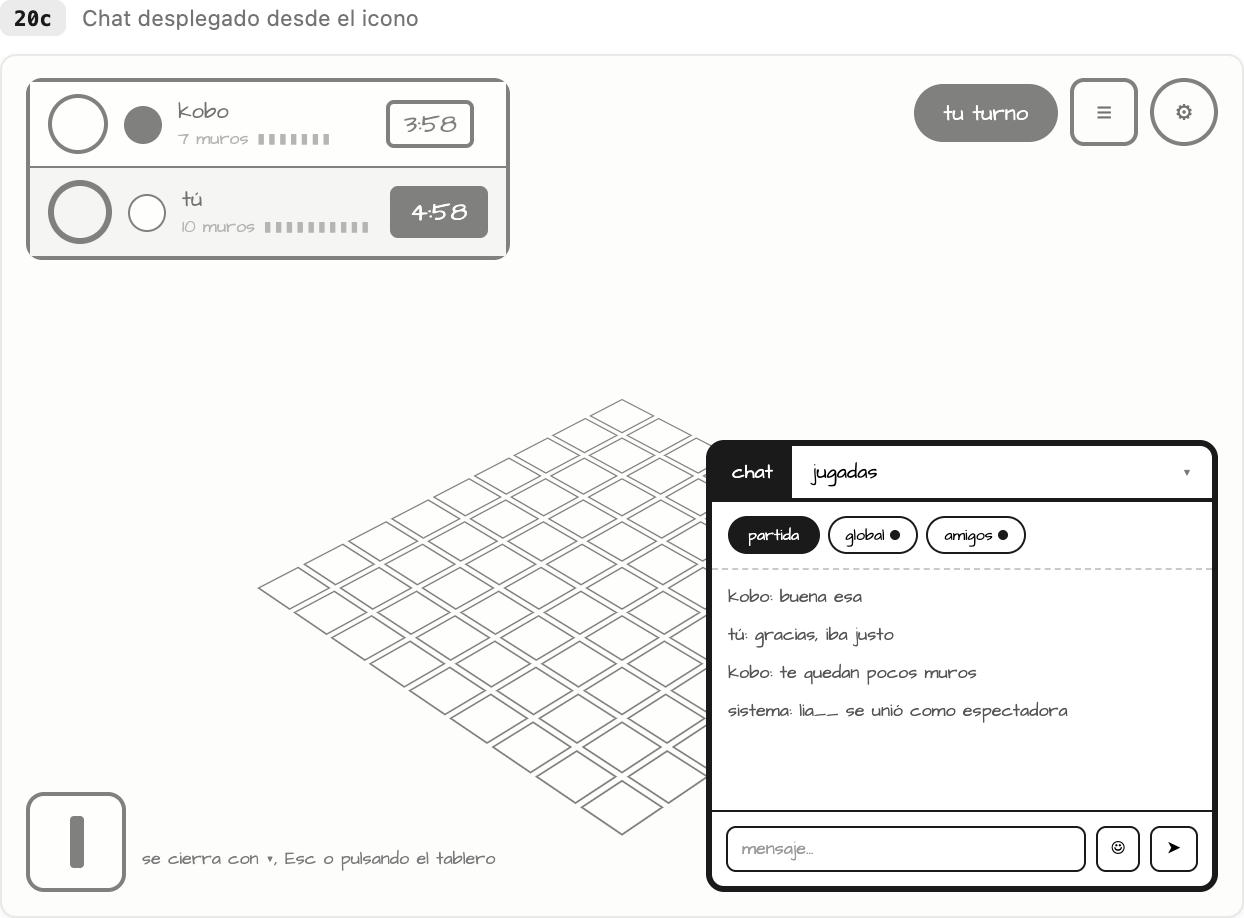
\includegraphics[width=\linewidth]{Prototipos/20c}\par\smallskip
{\footnotesize\textit{Prototipo 20c: Chat desplegado desde el icono}}
\end{minipage}
\par\medskip
\end{center}

%--- F-45 Consultar mensajes de un canal
\begin{prototipocrud}{F-45}{Consultar mensajes de un canal}
  \crudFila{Operación}{Consulta (R)}
  \crudFila{Caso de uso}{\mbox{CU-28}}
  \crudFila{Actor}{Jugador, invitado o espectador}
  \crudFila{Prototipos}{5f, Chat global expandido.}
  \crudFila{Datos de entrada}{\begin{crudlista}
    \item \texttt{canal} y, si aplica, \texttt{id\_\allowbreak{}partida} o \texttt{id\_\allowbreak{}sala}.
    \item Último mensaje ya leído.
    \item Token de sesión, si lo hay.
  \end{crudlista}}
  \crudFila{Datos que se consultan}{\begin{crudlista}
    \item \textit{Mensaje}: los del canal posteriores al último leído.
    \item \textit{Usuario}: \texttt{nickname} de cada autor.
    \item \textit{Bloqueo} y \textit{Silencio}: para ocultar a quien corresponda.
  \end{crudlista}}
  \crudFila{Datos que se crean}{Ninguno.}
  \crudFila{Datos que se modifican}{Ninguno.}
  \crudFila{Datos que se eliminan}{Ninguno.}
  \crudFila{Reglas de negocio}{\begin{crudlista}
    \item Los mensajes no se traducen (\mbox{CU-28} \mbox{RN-12}).
    \item Los mensajes de un jugador bloqueado o silenciado no se muestran a quien lo bloqueó o silenció.
    \item El chat de espectadores está separado del de los jugadores (\mbox{CU-28} \mbox{RN-09}).
  \end{crudlista}}
  \crudFila{Resultado esperado}{Los mensajes del canal, con indicador de nuevos.}
\end{prototipocrud}
\par\nopagebreak\smallskip
\begin{center}
\begin{minipage}[t]{0.50\textwidth}\centering
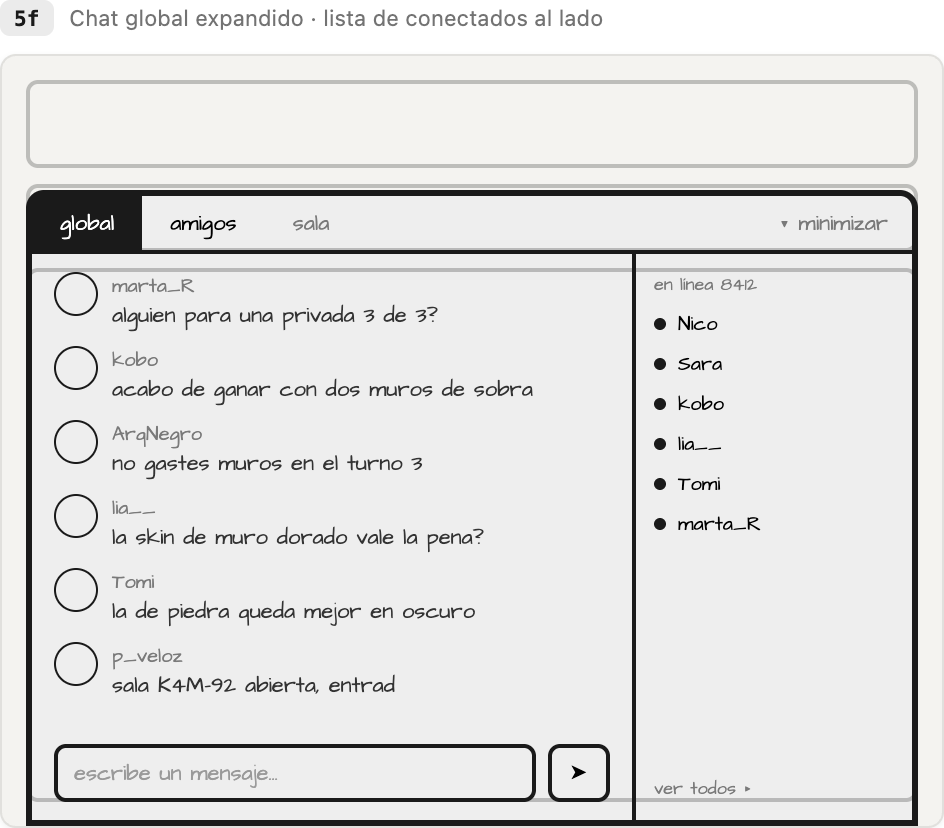
\includegraphics[width=\linewidth]{Prototipos/5f}\par\smallskip
{\footnotesize\textit{Prototipo 5f: Chat global expandido}}
\end{minipage}
\par\medskip
\end{center}

\subsection*{Moderación y administración}
\addcontentsline{toc}{subsection}{Moderación y administración}

Nada de lo que produce la moderación se elimina: reportes, sanciones y apelaciones son evidencia, y una sanción retirada debe seguir siendo consultable para poder revisarse. Todas las acciones quedan en la bitácora de moderación, incluida la consulta de las propias bitácoras.

%--- F-46 Reportar a un jugador
\begin{prototipocrud}{F-46}{Reportar a un jugador}
  \crudFila{Operación}{Creación (C)}
  \crudFila{Caso de uso}{\mbox{CU-42}}
  \crudFila{Actor}{Jugador con cuenta registrada}
  \crudFila{Prototipos}{10b, Reportar · motivo y pruebas.}
  \crudFila{Datos de entrada}{\begin{crudlista}
    \item \texttt{id\_\allowbreak{}reportado}.
    \item \texttt{id\_\allowbreak{}motivo}: uno de los cinco del catálogo.
    \item \texttt{descripcion}: texto opcional hasta el largo máximo.
    \item \texttt{id\_\allowbreak{}partida}, si se reporta desde una partida.
    \item Token de sesión.
  \end{crudlista}}
  \crudFila{Datos que se consultan}{\begin{crudlista}
    \item \textit{Usuario}: el reportado y su \texttt{estado\_\allowbreak{}cuenta}.
    \item \textit{MotivoReporte}: el catálogo.
    \item \textit{Reporte}: duplicados y número de reportes recientes del denunciante.
  \end{crudlista}}
  \crudFila{Datos que se crean}{\begin{crudlista}
    \item \textit{Reporte}: \texttt{id\_\allowbreak{}denunciante}, \texttt{id\_\allowbreak{}reportado}, \texttt{id\_\allowbreak{}motivo}, \texttt{descripcion}, \texttt{id\_\allowbreak{}partida}, \texttt{fecha\_\allowbreak{}reporte}, \texttt{estado} = \texttt{PENDIENTE}.
  \end{crudlista}}
  \crudFila{Datos que se modifican}{Ninguno.}
  \crudFila{Datos que se eliminan}{Ninguno.}
  \crudFila{Reglas de negocio}{\begin{crudlista}
    \item Las pruebas se adjuntan por referencia a la partida, no por copia (\mbox{CU-42} \mbox{RN-01}).
    \item No se reporta dos veces al mismo jugador por la misma partida (\mbox{CU-42} \mbox{RN-03}).
    \item Reportar no sanciona (\mbox{CU-42} \mbox{RN-04}).
    \item El número de reportes por periodo está acotado (\mbox{CU-42} \mbox{RN-06}).
    \item Los invitados no reportan (\mbox{CU-42} \mbox{RN-07}).
  \end{crudlista}}
  \crudFila{Resultado esperado}{Existe un reporte pendiente de revisión con acceso a la repetición y al chat de la partida.}
\end{prototipocrud}
\par\nopagebreak\smallskip
\begin{center}
\begin{minipage}[t]{0.50\textwidth}\centering
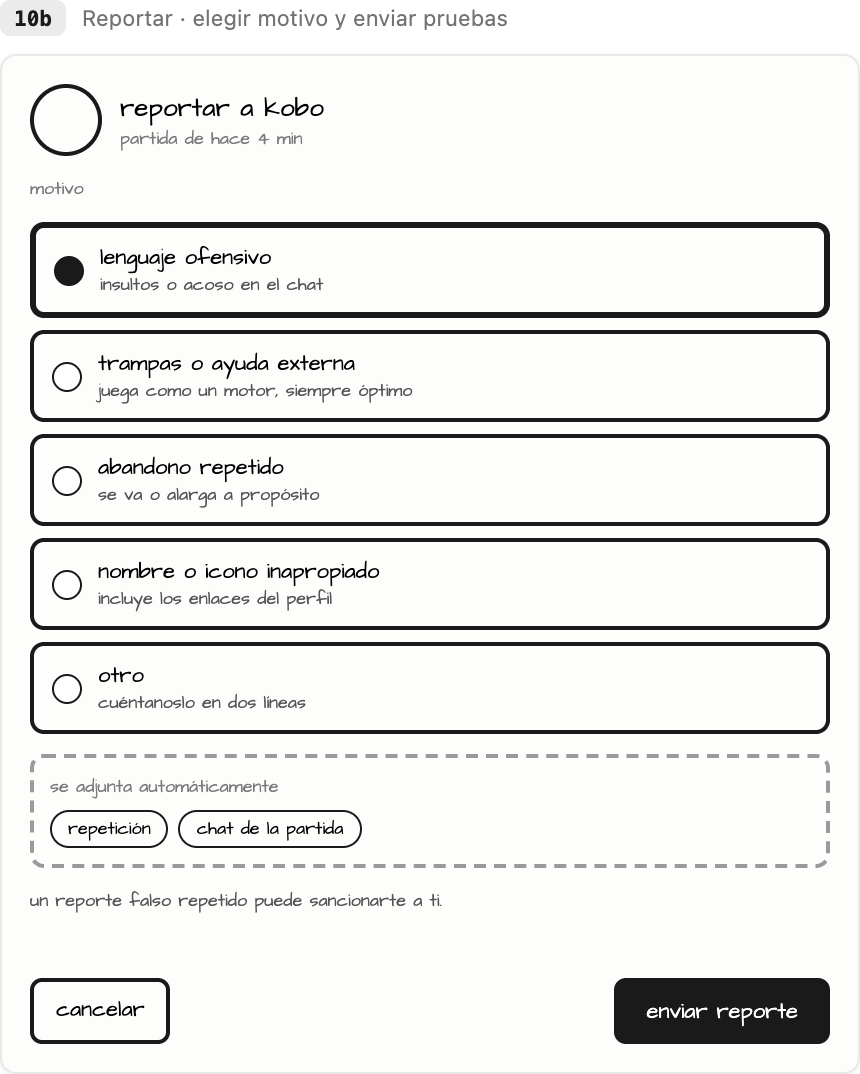
\includegraphics[width=\linewidth]{Prototipos/10b}\par\smallskip
{\footnotesize\textit{Prototipo 10b: Reportar · motivo y pruebas}}
\end{minipage}
\par\medskip
\end{center}

%--- F-47 Revisar y resolver un reporte
\begin{prototipocrud}{F-47}{Revisar y resolver un reporte}
  \crudFila{Operación}{Actualización (U)}
  \crudFila{Caso de uso}{\mbox{CU-43}}
  \crudFila{Actor}{Moderador}
  \crudFila{Prototipos}{Sin prototipo: no hay pantallas de moderación.}
  \crudFila{Datos de entrada}{\begin{crudlista}
    \item \texttt{id\_\allowbreak{}reporte}.
    \item Acción: tomar, liberar o resolver.
    \item Resolución: sin sanción o con sanción.
    \item \texttt{nota\_\allowbreak{}resolucion}: obligatoria.
    \item Token de sesión.
  \end{crudlista}}
  \crudFila{Datos que se consultan}{\begin{crudlista}
    \item \textit{Usuario}: \texttt{rol} del moderador.
    \item \textit{Reporte}: los pendientes con su \textit{MotivoReporte}; los que llevan más de treinta minutos en revisión.
    \item \textit{Partida}, \textit{Jugada} y \textit{Mensaje}: las pruebas.
    \item \textit{Sancion}: el historial del reportado.
  \end{crudlista}}
  \crudFila{Datos que se crean}{\begin{crudlista}
    \item \textit{BitacoraModeracion}: la toma, la liberación y la resolución.
  \end{crudlista}}
  \crudFila{Datos que se modifican}{\begin{crudlista}
    \item \textit{Reporte}: \texttt{estado} (\texttt{EN\_\allowbreak{}REVISION}, \texttt{PENDIENTE}, \texttt{RESUELTO\_\allowbreak{}SIN\_\allowbreak{}SANCION}), \texttt{id\_\allowbreak{}moderador}, \texttt{fecha\_\allowbreak{}asignacion}, \texttt{nota\_\allowbreak{}resolucion}, \texttt{fecha\_\allowbreak{}resolucion}.
  \end{crudlista}}
  \crudFila{Datos que se eliminan}{Ninguno.}
  \crudFila{Reglas de negocio}{\begin{crudlista}
    \item Solo un usuario con \texttt{rol} = \texttt{MODERADOR}, comprobado en cada solicitud (\mbox{CU-43} \mbox{RN-01}).
    \item Un reporte en revisión lo atiende un solo moderador (\mbox{CU-43} \mbox{RN-02}).
    \item A los treinta minutos sin resolver vuelve a la cola (\mbox{CU-43} \mbox{RN-03}).
    \item Un moderador no revisa reportes en los que es parte (\mbox{CU-43} \mbox{RN-04}).
    \item El resultado no se comunica al denunciante (\mbox{CU-43} \mbox{RN-05}).
    \item Si se resuelve con sanción, continúa en la aplicación de la sanción.
  \end{crudlista}}
  \crudFila{Resultado esperado}{El reporte queda resuelto, con el moderador que lo atendió y su nota, o vuelve a la cola si se libera.}
\end{prototipocrud}

%--- F-48 Aplicar una sanción
\begin{prototipocrud}{F-48}{Aplicar una sanción}
  \crudFila{Operación}{Creación (C), Actualización (U)}
  \crudFila{Caso de uso}{\mbox{CU-44}}
  \crudFila{Actor}{Moderador}
  \crudFila{Prototipos}{10d, Te sancionan · chat restringido. Muestra el efecto sobre el jugador; la pantalla del moderador no está prototipada.}
  \crudFila{Datos de entrada}{\begin{crudlista}
    \item \texttt{id\_\allowbreak{}usuario} sancionado.
    \item \texttt{ambito}: \texttt{CUENTA} o \texttt{CHAT}.
    \item \texttt{tipo}: \texttt{TEMPORAL} o \texttt{PERMANENTE}.
    \item Duración, si es temporal.
    \item \texttt{motivo}: texto obligatorio.
    \item \texttt{id\_\allowbreak{}reporte}, opcional.
    \item Token de sesión.
  \end{crudlista}}
  \crudFila{Datos que se consultan}{\begin{crudlista}
    \item \textit{Usuario}: \texttt{rol} del moderador y del sancionado, \texttt{estado\_\allowbreak{}cuenta}.
    \item \textit{Sancion}: activas del mismo ámbito.
    \item \textit{Sesion} y \textit{Participacion} del sancionado.
  \end{crudlista}}
  \crudFila{Datos que se crean}{\begin{crudlista}
    \item \textit{Sancion}: \texttt{id\_\allowbreak{}usuario}, \texttt{id\_\allowbreak{}moderador}, \texttt{ambito}, \texttt{tipo}, \texttt{motivo}, \texttt{fecha\_\allowbreak{}inicio}, \texttt{fecha\_\allowbreak{}fin}, \texttt{activa} = 1, \texttt{id\_\allowbreak{}reporte}.
    \item \textit{BitacoraModeracion}.
  \end{crudlista}}
  \crudFila{Datos que se modifican}{\begin{crudlista}
    \item \textit{Usuario}: \texttt{estado\_\allowbreak{}cuenta} = \texttt{SUSPENDIDA} o \texttt{BANEADA}, solo con ámbito de cuenta.
    \item \textit{Sesion}: \texttt{fecha\_\allowbreak{}fin} y \texttt{motivo\_\allowbreak{}cierre} = \texttt{SANCION}, solo con ámbito de cuenta.
    \item \textit{Participacion} sin terminar: se cierra por \texttt{ABANDONO}, solo con ámbito de cuenta.
    \item \textit{Reporte}: \texttt{estado} = \texttt{RESUELTO\_\allowbreak{}CON\_\allowbreak{}SANCION}.
    \item \textit{Sancion} anterior del mismo ámbito, si se sustituye: \texttt{activa} = 0, \texttt{fecha\_\allowbreak{}retiro}, \texttt{id\_\allowbreak{}sancion\_\allowbreak{}sustituta}.
  \end{crudlista}}
  \crudFila{Datos que se eliminan}{Ninguno.}
  \crudFila{Reglas de negocio}{\begin{crudlista}
    \item Un moderador no sanciona a otro moderador ni a un administrador (\mbox{CU-44} \mbox{RN-02}).
    \item La sanción de chat no toca la cuenta, las sesiones ni las partidas (\mbox{CU-44} \mbox{RN-03}, \mbox{D-05}).
    \item Una sanción permanente tiene \texttt{fecha\_\allowbreak{}fin} nula (\mbox{CU-44} \mbox{RN-04}).
    \item Toda sanción lleva motivo escrito y autor registrado (\mbox{CU-44} \mbox{RN-06}, \mbox{RN-07}).
    \item No se acumulan dos sanciones activas del mismo ámbito (\mbox{CU-44} \mbox{RN-09}).
  \end{crudlista}}
  \crudFila{Resultado esperado}{La sanción surte efecto de inmediato y queda registrada con su autor, su motivo y su vigencia.}
\end{prototipocrud}
\par\nopagebreak\smallskip
\begin{center}
\begin{minipage}[t]{0.50\textwidth}\centering
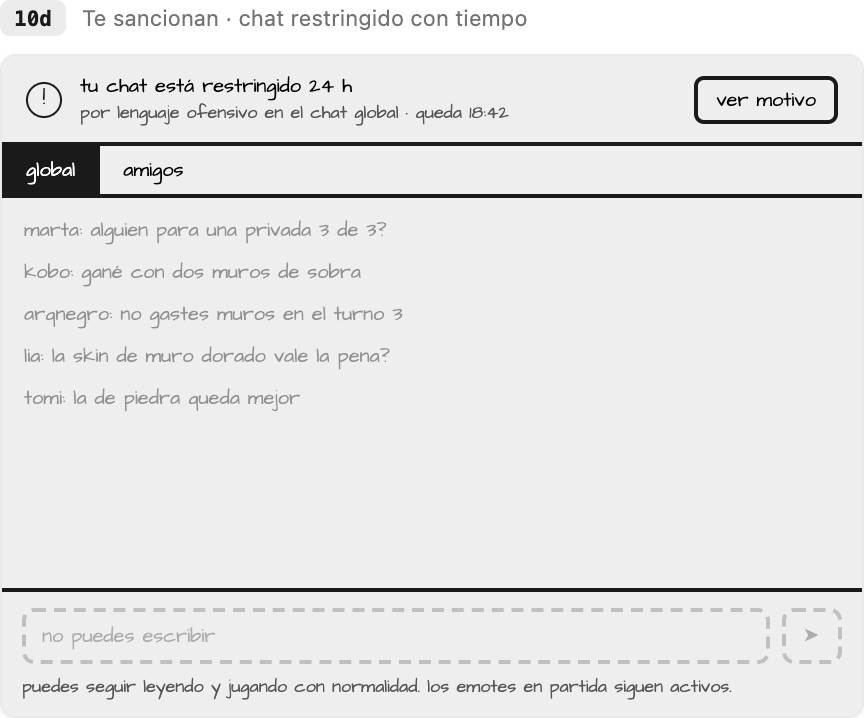
\includegraphics[width=\linewidth]{Prototipos/10d}\par\smallskip
{\footnotesize\textit{Prototipo 10d: Te sancionan · chat restringido}}
\end{minipage}
\par\medskip
\end{center}

%--- F-49 Apelar una sanción
\begin{prototipocrud}{F-49}{Apelar una sanción}
  \crudFila{Operación}{Creación (C)}
  \crudFila{Caso de uso}{\mbox{CU-45}}
  \crudFila{Actor}{Jugador sancionado}
  \crudFila{Prototipos}{10e, Aviso de sanción · detalle y apelación.}
  \crudFila{Datos de entrada}{\begin{crudlista}
    \item \texttt{id\_\allowbreak{}sancion}.
    \item \texttt{texto} de la apelación, hasta el largo máximo.
    \item Token de sesión, o el token de apelación emitido por el inicio de sesión.
  \end{crudlista}}
  \crudFila{Datos que se consultan}{\begin{crudlista}
    \item \textit{Sancion}: que sea propia y esté activa.
    \item \textit{Apelacion}: si ya existe una para esa sanción.
    \item \textit{PalabraProhibida}: para marcar el texto.
  \end{crudlista}}
  \crudFila{Datos que se crean}{\begin{crudlista}
    \item \textit{Apelacion}: \texttt{id\_\allowbreak{}sancion}, \texttt{texto}, \texttt{marca\_\allowbreak{}lenguaje}, \texttt{fecha\_\allowbreak{}apelacion}, \texttt{estado} = \texttt{PENDIENTE}.
  \end{crudlista}}
  \crudFila{Datos que se modifican}{Ninguno.}
  \crudFila{Datos que se eliminan}{Ninguno.}
  \crudFila{Reglas de negocio}{\begin{crudlista}
    \item Una sola apelación por sanción, y solo de sanciones activas (\mbox{CU-45} \mbox{RN-01}, \mbox{RN-02}).
    \item Apelar no suspende la sanción (\mbox{CU-45} \mbox{RN-03}).
    \item El texto no se rechaza por lenguaje: se marca para el moderador (\mbox{CU-45} \mbox{RN-04}).
    \item Una sanción de cuenta se apela sin iniciar sesión, con un token de corta vigencia (\mbox{CU-45} \mbox{RN-05}).
  \end{crudlista}}
  \crudFila{Resultado esperado}{La apelación queda pendiente en la cola de moderación.}
\end{prototipocrud}
\par\nopagebreak\smallskip
\begin{center}
\begin{minipage}[t]{0.50\textwidth}\centering
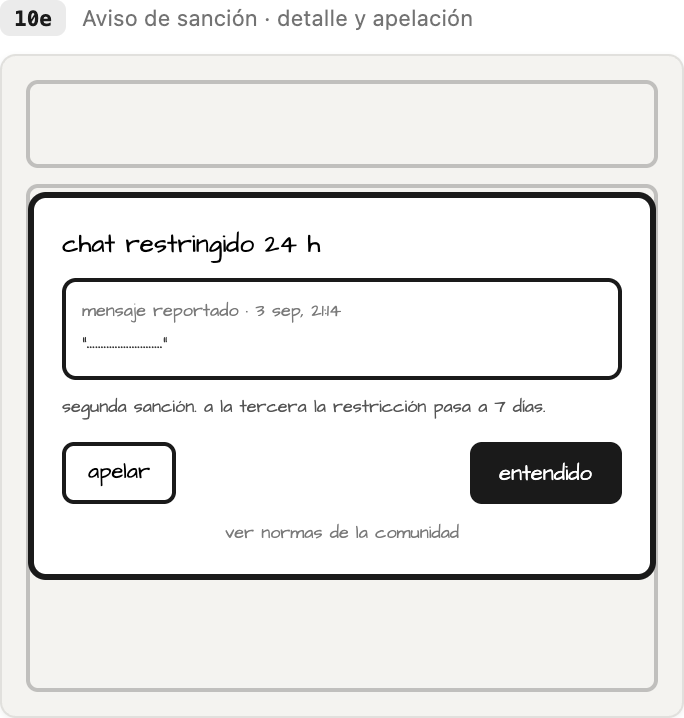
\includegraphics[width=\linewidth]{Prototipos/10e}\par\smallskip
{\footnotesize\textit{Prototipo 10e: Aviso de sanción · detalle y apelación}}
\end{minipage}
\par\medskip
\end{center}

%--- F-50 Resolver una apelación
\begin{prototipocrud}{F-50}{Resolver una apelación}
  \crudFila{Operación}{Actualización (U)}
  \crudFila{Caso de uso}{\mbox{CU-43} (\mbox{FA-08})}
  \crudFila{Actor}{Moderador}
  \crudFila{Prototipos}{Sin prototipo: no hay pantallas de moderación.}
  \crudFila{Datos de entrada}{\begin{crudlista}
    \item \texttt{id\_\allowbreak{}apelacion}.
    \item Decisión: mantener o retirar la sanción.
    \item \texttt{nota\_\allowbreak{}resolucion}: obligatoria.
    \item Token de sesión.
  \end{crudlista}}
  \crudFila{Datos que se consultan}{\begin{crudlista}
    \item \textit{Apelacion} pendiente, con su \textit{Sancion}.
    \item \textit{Reporte} que originó la sanción y sus pruebas.
    \item \textit{Usuario}: \texttt{rol} del moderador.
  \end{crudlista}}
  \crudFila{Datos que se crean}{\begin{crudlista}
    \item \textit{BitacoraModeracion}: la resolución.
  \end{crudlista}}
  \crudFila{Datos que se modifican}{\begin{crudlista}
    \item \textit{Apelacion}: \texttt{estado} = \texttt{EN\_\allowbreak{}REVISION} al tomarla; \texttt{ACEPTADA} o \texttt{RECHAZADA}, \texttt{id\_\allowbreak{}moderador}, \texttt{nota\_\allowbreak{}resolucion} y \texttt{fecha\_\allowbreak{}resolucion} al resolver.
    \item \textit{Sancion}: \texttt{activa} = 0 y \texttt{fecha\_\allowbreak{}retiro}, si se acepta.
    \item \textit{Usuario}: \texttt{estado\_\allowbreak{}cuenta} vuelve a \texttt{ACTIVA}, si se retira una sanción de cuenta.
  \end{crudlista}}
  \crudFila{Datos que se eliminan}{Ninguno.}
  \crudFila{Reglas de negocio}{\begin{crudlista}
    \item No la resuelve el moderador que aplicó la sanción (\mbox{CU-43} \mbox{RN-04}).
    \item Retirar una sanción la desactiva sin eliminarla (\mbox{CU-43} \mbox{RN-06}).
    \item El resultado sí se comunica al sancionado (\mbox{CU-43} \mbox{RN-05}).
    \item No se admite una segunda apelación de la misma sanción (\mbox{CU-45} \mbox{FA-06}).
  \end{crudlista}}
  \crudFila{Resultado esperado}{La apelación queda aceptada, con la sanción retirada y la cuenta restablecida, o rechazada con la nota del moderador.}
\end{prototipocrud}

%--- F-51 Agregar un moderador
\begin{prototipocrud}{F-51}{Agregar un moderador}
  \crudFila{Operación}{Actualización (U)}
  \crudFila{Caso de uso}{\mbox{CU-46}}
  \crudFila{Actor}{Administrador}
  \crudFila{Prototipos}{Sin prototipo: no hay pantallas de administración.}
  \crudFila{Datos de entrada}{\begin{crudlista}
    \item \texttt{nickname} o \texttt{codigo\_\allowbreak{}amigo} del jugador.
    \item Motivo.
    \item Token de sesión.
  \end{crudlista}}
  \crudFila{Datos que se consultan}{\begin{crudlista}
    \item \textit{Usuario}: \texttt{rol} del administrador; \texttt{rol}, \texttt{tipo\_\allowbreak{}cuenta}, \texttt{estado\_\allowbreak{}cuenta} del candidato.
    \item \textit{Sancion} y \textit{Reporte}: historial del candidato.
  \end{crudlista}}
  \crudFila{Datos que se crean}{\begin{crudlista}
    \item \textit{BitacoraModeracion}: \texttt{accion} = \texttt{ROL\_\allowbreak{}OTORGADO}, con autor, afectado y motivo.
  \end{crudlista}}
  \crudFila{Datos que se modifican}{\begin{crudlista}
    \item \textit{Usuario}: \texttt{rol} = \texttt{MODERADOR}.
  \end{crudlista}}
  \crudFila{Datos que se eliminan}{Ninguno.}
  \crudFila{Reglas de negocio}{\begin{crudlista}
    \item Solo un administrador otorga el rol (\mbox{CU-46} \mbox{RN-01}).
    \item Solo puede ser moderador una cuenta \texttt{REGISTRADA}, \texttt{ACTIVA} y sin sanciones activas (\mbox{CU-46} \mbox{RN-02}).
    \item Un usuario tiene exactamente un rol (\mbox{CU-46} \mbox{RN-03}).
    \item Las cuentas de administración se crean por SQL (\mbox{CU-46} \mbox{RN-04}, \mbox{D-09}).
  \end{crudlista}}
  \crudFila{Resultado esperado}{El jugador tiene acceso a la cola de moderación en su siguiente solicitud.}
\end{prototipocrud}

%--- F-52 Retirar a un moderador
\begin{prototipocrud}{F-52}{Retirar a un moderador}
  \crudFila{Operación}{Actualización (U)}
  \crudFila{Caso de uso}{\mbox{CU-47}}
  \crudFila{Actor}{Administrador}
  \crudFila{Prototipos}{Sin prototipo: no hay pantallas de administración.}
  \crudFila{Datos de entrada}{\begin{crudlista}
    \item \texttt{id\_\allowbreak{}usuario} del moderador.
    \item Motivo.
    \item Token de sesión.
  \end{crudlista}}
  \crudFila{Datos que se consultan}{\begin{crudlista}
    \item \textit{Usuario}: \texttt{rol} del administrador y del afectado.
    \item \textit{Reporte} y \textit{Apelacion}: los que tenga en revisión.
  \end{crudlista}}
  \crudFila{Datos que se crean}{\begin{crudlista}
    \item \textit{BitacoraModeracion}: \texttt{accion} = \texttt{ROL\_\allowbreak{}RETIRADO}, con autor, afectado, motivo y elementos liberados.
  \end{crudlista}}
  \crudFila{Datos que se modifican}{\begin{crudlista}
    \item \textit{Usuario}: \texttt{rol} = \texttt{JUGADOR}.
    \item \textit{Reporte} y \textit{Apelacion}: los que tenía \texttt{EN\_\allowbreak{}REVISION} vuelven a \texttt{PENDIENTE} sin moderador asignado.
  \end{crudlista}}
  \crudFila{Datos que se eliminan}{Ninguna fila.}
  \crudFila{Reglas de negocio}{\begin{crudlista}
    \item No se retira el rol a un administrador (\mbox{CU-47} \mbox{RN-01}).
    \item Las sanciones que aplicó siguen vigentes y conservan su \texttt{id\_\allowbreak{}moderador} (\mbox{CU-47} \mbox{RN-03}).
    \item El retiro surte efecto en la siguiente solicitud (\mbox{CU-47} \mbox{RN-04}).
  \end{crudlista}}
  \crudFila{Resultado esperado}{El usuario deja de tener acceso a la moderación y sus elementos abiertos quedan disponibles para otros moderadores.}
\end{prototipocrud}

%--- F-53 Consultar bitácoras
\begin{prototipocrud}{F-53}{Consultar bitácoras}
  \crudFila{Operación}{Consulta (R), Creación (C)}
  \crudFila{Caso de uso}{\mbox{CU-48}}
  \crudFila{Actor}{Administrador}
  \crudFila{Prototipos}{Sin prototipo: no hay pantallas de administración.}
  \crudFila{Datos de entrada}{\begin{crudlista}
    \item Bitácora: de acceso o de moderación.
    \item Rango de fechas de hasta noventa días.
    \item Filtros opcionales por usuario, dirección de red, resultado o acción.
    \item Página solicitada.
  \end{crudlista}}
  \crudFila{Datos que se consultan}{\begin{crudlista}
    \item \textit{BitacoraAcceso}: \texttt{id\_\allowbreak{}usuario}, \texttt{identificador\_\allowbreak{}capturado}, \texttt{resultado}, \texttt{fecha\_\allowbreak{}hora}, \texttt{direccion\_\allowbreak{}ip}.
    \item \textit{BitacoraModeracion}: \texttt{id\_\allowbreak{}moderador}, \texttt{accion}, \texttt{id\_\allowbreak{}usuario\_\allowbreak{}afectado}, \texttt{detalle}, \texttt{fecha\_\allowbreak{}hora}.
    \item \textit{Usuario}: \texttt{rol} del administrador y \texttt{nickname} de los usuarios de cada registro.
  \end{crudlista}}
  \crudFila{Datos que se crean}{\begin{crudlista}
    \item \textit{BitacoraModeracion}: \texttt{accion} = \texttt{CONSULTA\_\allowbreak{}BITACORA}, con la bitácora y los filtros usados.
  \end{crudlista}}
  \crudFila{Datos que se modifican}{Ninguno.}
  \crudFila{Datos que se eliminan}{Ninguno.}
  \crudFila{Reglas de negocio}{\begin{crudlista}
    \item Solo un administrador consulta las bitácoras (\mbox{CU-48} \mbox{RN-01}).
    \item Las bitácoras solo admiten inserción (\mbox{CU-48} \mbox{RN-02}).
    \item El rango máximo es de noventa días (\mbox{CU-48} \mbox{RN-03}).
    \item Consultar una bitácora queda registrado a su vez (\mbox{CU-48} \mbox{RN-04}).
  \end{crudlista}}
  \crudFila{Resultado esperado}{Registros filtrados de accesos o de acciones de moderación, y la propia consulta queda auditada.}
\end{prototipocrud}

\subsection*{Notas para el modelado de datos}
\addcontentsline{toc}{subsection}{Notas para el modelado de datos}

El análisis deja siete puntos que el modelo relacional deberá resolver de forma explícita, porque afectan a la normalización o a la integridad.

\begin{flujo}
  \item \textbf{\texttt{saldo\_\allowbreak{}monedas} es un valor derivado.} Es la suma de los \textit{MovimientoMoneda} del usuario y se conserva en \textit{Usuario} para no recalcularlo en cada pantalla. Es una redundancia controlada: todo movimiento se escribe junto con el saldo en la misma transacción y la consulta del historial comprueba que coincidan (\mbox{F-38}). Debe justificarse en la evidencia de tercera forma normal.
  \item \textbf{La amistad es un par no ordenado.} Para que A–B y B–A no puedan coexistir, \textit{Amistad} guarda siempre el identificador menor en \texttt{id\_\allowbreak{}usuario\_\allowbreak{}a}, y la condición debe declararse con una restricción \texttt{CHECK} y una clave única, no solo cumplirse en la aplicación (\mbox{F-40}).
  \item \textbf{Una sola participación sin terminar por jugador.} La regla \mbox{D-11} se garantiza con un índice único filtrado sobre \textit{Participacion} (\texttt{id\_\allowbreak{}usuario}) donde \texttt{terminada} = 0. Funciona precisamente porque incluye las partidas contra la IA: el índice no puede filtrar por el tipo de partida, que vive en otra tabla (\mbox{F-17}, \mbox{F-27}).
  \item \textbf{El aspecto de cada jugador en una partida no se guarda en \textit{Participacion}.} Serían seis columnas de objeto, una por ranura, que repiten la estructura de \textit{Equipamiento}. Va en \textit{ParticipacionObjeto}, con una fila por ranura (\mbox{F-17}).
  \item \textbf{Las probabilidades de las cajas son una relación entre \textit{TipoCaja} y \textit{ObjetoCosmetico}.} Se modelan en \textit{TipoCajaObjeto} y no como atributo de ninguna de las dos (\mbox{F-35}).
  \item \textbf{Las jugadas de la IA tienen \texttt{id\_\allowbreak{}usuario} nulo.} La clave foránea de \textit{Jugada} hacia \textit{Usuario} debe admitir nulos. La condición de que solo las partidas de tipo \texttt{IA} tengan jugadas sin usuario no puede expresarse con un \texttt{CHECK} de la tabla, porque el tipo está en \textit{Partida}; debe garantizarla la aplicación o un disparador (\mbox{F-27}).
  \item \textbf{Los dominios cerrados se declaran en la base de datos.} \texttt{estado\_\allowbreak{}cuenta}, \texttt{tipo\_\allowbreak{}cuenta}, \texttt{rol}, \texttt{motivo\_\allowbreak{}cierre}, \texttt{canal}, \texttt{forma\_\allowbreak{}termino} y los estados de \textit{Partida}, \textit{Sala}, \textit{Invitacion}, \textit{OfertaTablas}, \textit{Caja}, \textit{Reporte} y \textit{Apelacion} los escriben muchas funcionalidades distintas. Un \texttt{CHECK} con sus valores evita que una de ellas introduzca uno que las demás no reconocen.
\end{flujo}
\subsection*{Trazabilidad de prototipos}
\addcontentsline{toc}{subsection}{Trazabilidad de prototipos}

De las 125 pantallas del prototipo de interfaz se seleccionaron 57 y se descartaron 68. El criterio fue elegir, para cada funcionalidad, las pantallas que muestran los datos que lee o escribe; entre variantes de una misma pantalla, la más reciente; y no repetir una imagen en dos funcionalidades, citándola en la segunda.

\subsubsection*{Prototipos seleccionados}
\addcontentsline{toc}{subsubsection}{Prototipos seleccionados}
\begin{center}\small
\begin{longtable}{|L{0.115\textwidth}|L{0.40\textwidth}|L{0.385\textwidth}|}
\hline
\textbf{Prototipo} & \textbf{Pantalla} & \textbf{Funcionalidad} \\ \hline
\endfirsthead
\hline
\textbf{Prototipo} & \textbf{Pantalla} & \textbf{Funcionalidad} \\ \hline
\endhead
1f & Emparejamiento · modal sobre el menú & \mbox{F-18} Cancelar búsqueda de partida \\ \hline
1g & Emparejamiento · rival encontrado (VS) & \mbox{F-17} Buscar partida clasificatoria \\ \hline
1h & Privada · crear o unirse, con ajustes de sala & \mbox{F-19} Crear sala privada e iniciar su partida \\ \hline
2b & Amigos · pantalla completa con pestañas & \mbox{F-41} Consultar lista de amigos \\ \hline
2c & Ranking · tabla con tu fila fijada & \mbox{F-32} Consultar ranking \\ \hline
2d & Ranking · divisiones con top 3 & \mbox{F-32} Consultar ranking \\ \hline
2f & Repetición · tablero con línea de tiempo & \mbox{F-30} Consultar repetición de una partida \\ \hline
2g & Fin de partida · tarjeta sobre el tablero & \mbox{F-28} Finalizar partida \\ \hline
3b & Menú principal · tablero 3D de fondo & \mbox{F-14} Iniciar sesión \\ \hline
4a & Personalizar · vista previa 3D y rejilla & \mbox{F-36} Equipar un objeto \\ \hline
4c & Personalizar · lista de ranuras equipadas & \mbox{F-37} Consultar inventario y tienda \\ \hline
4d & Tienda · destacado y rejilla & \mbox{F-34} Comprar un objeto \\ \hline
4f & Tienda · confirmación de compra & \mbox{F-34} Comprar un objeto \\ \hline
5a & Perfil propio · estadísticas y títulos & \mbox{F-06} Consultar perfil de un jugador \\ \hline
5b & Perfil de otro jugador · historial común & \mbox{F-06} Consultar perfil de un jugador \\ \hline
5c & Solicitudes · entrantes y enviadas & \mbox{F-40} Responder o cancelar una solicitud de amistad \\ \hline
5d & Sala de espera · 2 jugadores & \mbox{F-19} Crear sala privada e iniciar su partida \\ \hline
5e & Sala de espera · 4 plazas y chat de sala & \mbox{F-20} Unirse a una sala con código \\ \hline
5f & Chat global expandido & \mbox{F-45} Consultar mensajes de un canal \\ \hline
6a & Tutorial · pasos sobre el tablero & \mbox{F-33} Avanzar en el tutorial \\ \hline
6b & Tutorial · índice de lecciones & \mbox{F-33} Avanzar en el tutorial \\ \hline
6c & Inicio de sesión & \mbox{F-14} Iniciar sesión \\ \hline
6d & Primera vez · nombre, peón e icono & \mbox{F-05} Configurar la cuenta la primera vez \\ \hline
6e & Reconexión · la partida sigue viva & \mbox{F-26} Reconectar a una partida en curso \\ \hline
6f & Rival desconectado · esperando & \mbox{F-25} Abandonar la partida o reclamar la victoria \\ \hline
8e & 4 jugadores · eliminado y abandono & \mbox{F-25} Abandonar la partida o reclamar la victoria \\ \hline
8f & Contra la IA · elegir dificultad & \mbox{F-27} Jugar contra la IA \\ \hline
9a & Recuperar contraseña · pedir el correo & \mbox{F-09} Recuperar contraseña \\ \hline
9b & Recuperar contraseña · nueva contraseña & \mbox{F-09} Recuperar contraseña \\ \hline
9c & Editar perfil · foto, nombre y título & \mbox{F-07} Editar perfil \\ \hline
9d & Cambio de nombre · confirmación & \mbox{F-08} Cambiar nickname \\ \hline
9e & Invitado · vincular cuenta & \mbox{F-03} Vincular cuenta de invitado \\ \hline
9f & Ajustes de cuenta · sesión y baja & \mbox{F-10} Cambiar contraseña \\ \hline
9g & Borrar cuenta · confirmación en dos pasos & \mbox{F-12} Eliminar cuenta \\ \hline
10a & Menú de un jugador & \mbox{F-39} Enviar solicitud de amistad \\ \hline
10b & Reportar · motivo y pruebas & \mbox{F-46} Reportar a un jugador \\ \hline
10c & Silenciados y bloqueados & \mbox{F-43} Silenciar, bloquear y deshacerlo \\ \hline
10d & Te sancionan · chat restringido & \mbox{F-48} Aplicar una sanción \\ \hline
10e & Aviso de sanción · detalle y apelación & \mbox{F-49} Apelar una sanción \\ \hline
10g & Espectador · con chat de espectadores & \mbox{F-31} Ver una partida como espectador \\ \hline
11a & Subida de nivel & \mbox{F-28} Finalizar partida \\ \hline
11b & Subida de división & \mbox{F-28} Finalizar partida \\ \hline
12c & Ajustes · idioma & \mbox{F-07} Editar perfil \\ \hline
12f & Contra la IA · deshacer y sugerencia & \mbox{F-27} Jugar contra la IA \\ \hline
13a & Desde amigos · quién está jugando & \mbox{F-41} Consultar lista de amigos \\ \hline
13e & Compartir tu partida & \mbox{F-31} Ver una partida como espectador \\ \hline
14c & Resultado de la caja & \mbox{F-35} Comprar y abrir una caja \\ \hline
14d & Contenido y probabilidades & \mbox{F-35} Comprar y abrir una caja \\ \hline
14e & Confirmar compra de caja & \mbox{F-35} Comprar y abrir una caja \\ \hline
16a & Elegir modo · pantalla propia & \mbox{F-17} Buscar partida clasificatoria \\ \hline
16c & Evolución del elo & \mbox{F-06} Consultar perfil de un jugador \\ \hline
16e & Historial de monedas & \mbox{F-38} Consultar historial de monedas \\ \hline
17f & Historial · filtros por modo y final & \mbox{F-29} Consultar historial de partidas \\ \hline
19d & Menú de partida · rendirse y tablas & \mbox{F-23} Ofrecer y responder tablas \\ \hline
20a & Partida · peón seleccionado & \mbox{F-22} Registrar jugada \\ \hline
20c & Chat desplegado desde el icono & \mbox{F-44} Enviar mensaje de chat \\ \hline
21a & Partida · muro cogido con cartel flotante & \mbox{F-22} Registrar jugada \\ \hline
\end{longtable}
\end{center}

\subsubsection*{Prototipos descartados}
\addcontentsline{toc}{subsubsection}{Prototipos descartados}
Cada pantalla descartada indica el motivo y, cuando existe, la pantalla seleccionada que la sustituye o que ya contiene sus datos. Un guion significa que no hay sustituta, porque la pantalla no corresponde a ninguna operación sobre datos.

\begin{center}\small
\begin{longtable}{|L{0.115\textwidth}|L{0.25\textwidth}|L{0.42\textwidth}|L{0.105\textwidth}|}
\hline
\textbf{Prototipo} & \textbf{Pantalla} & \textbf{Motivo} & \textbf{Sustituida por} \\ \hline
\endfirsthead
\hline
\textbf{Prototipo} & \textbf{Pantalla} & \textbf{Motivo} & \textbf{Sustituida por} \\ \hline
\endhead
1a & Partida · tablero centrado, HUD flotante en esquinas & Iteración anterior del HUD de partida, sustituida por las pantallas 20 y 21, que son las que describe el documento de diseño. & 20a \\ \hline
1b & Partida · panel lateral fijo con chat e historial & Iteración anterior del HUD de partida, sustituida por las pantallas 20 y 21, que son las que describe el documento de diseño. & 20a \\ \hline
1c & Partida · barras de rival arriba y abajo & Iteración anterior del HUD de partida, sustituida por las pantallas 20 y 21, que son las que describe el documento de diseño. & 20a \\ \hline
1d & Partida · 4 jugadores, 9×9, 5 muros cada uno & Variante de modo del HUD anterior. El modo cambia el tablero y el número de jugadores, no los datos que se escriben. & 20a \\ \hline
1e & Partida rápida · 7×7, HUD mínimo & Variante de modo del HUD anterior. El modo cambia el tablero y el número de jugadores, no los datos que se escriben. & 20a \\ \hline
2a & Amigos · panel lateral & Variante de disposición de una pantalla ya seleccionada. 2b incluye además la pestaña de solicitudes. & 2b \\ \hline
2e & Historial · lista con cambio de elo & Versión anterior del historial, sin filtros por modo ni por forma de término. & 17f \\ \hline
2h & Fin de partida · pantalla completa a dos columnas & Variante de disposición de una pantalla ya seleccionada. El \mbox{CU-25} adopta la tarjeta sobre el tablero. & 2g \\ \hline
2i & Ajustes · secciones y opciones & Configuración local del cliente: no llega a la base de datos. & — \\ \hline
3a & Menú · boceto con chat a la derecha & Variante de disposición de una pantalla ya seleccionada. Se prefiere 3b por ser más limpia: menos elementos simultáneos y el tablero 3D de fondo como identidad del juego. & 3b \\ \hline
3c & Menú · barra lateral de navegación & Variante de disposición de una pantalla ya seleccionada. & 3b \\ \hline
3d & Menú · una sola columna centrada & Variante de disposición de una pantalla ya seleccionada. & 3b \\ \hline
4b & Personalizar · pestañas y carrusel & Variante de disposición de una pantalla ya seleccionada. & 4a \\ \hline
4e & Tienda · lista con vista previa & Variante de disposición de una pantalla ya seleccionada. & 4d \\ \hline
6g & Pausa en partida & Estado visual de la partida sin operación de datos propia. El reloj no se detiene y no se guarda nada. & — \\ \hline
6h & Notificaciones & Transversal: cada funcionalidad que notifica lo resuelve en su propio caso de uso. & — \\ \hline
7a & Errores · jugada inválida & Catálogo de mensajes de error y aviso. Documenta los flujos alternos y las excepciones de los casos de uso, no una operación sobre datos. & — \\ \hline
7b & Errores · muro que encerraría al rival & Catálogo de mensajes de error y aviso. Documenta los flujos alternos y las excepciones de los casos de uso, no una operación sobre datos. & — \\ \hline
7c & Errores · conexión y servidor & Catálogo de mensajes de error y aviso. Documenta los flujos alternos y las excepciones de los casos de uso, no una operación sobre datos. & — \\ \hline
7d & Errores · salas y emparejamiento & Catálogo de mensajes de error y aviso. Documenta los flujos alternos y las excepciones de los casos de uso, no una operación sobre datos. & — \\ \hline
7e & Errores · cuenta, tienda y amigos & Catálogo de mensajes de error y aviso. Documenta los flujos alternos y las excepciones de los casos de uso, no una operación sobre datos. & — \\ \hline
7f & Avisos informativos y confirmaciones & Catálogo de mensajes de error y aviso. Documenta los flujos alternos y las excepciones de los casos de uso, no una operación sobre datos. & — \\ \hline
7g & Confirmaciones que frenan & Catálogo de mensajes de error y aviso. Documenta los flujos alternos y las excepciones de los casos de uso, no una operación sobre datos. & — \\ \hline
7h & Pantallas de fallo grave & Catálogo de mensajes de error y aviso. Documenta los flujos alternos y las excepciones de los casos de uso, no una operación sobre datos. & — \\ \hline
8a & Turno del rival & Estado visual de la partida sin operación de datos propia. & — \\ \hline
8b & Tu turno · últimos 10 segundos & Estado visual de la partida sin operación de datos propia. & — \\ \hline
8c & Salto recto & Regla visual del salto; registra la misma Jugada que un movimiento. & 20a \\ \hline
8d & Salto en diagonal & Regla visual del salto; registra la misma Jugada que un movimiento. & 20a \\ \hline
10f & Espectador · cámara libre & Variante de disposición de una pantalla ya seleccionada. 10g añade el chat de espectadores, que escribe en la base de datos. & 10g \\ \hline
11c & Estados vacíos & Estado vacío genérico; no muestra datos. & — \\ \hline
11d & Estado vacío en contexto & Estado vacío genérico; no muestra datos. & — \\ \hline
11e & Carga inicial & Pantalla de carga; no muestra datos. & — \\ \hline
11f & Carga · esqueleto del menú & Pantalla de carga; no muestra datos. & — \\ \hline
11g & Créditos y avisos legales & Contenido estático. & — \\ \hline
12b & Ajustes · audio & Configuración local del cliente: no llega a la base de datos. & — \\ \hline
12d & Ajustes · accesibilidad & Configuración local del cliente: no llega a la base de datos. & — \\ \hline
12e & Emotes en partida & Enviar un emote no lee ni escribe en la base de datos (\mbox{D-10}). & — \\ \hline
12g & Fin de partida contra la IA & Resultado de la partida contra la IA; el repaso se calcula al terminar y no se almacena. & 12f \\ \hline
13b & Desde el ranking · buscar jugador & Búsqueda sobre la tabla de ranking; mismos datos. & 2c \\ \hline
13c & Búsqueda sin resultados & Estado vacío de la búsqueda. & 2c \\ \hline
13d & Desde un enlace compartido & Entrada por enlace a la misma vista de espectador; el enlace se crea en 13e. & 10g \\ \hline
14a & Cajas en la tienda & Lista de tipos de caja; sus datos aparecen completos en 14d. & 14d \\ \hline
14b & Apertura de caja & Animación de apertura; el sorteo ya está hecho en el servidor. & 14c \\ \hline
15a & Colocar muro · arrastrar & Iteración anterior del gesto de colocar muro, sustituida por el cartel flotante con atajos. & 21a \\ \hline
15b & Colocar muro · modo muro & Iteración anterior del gesto de colocar muro, sustituida por el cartel flotante con atajos. & 21a \\ \hline
15c & Fin por tiempo · pierdes & Variante del fin de partida para una forma de término; solo cambia el valor de forma\_termino. & 2g \\ \hline
15d & Fin por tiempo · ganas & Variante del fin de partida para una forma de término; solo cambia el valor de forma\_termino. & 2g \\ \hline
15e & Historial de jugadas desplegado & Notación de la partida en curso; lee las mismas jugadas que la repetición. & 2f \\ \hline
16b & Elegir modo · hoja rápida & Variante de disposición de una pantalla ya seleccionada. Muestra los mismos modos y relojes en una hoja compacta. & 16a \\ \hline
16d & Evolución del elo por modo & Amplía la gráfica de 16c comparando modos; lee los mismos datos. & 16c \\ \hline
17a & Cámara en partida & Configuración local del cliente: no llega a la base de datos. & — \\ \hline
17b & Ajustes · ángulo de cámara & Configuración local del cliente: no llega a la base de datos. & — \\ \hline
17c & Mover el peón · modo mover & Iteración anterior del movimiento del peón, con modos explícitos que el HUD final eliminó. & 20a \\ \hline
17d & Llegada a meta & Estado visual de la partida sin operación de datos propia. Es el instante previo al resultado. & 2g \\ \hline
17e & Temas de tablero · vista previa & Caso particular de 4a para la ranura de tablero; mismo flujo y mismos datos. & 4a \\ \hline
18a & Errores · tablero 3D no arranca & Catálogo de mensajes de error y aviso. Documenta los flujos alternos y las excepciones de los casos de uso, no una operación sobre datos. & — \\ \hline
18b & Errores · cámara, jugadas y confirmación & Catálogo de mensajes de error y aviso. Documenta los flujos alternos y las excepciones de los casos de uso, no una operación sobre datos. & — \\ \hline
18c & Errores · cajas & Catálogo de mensajes de error y aviso. Documenta los flujos alternos y las excepciones de los casos de uso, no una operación sobre datos. & — \\ \hline
18d & Errores · perfil & Catálogo de mensajes de error y aviso. Documenta los flujos alternos y las excepciones de los casos de uso, no una operación sobre datos. & — \\ \hline
18e & Errores · espectador, enlaces y moderación & Catálogo de mensajes de error y aviso. Documenta los flujos alternos y las excepciones de los casos de uso, no una operación sobre datos. & — \\ \hline
18f & Errores · modos, IA y búsqueda & Catálogo de mensajes de error y aviso. Documenta los flujos alternos y las excepciones de los casos de uso, no una operación sobre datos. & — \\ \hline
18g & Nuevos avisos informativos & Catálogo de mensajes de error y aviso. Documenta los flujos alternos y las excepciones de los casos de uso, no una operación sobre datos. & — \\ \hline
19a & Partida · panel desplegado & Iteración anterior del HUD de partida, sustituida por las pantallas 20 y 21, que son las que describe el documento de diseño. & 20a \\ \hline
19b & Partida · 4 jugadores, muro preparado & Iteración anterior del HUD de partida, sustituida por las pantallas 20 y 21, que son las que describe el documento de diseño. & 21a \\ \hline
19c & Partida · panel plegado & Iteración anterior del HUD de partida, sustituida por las pantallas 20 y 21, que son las que describe el documento de diseño. & 20a \\ \hline
20b & Partida · 4 jugadores, muro cogido & Mismo gesto que 21a en una partida de cuatro jugadores; registra la misma Jugada. & 21a \\ \hline
21b & Panel de jugadas desde su icono & Panel de jugadas dentro de la partida; lee las mismas jugadas que la repetición. & 2f \\ \hline
21c & Los dos iconos en reposo & Explica la ubicación de los iconos; no muestra datos. & — \\ \hline
\end{longtable}
\end{center}

\subsubsection*{Pantallas descartadas}
\addcontentsline{toc}{subsubsection}{Pantallas descartadas}
A continuación se muestran las pantallas descartadas, en el mismo orden de la tabla, para que pueda verse exactamente qué contenía cada una.

\par\medskip\noindent
\begin{minipage}[t]{0.48\textwidth}
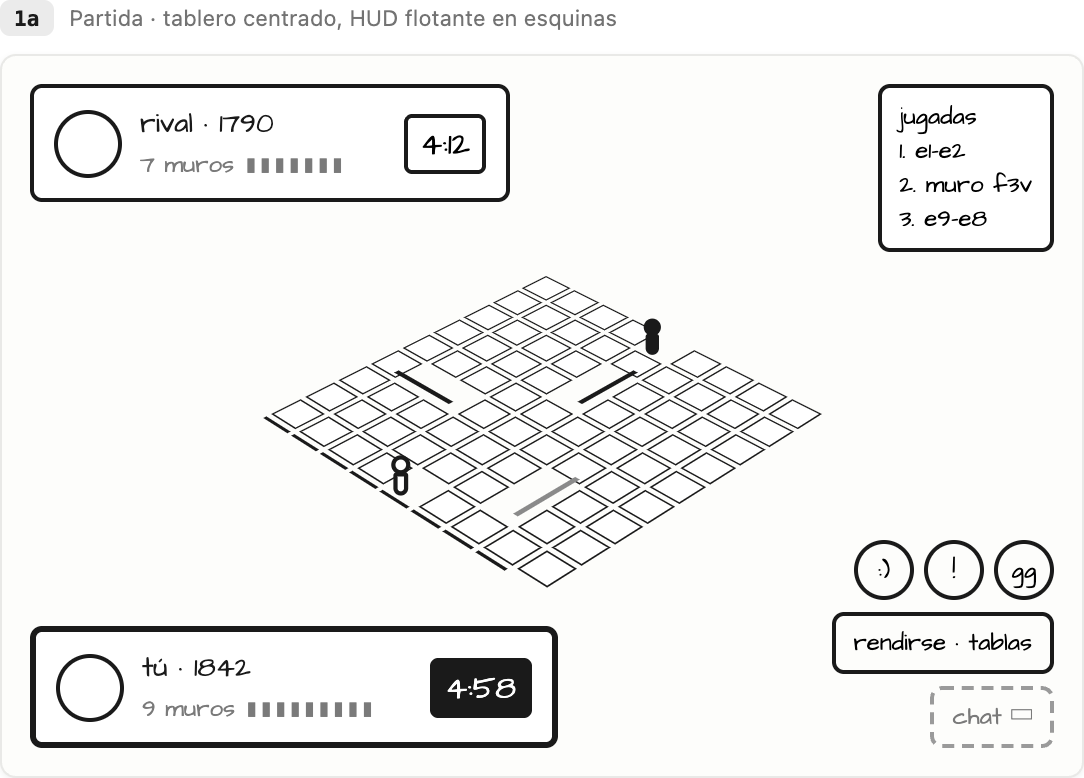
\includegraphics[width=\linewidth]{Prototipos/1a}\par\smallskip
{\footnotesize\RaggedRight \textbf{1a: Partida · tablero centrado, HUD flotante en esquinas}\par Motivo: Iteración anterior del HUD de partida, sustituida por las pantallas 20 y 21, que son las que describe el documento de diseño.\par Sustituida por: 20a, Partida · peón seleccionado.\par}
\end{minipage}\hfill
\begin{minipage}[t]{0.48\textwidth}
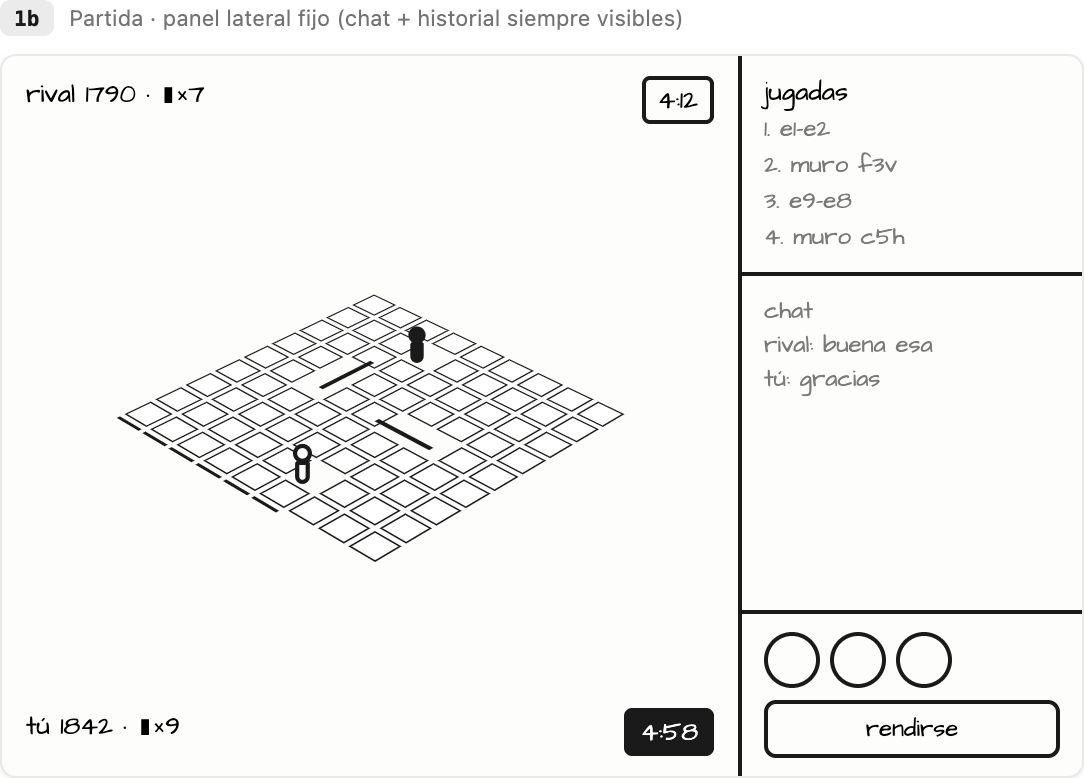
\includegraphics[width=\linewidth]{Prototipos/1b}\par\smallskip
{\footnotesize\RaggedRight \textbf{1b: Partida · panel lateral fijo con chat e historial}\par Motivo: Iteración anterior del HUD de partida, sustituida por las pantallas 20 y 21, que son las que describe el documento de diseño.\par Sustituida por: 20a, Partida · peón seleccionado.\par}
\end{minipage}
\par
\par\medskip\noindent
\begin{minipage}[t]{0.48\textwidth}
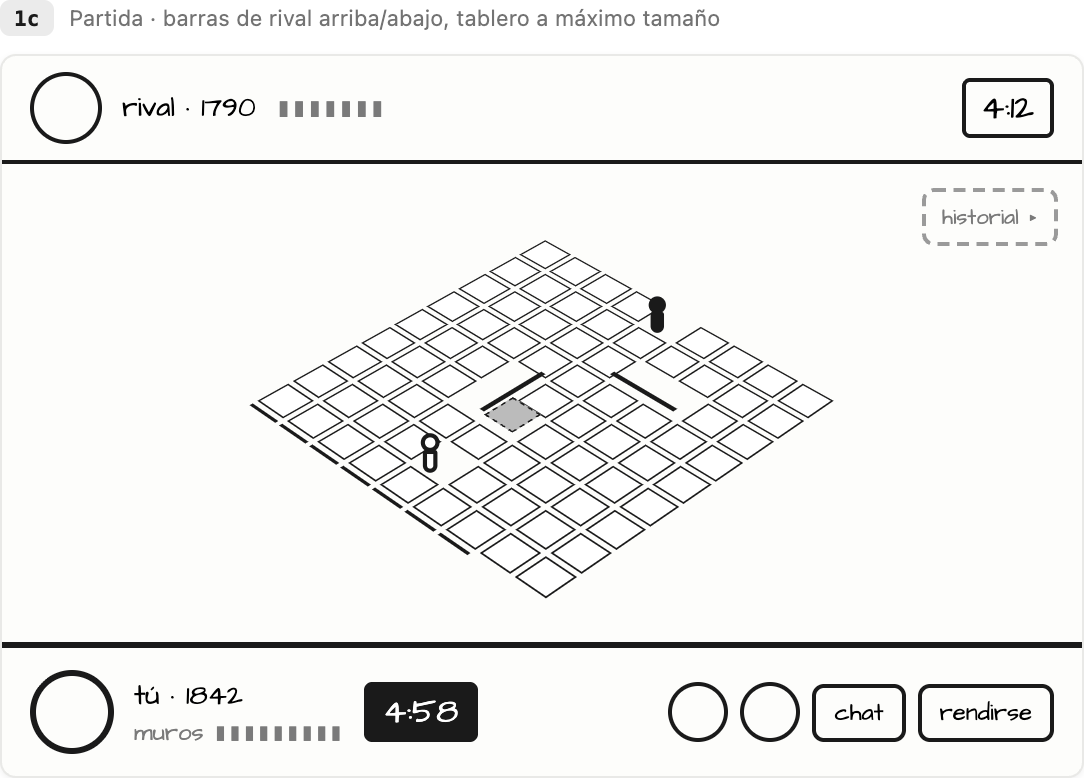
\includegraphics[width=\linewidth]{Prototipos/1c}\par\smallskip
{\footnotesize\RaggedRight \textbf{1c: Partida · barras de rival arriba y abajo}\par Motivo: Iteración anterior del HUD de partida, sustituida por las pantallas 20 y 21, que son las que describe el documento de diseño.\par Sustituida por: 20a, Partida · peón seleccionado.\par}
\end{minipage}\hfill
\begin{minipage}[t]{0.48\textwidth}
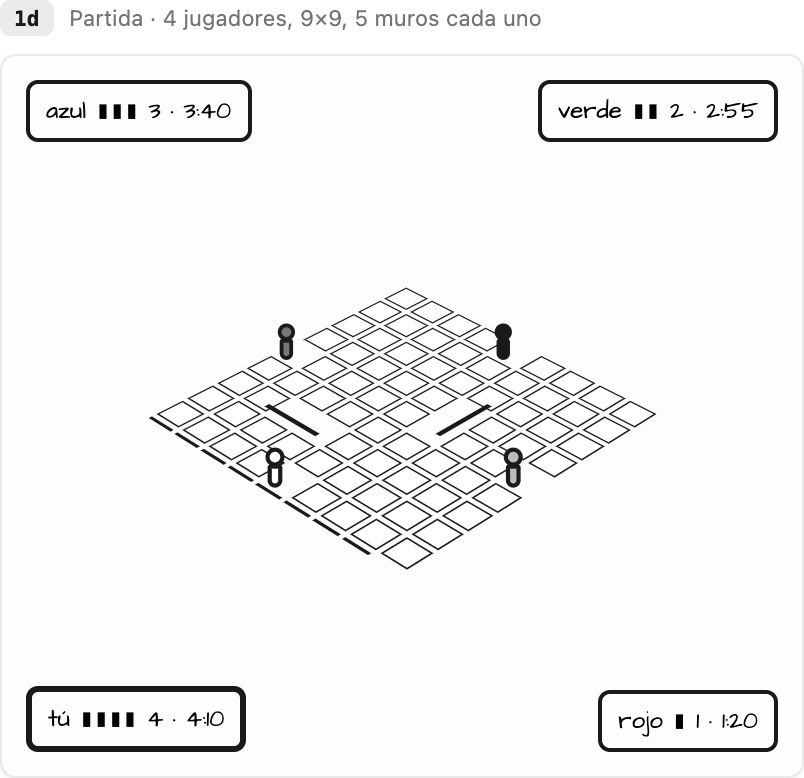
\includegraphics[width=\linewidth]{Prototipos/1d}\par\smallskip
{\footnotesize\RaggedRight \textbf{1d: Partida · 4 jugadores, 9×9, 5 muros cada uno}\par Motivo: Variante de modo del HUD anterior. El modo cambia el tablero y el número de jugadores, no los datos que se escriben.\par Sustituida por: 20a, Partida · peón seleccionado.\par}
\end{minipage}
\par
\par\medskip\noindent
\begin{minipage}[t]{0.48\textwidth}
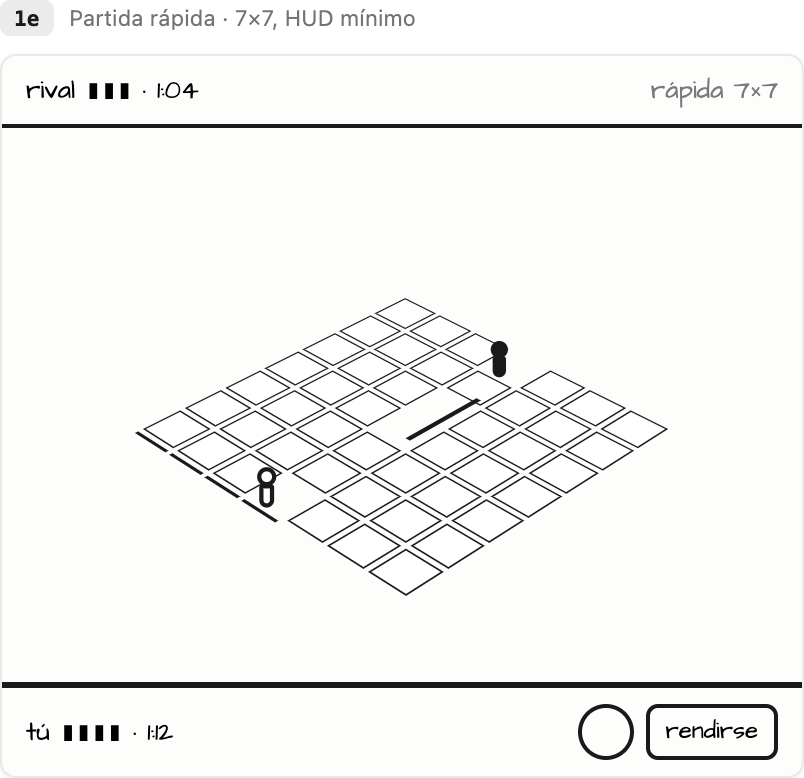
\includegraphics[width=\linewidth]{Prototipos/1e}\par\smallskip
{\footnotesize\RaggedRight \textbf{1e: Partida rápida · 7×7, HUD mínimo}\par Motivo: Variante de modo del HUD anterior. El modo cambia el tablero y el número de jugadores, no los datos que se escriben.\par Sustituida por: 20a, Partida · peón seleccionado.\par}
\end{minipage}\hfill
\begin{minipage}[t]{0.48\textwidth}
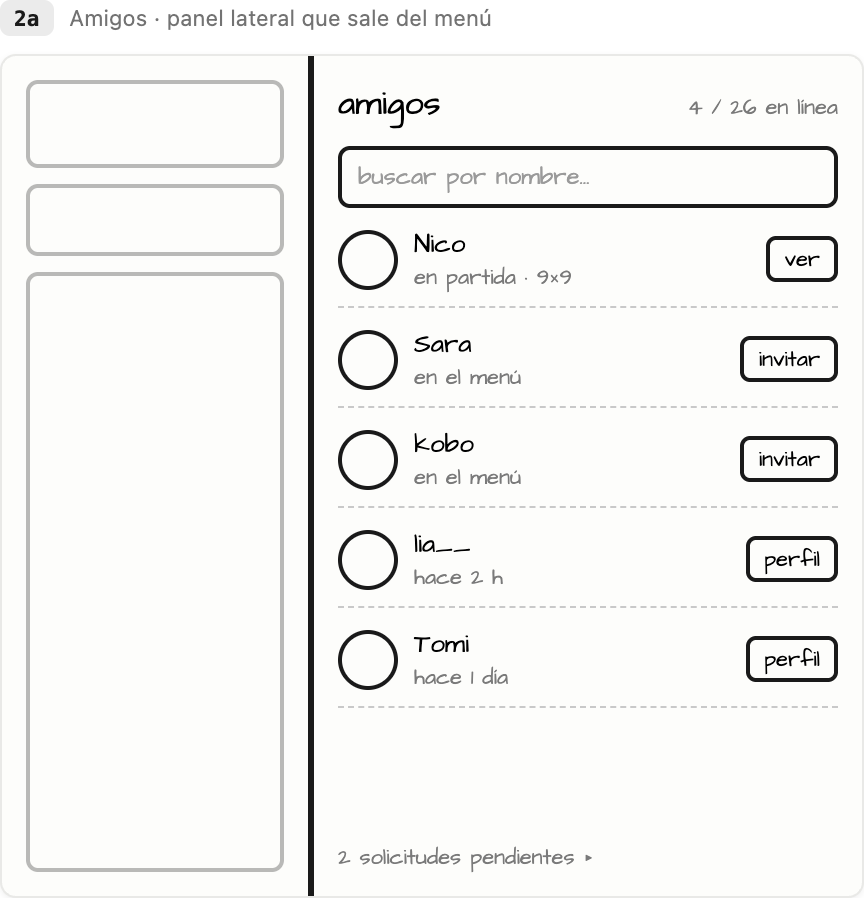
\includegraphics[width=\linewidth]{Prototipos/2a}\par\smallskip
{\footnotesize\RaggedRight \textbf{2a: Amigos · panel lateral}\par Motivo: Variante de disposición de una pantalla ya seleccionada. 2b incluye además la pestaña de solicitudes.\par Sustituida por: 2b, Amigos · pantalla completa con pestañas.\par}
\end{minipage}
\par
\par\medskip\noindent
\begin{minipage}[t]{0.48\textwidth}
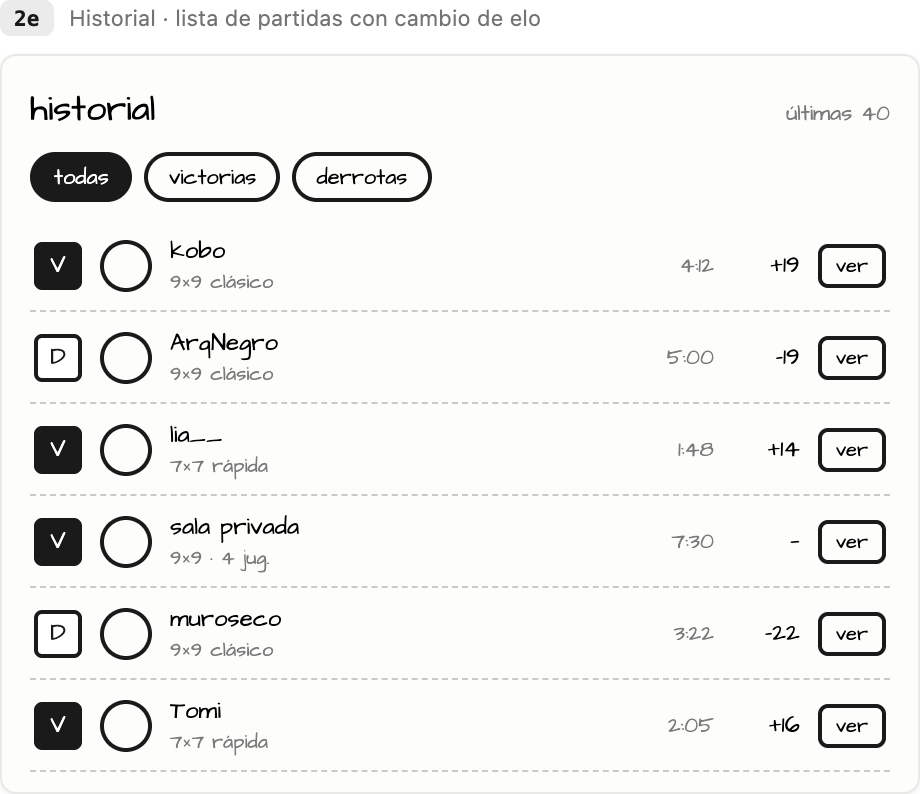
\includegraphics[width=\linewidth]{Prototipos/2e}\par\smallskip
{\footnotesize\RaggedRight \textbf{2e: Historial · lista con cambio de elo}\par Motivo: Versión anterior del historial, sin filtros por modo ni por forma de término.\par Sustituida por: 17f, Historial · filtros por modo y final.\par}
\end{minipage}\hfill
\begin{minipage}[t]{0.48\textwidth}
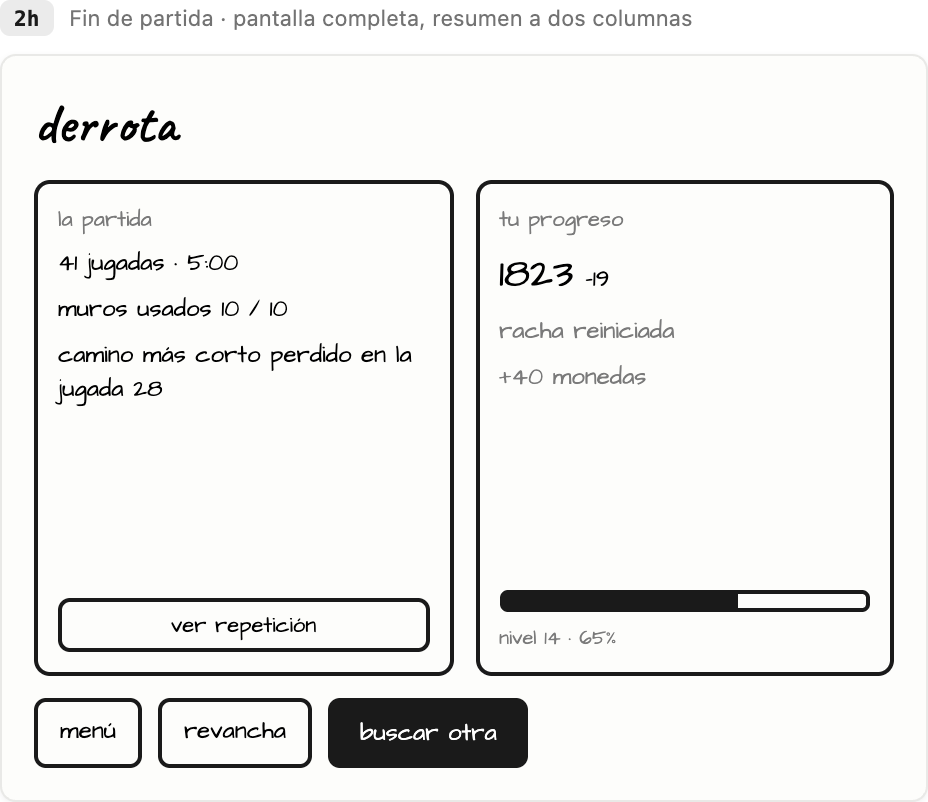
\includegraphics[width=\linewidth]{Prototipos/2h}\par\smallskip
{\footnotesize\RaggedRight \textbf{2h: Fin de partida · pantalla completa a dos columnas}\par Motivo: Variante de disposición de una pantalla ya seleccionada. El \mbox{CU-25} adopta la tarjeta sobre el tablero.\par Sustituida por: 2g, Fin de partida · tarjeta sobre el tablero.\par}
\end{minipage}
\par
\par\medskip\noindent
\begin{minipage}[t]{0.48\textwidth}
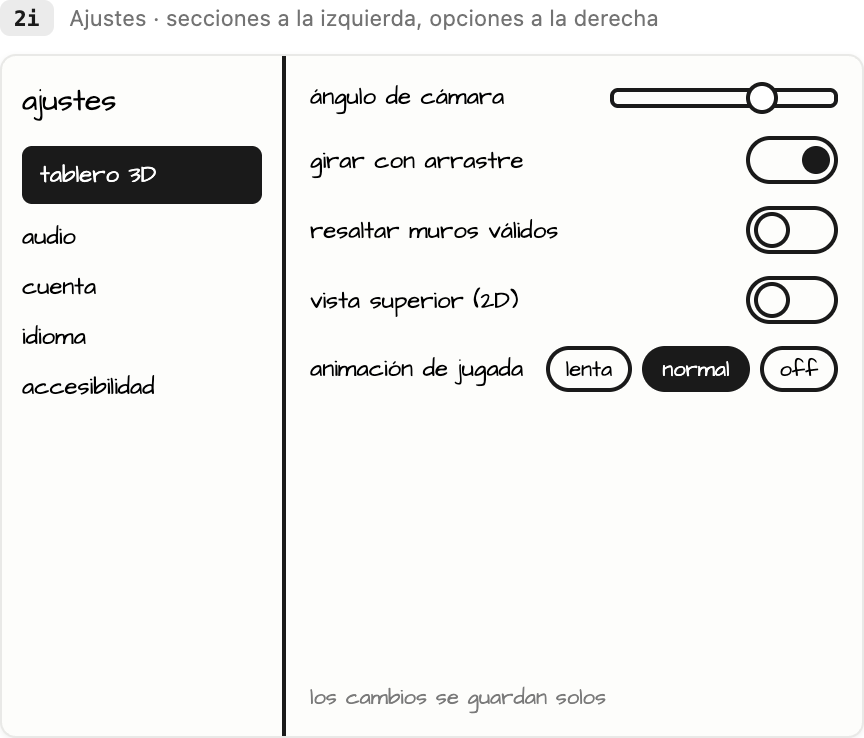
\includegraphics[width=\linewidth]{Prototipos/2i}\par\smallskip
{\footnotesize\RaggedRight \textbf{2i: Ajustes · secciones y opciones}\par Motivo: Configuración local del cliente: no llega a la base de datos.\par}
\end{minipage}\hfill
\begin{minipage}[t]{0.48\textwidth}
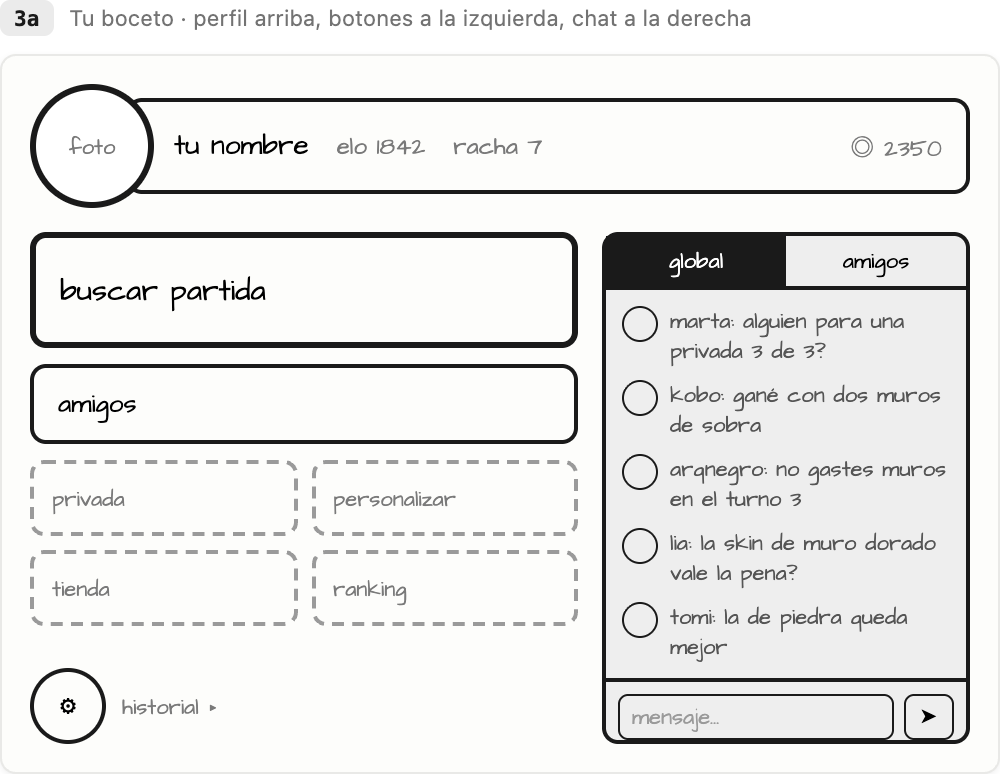
\includegraphics[width=\linewidth]{Prototipos/3a}\par\smallskip
{\footnotesize\RaggedRight \textbf{3a: Menú · boceto con chat a la derecha}\par Motivo: Variante de disposición de una pantalla ya seleccionada. Se prefiere 3b por ser más limpia: menos elementos simultáneos y el tablero 3D de fondo como identidad del juego.\par Sustituida por: 3b, Menú principal · tablero 3D de fondo.\par}
\end{minipage}
\par
\par\medskip\noindent
\begin{minipage}[t]{0.48\textwidth}
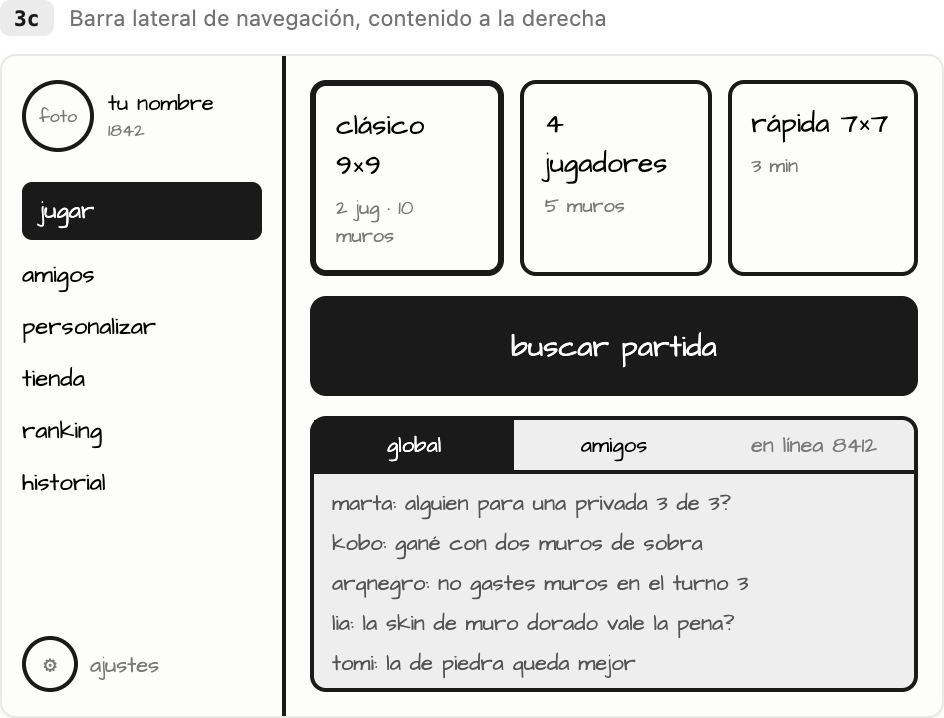
\includegraphics[width=\linewidth]{Prototipos/3c}\par\smallskip
{\footnotesize\RaggedRight \textbf{3c: Menú · barra lateral de navegación}\par Motivo: Variante de disposición de una pantalla ya seleccionada.\par Sustituida por: 3b, Menú principal · tablero 3D de fondo.\par}
\end{minipage}\hfill
\begin{minipage}[t]{0.48\textwidth}
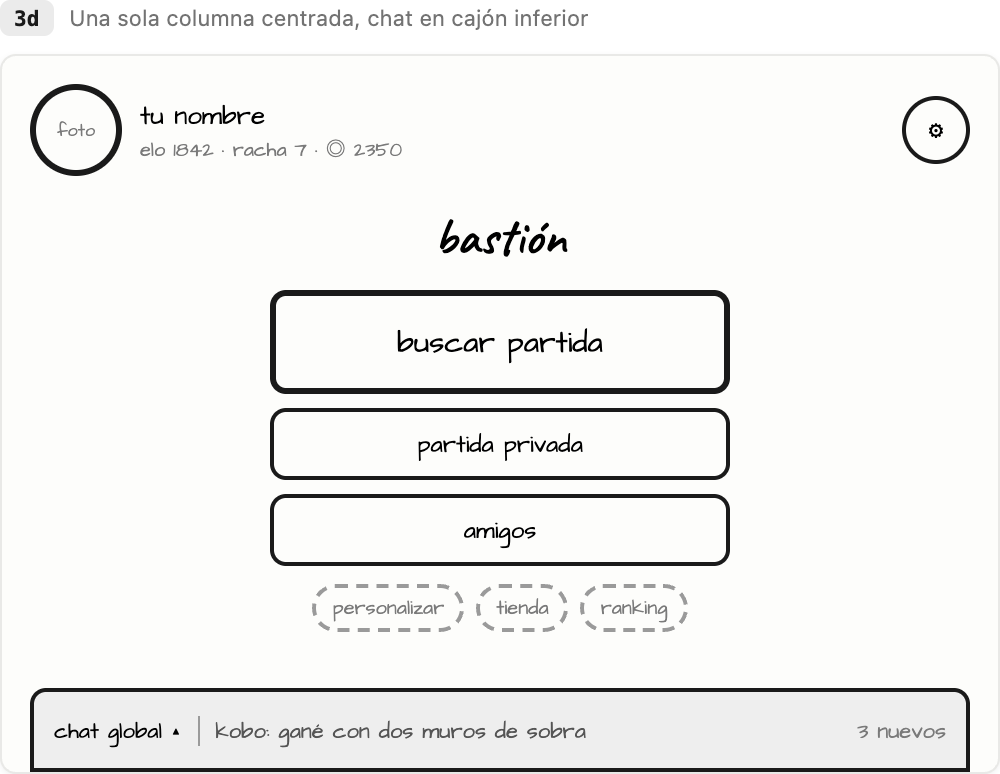
\includegraphics[width=\linewidth]{Prototipos/3d}\par\smallskip
{\footnotesize\RaggedRight \textbf{3d: Menú · una sola columna centrada}\par Motivo: Variante de disposición de una pantalla ya seleccionada.\par Sustituida por: 3b, Menú principal · tablero 3D de fondo.\par}
\end{minipage}
\par
\par\medskip\noindent
\begin{minipage}[t]{0.48\textwidth}
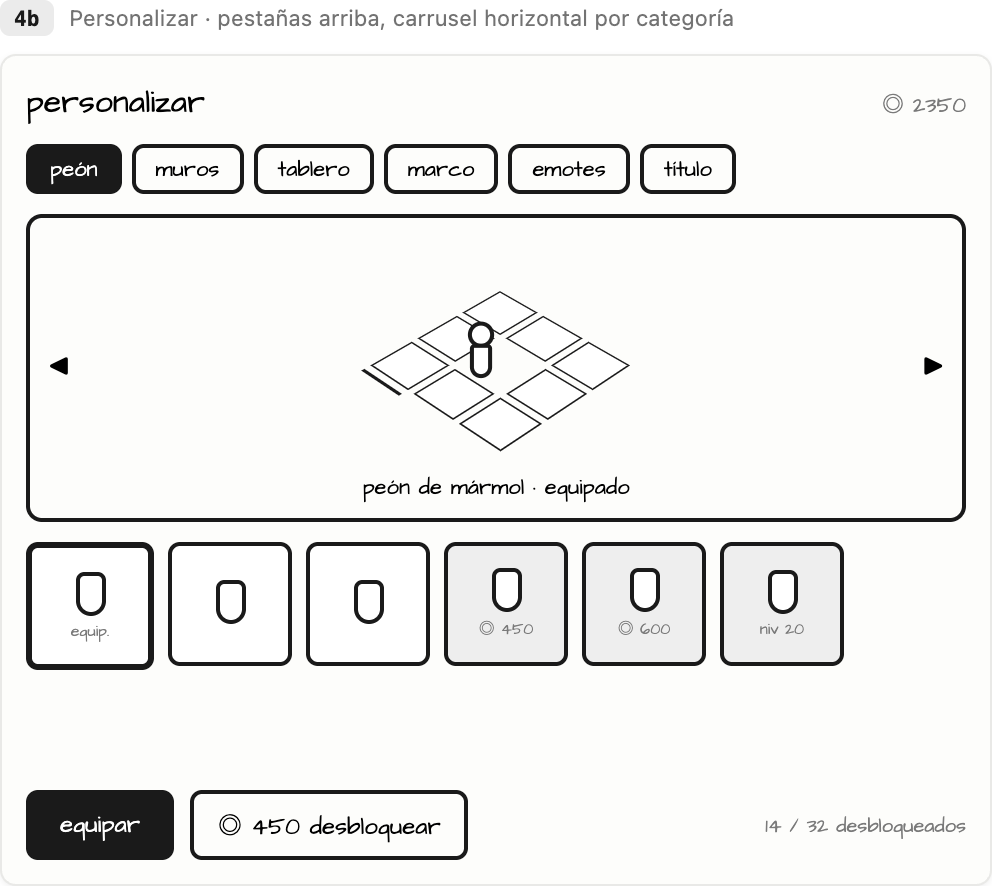
\includegraphics[width=\linewidth]{Prototipos/4b}\par\smallskip
{\footnotesize\RaggedRight \textbf{4b: Personalizar · pestañas y carrusel}\par Motivo: Variante de disposición de una pantalla ya seleccionada.\par Sustituida por: 4a, Personalizar · vista previa 3D y rejilla.\par}
\end{minipage}\hfill
\begin{minipage}[t]{0.48\textwidth}
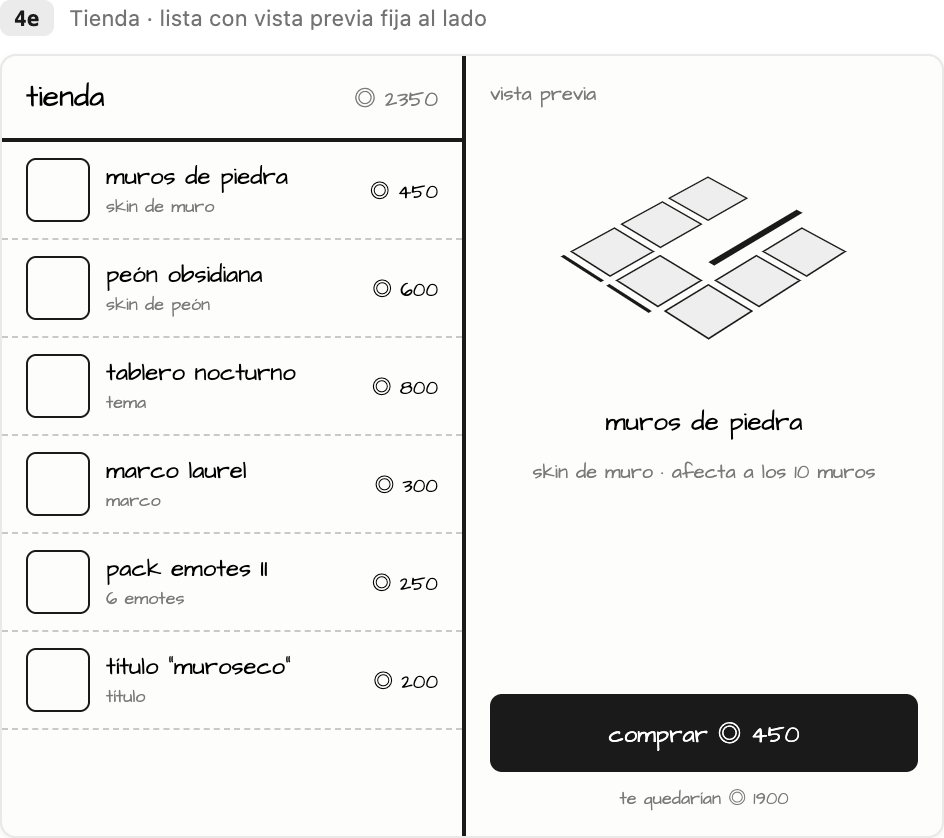
\includegraphics[width=\linewidth]{Prototipos/4e}\par\smallskip
{\footnotesize\RaggedRight \textbf{4e: Tienda · lista con vista previa}\par Motivo: Variante de disposición de una pantalla ya seleccionada.\par Sustituida por: 4d, Tienda · destacado y rejilla.\par}
\end{minipage}
\par
\par\medskip\noindent
\begin{minipage}[t]{0.48\textwidth}
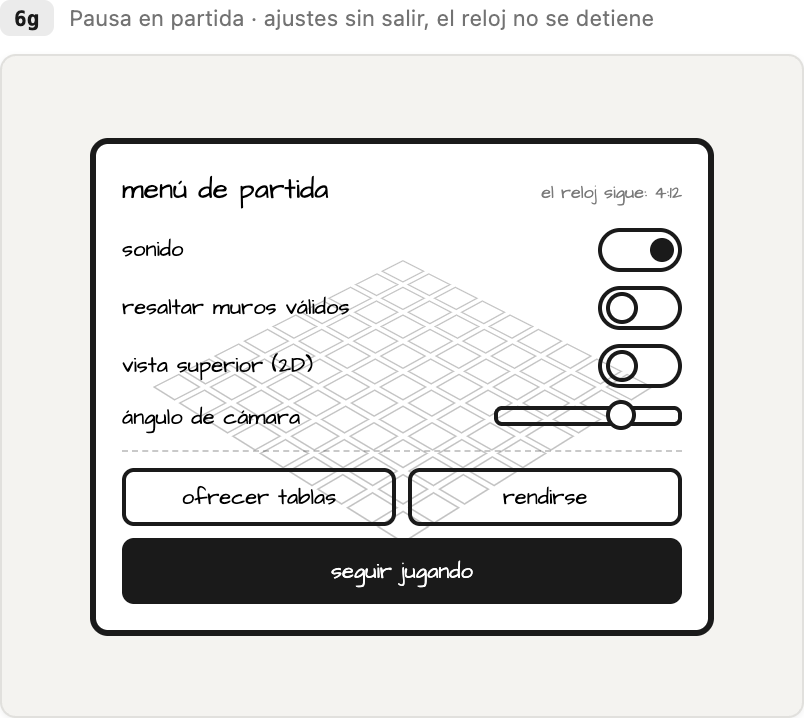
\includegraphics[width=\linewidth]{Prototipos/6g}\par\smallskip
{\footnotesize\RaggedRight \textbf{6g: Pausa en partida}\par Motivo: Estado visual de la partida sin operación de datos propia. El reloj no se detiene y no se guarda nada.\par}
\end{minipage}\hfill
\begin{minipage}[t]{0.48\textwidth}
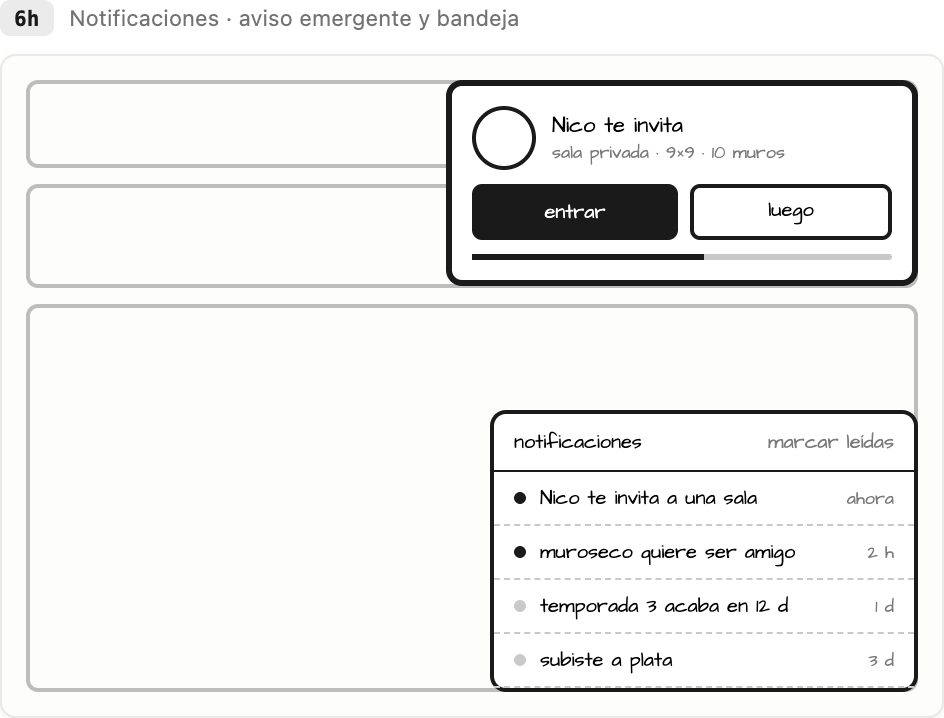
\includegraphics[width=\linewidth]{Prototipos/6h}\par\smallskip
{\footnotesize\RaggedRight \textbf{6h: Notificaciones}\par Motivo: Transversal: cada funcionalidad que notifica lo resuelve en su propio caso de uso.\par}
\end{minipage}
\par
\par\medskip\noindent
\begin{minipage}[t]{0.48\textwidth}
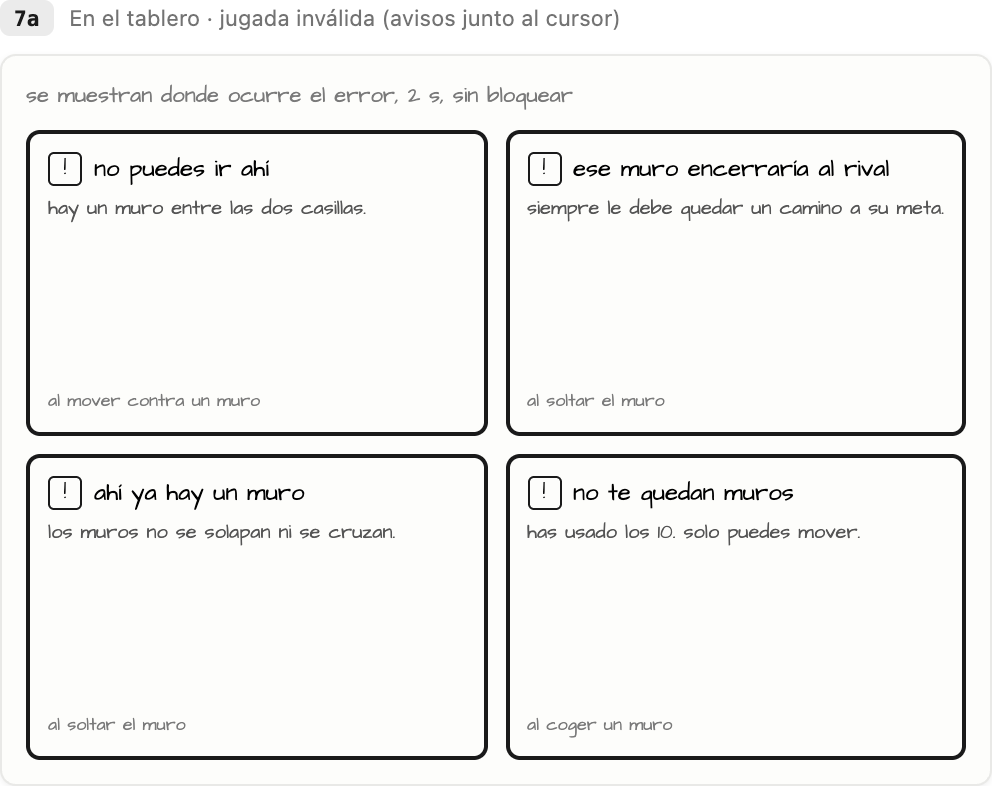
\includegraphics[width=\linewidth]{Prototipos/7a}\par\smallskip
{\footnotesize\RaggedRight \textbf{7a: Errores · jugada inválida}\par Motivo: Catálogo de mensajes de error y aviso. Documenta los flujos alternos y las excepciones de los casos de uso, no una operación sobre datos.\par}
\end{minipage}\hfill
\begin{minipage}[t]{0.48\textwidth}
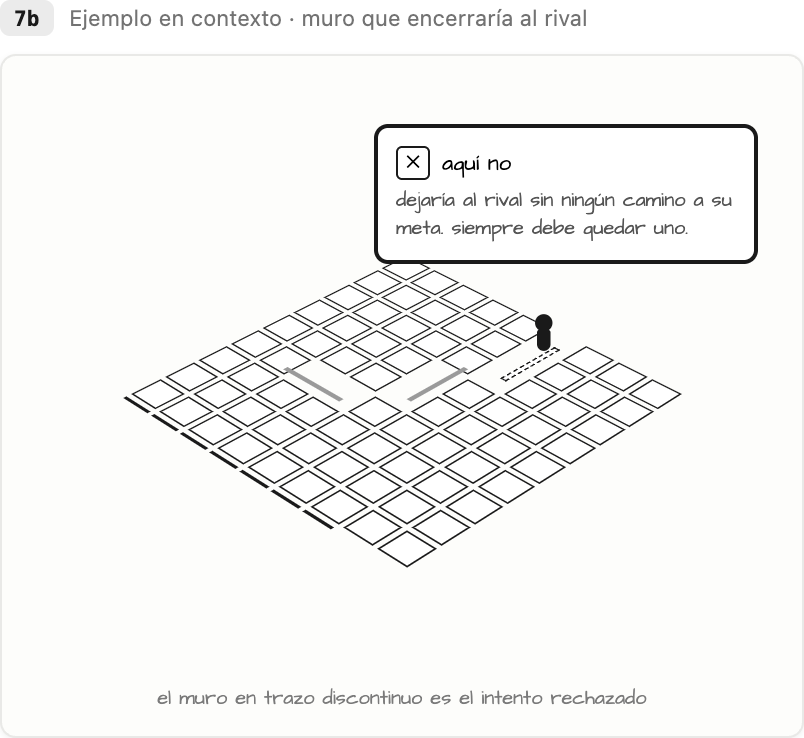
\includegraphics[width=\linewidth]{Prototipos/7b}\par\smallskip
{\footnotesize\RaggedRight \textbf{7b: Errores · muro que encerraría al rival}\par Motivo: Catálogo de mensajes de error y aviso. Documenta los flujos alternos y las excepciones de los casos de uso, no una operación sobre datos.\par}
\end{minipage}
\par
\par\medskip\noindent
\begin{minipage}[t]{0.48\textwidth}
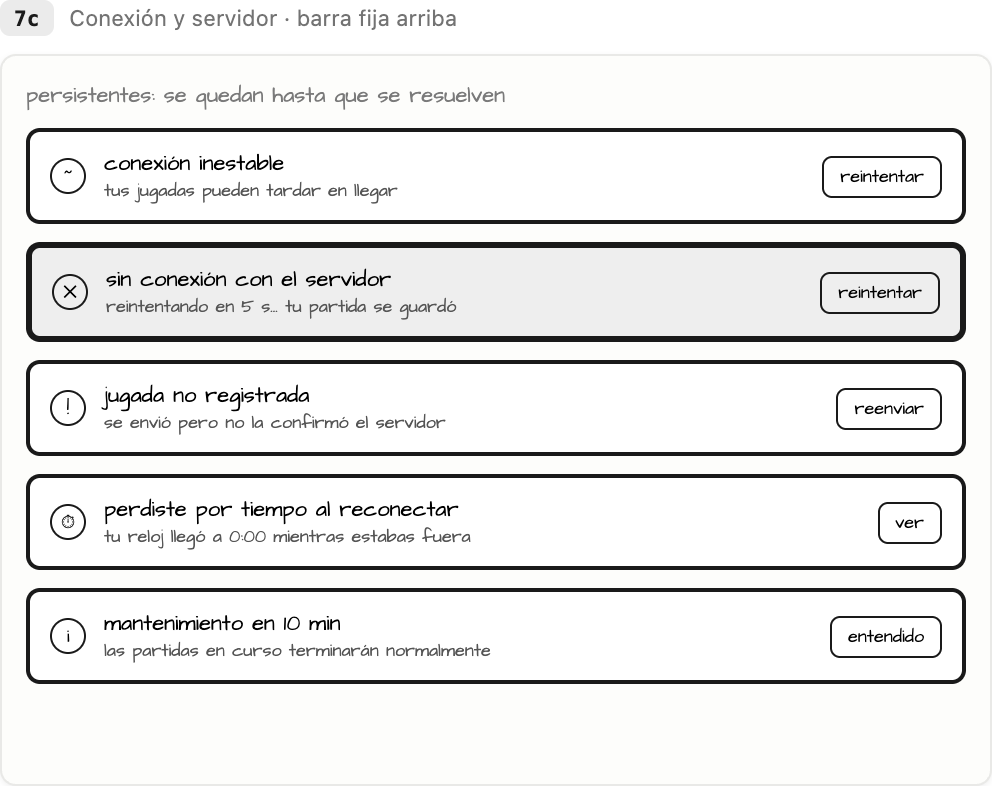
\includegraphics[width=\linewidth]{Prototipos/7c}\par\smallskip
{\footnotesize\RaggedRight \textbf{7c: Errores · conexión y servidor}\par Motivo: Catálogo de mensajes de error y aviso. Documenta los flujos alternos y las excepciones de los casos de uso, no una operación sobre datos.\par}
\end{minipage}\hfill
\begin{minipage}[t]{0.48\textwidth}
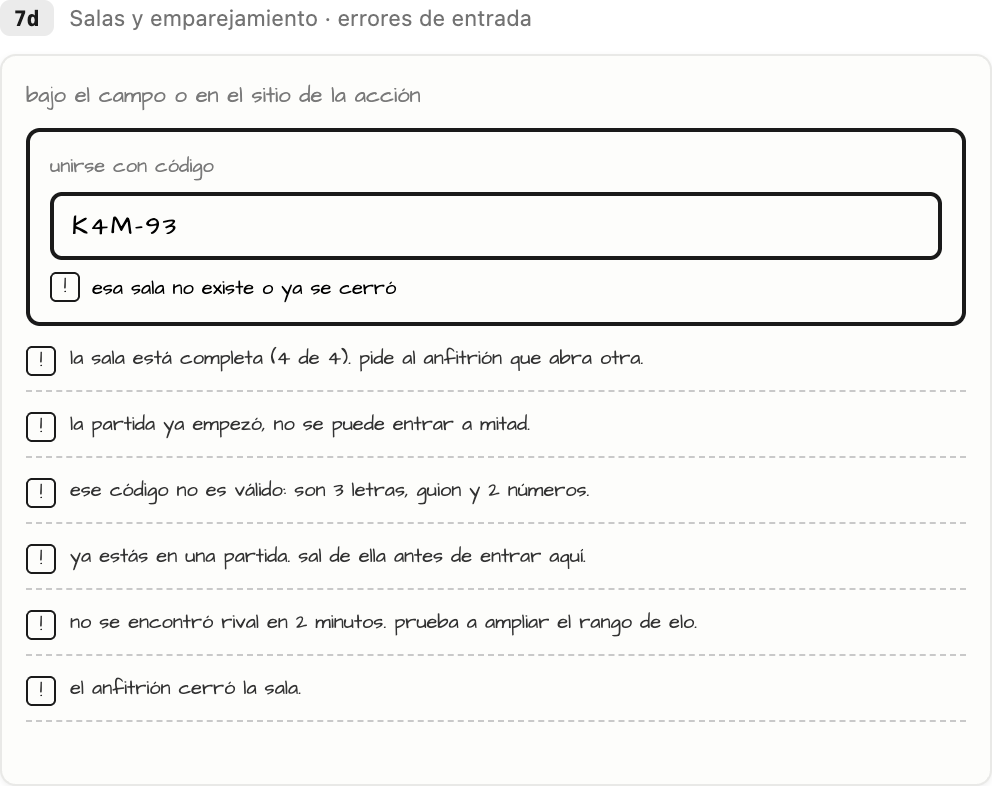
\includegraphics[width=\linewidth]{Prototipos/7d}\par\smallskip
{\footnotesize\RaggedRight \textbf{7d: Errores · salas y emparejamiento}\par Motivo: Catálogo de mensajes de error y aviso. Documenta los flujos alternos y las excepciones de los casos de uso, no una operación sobre datos.\par}
\end{minipage}
\par
\par\medskip\noindent
\begin{minipage}[t]{0.48\textwidth}
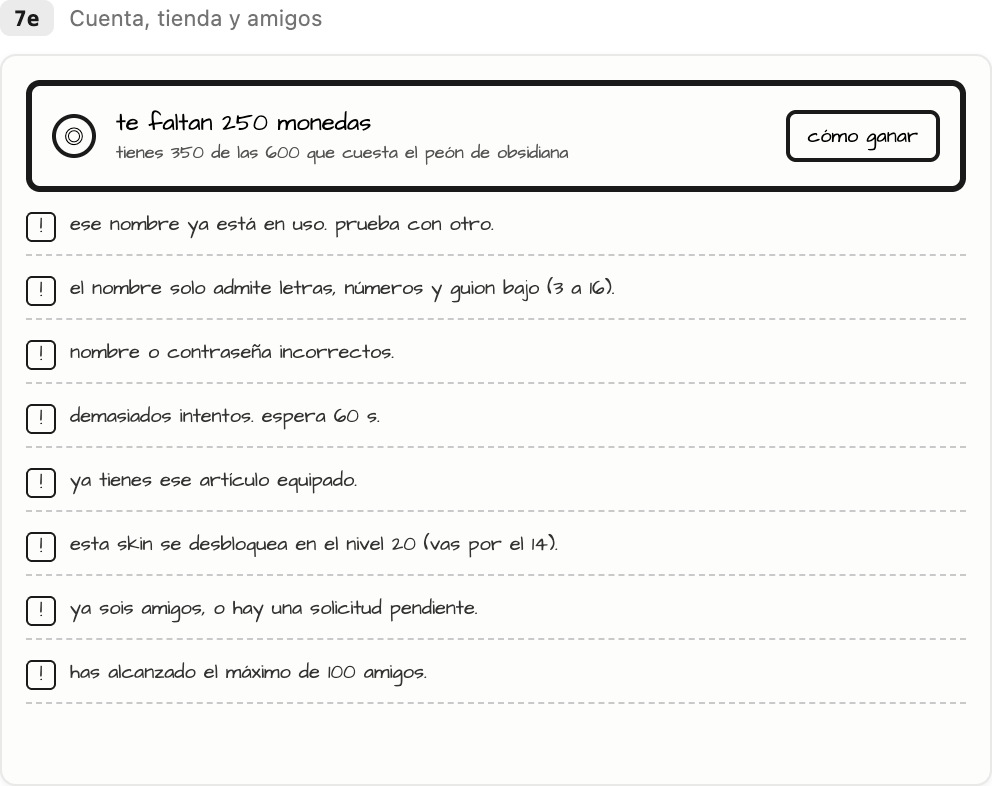
\includegraphics[width=\linewidth]{Prototipos/7e}\par\smallskip
{\footnotesize\RaggedRight \textbf{7e: Errores · cuenta, tienda y amigos}\par Motivo: Catálogo de mensajes de error y aviso. Documenta los flujos alternos y las excepciones de los casos de uso, no una operación sobre datos.\par}
\end{minipage}\hfill
\begin{minipage}[t]{0.48\textwidth}
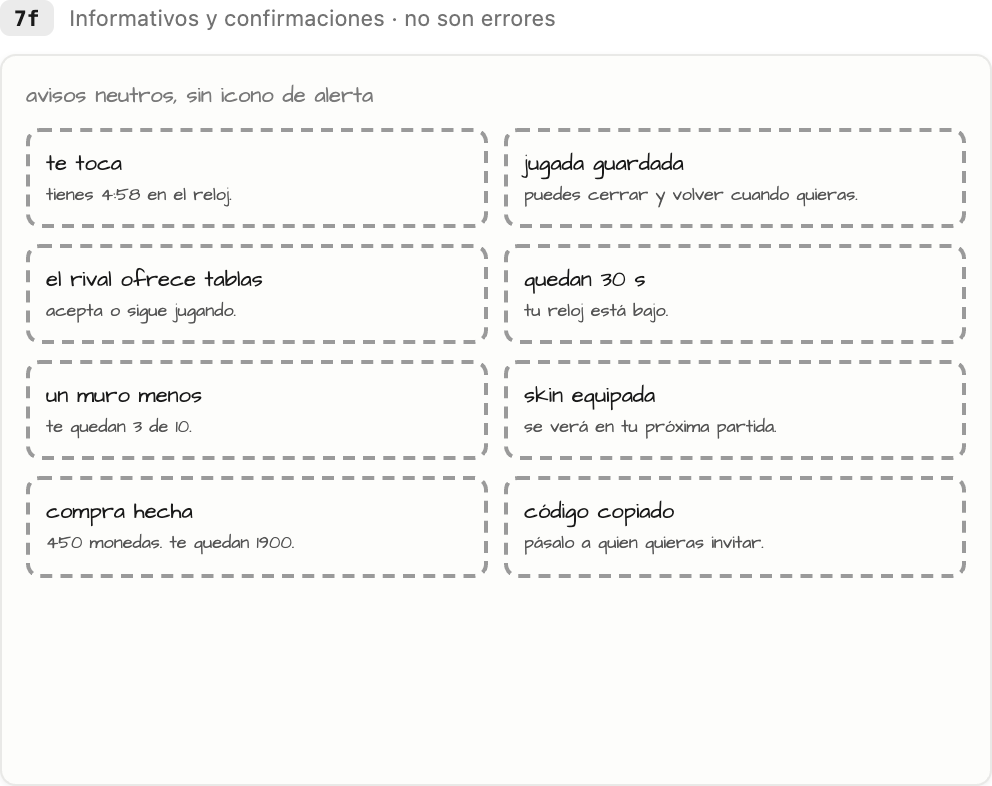
\includegraphics[width=\linewidth]{Prototipos/7f}\par\smallskip
{\footnotesize\RaggedRight \textbf{7f: Avisos informativos y confirmaciones}\par Motivo: Catálogo de mensajes de error y aviso. Documenta los flujos alternos y las excepciones de los casos de uso, no una operación sobre datos.\par}
\end{minipage}
\par
\par\medskip\noindent
\begin{minipage}[t]{0.48\textwidth}
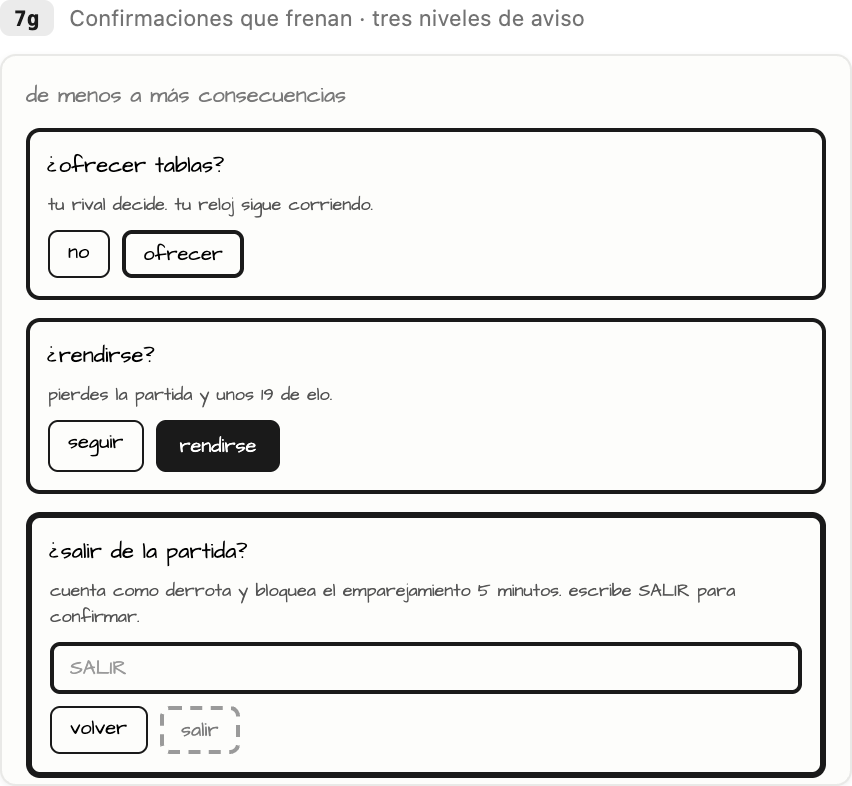
\includegraphics[width=\linewidth]{Prototipos/7g}\par\smallskip
{\footnotesize\RaggedRight \textbf{7g: Confirmaciones que frenan}\par Motivo: Catálogo de mensajes de error y aviso. Documenta los flujos alternos y las excepciones de los casos de uso, no una operación sobre datos.\par}
\end{minipage}\hfill
\begin{minipage}[t]{0.48\textwidth}
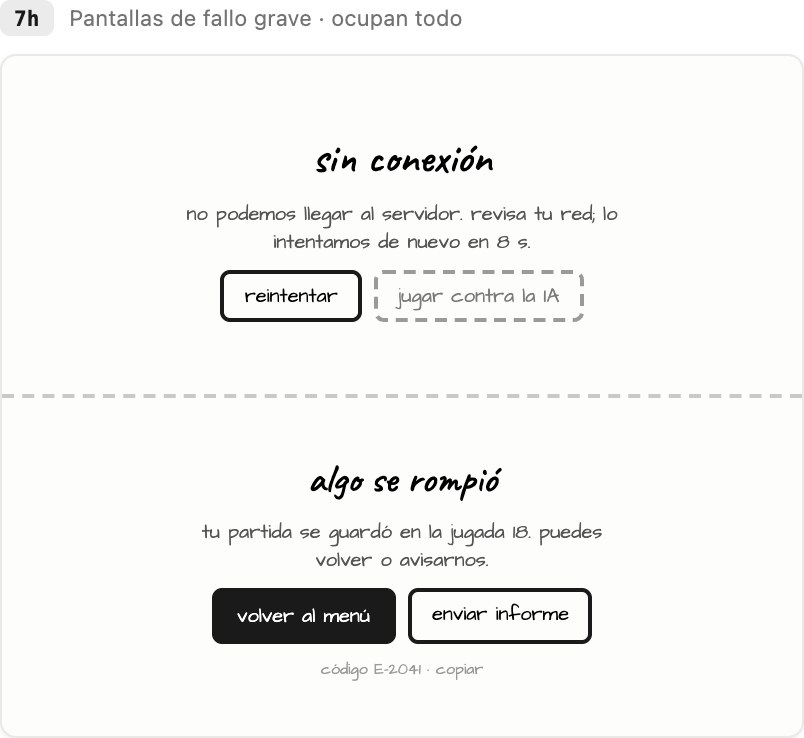
\includegraphics[width=\linewidth]{Prototipos/7h}\par\smallskip
{\footnotesize\RaggedRight \textbf{7h: Pantallas de fallo grave}\par Motivo: Catálogo de mensajes de error y aviso. Documenta los flujos alternos y las excepciones de los casos de uso, no una operación sobre datos.\par}
\end{minipage}
\par
\par\medskip\noindent
\begin{minipage}[t]{0.48\textwidth}
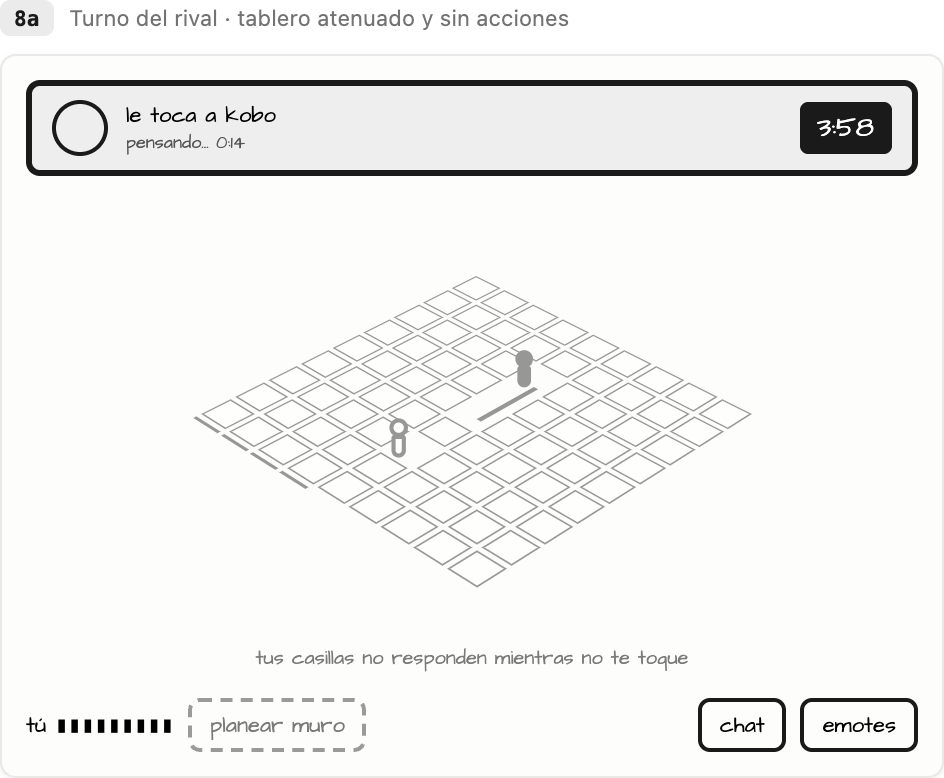
\includegraphics[width=\linewidth]{Prototipos/8a}\par\smallskip
{\footnotesize\RaggedRight \textbf{8a: Turno del rival}\par Motivo: Estado visual de la partida sin operación de datos propia.\par}
\end{minipage}\hfill
\begin{minipage}[t]{0.48\textwidth}
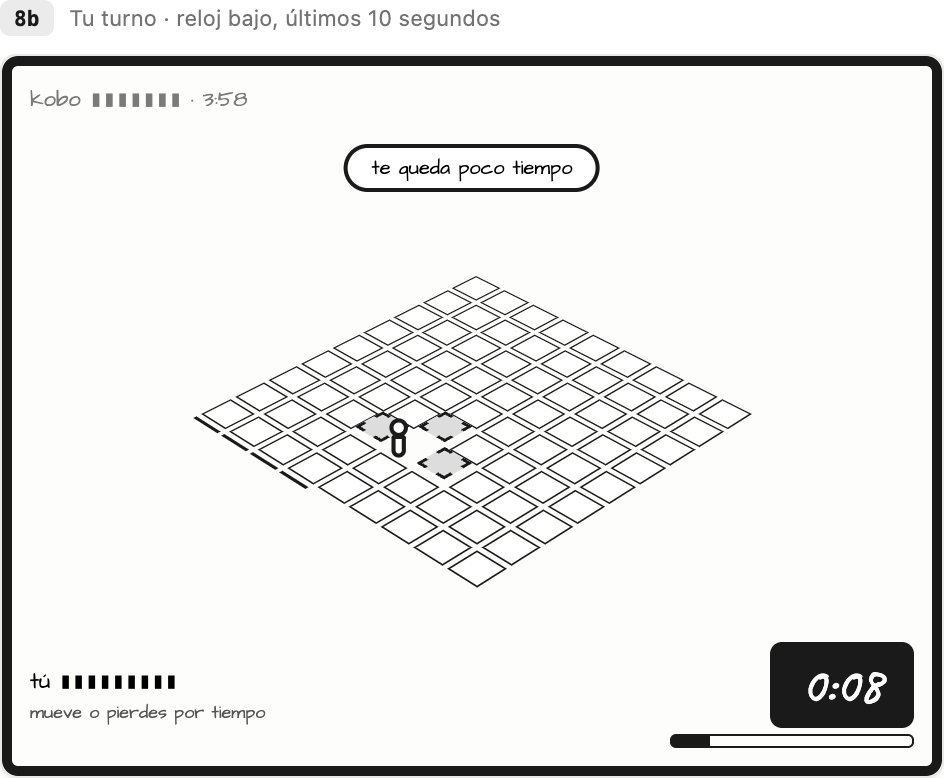
\includegraphics[width=\linewidth]{Prototipos/8b}\par\smallskip
{\footnotesize\RaggedRight \textbf{8b: Tu turno · últimos 10 segundos}\par Motivo: Estado visual de la partida sin operación de datos propia.\par}
\end{minipage}
\par
\par\medskip\noindent
\begin{minipage}[t]{0.48\textwidth}
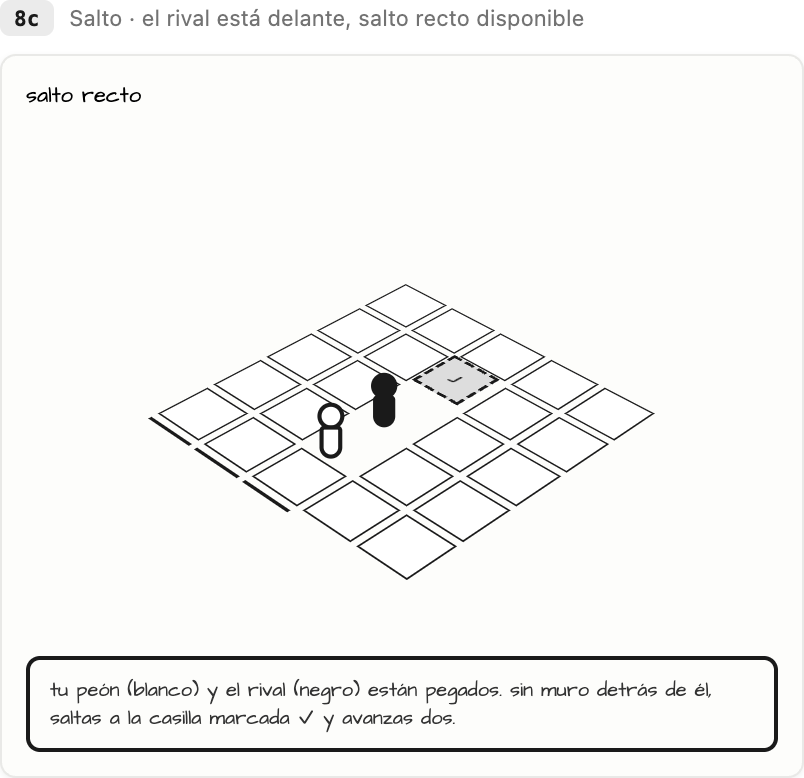
\includegraphics[width=\linewidth]{Prototipos/8c}\par\smallskip
{\footnotesize\RaggedRight \textbf{8c: Salto recto}\par Motivo: Regla visual del salto; registra la misma Jugada que un movimiento.\par Sustituida por: 20a, Partida · peón seleccionado.\par}
\end{minipage}\hfill
\begin{minipage}[t]{0.48\textwidth}
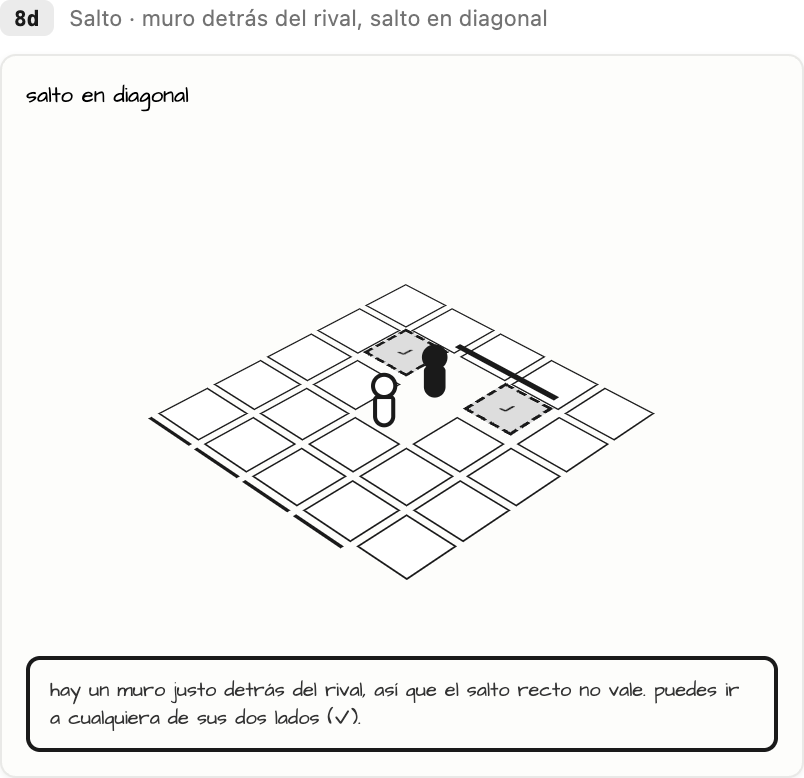
\includegraphics[width=\linewidth]{Prototipos/8d}\par\smallskip
{\footnotesize\RaggedRight \textbf{8d: Salto en diagonal}\par Motivo: Regla visual del salto; registra la misma Jugada que un movimiento.\par Sustituida por: 20a, Partida · peón seleccionado.\par}
\end{minipage}
\par
\par\medskip\noindent
\begin{minipage}[t]{0.48\textwidth}
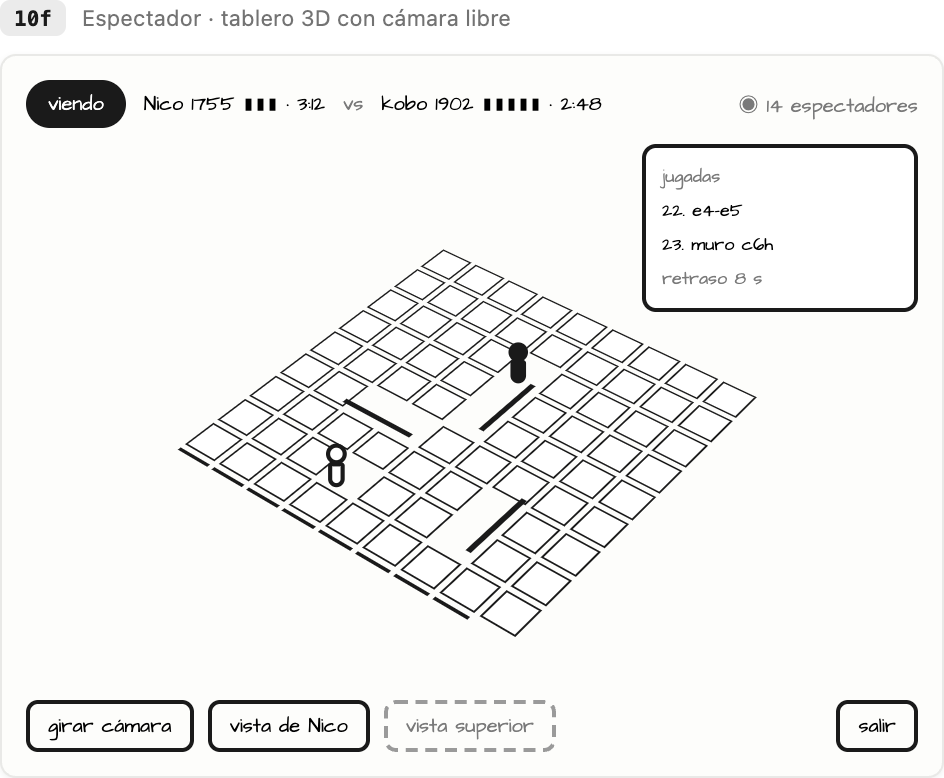
\includegraphics[width=\linewidth]{Prototipos/10f}\par\smallskip
{\footnotesize\RaggedRight \textbf{10f: Espectador · cámara libre}\par Motivo: Variante de disposición de una pantalla ya seleccionada. 10g añade el chat de espectadores, que escribe en la base de datos.\par Sustituida por: 10g, Espectador · con chat de espectadores.\par}
\end{minipage}\hfill
\begin{minipage}[t]{0.48\textwidth}
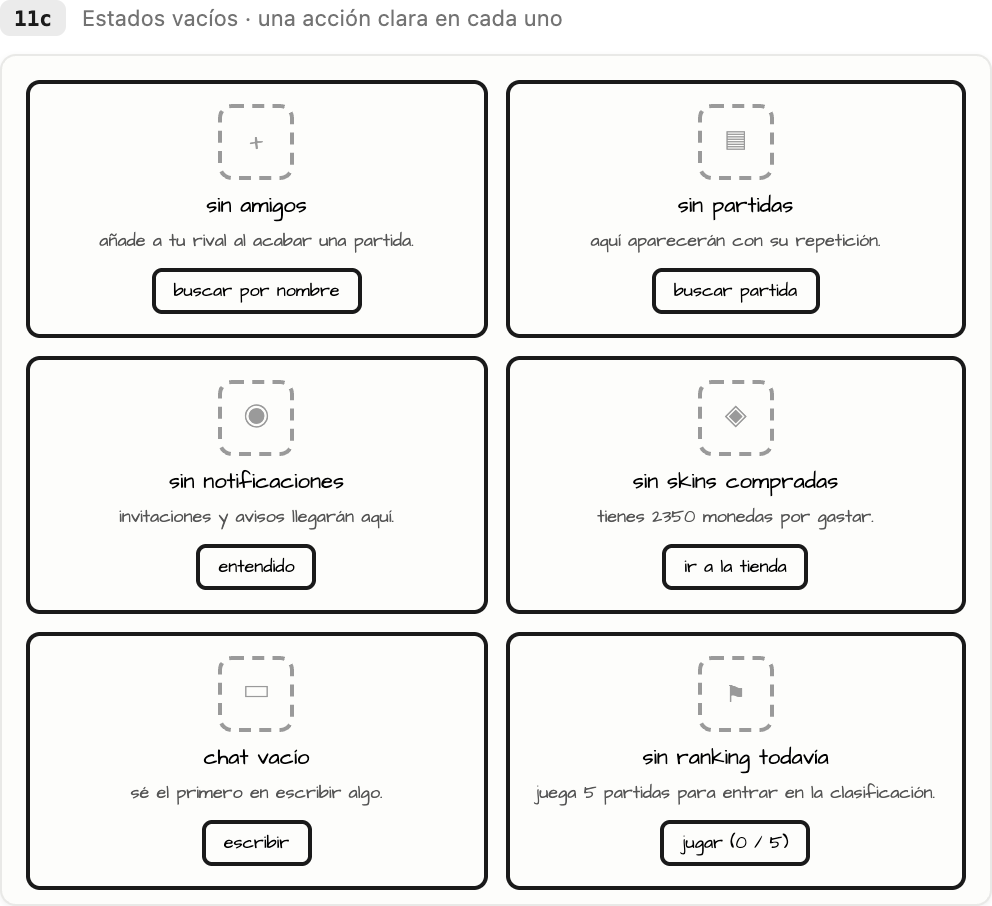
\includegraphics[width=\linewidth]{Prototipos/11c}\par\smallskip
{\footnotesize\RaggedRight \textbf{11c: Estados vacíos}\par Motivo: Estado vacío genérico; no muestra datos.\par}
\end{minipage}
\par
\par\medskip\noindent
\begin{minipage}[t]{0.48\textwidth}
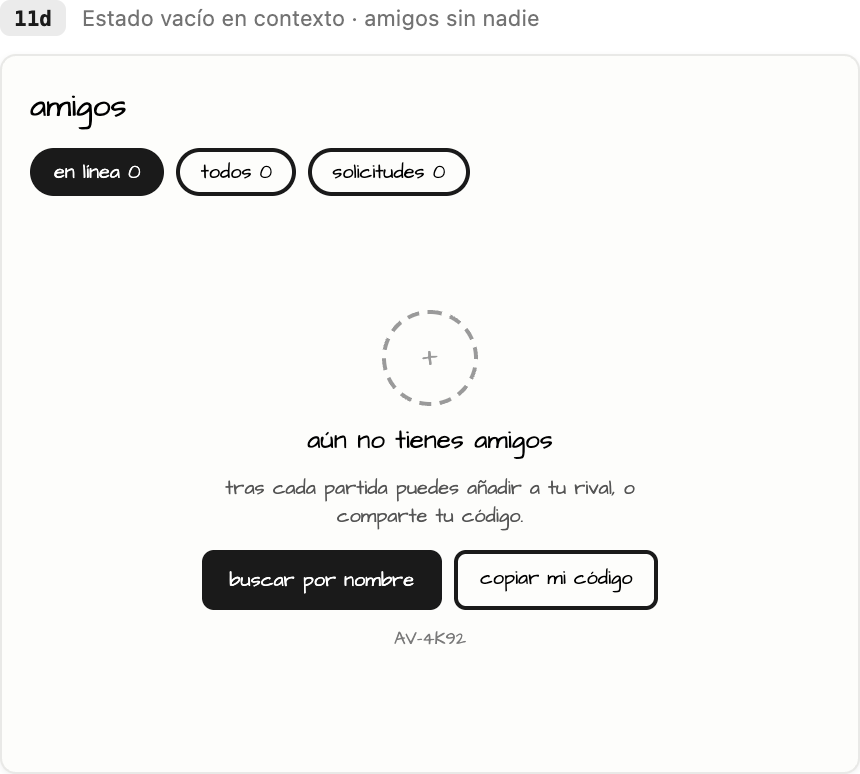
\includegraphics[width=\linewidth]{Prototipos/11d}\par\smallskip
{\footnotesize\RaggedRight \textbf{11d: Estado vacío en contexto}\par Motivo: Estado vacío genérico; no muestra datos.\par}
\end{minipage}\hfill
\begin{minipage}[t]{0.48\textwidth}
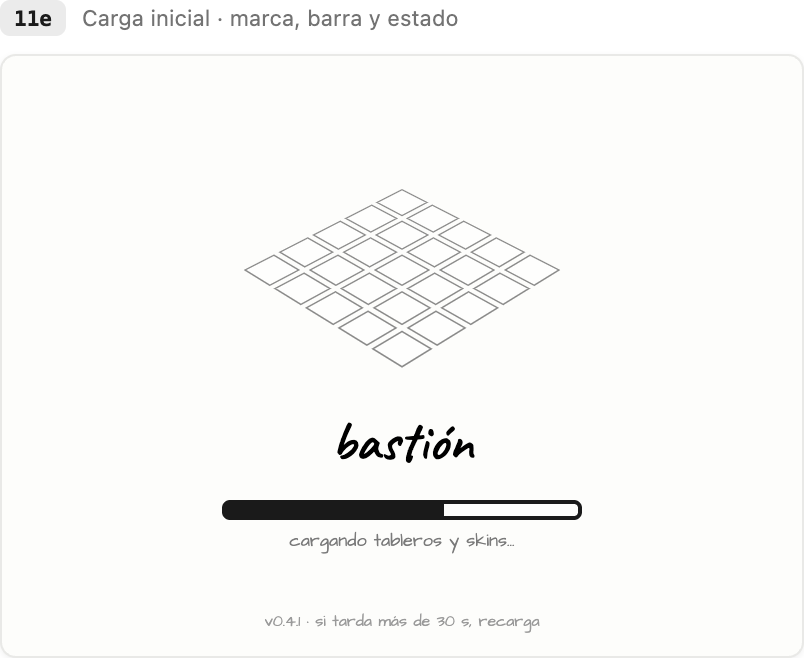
\includegraphics[width=\linewidth]{Prototipos/11e}\par\smallskip
{\footnotesize\RaggedRight \textbf{11e: Carga inicial}\par Motivo: Pantalla de carga; no muestra datos.\par}
\end{minipage}
\par
\par\medskip\noindent
\begin{minipage}[t]{0.48\textwidth}
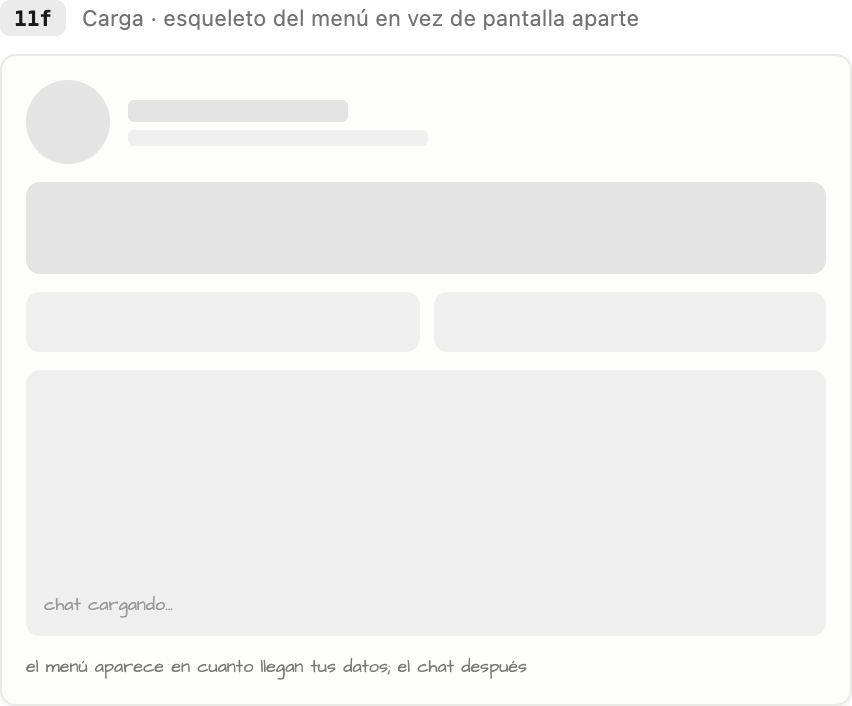
\includegraphics[width=\linewidth]{Prototipos/11f}\par\smallskip
{\footnotesize\RaggedRight \textbf{11f: Carga · esqueleto del menú}\par Motivo: Pantalla de carga; no muestra datos.\par}
\end{minipage}\hfill
\begin{minipage}[t]{0.48\textwidth}
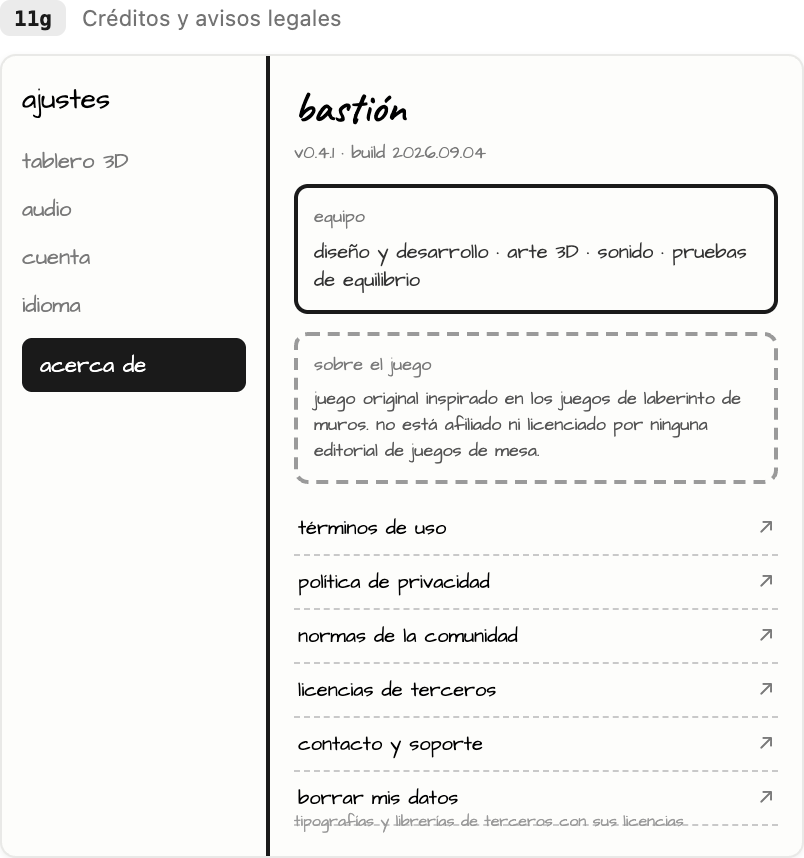
\includegraphics[width=\linewidth]{Prototipos/11g}\par\smallskip
{\footnotesize\RaggedRight \textbf{11g: Créditos y avisos legales}\par Motivo: Contenido estático.\par}
\end{minipage}
\par
\par\medskip\noindent
\begin{minipage}[t]{0.48\textwidth}
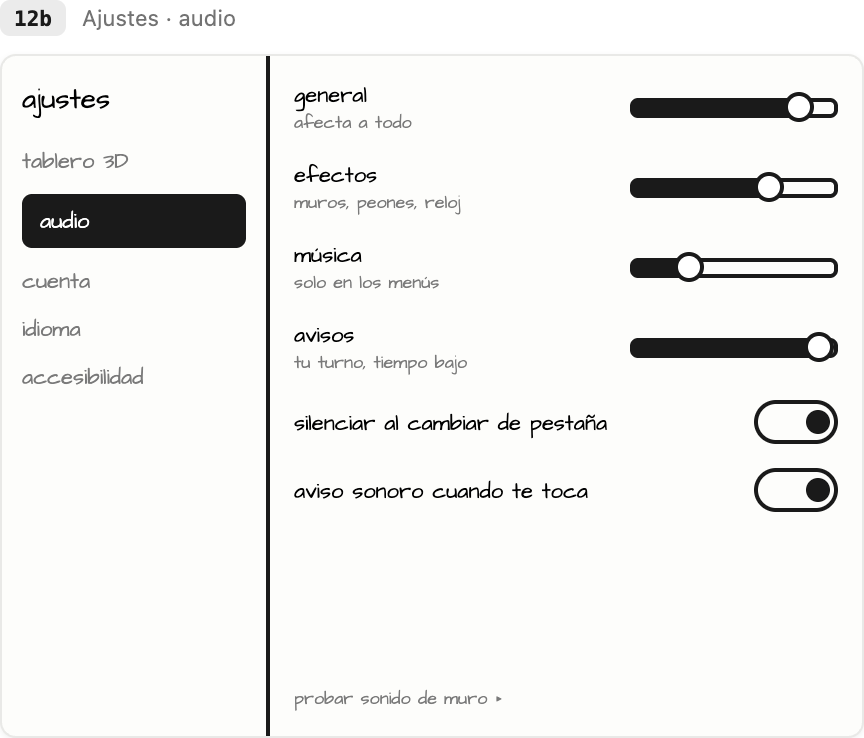
\includegraphics[width=\linewidth]{Prototipos/12b}\par\smallskip
{\footnotesize\RaggedRight \textbf{12b: Ajustes · audio}\par Motivo: Configuración local del cliente: no llega a la base de datos.\par}
\end{minipage}\hfill
\begin{minipage}[t]{0.48\textwidth}
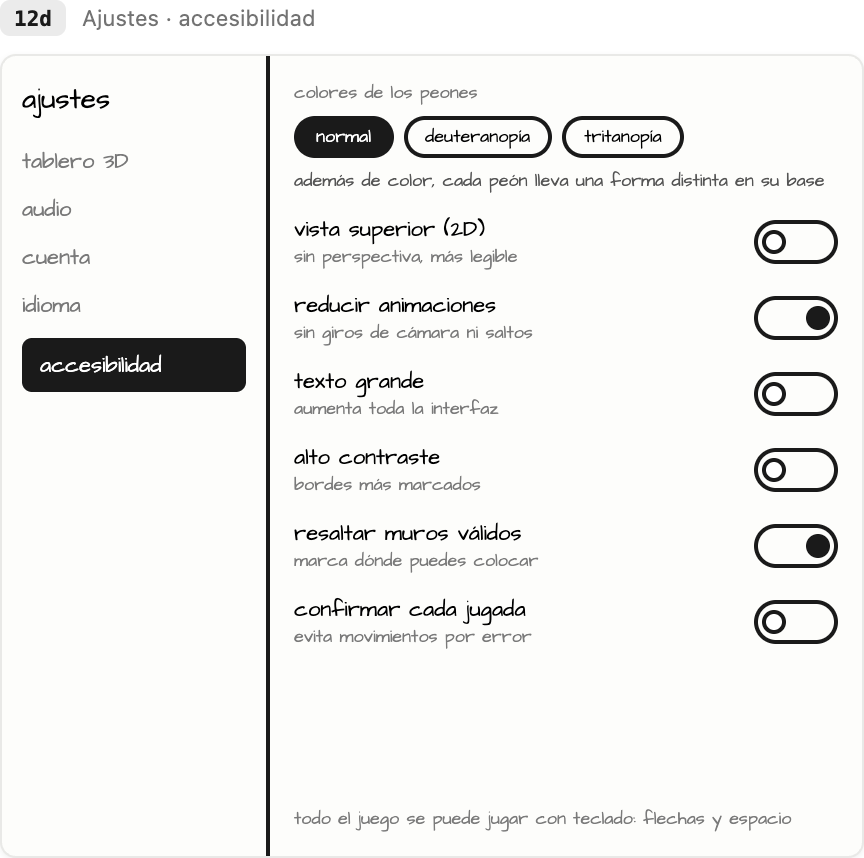
\includegraphics[width=\linewidth]{Prototipos/12d}\par\smallskip
{\footnotesize\RaggedRight \textbf{12d: Ajustes · accesibilidad}\par Motivo: Configuración local del cliente: no llega a la base de datos.\par}
\end{minipage}
\par
\par\medskip\noindent
\begin{minipage}[t]{0.48\textwidth}
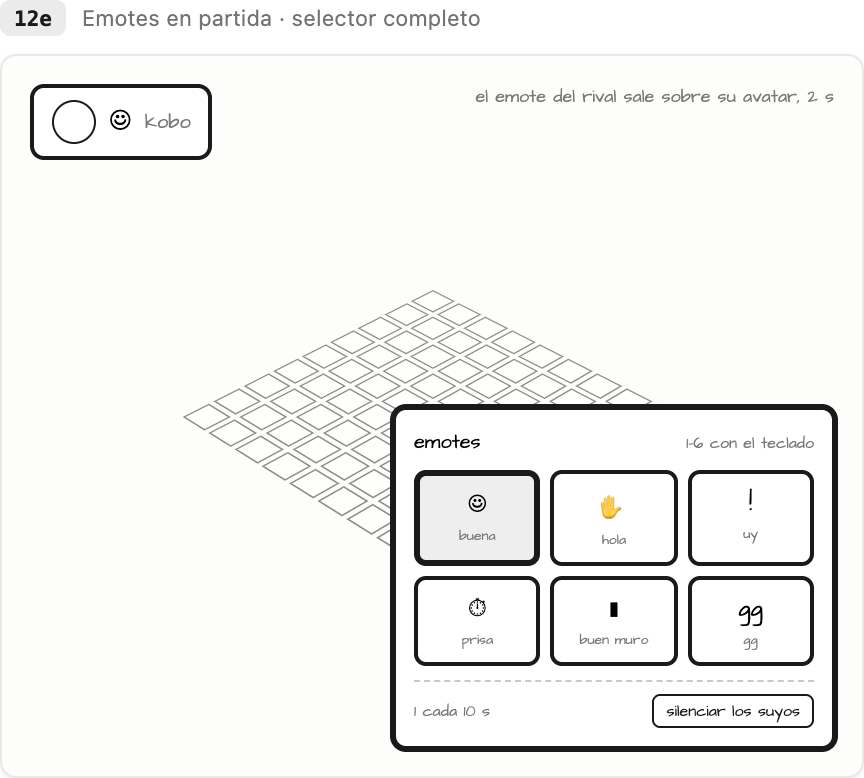
\includegraphics[width=\linewidth]{Prototipos/12e}\par\smallskip
{\footnotesize\RaggedRight \textbf{12e: Emotes en partida}\par Motivo: Enviar un emote no lee ni escribe en la base de datos (\mbox{D-10}).\par}
\end{minipage}\hfill
\begin{minipage}[t]{0.48\textwidth}
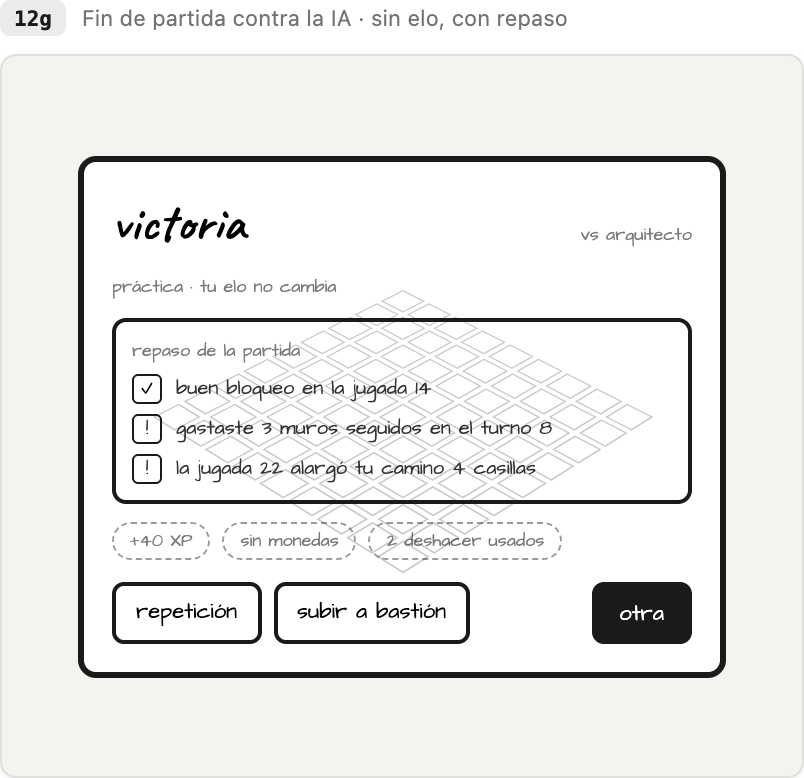
\includegraphics[width=\linewidth]{Prototipos/12g}\par\smallskip
{\footnotesize\RaggedRight \textbf{12g: Fin de partida contra la IA}\par Motivo: Resultado de la partida contra la IA; el repaso se calcula al terminar y no se almacena.\par Sustituida por: 12f, Contra la IA · deshacer y sugerencia.\par}
\end{minipage}
\par
\par\medskip\noindent
\begin{minipage}[t]{0.48\textwidth}
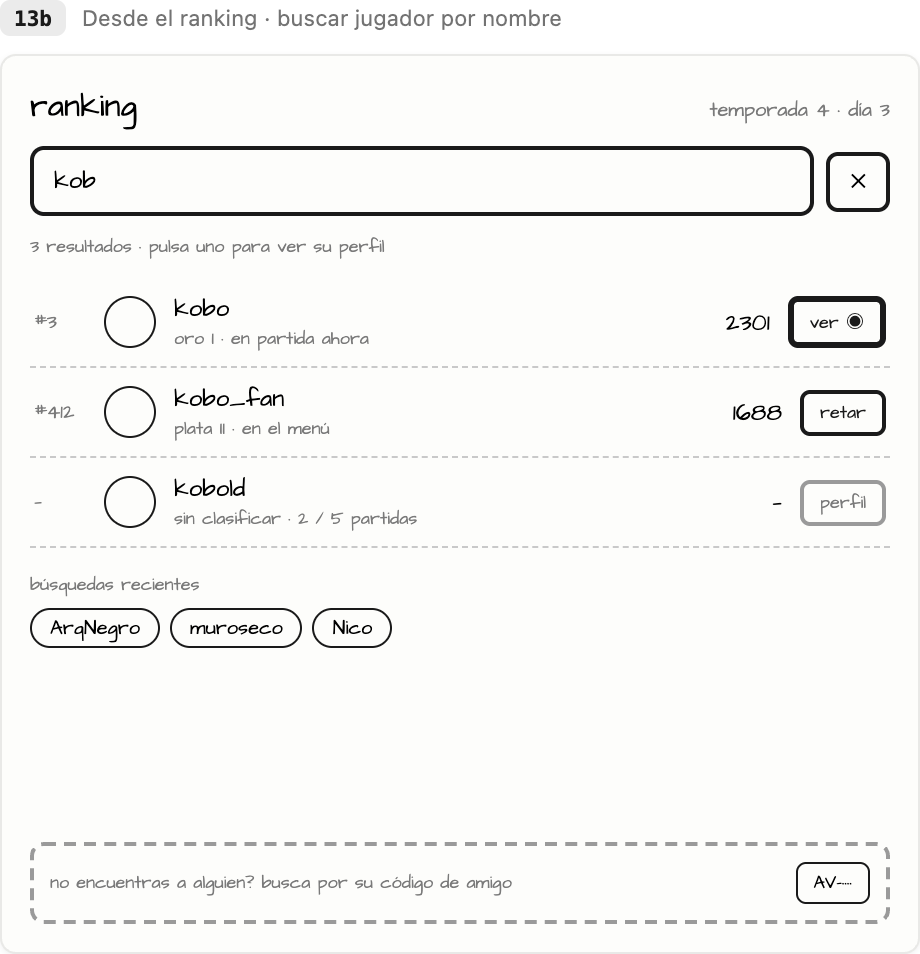
\includegraphics[width=\linewidth]{Prototipos/13b}\par\smallskip
{\footnotesize\RaggedRight \textbf{13b: Desde el ranking · buscar jugador}\par Motivo: Búsqueda sobre la tabla de ranking; mismos datos.\par Sustituida por: 2c, Ranking · tabla con tu fila fijada.\par}
\end{minipage}\hfill
\begin{minipage}[t]{0.48\textwidth}
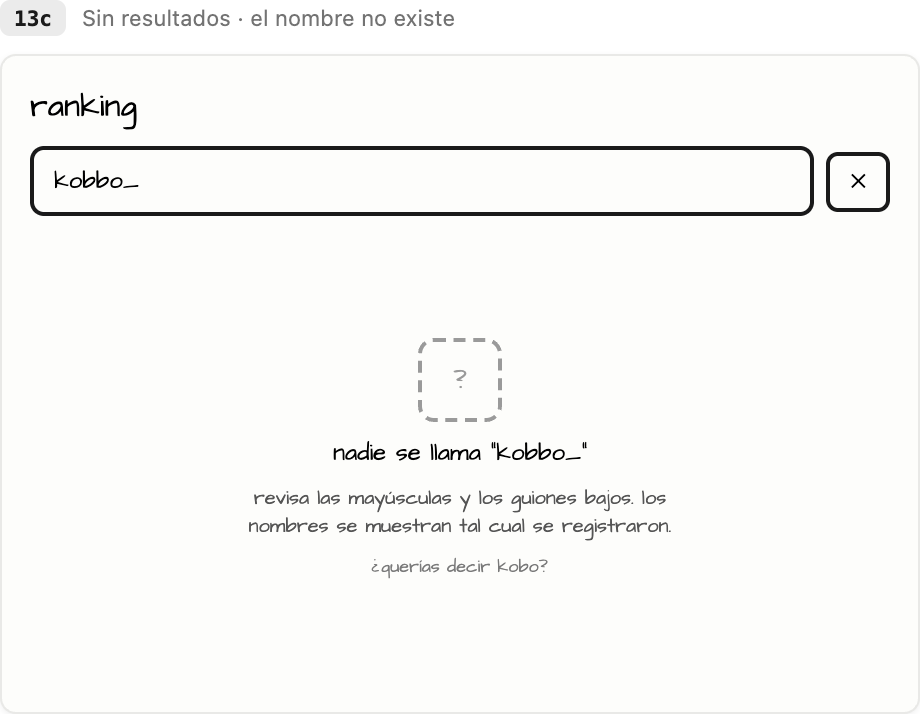
\includegraphics[width=\linewidth]{Prototipos/13c}\par\smallskip
{\footnotesize\RaggedRight \textbf{13c: Búsqueda sin resultados}\par Motivo: Estado vacío de la búsqueda.\par Sustituida por: 2c, Ranking · tabla con tu fila fijada.\par}
\end{minipage}
\par
\par\medskip\noindent
\begin{minipage}[t]{0.48\textwidth}
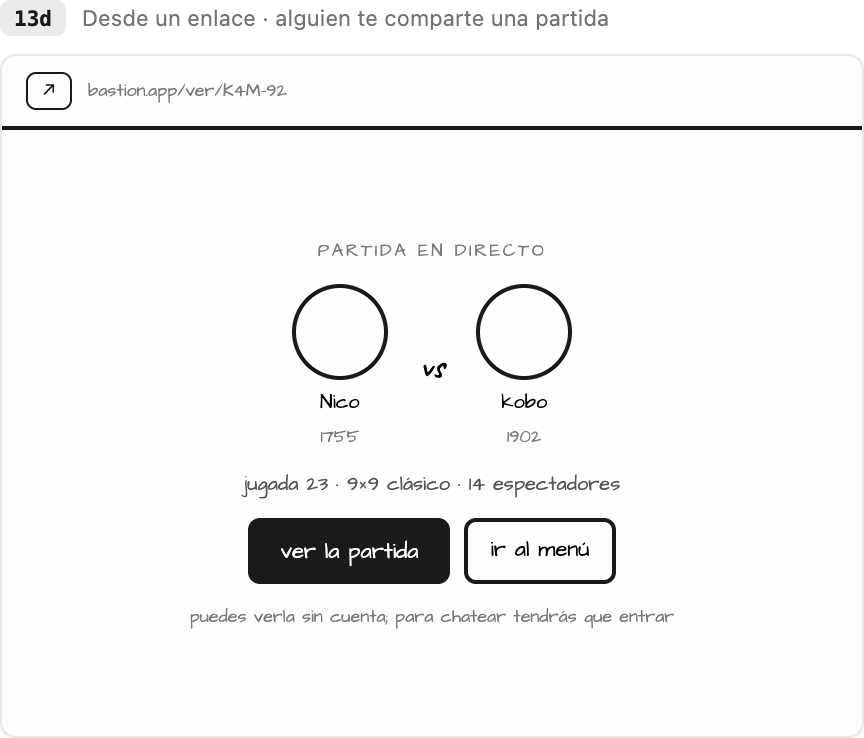
\includegraphics[width=\linewidth]{Prototipos/13d}\par\smallskip
{\footnotesize\RaggedRight \textbf{13d: Desde un enlace compartido}\par Motivo: Entrada por enlace a la misma vista de espectador; el enlace se crea en 13e.\par Sustituida por: 10g, Espectador · con chat de espectadores.\par}
\end{minipage}\hfill
\begin{minipage}[t]{0.48\textwidth}
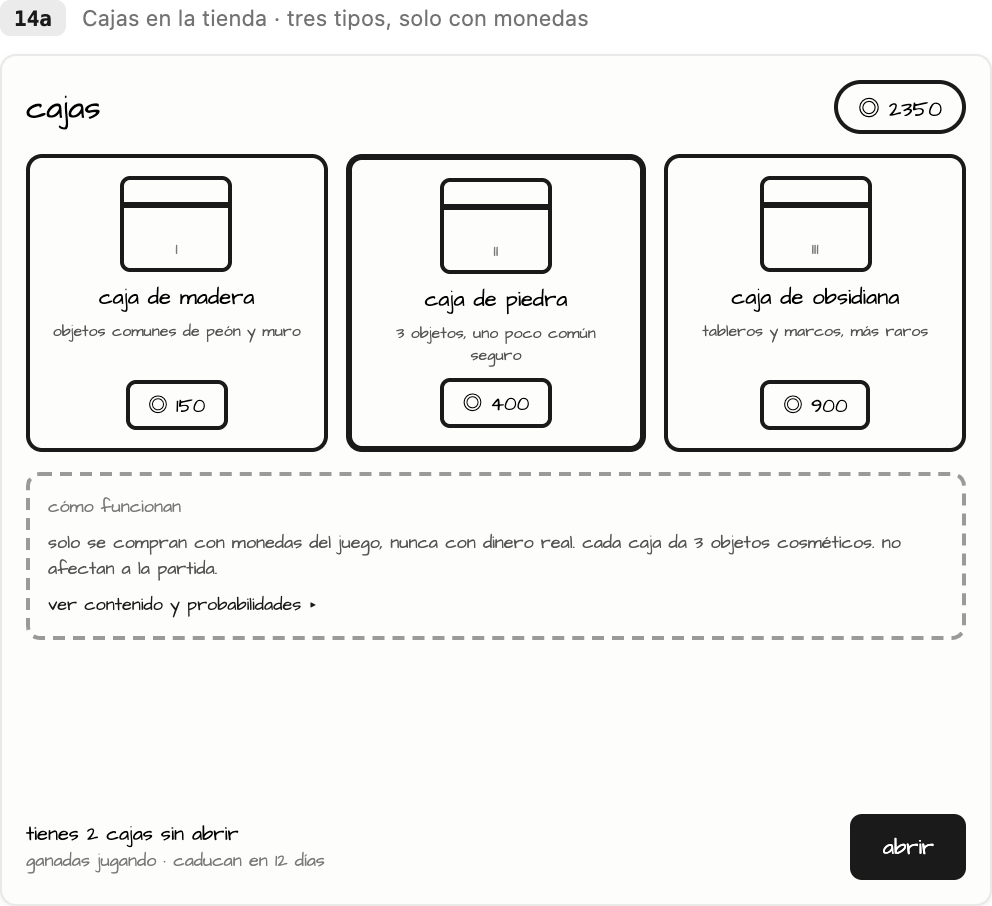
\includegraphics[width=\linewidth]{Prototipos/14a}\par\smallskip
{\footnotesize\RaggedRight \textbf{14a: Cajas en la tienda}\par Motivo: Lista de tipos de caja; sus datos aparecen completos en 14d.\par Sustituida por: 14d, Contenido y probabilidades.\par}
\end{minipage}
\par
\par\medskip\noindent
\begin{minipage}[t]{0.48\textwidth}
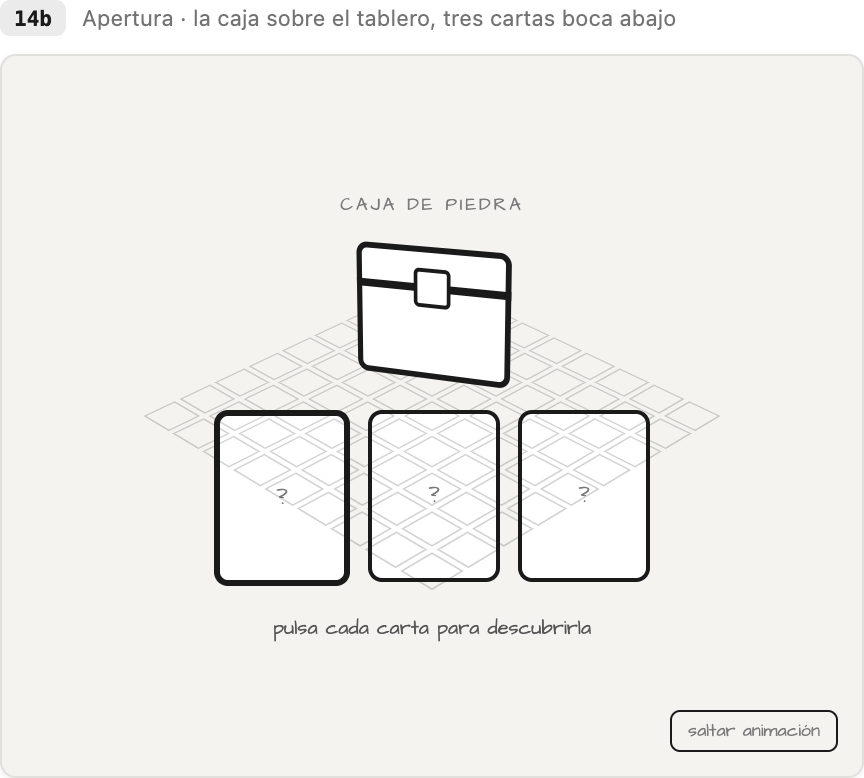
\includegraphics[width=\linewidth]{Prototipos/14b}\par\smallskip
{\footnotesize\RaggedRight \textbf{14b: Apertura de caja}\par Motivo: Animación de apertura; el sorteo ya está hecho en el servidor.\par Sustituida por: 14c, Resultado de la caja.\par}
\end{minipage}\hfill
\begin{minipage}[t]{0.48\textwidth}
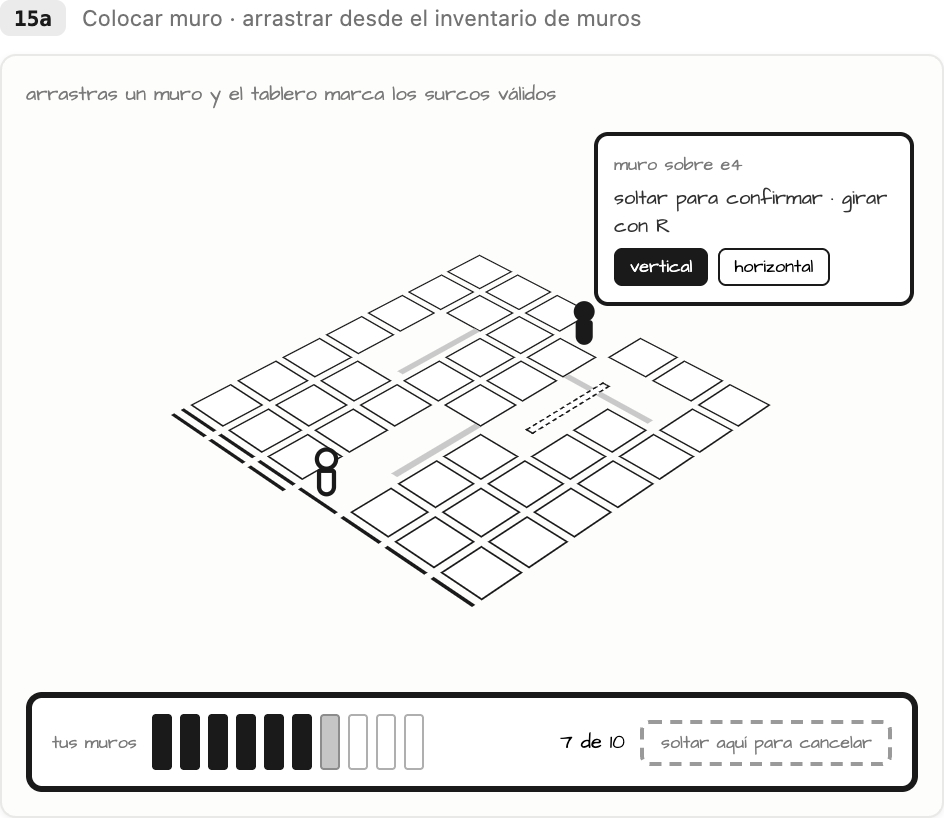
\includegraphics[width=\linewidth]{Prototipos/15a}\par\smallskip
{\footnotesize\RaggedRight \textbf{15a: Colocar muro · arrastrar}\par Motivo: Iteración anterior del gesto de colocar muro, sustituida por el cartel flotante con atajos.\par Sustituida por: 21a, Partida · muro cogido con cartel flotante.\par}
\end{minipage}
\par
\par\medskip\noindent
\begin{minipage}[t]{0.48\textwidth}
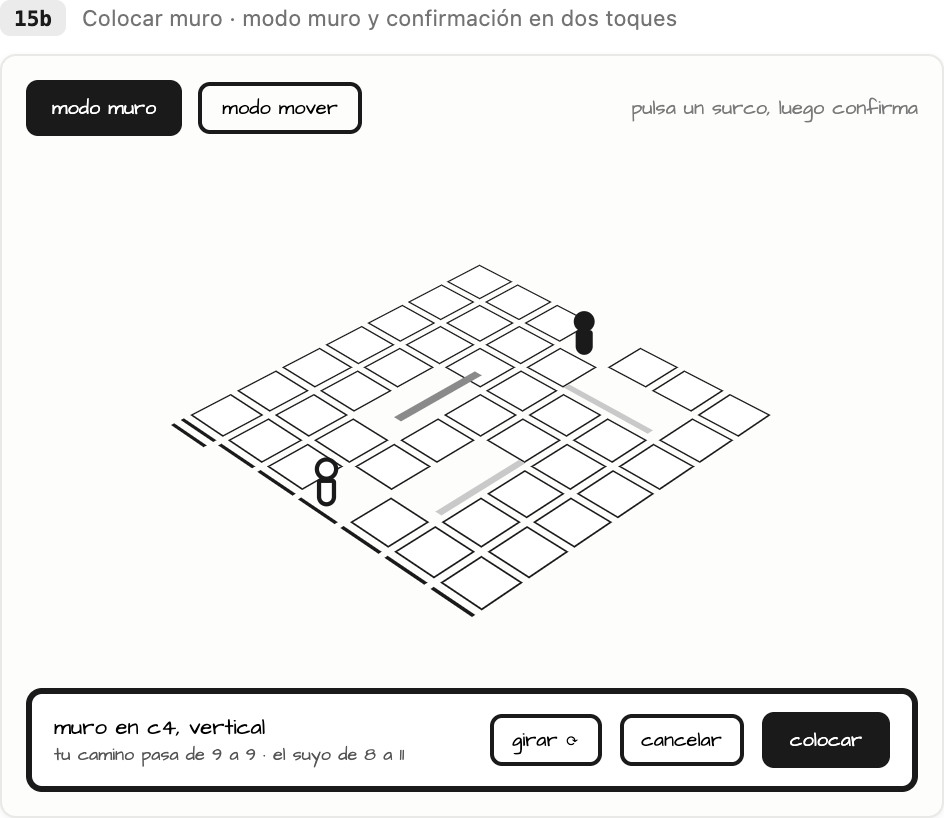
\includegraphics[width=\linewidth]{Prototipos/15b}\par\smallskip
{\footnotesize\RaggedRight \textbf{15b: Colocar muro · modo muro}\par Motivo: Iteración anterior del gesto de colocar muro, sustituida por el cartel flotante con atajos.\par Sustituida por: 21a, Partida · muro cogido con cartel flotante.\par}
\end{minipage}\hfill
\begin{minipage}[t]{0.48\textwidth}
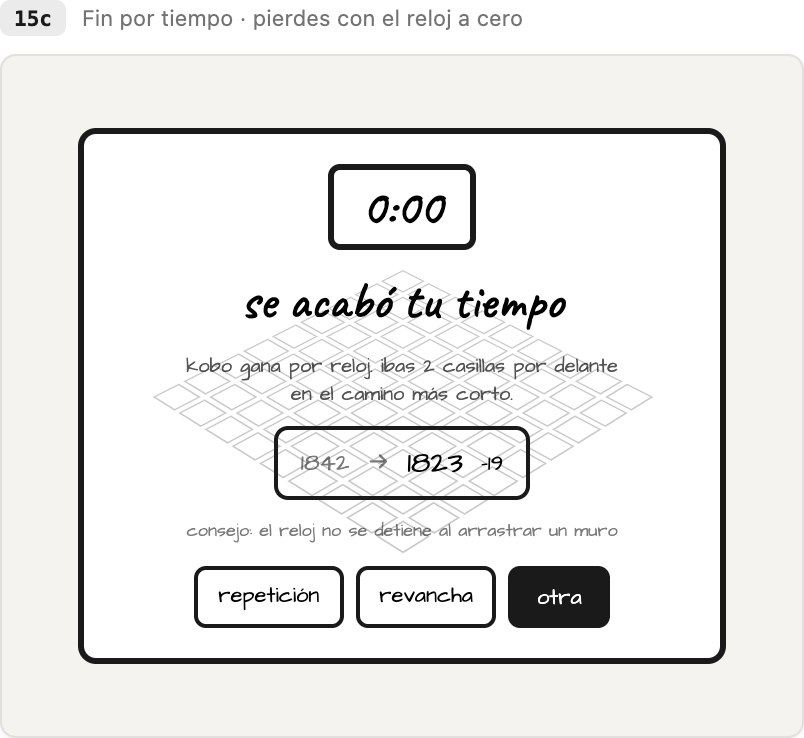
\includegraphics[width=\linewidth]{Prototipos/15c}\par\smallskip
{\footnotesize\RaggedRight \textbf{15c: Fin por tiempo · pierdes}\par Motivo: Variante del fin de partida para una forma de término; solo cambia el valor de forma\_termino.\par Sustituida por: 2g, Fin de partida · tarjeta sobre el tablero.\par}
\end{minipage}
\par
\par\medskip\noindent
\begin{minipage}[t]{0.48\textwidth}
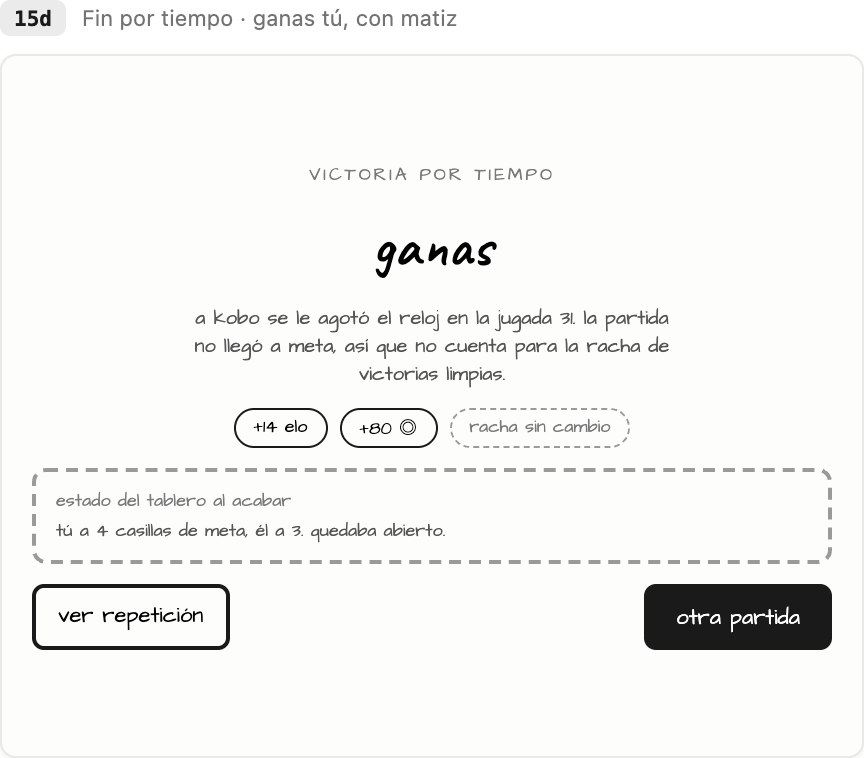
\includegraphics[width=\linewidth]{Prototipos/15d}\par\smallskip
{\footnotesize\RaggedRight \textbf{15d: Fin por tiempo · ganas}\par Motivo: Variante del fin de partida para una forma de término; solo cambia el valor de forma\_termino.\par Sustituida por: 2g, Fin de partida · tarjeta sobre el tablero.\par}
\end{minipage}\hfill
\begin{minipage}[t]{0.48\textwidth}
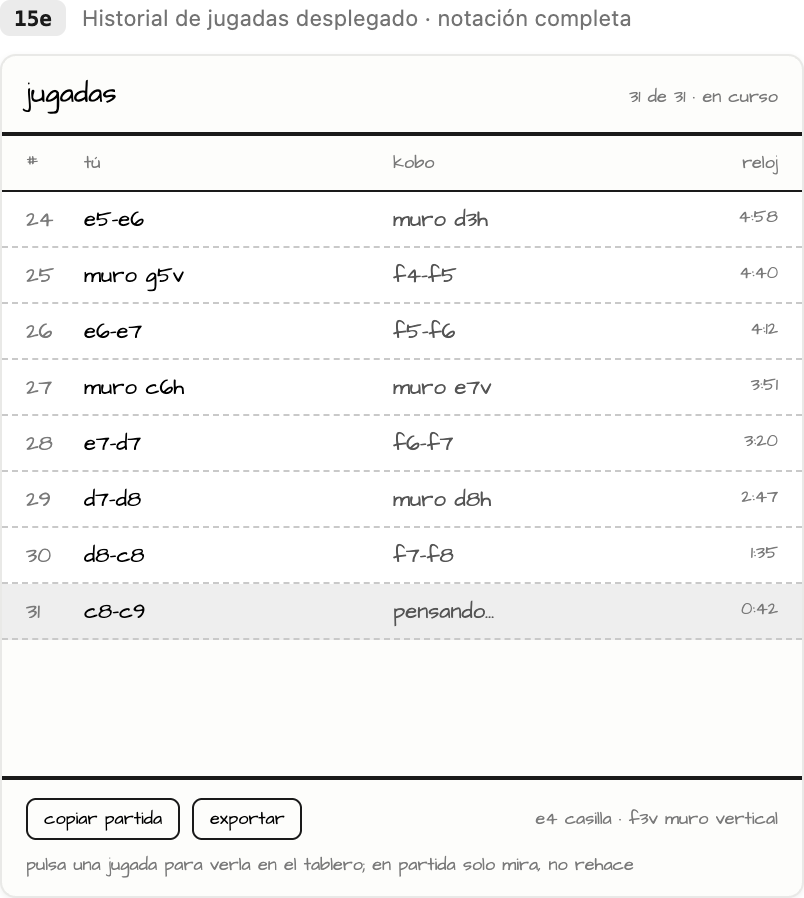
\includegraphics[width=\linewidth]{Prototipos/15e}\par\smallskip
{\footnotesize\RaggedRight \textbf{15e: Historial de jugadas desplegado}\par Motivo: Notación de la partida en curso; lee las mismas jugadas que la repetición.\par Sustituida por: 2f, Repetición · tablero con línea de tiempo.\par}
\end{minipage}
\par
\par\medskip\noindent
\begin{minipage}[t]{0.48\textwidth}
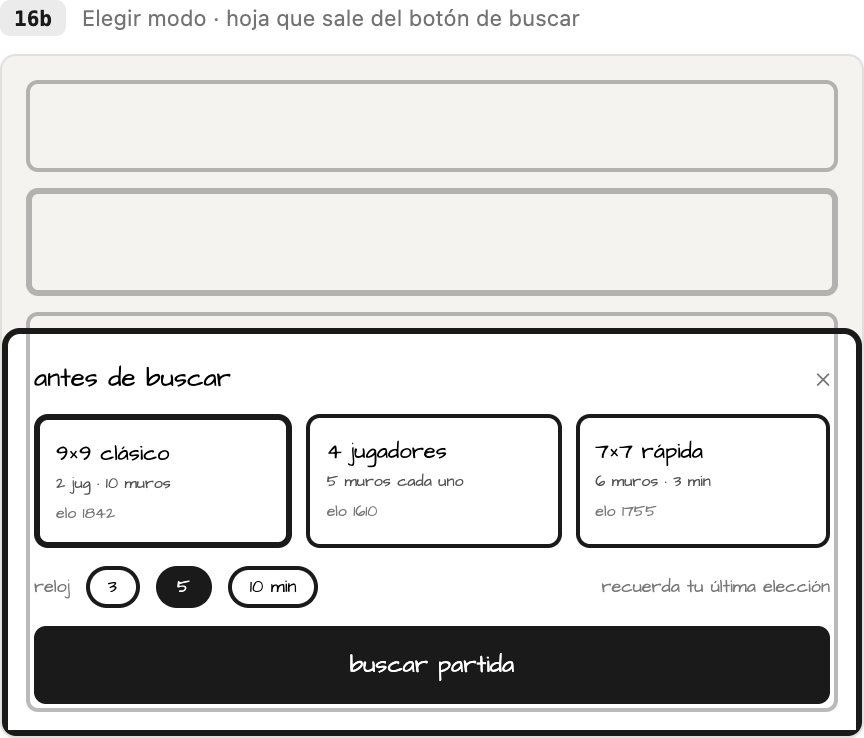
\includegraphics[width=\linewidth]{Prototipos/16b}\par\smallskip
{\footnotesize\RaggedRight \textbf{16b: Elegir modo · hoja rápida}\par Motivo: Variante de disposición de una pantalla ya seleccionada. Muestra los mismos modos y relojes en una hoja compacta.\par Sustituida por: 16a, Elegir modo · pantalla propia.\par}
\end{minipage}\hfill
\begin{minipage}[t]{0.48\textwidth}
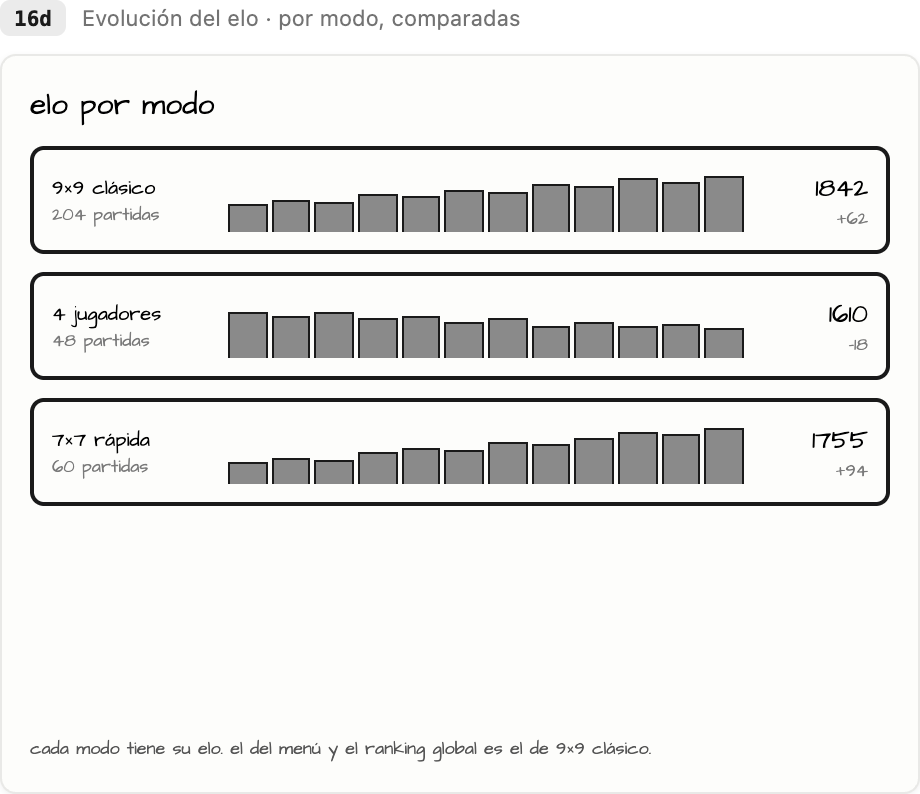
\includegraphics[width=\linewidth]{Prototipos/16d}\par\smallskip
{\footnotesize\RaggedRight \textbf{16d: Evolución del elo por modo}\par Motivo: Amplía la gráfica de 16c comparando modos; lee los mismos datos.\par Sustituida por: 16c, Evolución del elo.\par}
\end{minipage}
\par
\par\medskip\noindent
\begin{minipage}[t]{0.48\textwidth}
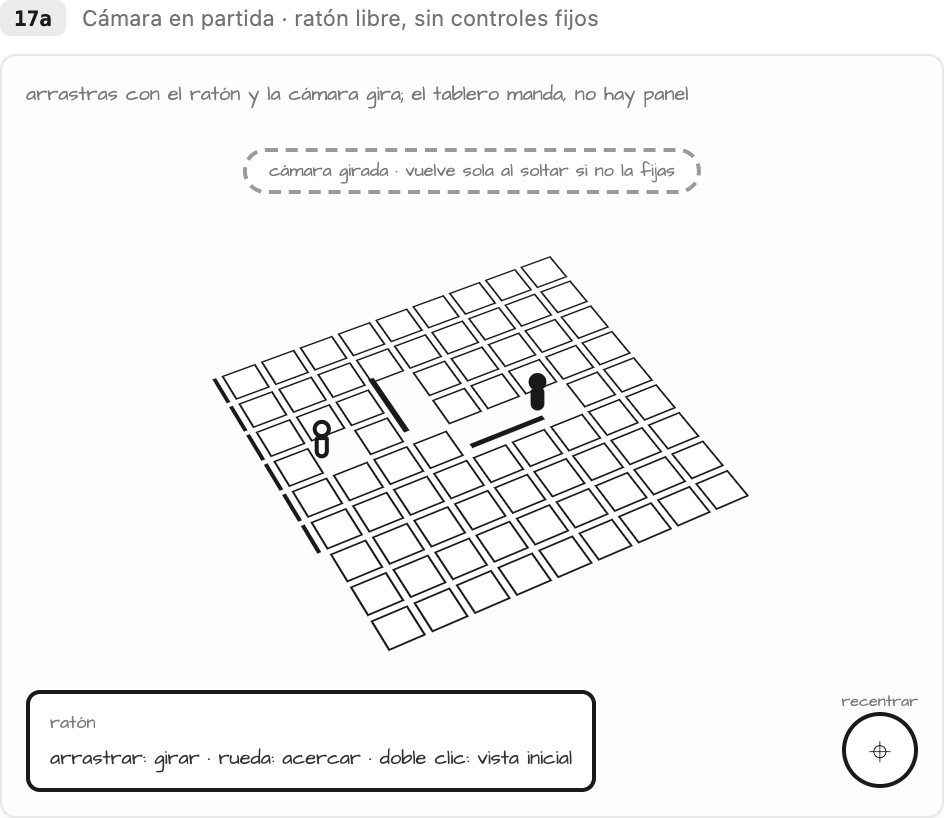
\includegraphics[width=\linewidth]{Prototipos/17a}\par\smallskip
{\footnotesize\RaggedRight \textbf{17a: Cámara en partida}\par Motivo: Configuración local del cliente: no llega a la base de datos.\par}
\end{minipage}\hfill
\begin{minipage}[t]{0.48\textwidth}
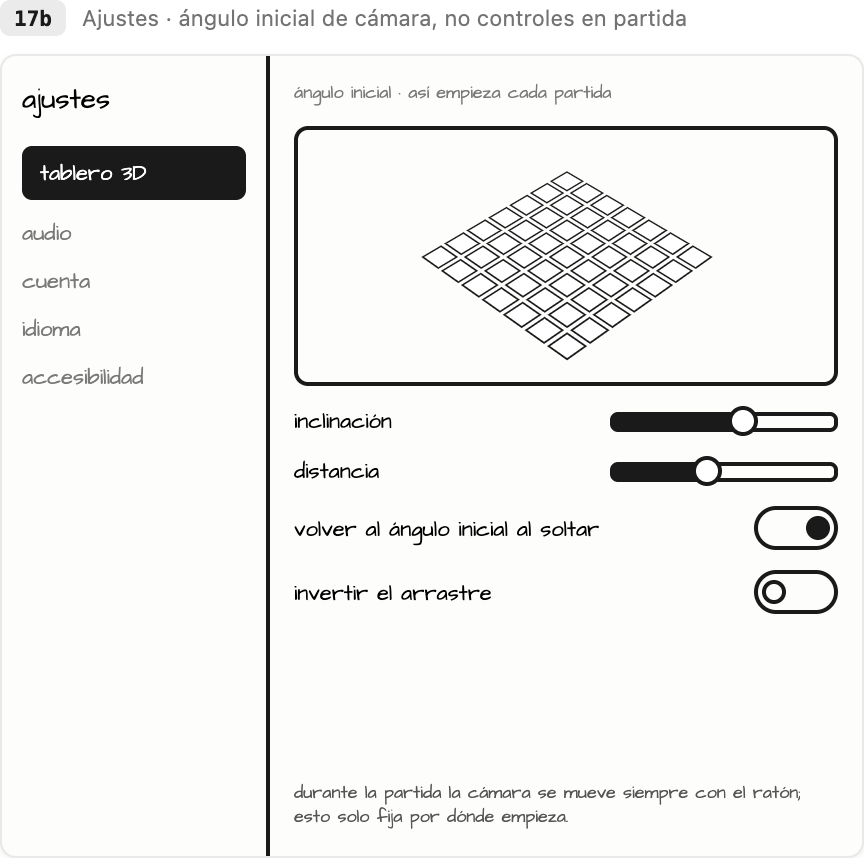
\includegraphics[width=\linewidth]{Prototipos/17b}\par\smallskip
{\footnotesize\RaggedRight \textbf{17b: Ajustes · ángulo de cámara}\par Motivo: Configuración local del cliente: no llega a la base de datos.\par}
\end{minipage}
\par
\par\medskip\noindent
\begin{minipage}[t]{0.48\textwidth}
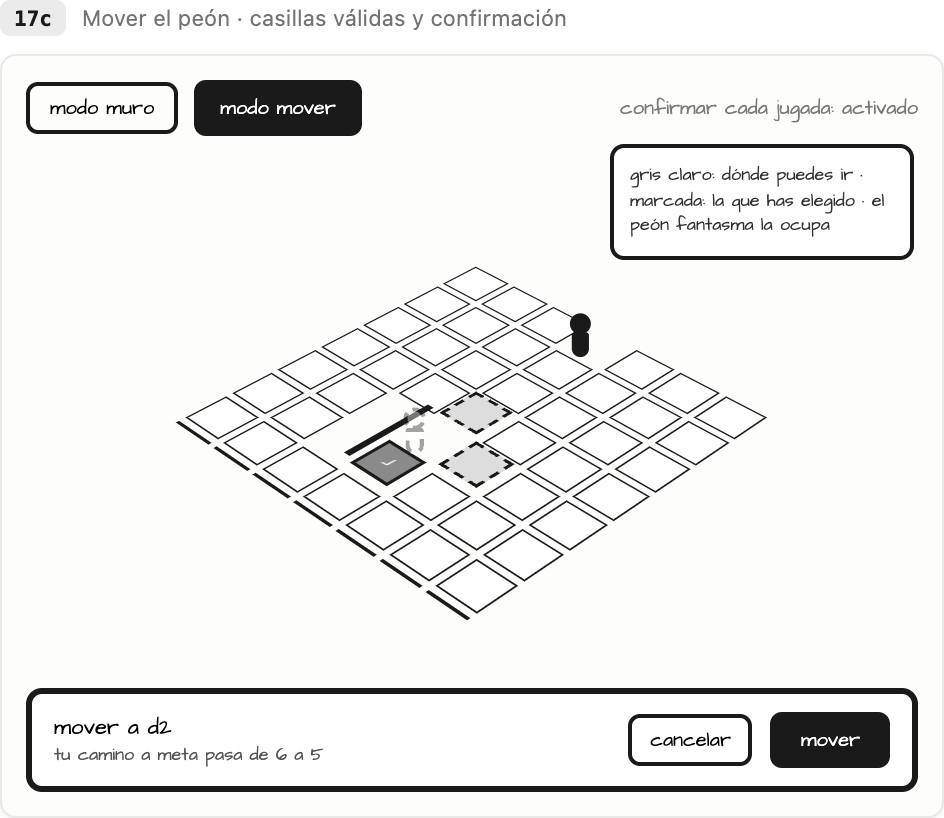
\includegraphics[width=\linewidth]{Prototipos/17c}\par\smallskip
{\footnotesize\RaggedRight \textbf{17c: Mover el peón · modo mover}\par Motivo: Iteración anterior del movimiento del peón, con modos explícitos que el HUD final eliminó.\par Sustituida por: 20a, Partida · peón seleccionado.\par}
\end{minipage}\hfill
\begin{minipage}[t]{0.48\textwidth}
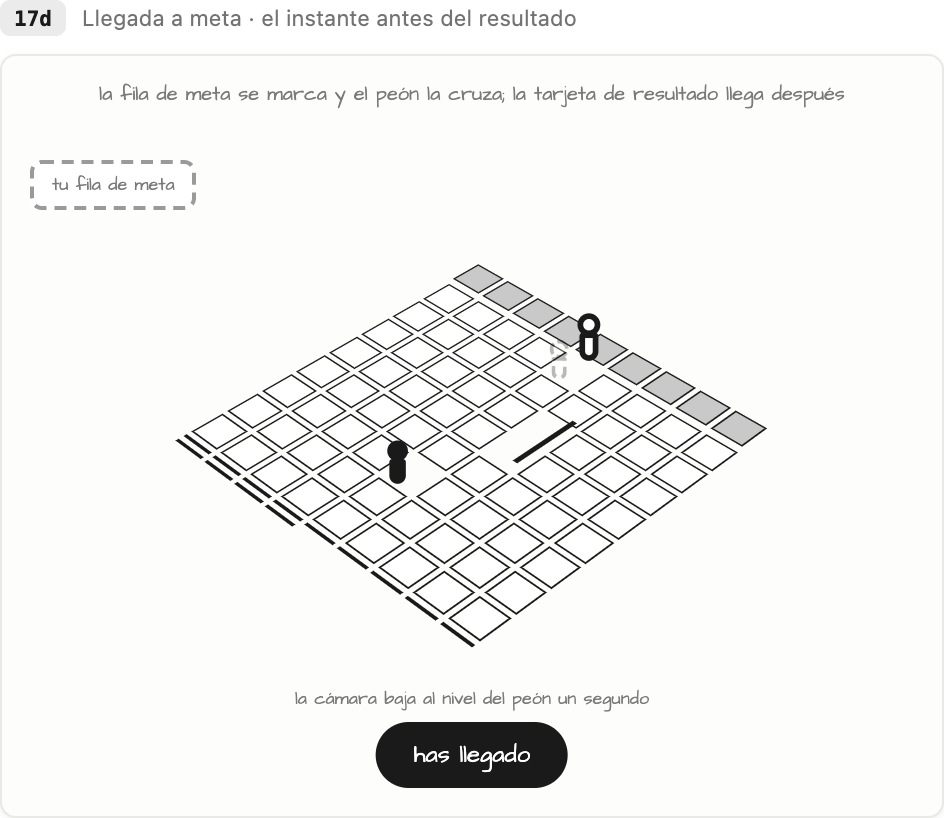
\includegraphics[width=\linewidth]{Prototipos/17d}\par\smallskip
{\footnotesize\RaggedRight \textbf{17d: Llegada a meta}\par Motivo: Estado visual de la partida sin operación de datos propia. Es el instante previo al resultado.\par Sustituida por: 2g, Fin de partida · tarjeta sobre el tablero.\par}
\end{minipage}
\par
\par\medskip\noindent
\begin{minipage}[t]{0.48\textwidth}
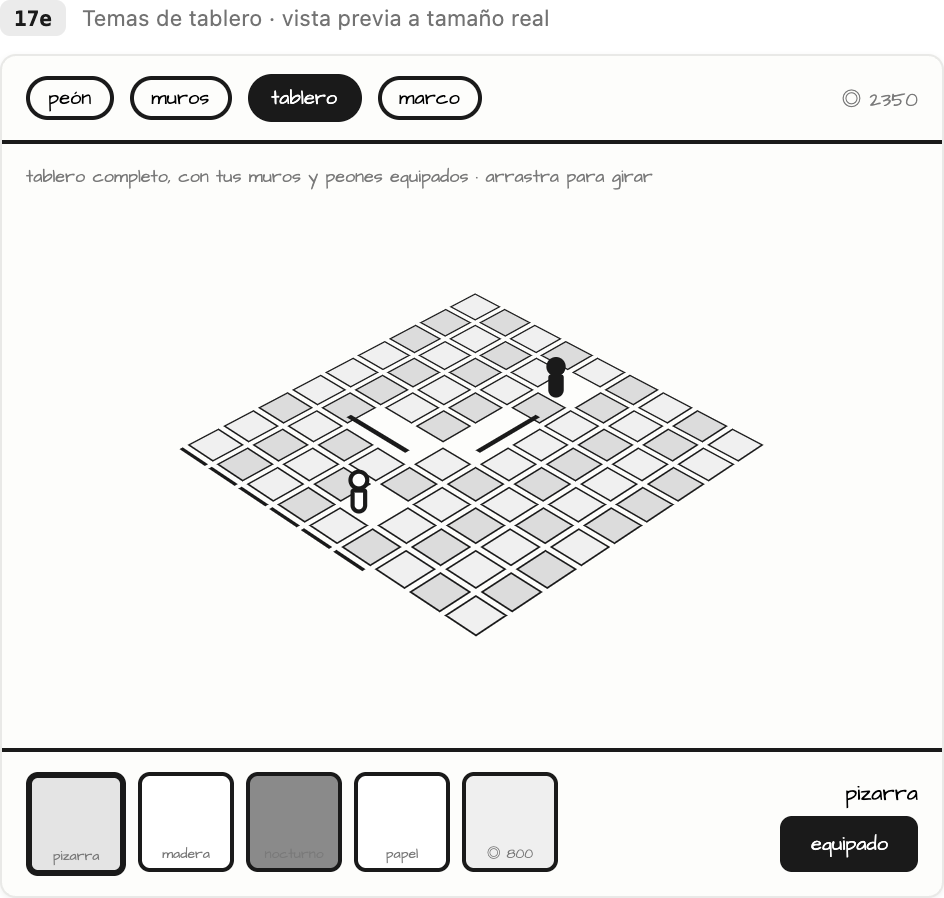
\includegraphics[width=\linewidth]{Prototipos/17e}\par\smallskip
{\footnotesize\RaggedRight \textbf{17e: Temas de tablero · vista previa}\par Motivo: Caso particular de 4a para la ranura de tablero; mismo flujo y mismos datos.\par Sustituida por: 4a, Personalizar · vista previa 3D y rejilla.\par}
\end{minipage}\hfill
\begin{minipage}[t]{0.48\textwidth}
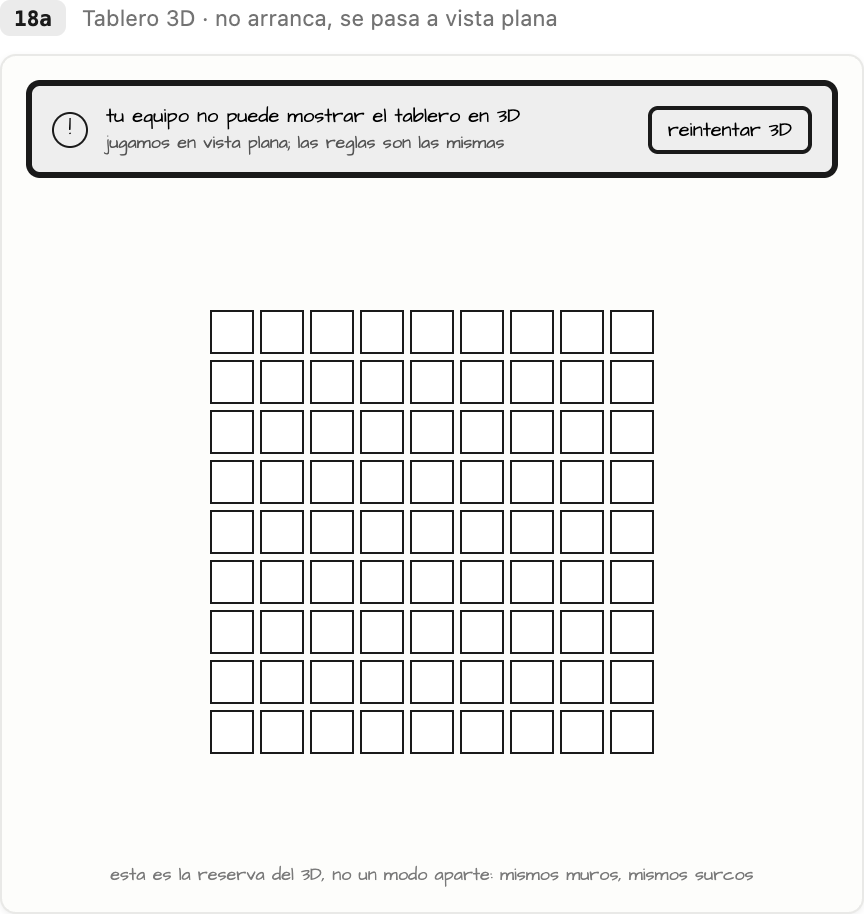
\includegraphics[width=\linewidth]{Prototipos/18a}\par\smallskip
{\footnotesize\RaggedRight \textbf{18a: Errores · tablero 3D no arranca}\par Motivo: Catálogo de mensajes de error y aviso. Documenta los flujos alternos y las excepciones de los casos de uso, no una operación sobre datos.\par}
\end{minipage}
\par
\par\medskip\noindent
\begin{minipage}[t]{0.48\textwidth}
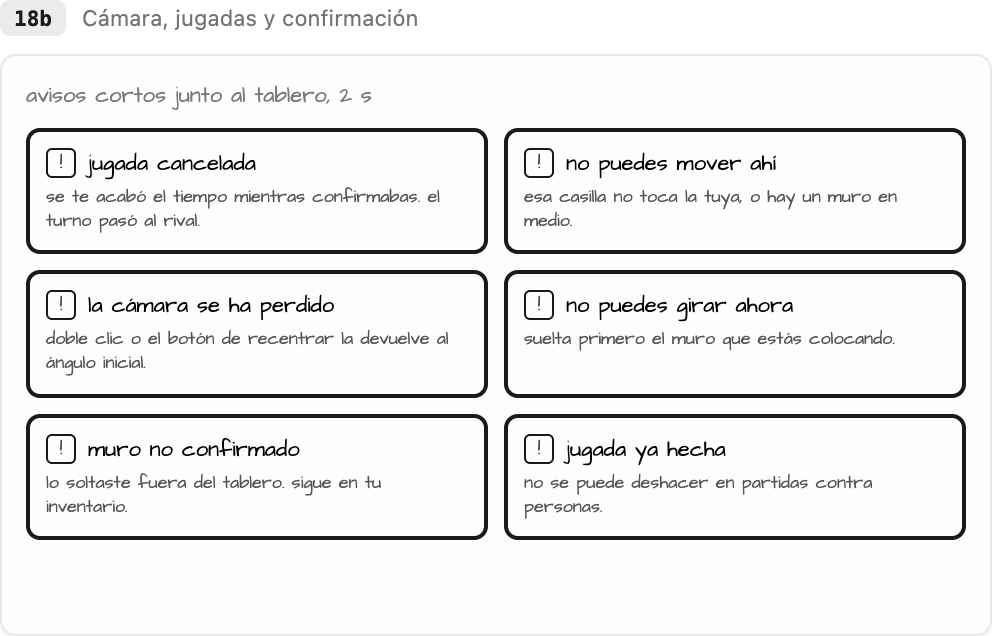
\includegraphics[width=\linewidth]{Prototipos/18b}\par\smallskip
{\footnotesize\RaggedRight \textbf{18b: Errores · cámara, jugadas y confirmación}\par Motivo: Catálogo de mensajes de error y aviso. Documenta los flujos alternos y las excepciones de los casos de uso, no una operación sobre datos.\par}
\end{minipage}\hfill
\begin{minipage}[t]{0.48\textwidth}
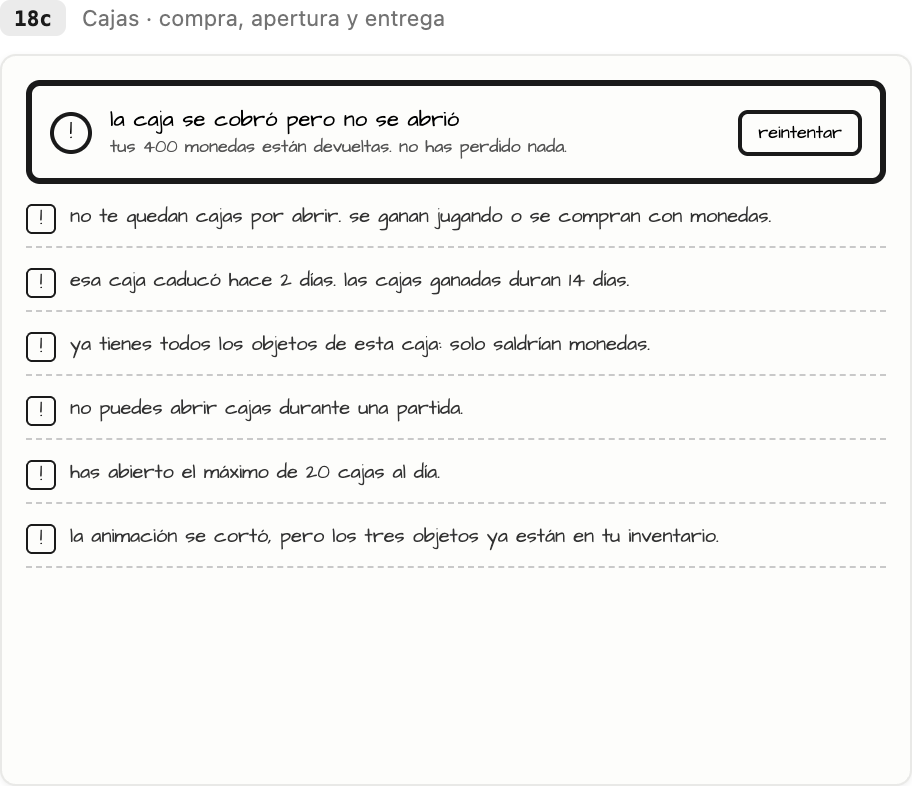
\includegraphics[width=\linewidth]{Prototipos/18c}\par\smallskip
{\footnotesize\RaggedRight \textbf{18c: Errores · cajas}\par Motivo: Catálogo de mensajes de error y aviso. Documenta los flujos alternos y las excepciones de los casos de uso, no una operación sobre datos.\par}
\end{minipage}
\par
\par\medskip\noindent
\begin{minipage}[t]{0.48\textwidth}
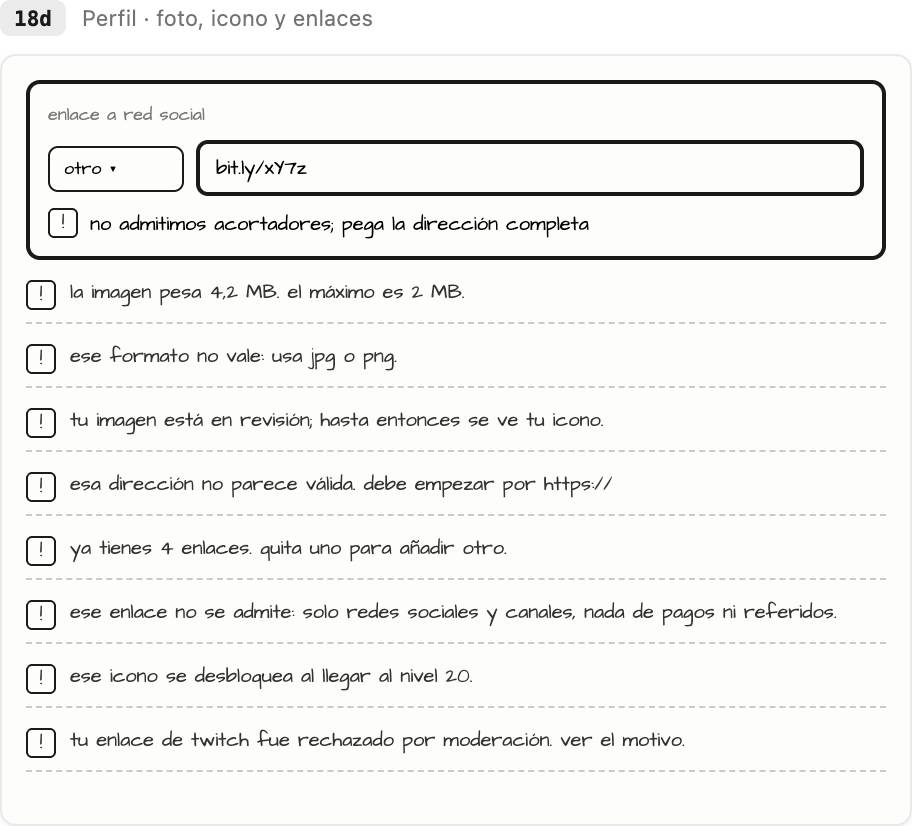
\includegraphics[width=\linewidth]{Prototipos/18d}\par\smallskip
{\footnotesize\RaggedRight \textbf{18d: Errores · perfil}\par Motivo: Catálogo de mensajes de error y aviso. Documenta los flujos alternos y las excepciones de los casos de uso, no una operación sobre datos.\par}
\end{minipage}\hfill
\begin{minipage}[t]{0.48\textwidth}
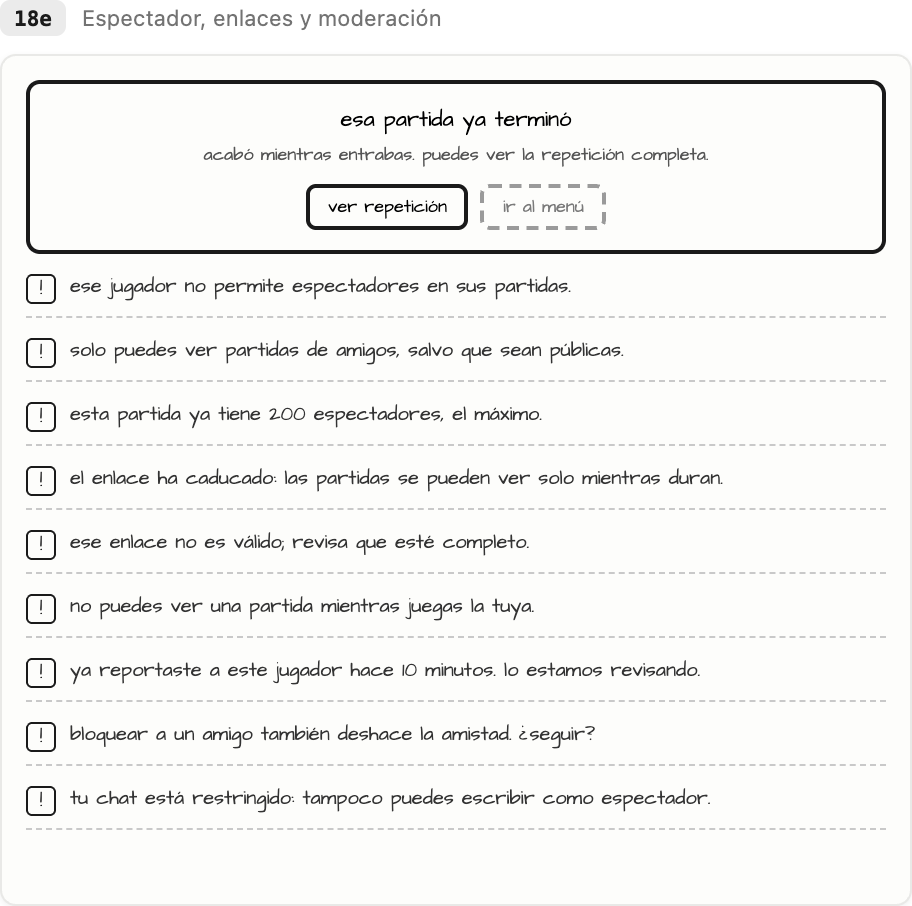
\includegraphics[width=\linewidth]{Prototipos/18e}\par\smallskip
{\footnotesize\RaggedRight \textbf{18e: Errores · espectador, enlaces y moderación}\par Motivo: Catálogo de mensajes de error y aviso. Documenta los flujos alternos y las excepciones de los casos de uso, no una operación sobre datos.\par}
\end{minipage}
\par
\par\medskip\noindent
\begin{minipage}[t]{0.48\textwidth}
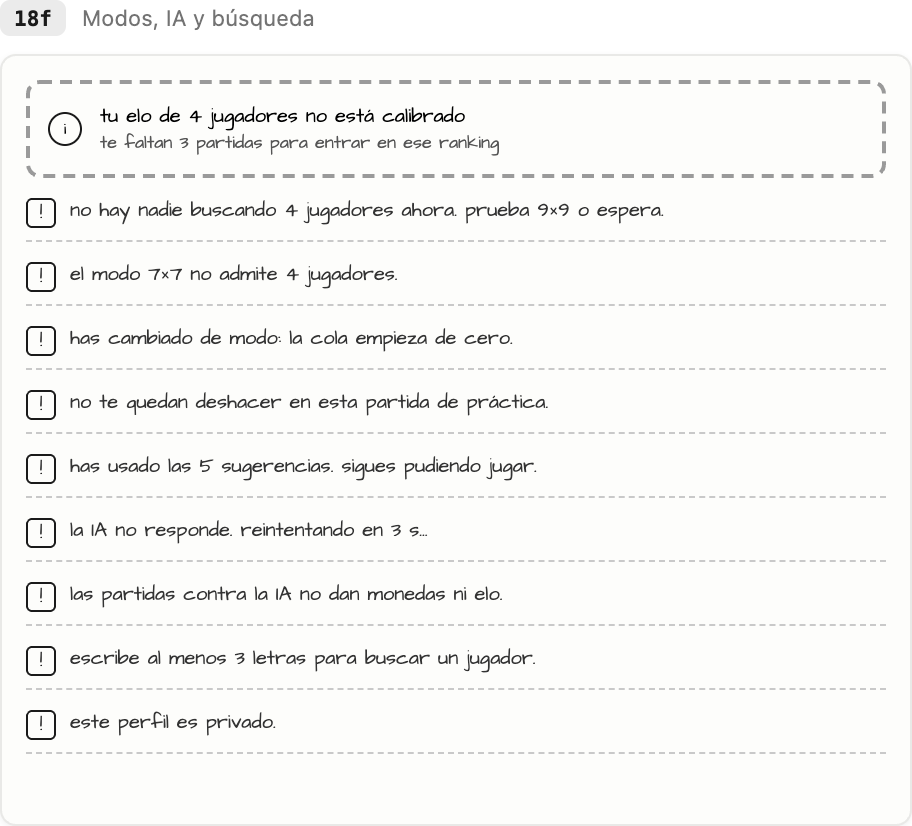
\includegraphics[width=\linewidth]{Prototipos/18f}\par\smallskip
{\footnotesize\RaggedRight \textbf{18f: Errores · modos, IA y búsqueda}\par Motivo: Catálogo de mensajes de error y aviso. Documenta los flujos alternos y las excepciones de los casos de uso, no una operación sobre datos.\par}
\end{minipage}\hfill
\begin{minipage}[t]{0.48\textwidth}
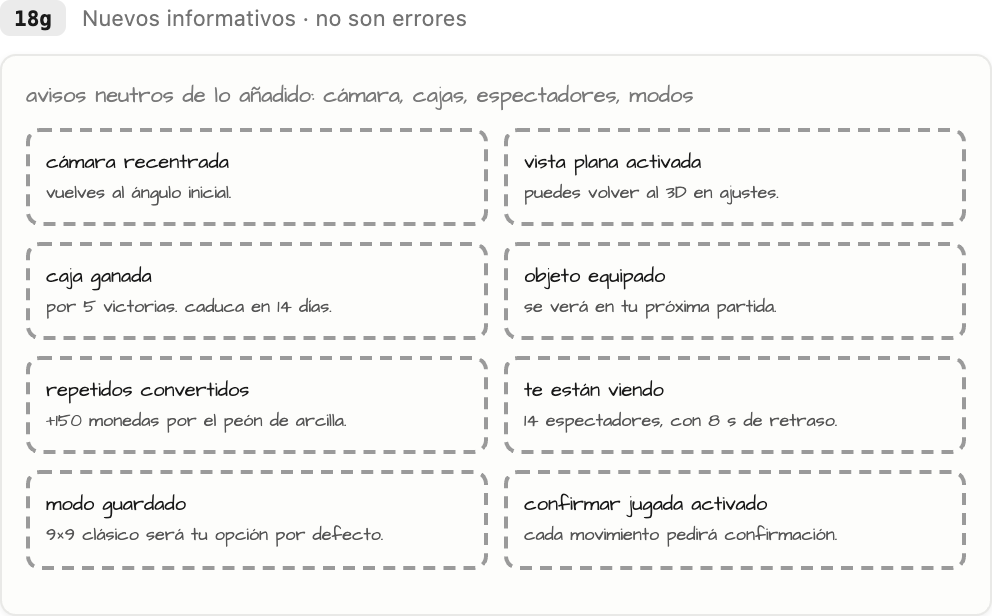
\includegraphics[width=\linewidth]{Prototipos/18g}\par\smallskip
{\footnotesize\RaggedRight \textbf{18g: Nuevos avisos informativos}\par Motivo: Catálogo de mensajes de error y aviso. Documenta los flujos alternos y las excepciones de los casos de uso, no una operación sobre datos.\par}
\end{minipage}
\par
\par\medskip\noindent
\begin{minipage}[t]{0.48\textwidth}
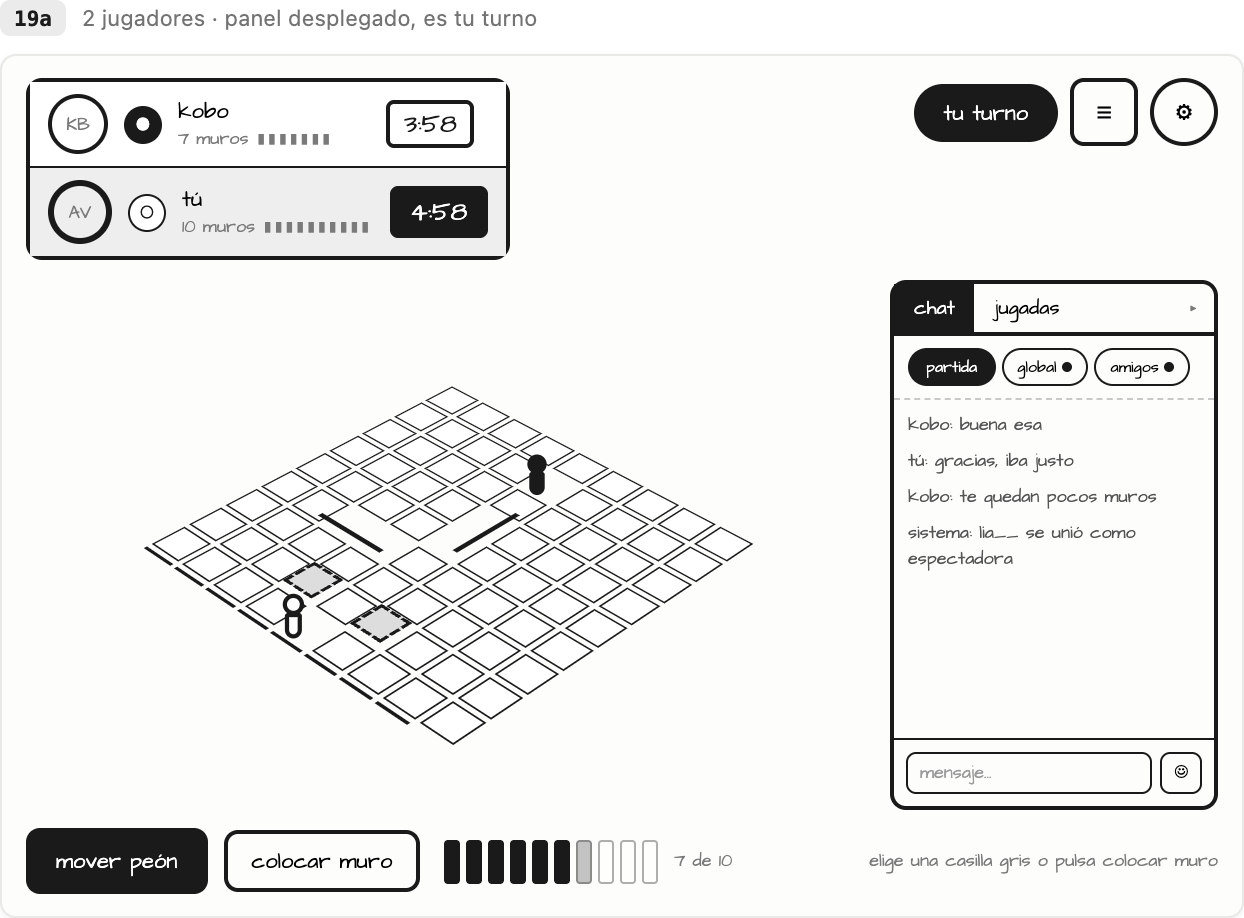
\includegraphics[width=\linewidth]{Prototipos/19a}\par\smallskip
{\footnotesize\RaggedRight \textbf{19a: Partida · panel desplegado}\par Motivo: Iteración anterior del HUD de partida, sustituida por las pantallas 20 y 21, que son las que describe el documento de diseño.\par Sustituida por: 20a, Partida · peón seleccionado.\par}
\end{minipage}\hfill
\begin{minipage}[t]{0.48\textwidth}
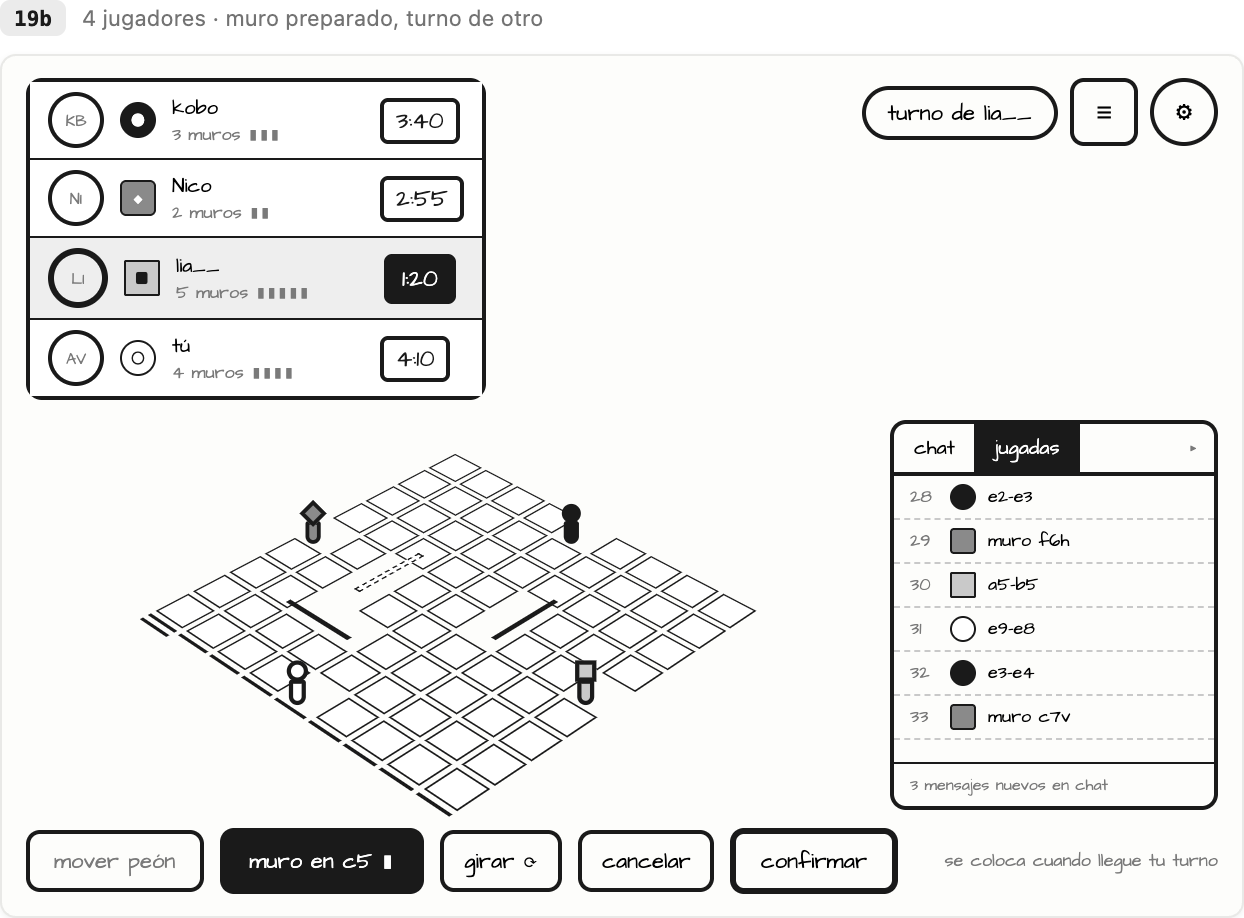
\includegraphics[width=\linewidth]{Prototipos/19b}\par\smallskip
{\footnotesize\RaggedRight \textbf{19b: Partida · 4 jugadores, muro preparado}\par Motivo: Iteración anterior del HUD de partida, sustituida por las pantallas 20 y 21, que son las que describe el documento de diseño.\par Sustituida por: 21a, Partida · muro cogido con cartel flotante.\par}
\end{minipage}
\par
\par\medskip\noindent
\begin{minipage}[t]{0.48\textwidth}
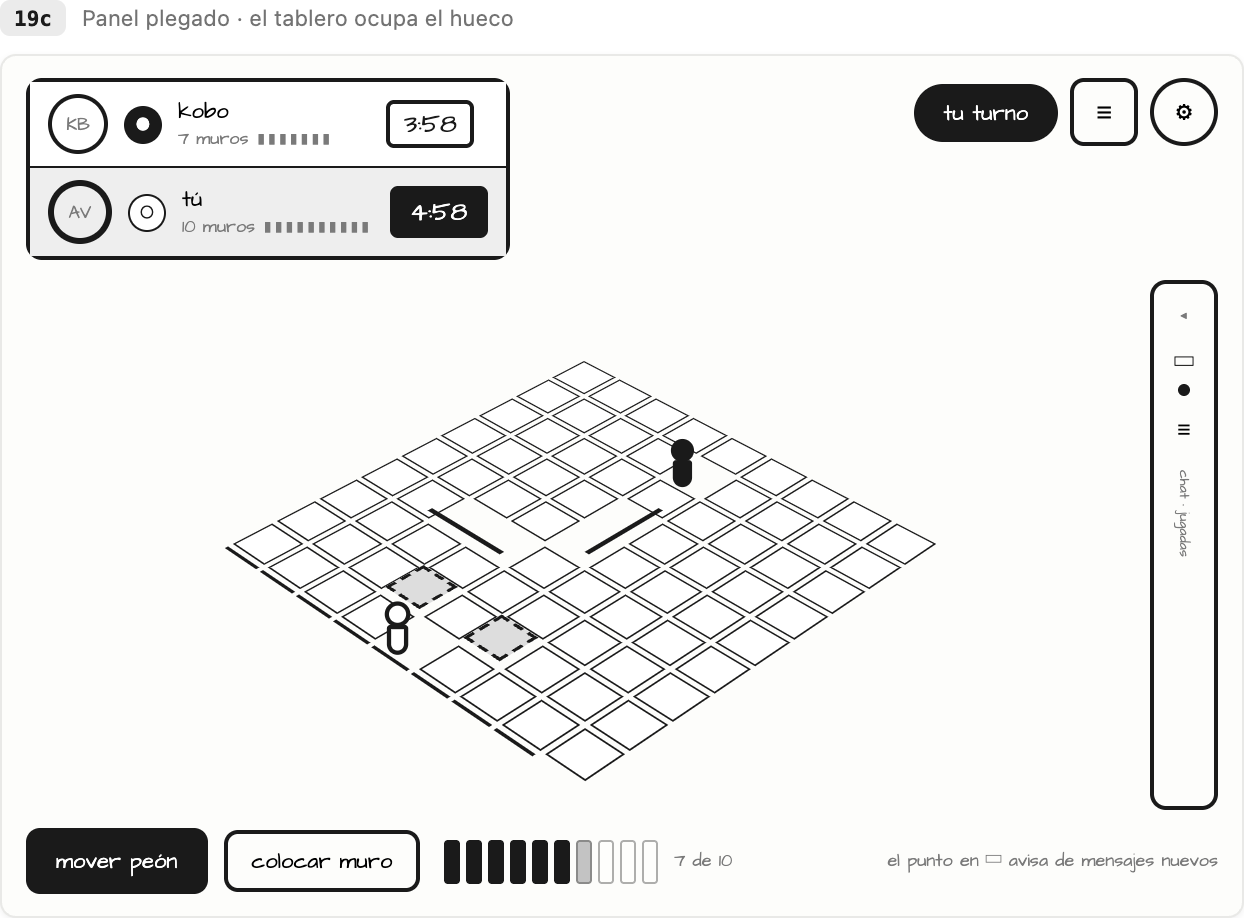
\includegraphics[width=\linewidth]{Prototipos/19c}\par\smallskip
{\footnotesize\RaggedRight \textbf{19c: Partida · panel plegado}\par Motivo: Iteración anterior del HUD de partida, sustituida por las pantallas 20 y 21, que son las que describe el documento de diseño.\par Sustituida por: 20a, Partida · peón seleccionado.\par}
\end{minipage}\hfill
\begin{minipage}[t]{0.48\textwidth}
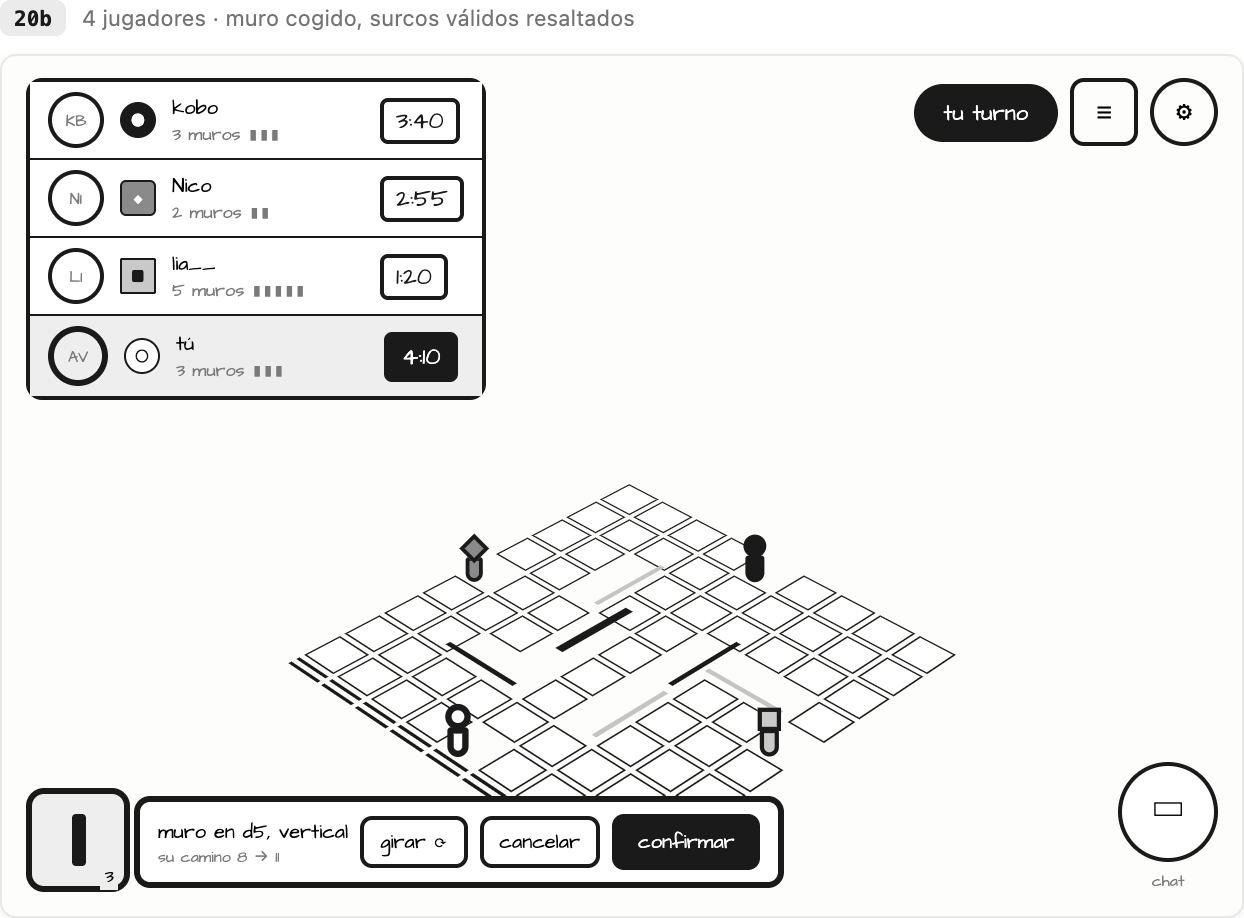
\includegraphics[width=\linewidth]{Prototipos/20b}\par\smallskip
{\footnotesize\RaggedRight \textbf{20b: Partida · 4 jugadores, muro cogido}\par Motivo: Mismo gesto que 21a en una partida de cuatro jugadores; registra la misma Jugada.\par Sustituida por: 21a, Partida · muro cogido con cartel flotante.\par}
\end{minipage}
\par
\par\medskip\noindent
\begin{minipage}[t]{0.48\textwidth}
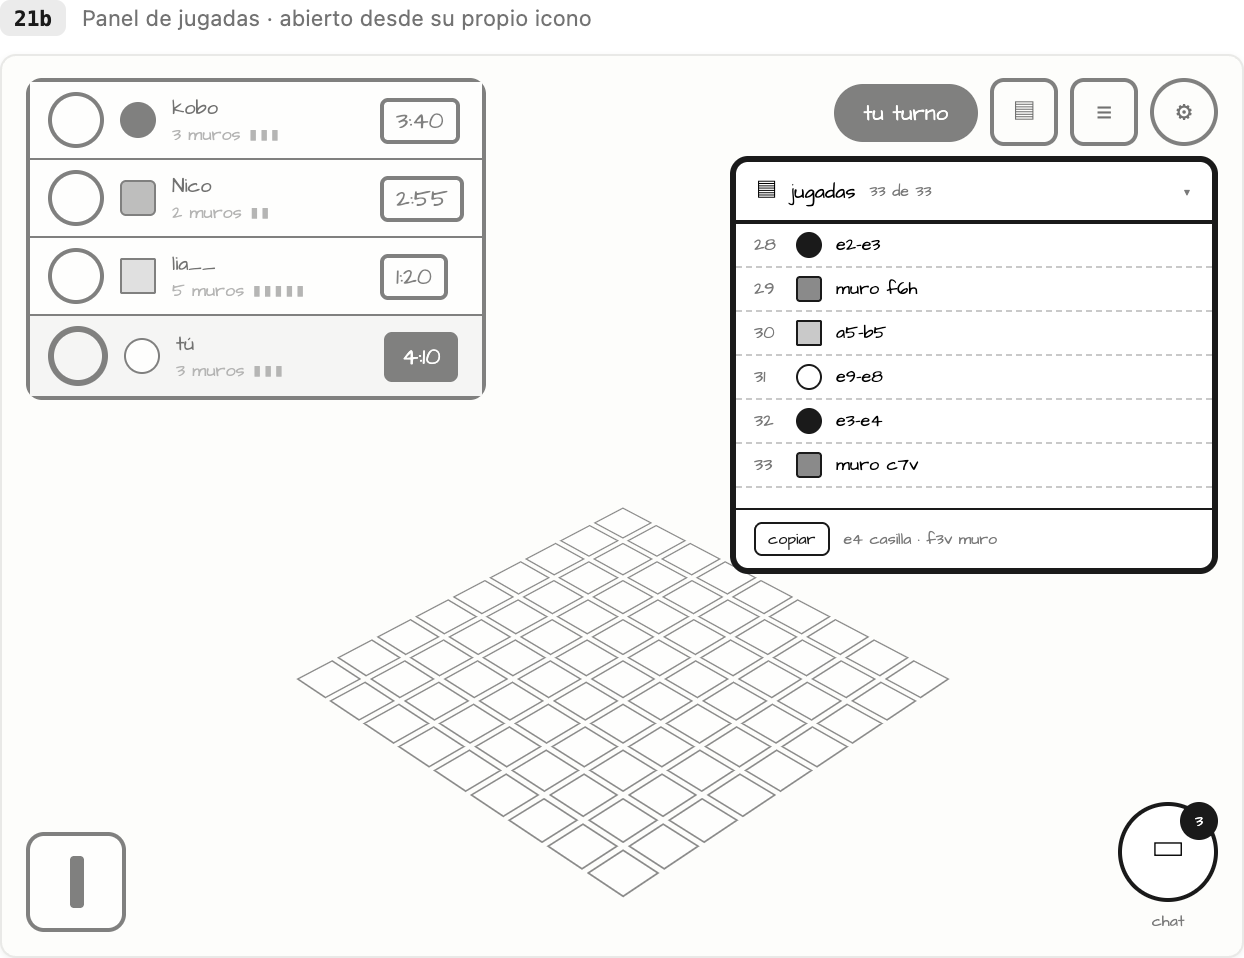
\includegraphics[width=\linewidth]{Prototipos/21b}\par\smallskip
{\footnotesize\RaggedRight \textbf{21b: Panel de jugadas desde su icono}\par Motivo: Panel de jugadas dentro de la partida; lee las mismas jugadas que la repetición.\par Sustituida por: 2f, Repetición · tablero con línea de tiempo.\par}
\end{minipage}\hfill
\begin{minipage}[t]{0.48\textwidth}
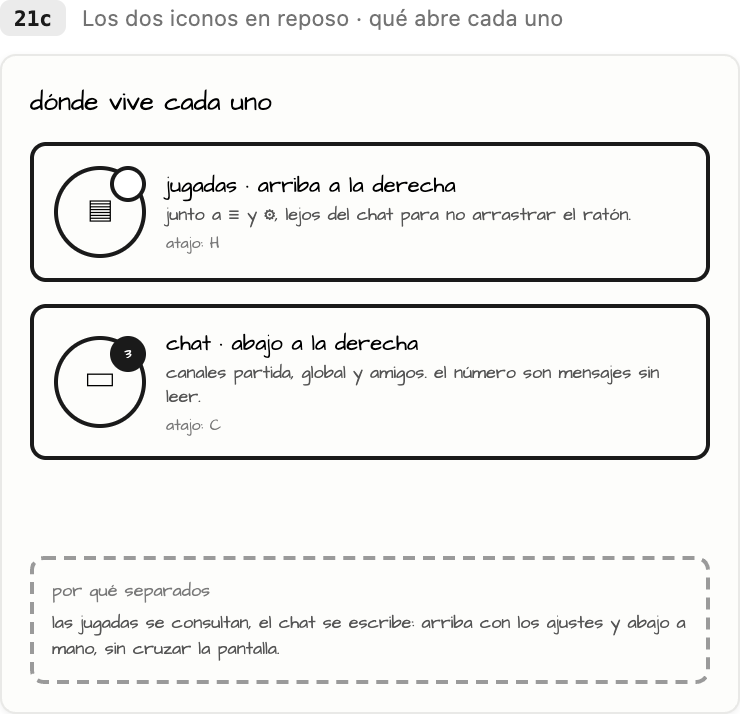
\includegraphics[width=\linewidth]{Prototipos/21c}\par\smallskip
{\footnotesize\RaggedRight \textbf{21c: Los dos iconos en reposo}\par Motivo: Explica la ubicación de los iconos; no muestra datos.\par}
\end{minipage}
\par

\subsubsection*{Diferencias entre prototipos y casos de uso}
\addcontentsline{toc}{subsubsection}{Diferencias entre prototipos y casos de uso}
Al revisar las pantallas se encontraron diferencias con lo especificado en los casos de uso. Mandan los casos de uso; las pantallas deben corregirse en la siguiente versión del prototipo.

\begin{center}\small
\begin{longtable}{|L{0.13\textwidth}|L{0.61\textwidth}|L{0.16\textwidth}|}
\hline
\textbf{Prototipo} & \textbf{Diferencia} & \textbf{Caso} \\ \hline
\endfirsthead
\hline
\textbf{Prototipo} & \textbf{Diferencia} & \textbf{Caso} \\ \hline
\endhead
6c & La pantalla de inicio no tiene campos de identificador ni contraseña, y no hay prototipo del formulario de registro. & \mbox{CU-01}, \mbox{CU-02} \\ \hline
6d & Pide el nombre en la primera vez. Los casos lo piden en el registro y la primera vez solo elige peón e icono (\mbox{D-13}). & \mbox{CU-08} \\ \hline
9e & La vinculación solo pide correo y contraseña. El caso pide además el nickname definitivo y la fecha de nacimiento. & \mbox{CU-07} \\ \hline
9f & Incluye ``descargar mis datos'', retirado del alcance, y dice que borrar la cuenta ``no tiene vuelta atrás'', cuando es recuperable catorce días (\mbox{D-07}). & \mbox{CU-11} \\ \hline
7e & El nombre admite de 3 a 16 caracteres y el bloqueo por intentos es de 60 segundos. Los casos fijan de 3 a 30 caracteres y un bloqueo escalonado de 5, 30 y 60 minutos. & \mbox{CU-01}, \mbox{CU-02} \\ \hline
7d & El código de sala tiene la forma K4M-93. El caso fija seis caracteres alfanuméricos. & \mbox{CU-19} \\ \hline
2c, 16c & Mencionan temporadas. El ranking no tiene temporadas. & \mbox{CU-35} \\ \hline
18f & Limita las sugerencias contra la IA a cinco y menciona perfiles privados; ninguna de las dos cosas está en los casos. & \mbox{CU-27}, \mbox{CU-16} \\ \hline
19d & Solo permite ofrecer tablas desde la jugada 10. El caso permite ofrecerlas en cualquier momento, una vez cada cinco jugadas propias. & \mbox{CU-22} \\ \hline
10a & El menú de un jugador no incluye ``eliminar amigo''. & \mbox{CU-49} \\ \hline
\end{longtable}
\end{center}

